\chapter{ผลการดำเนินงานของหลักสูตร}

\begin{center}
(เกณฑ์มาตรฐานหลักสูตรระดับอุดมศึกษา พ.ศ. 2558)\\[1cm]
การรายงานผลการดำเนินงานของ\\ \printprogram{} \\
\printfaculty{}  \printuniversity{}\\
ประจำปีการศึกษา \printyear{} วันที่รายงาน \printrepdate{}
\end{center}

\section{ข้อมูลทั่วไป}

\subsection*{รหัสหลักสูตร}
25511911104688

\subsection*{อาจารย์ผู้รับผิดชอบหลักสูตร}


\begin{longtable}{|l|l|p{0.3\textwidth}|}
\hline
\multicolumn{1}{|c|}{\textbf{มคอ. 2}}                  & \multicolumn{1}{c|}{\textbf{ปัจจุบัน}}                    &\begin{tabular}[c]{@{}c@{}}\textbf{หมายเหตุ}\\ (วันที่เปลี่ยนแปลงพร้อมเหตุผล)\end{tabular}                                        \\ \hline


1. นายสมนึก ศรีสวัสดิ์ \dag{}      & 1. นายสมนึก ศรีสวัสดิ์ \dag{}     & \multirow{5}{0.3\textwidth}{\textbf{ปีการศึกษา 2564}\newline อาจารย์อัคเรศ สิงห์ทา ได้ลาศึกษาต่อ จึงมีการปรับเปลี่ยนอาจารย์ผู้รับผิดชอบหลักสูตรจำนวน 1 ท่าน โดยปรับเปลี่ยนจากอาจารย์อัคเรศ สิงห์ทา เป็น อาจารย์รัฐพรหม พรหมคำ ตั้งแต่ภาคการศึกษาที่ 1 ปีการศึกษา 2564 เป็นต้นไปโดยสภามหาวิทยาลัยให้การอนุมัติในการประชุมครั้งที่ 8/2564 เมื่อวันที่ 25 สิงหาคม 2564 และได้มีรับทราบหลักสูตรในระบบ CHE-CO จาก กระทรวงการอุดมศึกษา วิทยาศาสตร์ วิจัย และนวัตกรรม (อว.) เป็นที่เรียบร้อยแล้ว}   \\ \cline{1-2}
2. นายพงศกร สุนทรายุทธ์      & 2. นายพงศกร สุนทรายุทธ์      &                                                                                                                                                                                                                                                                                                                                                                                                                                                                                                               \\ \cline{1-2}
3. นายวงศ์วิศรุต เขื่องสตุ่ง & 3. นายวงศ์วิศรุต เขื่องสตุ่ง &                                                                    \\ \hhline{--~}
{\cellcolor{lightgray!50!}{4. นายอัคเรศ สิงห์ทา}} & {\cellcolor{lightgray!50!}{4. นายรัฐพรหม พรหมคำ}}       &                                                           \\\cline{1-2}
5. นายมงคล ทาทอง             & 5. นายมงคล ทาทอง              &                                                                                                                                                                                                                                                                                                                                                                                                                                                                                                               \\ 
\Gape[36mm]{} & & \\ \hline
\end{longtable}   

\par\dag{} \textbf{ประธานหลักสูตร} 

\subsection*{คุณวุฒิและตำแหน่งอาจารย์ผู้รับผิดชอบสูตร}


{\small
\begin{longtable}{|p{0.25\textwidth}|p{0.12\textwidth}|p{0.27\textwidth}|p{0.2\textwidth}|p{0.1\textwidth}|}
\hline
\multicolumn{1}{|c|}{\textbf{ชื่อ-นามสกุล}} & \textbf{ตำแหน่งทางวิชาการ} & \multicolumn{1}{|c|}{\textbf{คุณวุฒิ-สาขา}}               & \textbf{สถาบันที่สำเร็จการศึกษา}               & \textbf{ปีที่สำเร็จการศึกษา} \\ \hline

\endhead

\multirow{1}{*}{1. นายสมนึก ศรีสวัสดิ์}  & ผู้ช่วยศาสตราจารย์ & วท.ม. (คณิตศาสตร์ประยุกต์) & สถาบันเทคโนโลยีพระจอมเกล้าเจ้าคุณทหารลาดกระบัง & 2545 \\ \cline{3-5} 
             &                   & วท.บ. (คณิตศาสตร์)         & ม.รามคำแหง                   & 2532                \\ \hline
                          
\multirow{1}{*}{2. นายพงศกร สุนทรายุทธ์} &รองศาสตราจารย์    & ปร.ด. (คณิตศาสตร์ประยุกต์) & มหาวิทยาลัยเทคโนโลยีพระจอมเกล้าธนบุรี          & 2558 \\ \cline{3-5} 
             &                   & วท.ม. (คณิตศาสตร์ประยุกต์) & ม.เทคโนโลยีพระจอมเกล้าธนบุรี & 2553                \\ \cline{3-5} 
             &                   & วท.บ. (คณิตศาสตร์)         & ม.เทคโนโลยีพระจอมเกล้าธนบุรี & 2551                \\ \hline
             
\multirow{1}{*}{3. นายวงศ์วิศรุต เขื่องสตุ่ง} &รองศาสตราจารย์     & ปร.ด. (คณิตศาสตร์ประยุกต์) & สถาบันเทคโนโลยีพระจอมเกล้าเจ้าคุณทหารลาดกระบัง          & 2559 \\ \cline{3-5} 
             &                   & วท.ม. (คณิตศาสตร์ประยุกต์) & สถาบันเทคโนโลยีพระจอมเกล้าเจ้าคุณทหารลาดกระบัง & 2555                \\ \cline{3-5} 
             &                   & วท.บ. (คณิตศาสตร์ประยุกต์)         & สถาบันเทคโนโลยีพระจอมเกล้าเจ้าคุณทหารลาดกระบัง & 2553                \\ \hline
             
             
\multirow{1}{*}{4. นายรัฐพรหม พรหมคำ} & อาจารย์    & Dr.rer.nat. (Mathematik) & Universität Würzburg          & 2562 \\ \cline{3-5} 
             &                   & วท.ม. (คณิตศาสตร์) & ม.ธรรมศาสตร์ & 2552                \\ \cline{3-5} 
             &                   & วท.บ. (คณิตศาสตร์)         & ม.ธรรมศาสตร์ & 2550                \\ \hline
 
 \multirow{1}{*}{5. นายมงคล ทาทอง}  & ผู้ช่วยศาสตราจารย์ & วท.ม. (คณิตศาสตร์ประยุกต์) & สถาบันเทคโนโลยีพระจอมเกล้าเจ้าคุณทหารลาดกระบัง & 2547 \\ \cline{3-5} 
             &                   & วท.บ. (คณิตศาสตร์)         & ม.รามคำแหง                   & 2543                \\ \hline
             

\end{longtable}


\subsection*{อาจารย์ประจำหลักสูตร}

\printprogram{} มีอาจารย์ประจำหลักสูตรเป็นอาจารย์ชุดเดียวกันกับอาจารย์ผู้รับผิดชอบหลักสูตร ซึ่งมีรายละเอียดดังที่แสดงไว้ในข้างต้น
\newpage
\subsection*{อาจารย์ผู้สอน}
\begin{center}
	{\footnotesize     
		\begin{longtable}{|p{0.25\textwidth}|p{0.12\textwidth}|p{0.25\textwidth}|p{0.18\textwidth}|p{0.1\textwidth}|}
			\hline
			\multicolumn{1}{|c|}{\textbf{ชื่อ-นามสกุล}} & \textbf{ตำแหน่งทางวิชาการ} & \multicolumn{1}{c|}{\textbf{คุณวุฒิ-สาขา}}               & \textbf{สถาบันที่สำเร็จการศึกษา}               & \textbf{ปีที่สำเร็จการศึกษา} \\ \hline
			
			\endfirsthead
			\hline
		\multicolumn{1}{|c|}{\textbf{ชื่อ-นามสกุล}} & \textbf{ตำแหน่งทางวิชาการ} & \multicolumn{1}{c|}{\textbf{คุณวุฒิ-สาขา}}               & \textbf{สถาบันที่สำเร็จการศึกษา}               & \textbf{ปีที่สำเร็จการศึกษา} \\ \hline
				\endhead
				\hline
				\endfoot
			
		%%%%%%%%%%%%%%%%%%%%%%%%%%%%%%%%%%%%%%%%%%%%%%%%%%%%%
		\multirow{1}{*}{1. นายพงศกร สุนทรายุทธ์}
				&รองศาสตราจารย์	&ปร.ด. (คณิตศาสตร์ประยุกต์) &ม.เทคโนโลยีพระจอมเกล้าธนบุรี&2558\\
				\cline{3-5}
				&&วท.ม. (คณิตศาสตร์ประยุกต์)&ม.เทคโนโลยีพระจอมเกล้าธนบุรี&2553\\
				\cline{3-5}
				&& วท.บ. (คณิตศาสตร์)&ม.เทคโนโลยีพระจอมเกล้าธนบุรี&2551\\
				\hline
		
		\multirow{1}{*}{2. นายวงศ์วิศรุต เขื่องสตุ่ง}
				&รองศาสตราจารย์&ปร.ด. (คณิตศาสตร์ประยุกต์)&สถาบันเทคโนโลยีพระจอมเกล้าเจ้าคุณทหารลาดกระบัง&2559\\
				\cline{3-5}
				
				&&วท.ม. (คณิตศาสตร์ประยุกต์)&สถาบันเทคโนโลยีพระจอมเกล้าเจ้าคุณทหารลาดกระบัง&2555\\
				\cline{3-5}
				&& วท.บ. (คณิตศาสตร์)&สถาบันเทคโนโลยีพระจอมเกล้าจ้าคุณทหารลาดกระบัง&2553\\
					\hline
					
		
		
		\multirow{1}{*}{3. นางกุลประภา ศรีหมุด}
				&ผู้ช่วยศาสตราจารย์&วท.ม. (คณิตศาสตร์)&จุฬาลงกรณ์มหาวิทยาลัย&2545\\	\cline{3-5}
				&&วท.บ. (คณิตศาสตร์)&จุฬาลงกรณ์มหาวิทยาลัย&2542\\	
				\hline
				
		
		\multirow{1}{*}{4. นายสมนึก ศรีสวัสดิ์}
				&ผู้ช่วยศาสตราจารย์& วท.ม. (คณิตศาสตร์ประยุกต์)&สถาบันเทคโนโลยีพระจอมเกล้าเจ้าคุณทหารลาดกระบัง&2545\\
				\cline{3-5}
				&&วท.บ. (คณิตศาสตร์)&ม.รามคำแหง&2532\\
				\hline
				
				
		\multirow{1}{*}{5. นางสาวกมลรัตน์ สมบุตร}
				&ผู้ช่วยศาสตราจารย์&ปร.ด. (คณิตศาสตร์)&ม.นเรศวร&2556\\
				\cline{3-5}
				&&คบ. (คณิตศาสตร์)&ม.ราชภัฏอุตรดิตถ์&2549\\
				\hline

		\multirow{1}{*}{6. นางภคีตา สุขประเสริฐ}&	ผู้ช่วยศาสตราจารย์ & ปร.ด. (คณิตศาสตร์ประยุกต์)& ม. เทคโนโลยี\newline พระจอมเกล้าธนบุรี& 2561\\\cline{3-5}
			&& วท.ม. (คณิตศาสตร์)& 	ม.ธรรมศาสตร์& 2554\\\cline{3-5}
			&& วท.บ. (คณิตศาสตร์)& 	ม.ธรรมศาสตร์&2550\\	\hline


		\multirow{1}{*}{7. นายปริญญวัฒน์ ชูสุวรรณ}&ผู้ช่วยศาสตราจารย์&	วท.ด. (คณิตศาสตร์)&จุฬาลงกรณ์มหาวิทยาลัย&2561\\\cline{3-5}
		&&วท.ม. (คณิตศาสตร์)& 	จุฬาลงกรณ์มหาวิทยาลัย& 2557\\\cline{3-5}
		&&วทบ. (คณิตศาสตร์)& ม.สงขลานครินทร์&	2555\\	\hline
		
		
		\multirow{1}{*}{8.  นางวรรณา ศรีปราชญ์}& ผู้ช่วยศาสตราจารย์& ปร.ด. (คณิตศาสตร์)& ม.นเรศวร& 2554\\\cline{3-5}
		&& วท.ม. (คณิตศาสตร์)&	ม.นเรศวร&2548\\\cline{3-5}
		&& คบ. (คณิตศาสตร์)& ม.ราชภัฏพระนครศรีอยุธยา& 2541\\\hline
		

		
		\multirow{1}{*}{9. นายมงคล ทาทอง}&	ผู้ช่วยศาสตราจารย์&วท.ม. (คณิตศาสตร์ประยุกต์)&สถาบันเทคโนโลยีพระจอมเกล้าเจ้าคุณทหารลาดกระบัง&2547\\
		\cline{3-5}
		&&วท.บ. (คณิตศาสตร์)&ม.รามคำแหง&2543\\ \hline
		
		
		\multirow{1}{*}{10. นางสาวนนธิยา มากะเต}&อาจารย์&วท.ด. (คณิตศาสตร์ประยุกต์)&ม.เทคโนโลยีสุรนารี&2556\\\cline{3-5}
		&&วท.ม. (คณิตศาสตร์)&ม.เชียงใหม่&2545\\\cline{3-5}
		&&วท.บ. (คณิตศาสตร์)&	ม.นเรศวร&2543\\\hline
	

		
		\multirow{1}{*}{11. นายรัฐพรหม พรหมคำ}&	อาจารย์&Dr.rer.nat (Mathematik)&Universi\"{a}t W\"{u}rzburg&2562\\\cline{3-5}
		&&วท.ม. (คณิตศาสตร์)& ม.ธรรมศาสตร์&2552\\\cline{3-5}
		&&วท.บ. (คณิตศาสตร์)& ม.ธรรมศาสตร์&2550\\\hline
		
		
		\multirow{1}{*}{12. นายอลงกต สุวรรณมณี}&อาจารย์&วท.ม. (คณิตศาสตร์ประยุกต์)& 	ม.มหิดล&2549\\\cline{3-5}
		&&วท.บ. (คณิตศาสตร์)&ม.มหิดล& 2546\\\hline
		
		
		\multirow{1}{*}{13. นายโอม สถิตยนาค}&อาจารย์	& วท.ม. (คณิตศาสตร์)& จุฬาลงกรณ์มหาวิทยาลัย& 2551\\\cline{3-5}
		&&วท.บ. (คณิตศาสตร์)&ม.ธรรมศาสตร์&2547\\\hline
		
		\multirow{1}{*}{14. นางสาววาสนา ทองกำแหง}&อาจารย์&วท.ม. (คณิตศาสตร์)& ม.รามคำแหง&2551\\\cline{3-5}
		&&วท.บ. (คณิตศาสตร์)&ม.ศรีนครินทรวิโรฒประสานมิตร&2543\\\hline
	
		15. นายอัคเรศ สิงห์ทา\newline &อาจารย์&
		วท.ม. (คณิตศาสตร์)& ม.รามคำแหง&2551\\\cline{3-5}
		&& วท.บ. (คณิตศาสตร์)& 	ม.ศรีนครินทรวิโรฒประสานมิตร&2543\\\hline
	

	\multirow{2}{*}{16. นางอมราภรณ์ บำเพ็ญดี}&	อาจารย์&วท.ม. (คณิตศาสตร์)&ม.รามคำแหง&2550\\\cline{3-5}
	&&วท.บ. (คณิตศาสตร์)&ม.ศรีนครินทรวิโรฒประสานมิตร&2543\\\hline
	

	\multirow{2}{*}{17. นางสาวธาวัลย์ อัมพวา}&	อาจารย์&วท.ม. (คณิตศาสตร์)&ม.เทคโนโลยีราชมงคลธัญบุรี&2557\\\cline{3-5}
	&&วท.บ. (คณิตศาสตร์)&ม.รามคำแหง&2534\\\hline 

    18. นางสาวปฤณท์ธพร\newline สงวนสุทธิกุล &อาจารย์&ปร.ด. (คณิตศาสตร์ประยุกต์)&ม.เทคโนโลยีพระจอมเกล้าธนบุรี&2563\\
	\cline{3-5}
	&&วท.ม. (คณิตศาสตร์ประยุกต์)&ม.เทคโนโลยีพระจอมเกล้าธนบุรี&2559 \\
	\cline{3-5}
	&&วท.บ. (คณิตศาสตร์) &ม.ศรีนครินทรวิโรฒประสานมิตร&2557\\\hline
		\end{longtable}}
\end{center}
%%%%%%%%%%%%%%%%%%%%%%%%%%

\subsection*{อาจารย์พิเศษ}
ในปีการศึกษา \printyear{} ไม่มีการเชิญอาจารย์พิเศษ    

\subsection*{สถานที่จัดการเรียนการสอน}

\begin{flushleft}
\begin{tabular}{lp{0.7\textwidth}}
1. อาคารเรียน &	อาคารเฉลิมพระเกียรติ ๖ รอบพระชนมพรรษา \printfaculty{}  \printuniversity{} \\        
2. จำนวนห้องเรียน	 &	3 ห้อง \\
3. จำนวนห้องปฏิบัติการ &	3 ห้อง  \\   
\end{tabular}    
\end{flushleft}
{\small
	\begin{tabular}{|l|l|cc|c|}
		\hline
		\multicolumn{1}{|c|}{\multirow{2}{*}{\textbf{ชื่ออาคาร}}} &
		\multicolumn{1}{c|}{\multirow{2}{*}{\textbf{ชื่อห้องเรียน/ห้องปฏิบัติการ}}} &
		\multicolumn{2}{c|}{\textbf{ประเภทห้อง}} &
		\multicolumn{1}{c|}{\multirow{2}{*}{\textbf{\begin{tabular}[c]{@{}c@{}}ขนาด\\ความจุ \\   (คน)\end{tabular}}}} \\ \cline{3-4}
		\multicolumn{1}{|c|}{} &
		\multicolumn{1}{c|}{} &
		\multicolumn{1}{l|}{\textbf{ห้องเรียน}} &
		\textbf{\begin{tabular}[c]{@{}c@{}}ห้อง\\ปฏิบัติการ\end{tabular}} &
		\multicolumn{1}{c|}{} \\ \hline
				\multirow{6}{*}{\begin{tabular}[c]{@{}l@{}}อาคารเฉลิมพระเกียรติ ๖\\ รอบพระชนมพรรษา \end{tabular}} &
		ห้องบรรยายรวม ST-1   301 &
		\multicolumn{1}{c|}{$\checkmark$} &
		&
		80 \\ \cline{2-5}&
		ห้อง Research   and Discussion ST-1 908 &
		\multicolumn{1}{c|}{} &
		$\checkmark$ &
		20 \\ \cline{2-5} 
		&
		ห้องปฏิบัติการคอมพิวเตอร์ ST-1 905 &
		\multicolumn{1}{c|}{} &
		$\checkmark$ &
		25 \\ \cline{2-5} 
		&
		ห้อง   Smart Class Room ST-1 906 &
		\multicolumn{1}{c|}{} &
		$\checkmark$ &
		40 \\ \cline{2-5} 
		&
		ห้องบรรยายรวม ST-1 910 &
		\multicolumn{1}{c|}{$\checkmark$} &
		&	40  \\ \cline{2-5} 
		&
		ห้องบรรยายรวม ST-1 911 &
		\multicolumn{1}{c|}{$\checkmark$} &
		&
		40 \\ \hline
\end{tabular}}
\begin{remark*}
สำหรับรายวิชาศึกษาทั่วไป หลักสูตรฯ ใช้ห้องเรียนที่อาคารปฏิบัติการเรียนรวม    
\end{remark*}


\cleardoublepage
%%%%%%%%%%% 2.2 %%%%%%%%%%%%%%%%%%%%%%%%%%%%%%%%%%
\section{การกำกับให้เป็นไปตามมาตรฐาน (องค์ประกอบที่ 1 การกำกับมาตรฐาน)}

\subsection*{1. จำนวนอาจารย์ผู้รับผิดชอบหลักสูตร}

\printprogram{} มีจำนวนอาจารย์ผู้รับผิดชอบหลักสูตร จำนวน 5 คน โดยอาจารย์ผู้รับผิดชอบหลักสูตรทุกคนมีคุณวุฒิตรงและสัมพันธ์กับหลักสูตรที่เปิดสอน มีผลงานทางวิชาการที่ไม่ใช่ส่วนหนึ่งของการศึกษาเพื่อรับปริญญา และเป็นผลงานทางวิชาการที่ได้รับการเผยแพร่ ตามหลักเกณฑ์ที่กำหนดในการพิจารณาแต่งตั้งให้บุคคลดำรงตำแหน่งทางวิชาการอย่างน้อย 1 รายการ ในรอบ 5 ปี และทุกคนเป็นอาจารย์ผู้รับผิดชอบหลักสูตรเพียงหลักสูตรเดียว และประจำหลักสูตรตลอดระยะเวลาที่จัดการศึกษาตามหลักสูตร

\begin{center}
\begin{tabular}{|P{0.4\textwidth}|P{0.1\textwidth}|P{0.1\textwidth}|P{0.1\textwidth}|P{0.1\textwidth}|}
\hline
ตำแหน่งทางวิชาการ/ วุฒิการศึกษา & อาจารย์ & ผศ. & รศ. & ศ. \\ \hline
ปริญญาตรี & - & - & - & - \\ \hline
ปริญญาโท  & - & 2 & - & - \\ \hline
ปริญญาเอก & 1 & - & 2 & - \\ \hline
\end{tabular}
\end{center}

\printselfeval   %ประเมินตนเอง

\subsection*{2. คุณสมบัติของอาจารย์ผู้รับผิดชอบหลักสูตร}

\printprogram{} มีอาจารย์ผู้รับผิดชอบหลักสูตรดำรงตำแหน่งทางวิชาการ รองศาสตราจารย์คุณวุฒิปริญญาเอก จำนวน 2 คน  อาจารย์คุณวุฒิปริญญาเอก จำนวน 1 คน และผู้ช่วยศาสตราจารย์คุณวุฒิปริญญาโท จำนวน 2 คน โดยอาจารย์ผู้รับผิดชอบหลักสูตรทุกคนมีคุณวุฒิตรงและสัมพันธ์กับหลักสูตรที่เปิดสอน มีผลงานทางวิชาการที่ไม่ใช่ส่วนหนึ่งของการศึกษาเพื่อรับปริญญา และเป็นผลงานทางวิชาการที่ได้รับการเผยแพร่ตามหลักเกณฑ์ที่กำหนดในการพิจารณาแต่งตั้งให้บุคคลดำรงตำแหน่งทางวิชาการอย่างน้อย 1 รายการ ในรอบ 5 ปีย้อนหลัง ดังนี้
%%%%%%%%%%%%%%%%
\begin{center}
{\small
	\begin{longtable}{|p{0.26\textwidth}|p{0.2\textwidth}|p{0.28\textwidth}|P{0.18\textwidth}|}
		\hline
		\multicolumn{1}{|c|}{\textbf{ชื่อ-นามสกุล}} & \multicolumn{1}{c}{\textbf{ตำแหน่งทางวิชาการ}} & \multicolumn{1}{|c|}{\textbf{คุณวุฒิ-สาขา}} & \textbf{จำนวนผลงานวิจัยย้อนหลัง 5 ปี} \\ \hline
		\endhead
		1. นายสมนึก ศรีสวัสดิ์  
		& ผู้ช่วยศาสตราจารย์ 
		& วท.ม. (คณิตศาสตร์ประยุกต์) 
		& 8
		\\ \hline           
		2. นายพงศกร สุนทรายุทธ์
		& รองศาสตราจารย์
		& ปร.ด. (คณิตศาสตร์ประยุกต์)
		& 31 
		\\ \hline        
		3. นายวงศ์วิศรุต เขื่องสตุ่ง 
		& รองศาสตราจารย์     
		& ปร.ด. (คณิตศาสตร์ประยุกต์) 
		& 19
		\\ \hline                
		4. นายรัฐพรหม พรหมคำ 
		& อาจารย์     
		& Dr.rer.nat. (Mathematik) 
		& 6          
		\\ \hline
		5. นายมงคล ทาทอง
		& ผู้ช่วยศาสตราจารย์ 
		& วท.ม. (คณิตศาสตร์ประยุกต์) 
		& 5 
		\\ \hline       
	\end{longtable}}
\end{center}

%%%%%%%%%%%%%%%%%%%%%%%%%%%%%%%%%%%%%%%%%%%%%%%
\newpage
\noindent โดยอาจารย์ผู้รับผิดชอบหลักสูตรมีผลงานวิจัยย้อนหลัง 5 ปีดังนี้

{\small
\begin{center}
\begin{longtable}{|p{0.28\textwidth}|>{\raggedright}p{0.3\textwidth}|>{\raggedright}p{0.25\textwidth}|p{0.1\textwidth}|}
	\hline
	\multicolumn{1}{|c|}{\textbf{ชื่อ-นามสกุล}} &
	\multicolumn{1}{c|}{\textbf{ชื่อผลงาน}} &
	\multicolumn{1}{c|}{\textbf{แหล่งเผยแพร่/ตีพิมพ์}} &
	\textbf{ปีที่ตีพิมพ์}\\
	\hline
\endhead	
\hline
\endfoot

1. นายสมนึก ศรีสวัสดิ์&
1. On the Diophantine equation $a^x +b^y = z^2$
where a $\equiv$ 1 (mod 3) and b $\equiv$ 1 (mod 3) &
International Journal of Mathematics and Computer Science&
2025 
\\ \cline{2-4}
&2. Some identities of (s,t)-Pell and (s,t)-Pell-Lucas polynomials by matrix methods &
International Journal of Mathematics and Computer Science&
2024 
\\ \cline{2-4}
&3. Novel inertial methods for fixed point problems in reflexive Banach spaces with applications &
Rendiconti del Circolo Matematico di Palermo Series 2&
2023 
\\ \cline{2-4}
&4. On the Vieta-Jacobsthal-like polynomial &
Note on number Theory and Discrete Mathematics &
2022 \\ \cline{2-4}

&5. An Iterative Method for Solving Split Monotone   Variational Inclusion Problems and Finite Family of Variational Inequality Problems in Hilbert Spaces&
International Journal of Mathematics and Mathematical Sciences&2021 
\\ \cline{2-4}

&6. VIETA-PELL-LIKE \newline POLYNOMAILS AND \newline SOME IDENTITIES &
Journal of Science and Arts & 2021 
\\ \cline{2-4}

&7. Vieta-Fibonacci-like polynomials and some identities &
Annales Mathematicae et Informaticae &2021 
\\ \cline{2-4}

&8. On the (s,t)-Pell and (s,t)-Pell-Lucas Polynomials&
Progress in Applied Science and Technology&
2021 
\\ \hline
%====================================================

2. นายพงศกร สุนทรายุทธ์&
1. Three novel inertial subgradient extragradient methods for quasi-monotone variational inequalities in Banach spaces &
Computational and \newline Applied Mathematics&
2024 \\ \cline{2-4}

&2. Novel inertial methods \newline for   
fixed point problems in  
reflexive Banach spaces 
with applications &
Rendiconti del Circolo Matematico di Palermo Series 2&
2023
\\ \hline

&3. Inertial-like Bregman\newline 
projection method for 
solving systems of 
variational inequalities
&Mathematical Methods in the Applied Sciences
& 2023 		
 \\ \cline{2-4}
&4. Inertial projection and \newline  
contraction methods for 
solving variational
inequalities with
applications to image   
restoration problems							
&
Carpathian Journal 
of Mathematics&
2023 
\\ \cline{2-4}

&5. Two-step inertial method
for solving split common
null point problem with
multiple output sets in
Hilbert spaces
&AIMS Mathematics&
2023 \\ \cline{2-4}	

&6. Modified accelerated \newline   
Bregman projection 
methods for solving quasi- 
monotone variational  
inequalities
&Optimization &
2023 \\ \cline{2-4}	

&7. Modified inertial 
extragradient methods for 
finding minimum-norm solution
of the variational inequality
problem with applications to
optimal control problem
&International 
Journal of Computer 
Mathematics&
2022 \\ \cline{2-4}

&8. Analysis of two \newline versions of
relaxed inertial algorithms
with Bregman divergences 
for solving variational 
inequalities
&Computational and 
Applied Mathematics
&2022\\\cline{2-4}	

&9. The Analysis of\newline  Fractional-Order System Delay 
Differential Equations
Using a Numerical Method					
&Complexity
&2022\\ \cline{2-4}	

&10.	Solving Fractional-Order 
Diffusion Equations in a 
Plasma and Fluids via a
Novel Transform 
&Journal of
Function Spaces
&2022 \\ \cline{2-4}

&11. Weak and strong \newline
convergence results for
solving monotone variational
inequalities in reflexive
Banach spaces
&Optimization
&2022 \\ \cline{2-4}

&12. A Novel Multicriteria \newline
Decision-Making 
Approach for Einstein 
Weighted Average
Operator under
Pythagorean Fuzzy
Hypersoft Environment
&Journal of Mathematics
&2022 \\ \cline{2-4}		

&13. Phenomena of thermo-sloutal time’s relaxation in
mixed convection Carreau fluid with heat sink/Source						
&Waves in Random and Complex Media
&2022 \\ \cline{2-4}

&14. A New Self-Adaptive\newline
Method for the Multiple-Sets Split Common Null 
Point Problem in Banach Spaces
&Vietnam Journal of Mathematics	
&2022 
\\ \cline{2-4}
	
&15.	Analysis of non-singular
fractional bioconvection 
and thermal memory 
with generalized Mittag-Leffler kernel				
&Chaos, Solitons and Fractals
&2022 
\\ \cline{2-4}	

&16. Numerical solution \newline of
stochastic and fractional 
competition model in
Caputo derivative using 
Newton method
&AIMS Mathematics
&2022 \\ \cline{2-4}	

&17. Unsteady MHD Flow for
Fractional Casson Channel
Fluid in a Porous Medium:
An Application of the Caputo-Fabrizio Time  Fractional Derivative
&Journal of Function Spaces
&2022\\ \cline{2-4}	

&18. Impact of nanoparticle
aggregation on heat
transfer phenomena of 
second grade nanofluid
flow over melting surface
subject to homogeneous
heterogeneous reactions			
&Case Studies in Thermal Engineering
&2022\\\cline{2-4}

&19. Two New Inertial \newline
Algorithms for Solving 
Variational Inequalities in 
Reflexive Banach Spaces
&Numerical Functional Analysis 
and Optimization
&2021  \\ \cline{2-4}

&20. An iterative algorithm
with inertial technique
for solving the split
common null point problem 
in Banach spaces
&Asian-European Journal of Mathematics
&2021 \\ \cline{2-4}		

&21. Convergence results of 
iterative algorithms for 
the sum of two monotone 
operators in reflexive 
Banach spaces					
&Applications of Mathematics
&2021 \\ \cline{2-4}

&22. A Generalized Self-\newline Adaptive Algorithm for
the Split Feasibility
Problem in Banach Spaces
&Bulletin of the Iranian Mathematical Society		
&2021 \\ \cline{2-4}
	
&23. An inertial self-adaptive
algorithm for the 
generalized split common
null point problem in
Hilbert spaces			
&Rendiconti del
Circolo Matematico
di Palermo Series 2
&2021\\ \cline{2-4}	

&24. New Bregman \newline projection
methods for solving 
seudo-monotone
variational inequality
problem
&Journal of Applied Mathematics 
and Computing
&2021 \\ \cline{2-4}
	
&25. Mann-type algorithms for 
solving the monotone 
inclusion problem and 
the fixed point problem 
in reflexive Banach spaces
&Ricerche di Matematica
&2021\\ \cline{2-4}

&26. The Comparative Study
for Solving Fractional-
Order Fornberg–Whitham 
Equation via $\rho$-Laplace
Transform		
&Symmetry
&2021\\ \cline{2-4}

&27. A modified Popov’s
subgradient extragradient 
method for variational 
inequalities in Banach 
spaces	 
&Journal of
Nonlinear Functional 
Analysis
&2021
\\ \cline{2-4}

&28. Modified Tseng’s 
splitting algorithms for
the sum of two 
Monotone operators 
in Banach spaces
&AIMS Mathematics
&2021 \\ \cline{2-4}

&29. Iterative Methods for Solving the Monotone
Inclusion Problem and the Fixed Point Problem
in Banach Spaces
&Thai Journal of 
Mathematic
&2020 
\\ \cline{2-4}		

&30. Strong convergence of a generalized forward–backward splitting
method in reflexive Banach spaces				
&Optimization
&2020 
\\ \cline{2-4}	

&31. The generalized viscosity explicit rules for solving variational inclusion
problems in Banach spaces
&Optimization
&2020 \\ \hline

3. วงศ์วิศรุต เขื่องสตุ่ง&
1. Some New Results on\newline Fixed Points for   $\varpi$-Distances in Complex-Valued Metric Spaces
&Science and Technology Asia&
2024 \\ \cline{2-4}

&2. A modified krasnoselskii-type subgradient extragradient algorithm with inertial effects for solving variational inequality problems and fixed point problem
&Nonlinear Functional Analysis and Applications &
2024 \\ \cline{2-4}

&3. An intermixed algorithm for solving fixed point problems of proximal operators in Hilbert Spaces
&Carpathian 
Journal of 
Mathematics &
2024 \\ \cline{2-4}

&4. A regularization method for solving the G-variational inequality problem and fixed point problems in Hilbert spaces endowed with graphs
&Journal of Inequalities and Applications &
2024 \\ \cline{2-4}

&5. Self-adaptive CQ-type 
algorithms for the split 
feasibility problem 
involving two bounded
linear operators in
Hilbert spaces
&Carpathian 
Journal of 
Mathematics &
2024 \\ \cline{2-4}

&6. A regularization method
for solving the G-variational
inequality problem and 
fixed-point problems in 
Hilbert spaces endowed with
graphs
&Journal of 
Inequalities and 
Applications
&2024 
\\ \cline{2-4}


&7. An intermixed algorithm 
for solving fixed point 
problems of proximal
operators in Hilbert Spaces.
&Carpathian Journal 
of Mathematics
&2024 \\ \cline{2-4}		


&8. Impact of pretreatment 
with dielectric barrier
discharge plasma on the
drying characteristics and 
bioactive compounds of 
jackfruit slices
&Journal of the Science 
of Food and Agriculture
&2024 \\ \cline{2-4}
			
&9. An intermixed
method for solving
the combination 
of mixed variational 
inequality problems
and fixed-point
problems
&Journal of 
Inequalities and
Applications
& 2023 
\\ \cline{2-4}		

&10.	Strong Convergence 
for the Modified 
Split Monotone 
Variational Inclusion
and Fixed Point	Problem
&Thai Journal 
of Mathematics&
2022 
\\ \cline{2-4}	

&11.	On an Open
Problem in Complex 
Valued Rectangular 
b-Metric Spaces 
with an Application
&Science \& Technology Asia
&2022 \\ \cline{2-4}

	
&12. Convergence results
for modified SP-iteration
in uniformly convex metric spaces
&Journal of 
mathematics 
and computer 
science
&2021 \\ \cline{2-4}
	
&13. The Convergence Results for an 
AK-Generalized Nonexpansive
Mapping in Hilbert Spaces
&Thai Journal
of Mathematics
&2021 \\ \cline{2-4}

&14. A Method for Solving
the Variational Inequality 
Problem and Fixed-Point 
Problems in Banach Spaces
&Tamkang journal
of mathematics&
2021\\\cline{2-4}
	
&15.The Modification of 
Generalized Mixed 
Equilibrium Problems
for Convergence 
Theorem of Variational
Inequality Problems 
and Fixed-Point 
Problems
&Thai Journal 
of Mathematics
&2021\\\cline{2-4}

&16. Fixed Point Theorems 
for a Demicontractive
Mapping and Equilibrium 
Problems in Hilbert Spaces 
&Communications 
in Mathematics
and Applications
&2021 \\	\cline{2-4}

&17. The Convergence
Theorem for a Square 
$\alpha$-Nonexpansive
Mapping in a Hyperbolic Space
&Thai Journal of Mathematics
&2020 \\ \cline{2-4}


&18. The Rectangular
Quasi-Metric Space 
and Common
Fixed Point Theorem
for $\psi$-Contraction
and $\psi$-Kannan
Mappings
&Thai Journal 
of Mathematics
&2020 \\ \cline{2-4}

&19. The Method for 
Solving Fixed Point
Problem of G-Nonexpansive
Mapping in Hilbert 
Spaces Endowed 
with Graphs and 
Numerical Example
&Indian J Pure
Appl Math &
2020 \\ \hline


4. นายรัฐพรหม พรหมคำ
&1. Three novel inertial subgradient extragradient methods for quasi-monotone variational inequalities in Banach spaces
&Computational and \newline Applied Mathematics
&2024 \\ \cline{2-4}

&2. Novel inertial methods for fixed point problems in reflexive Banach spaces with applications
&Rendiconti del Circolo Matematico di Palermo Series 2
&2023 \\ \cline{2-4}

&3. New inertial self-adaptive algorithms for the split common null-point problem: application to data classifications
&Journal of Inequalities and Applications
&2023 \\ \cline{2-4}

&4. Two-step inertial method
for solving split common 
null point problem with 
multiple output sets in Hilbert spaces
&AIMS Mathematics
&2023 \\ \cline{2-4}

&5. Strong convergence of a
generalized forward–backward
splitting method in 
reflexive Banach spaces
&Optimization
&2022 \\ \cline{2-4}

&6. Convergence Results of Iterative Algorithms for the Sum of Two Monotone Operators in Reflexive Banach Spaces
&Applications  of Mathematics
&2021 \\ \hline

5. นายมงคล ทาทอง
&1. Some Matrices with\newline Padovan Q-matrix and the Generalized Relations
&Progress in Applied Science and Technology
&2024 \\ \cline{2-4}

&2. The Differential Equation in Terms of Jacobsthal and Jacobsthal-Lucas Numbers
&PROGRESS IN APPLIED SCIENCE AND TECHNOLOGY
&2023 \\ \cline{2-4}

&3. Some Identities of the Modified (s,t) Jacobsthal and 
Modified (s,t) Jacobsthal – Lucas Numbers by the Matrix Method 
&Burapha Science Journal
&2022 \\  \cline{2-4}

&4. Matrix Sequences in Terms
of Gaussian Pell Polynomial,
Gaussian Modified Pell Polynomial,
Gaussian Pell Number, 
Gaussian Pell-Lucas Number,
Gaussian Modified Pell Number,
Pell Polynomial, Pell-Lucas Polynomial 
and Modified Pell Polynomial
&Burapha Science Journal
&2021 \\ \cline{2-4}

&5. Generalized Identities for 
third order Pell Number,
Pell-Lucas Number 
and Modified Pell Number
&Science and Technology RMUTT Journal
&2020 \\ \hline
\end{longtable}
\end{center}
\vspace{-1cm}
\printselfeval

\subsection*{3. คุณสมบัติของอาจารย์ประจำหลักสูตร}

\printprogram{}  มีอาจารย์ประจำหลักสูตรเป็นอาจารย์ชุดเดียวกันกับอาจารย์ผู้รับผิดชอบหลักสูตร จึงมีคุณสมบัติเช่นเดียวกับข้อ 2\\

\printselfeval

\subsection*{4. คุณสมบัติของอาจารย์ผู้สอน ที่เป็นอาจารย์ประจำ }

%\subsubsection*{คุณสมบัติของอาจารย์ผู้สอนที่เป็นอาจารย์ประจำ}
	อาจารย์ผู้สอนของ\printprogram{} เป็นอาจารย์ประจำที่มีคุณวุฒิปริญญาโทหรือเทียบเท่า หรือดำรงตำแหน่งทางวิชาการไม่ต่ำกว่าผู้ช่วยศาสตราจารย์ ในสาขาวิชาคณิตศาสตร์หรือคณิตศาสตร์ประยุกต์ ดังตารางต่อไปนี้้
\begin{center}
	{\small 
		\begin{longtable}{|p{0.4\textwidth}|l|p{0.3\textwidth}|}
			\hline
			\multicolumn{1}{|c|}{\textbf{ชื่อ-นามสกุล}} & \multicolumn{1}{c}{\textbf{ตำแหน่งทางวิชาการ}} & \multicolumn{1}{|c|}{\textbf{คุณวุฒิ-สาขา}} 
			\\\hline
			\endhead
			\hline
			\endfoot
			%%%%%%%%%%%%%%%%%%%%%%%%%%%%%%%%%%%%%%%%%%%%%%%%%%%%%
			1. นายพงศกร สุนทรายุทธ์
			&รองศาสตราจารย์	&ปร.ด. (คณิตศาสตร์ประยุกต์) \\
			&&วท.ม. (คณิตศาสตร์ประยุกต์)\\
			&& วท.บ. (คณิตศาสตร์)\\
			\hline
			
			2. นายวงศ์วิศรุต เขื่องสตุ่ง
			&รองศาสตราจารย์&ปร.ด. (คณิตศาสตร์ประยุกต์)\\
			&&วท.ม. (คณิตศาสตร์ประยุกต์)\\
			&& วท.บ. (คณิตศาสตร์)\\
			\hline
			
			3. นางกุลประภา ศรีหมุด
			&ผู้ช่วยศาสตราจารย์&วท.ม. (คณิตศาสตร์)\\
			&&วท.บ. (คณิตศาสตร์)\\	
			\hline
			
			
			4. นายสมนึก ศรีสวัสดิ์
			&ผู้ช่วยศาสตราจารย์& วท.ม. (คณิตศาสตร์ประยุกต์)\\
			&&วท.บ. (คณิตศาสตร์)\\
			\hline
			
			
			5. นางสาวกมลรัตน์ สมบุตร
			&ผู้ช่วยศาสตราจารย์&ปร.ด. (คณิตศาสตร์)\\
			&&คบ. (คณิตศาสตร์)\\
			\hline
			
			

			6. นางภคีตา สุขประเสริฐ
			&	ผู้ช่วยศาสตราจารย์ 
			& ปร.ด. (คณิตศาสตร์ประยุกต์)\\
			&& วท.ม. (คณิตศาสตร์)\\
			&& วท.บ. (คณิตศาสตร์) 	\\	\hline
			
			
			7. นายปริญญวัฒน์ ชูสุวรรณ
			&ผู้ช่วยศาสตราจารย์
			&วท.ด. (คณิตศาสตร์)\\
			&&วท.ม. (คณิตศาสตร์)\\
			&&วทบ. (คณิตศาสตร์)\\\hline
			
			
			8.  นางวรรณา ศรีปราชญ์
			& ผู้ช่วยศาสตราจารย์
			& ปร.ด. (คณิตศาสตร์)\\
			&& วท.ม. (คณิตศาสตร์)\\
			&& คบ. (คณิตศาสตร์)\\\hline
			
			9. นายมงคล ทาทอง
			&	ผู้ช่วยศาสตราจารย์
			&วท.ม. (คณิตศาสตร์ประยุกต์)\\
			&&วท.บ. (คณิตศาสตร์)\\ \hline
			
			
			10. นางสาวนนธิยา มากะเต
			&อาจารย์
			&วท.ด. (คณิตศาสตร์ประยุกต์)\\
			&&วท.ม. (คณิตศาสตร์)\\
			&&วท.บ. (คณิตศาสตร์)\\\hline
			11. นายรัฐพรหม พรหมคำ
			&	อาจารย์
			&Dr.rer.nat (Mathematik)\\
			&&วท.ม. (คณิตศาสตร์)\\
			&&วท.บ. (คณิตศาสตร์)\\\hline
			
			
			12. นายอลงกต สุวรรณมณี
			&อาจารย์
			&วท.ม. (คณิตศาสตร์ประยุกต์)\\
			&&วท.บ. (คณิตศาสตร์)\\\hline
			
			
			13. นายโอม สถิตยนาค
			&อาจารย์	
			& วท.ม.  (คณิตศาสตร์) \\
			&&วท.บ. (คณิตศาสตร์)\\\hline
			
			14. นางสาววาสนา ทองกำแหง
			&อาจารย์
			&วท.ม. (คณิตศาสตร์)\\
			&&วท.บ. (คณิตศาสตร์)\\\hline
			
		
			15. นายอัคเรศ สิงห์ทา 
			&อาจารย์
			&วท.ม. (คณิตศาสตร์)\\
			&& วท.บ. (คณิตศาสตร์)\\\hline
			
			\newpage
			16. นางสาวอมราภรณ์ บำเพ็ญดี
			&อาจารย์
			&วท.ม. (คณิตศาสตร์)\\
			&&วท.บ. (คณิตศาสตร์)\\\hline
			
			
			17. นางสาวธาวัลย์ อัมพวา
			&	อาจารย์&วท.ม. (คณิตศาสตร์)\\
			&&วท.บ. (คณิตศาสตร์)\\\hline
			
			18. นางสาวปฤณท์ธพร สงวนสุทธิกุล 
			&อาจารย์&ปร.ด. (คณิตศาสตร์ประยุกต์)\\
			&&วท.ม. (คณิตศาสตร์ประยุกต์) \\
			&&วท.บ. (คณิตศาสตร์) \\\hline
	\end{longtable}}
\end{center} 
\printselfeval

\subsubsection*{คุณสมบัติของอาจารย์ผู้สอนที่เป็นอาจารย์พิเศษ (ถ้ามี)}
ในปีการศึกษา \printyear{} \printprogram{} ไม่มีการเชิญอาจารย์พิเศษมาร่วมสอนในหลักสูตร

\printselfeval

\subsection*{10. การปรับปรุงหลักสูตรตามรอบระยะเวลาที่กำหนด}

\printprogram{} เป็นหลักสูตรที่ปรับปรุงมาจากหลักสูตรวิทยาศาสตรบัณฑิต สาขาวิชาคณิตศาสตร์ (หลักสูตรปรับปรุง พ.ศ. 2559) ในปีการศึกษา 2563 โดยมีกระบวนการในการปรับปรุงหลักสูตรตามระบบและกลไกของสำนักส่งเสริมวิชาการและงานทะเบียนมหาวิทยาลัยเทคโนโลยีราชมงคลธัญบุรี และเริ่มใช้ในปีการศึกษา 2564 ทั้งนี้สภามหาวิทยาลัยให้การอนุมัติหลักสูตรเมื่อวันที่ 25 พฤศจิกายน 2563 และได้รับการรับรองการพิจารณาความสอดคล้องหลักสูตรจากสำนักงานปลัดกระทรวงการอุดมศึกษา วิทยาศาสตร์ วิจัยและนวัตกรรมเมื่อวันที่ 6 สิงหาคม พ.ศ. 2565  ซึ่งหลักสูตรจะครบรอบปรับปรุงอีกครั้งในปีการศึกษา 2568 เพื่อเปิดรับนักศึกษาในปีการศึกษา 2569

\printselfeval

\subsection*{ผลการประเมิน องค์ประกอบที่ 1 การกำกับมาตรฐาน}

\evalbox{ตัวบ่งชี้ที่ 1.1 การบริหารจัดการหลักสูตรตามเกณฑ์มาตรฐานหลักสูตร ที่กำหนดโดยสำนักงานคณะกรรมการการอุดมศึกษา}

\begin{doclist}
	\docitem{วุฒิการศึกษาและตำแหน่งทางวิชาการของอาจารย์ผู้รับผิดชอบหลักสูตร  }
	\docitem{ผลงานวิจัยตีพิมพ์/เผยแพร่ของผู้รับผิดชอบหลักสูตร }
	\docitem{หนังสือแจ้งผลการพิจารณาให้ความเห็นชอบในการปรับปรุงหลักสูตรของหลักสูตรวิทยาศาสตรบัณฑิต สาขาวิชาคณิตศาสตร์ประยุกต์ (หลักสูตรปรับปรุง พ.ศ. 2564) }
	\docitem{หลักสูตรวิทยาศาสตรบัณฑิต สาขาวิชาคณิตศาสตร์ประยุกต์ (หลักสูตรปรับปรุง พ.ศ. 2564)}
	\docitem{หนังสือแจ้งผลการพิจารณาการให้การรับรองการพิจารณาความสอดคล้องหลักสูตรของหลักสูตรวิทยาศาสตรบัณฑิต สาขาวิชาคณิตศาสตร์ประยุกต์ (หลักสูตรปรับปรุง พ.ศ. 2564) จากสำนักงานปลัดกระทรวงการอุดมศึกษาวิทยาศาสตร์ วิจัยและนวัตกรรม}
\end{doclist}
 

\cleardoublepage
\section{ผลการดำเนินงานของหลักสูตรตามเกณฑ์ AUN-QA}

\criteria{Expected Learning Outcomes}

\subcriteria{The programme to show that the expected learning outcomes are appropriately formulated in accordance with an established learning taxonomy, are aligned to the vision and mission of the university, and are known to all stakeholders.}


\begin{center}
\begin{tabular}{|p{0.45\textwidth}|p{0.45\textwidth}|}
\hline
\multicolumn{1}{|c|}{\textbf{มหาวิทยาลัยเทคโนโลยีราชมงคลธัญบุรี}} & \multicolumn{1}{|c|}{\textbf{คณะวิทยาศาสตร์และเทคโนโลยี}} \\
\hline
\multicolumn{2}{|c|}{วิสัยทัศน์ (Vision)} \\
\hline
มหาวิทยาลัยนวัตกรรมที่สร้างคุณค่าสู่สังคมและประเทศ & 
เป็นคณะที่มุ่งเน้นการสร้างนวัตกรและนวัตกรรมด้านวิทยาศาสตร์และเทคโนโลยีที่มีคุณค่าสู่สังคมและประเทศ  \\
\hline
\multicolumn{2}{|c|}{พันธกิจ (Mission)} \\
\hline
\begin{enumerate}
\item ผลิตและพัฒนากำลังคนให้มีความสามารถทางวิชาการ วิชาชีพ คิดสร้างสรรค์และเรียนรู้ตลอดชีวิต
\item สร้างงานวิจัย สิ่งประดิษฐ์ งานสร้างสรรค์ และนวัตกรรม สู่การนำไปใช้ประโยชน์ในภาคอุตสาหกรรม สังคม ชุมชน หรือสร้างมูลค่าเชิงพาณิชย์
\item ให้บริการวิชาการแก่ชุมชนในพื้นที่เป้าหมายหรือภาคประกอบการเพื่อการพัฒนาอย่างยั่งยืน
\item ทำนุบำรุงศาสนา ศิลปวัฒนธรรม และอนุรักษ์สิ่งแวดล้อม
\item บริหารจัดการอย่างมีธรรมาภิบาล เพิ่มประสิทธิภาพและประสิทธิผลด้วยนวัตกรรม เพื่อการพัฒนาอย่างต่อเนื่องและยั่งยืน
\end{enumerate}
&
\begin{enumerate}
\item ผลิตนักนวัตกรที่ปฏิบัติงานได้จริง สามารถประยุกต์ใช้ประโยชน์หรือพัฒนาเทคโนโลยีและสร้างนวัตกรรม
\item ผลิตผลงานวิจัย สร้างสรรค์เทคโนโลยีและนวัตกรรมเพื่อการพัฒนาประเทศ
\item บริการวิชาการที่ตอบสนองต่อความต้องการ สร้างคุณค่า เป็นประโยชน์ เป็นที่ยอมรับและสร้างความเข้มแข็งให้ชุมชนและสังคมอย่างยั่งยืน
\end{enumerate} \\
\hline
\end{tabular}
\end{center}

ผลการเรียนรู้ที่คาดหวัง (PLOs) ของ \printprogram{} ได้รับการออกแบบให้สอดคล้องกับวิสัยทัศน์และพันธกิจของมหาวิทยาลัยเทคโนโลยีราชมงคลธัญบุรีและของคณะวิทยาศาสตร์และเทคโนโลยี อีกทั้งยังคำนึงถึงความต้องการของผู้มีส่วนได้เสียทุกฝ่าย เพื่อให้มั่นใจว่าผู้สำเร็จการศึกษามีคุณสมบัติที่ตรงตามความต้องการของตลาดแรงงานและสังคม ดังแสดงในตาราง \ref{table: req 1.1} นอกจากนี้ยังได้แสดงความสอดคล้องกับกรอบมาตรฐานคุณวุฒิระดับอุดมศึกษาแห่งชาติ พ.ศ. 2565 ในด้านความรู้ (Knowledge), ทักษะ (Skill), จริยธรรม (Ethic), และลักษณะบุคคล (Character) ดังตาราง \ref{table: plo_ksec}

\begin{longtable}{| >{\raggedright}p{0.5\textwidth} | p{0.1\textwidth} | p{0.1\textwidth} | p{0.1\textwidth} | p{0.1\textwidth} |}
\caption{แสดงความสอดคล้องระหว่างผลลัพธ์การเรียนรู้ที่คาดหวัง (PLOs) กับวิสัยทัศน์และพันธกิจของมหาวิทยาลัยและคณะฯ}
\label{table: req 1.1}
\\
\hline
\multicolumn{1}{|c|}{\textbf{ผลลัพธ์การเรียนรู้ที่คาดหวัง (PLOs)}} & \multicolumn{2}{c|}{\textbf{ระดับมหาวิทยาลัย}} & \multicolumn{2}{c|}{\textbf{ระดับคณะ}} \\
\cline{2-5}
\multicolumn{1}{|c|}{} & \textbf{วิสัยทัศน์} & \textbf{พันธกิจ} & \textbf{วิสัยทัศน์} & \textbf{พันธกิจ} \\
\hline
\endhead
PLO1. ปฏิบัติตามจรรยาบรรณทางวิชาการ กฎระเบียบ และข้อบังคับขององค์กร (Affective Domain) & \multicolumn{1}{c|}{\checkmark} & \multicolumn{1}{c|}{1, 5} & \multicolumn{1}{c|}{\checkmark} & \multicolumn{1}{c|}{1} \\
\hline
PLO2. อธิบายบทนิยาม หลักการ และทฤษฎีบททางด้านคณิตศาสตร์และวิทยาศาสตร์ที่สำคัญได้อย่างถูกต้อง (Understanding) & \multicolumn{1}{c|}{\checkmark} & \multicolumn{1}{c|}{1} & \multicolumn{1}{c|}{\checkmark} & \multicolumn{1}{c|}{1} \\
\hline
PLO3. คำนวณเพื่อแก้ปัญหาทางด้านคณิตศาสตร์ตามหลักการ บทนิยาม และทฤษฎีบทได้อย่างถูกต้องเหมาะสม (Analyzing) & \multicolumn{1}{c|}{\checkmark} & \multicolumn{1}{c|}{1} & \multicolumn{1}{c|}{\checkmark} & \multicolumn{1}{c|}{1} \\
\hline
PLO4. พิสูจน์ข้อความและทฤษฎีบททางคณิตศาสตร์ได้อย่างถูกต้องและสมเหตุสมผลตามหลักตรรกศาสตร์และการให้เหตุผล (Evaluating) & \multicolumn{1}{c|}{\checkmark} & \multicolumn{1}{c|}{1} & \multicolumn{1}{c|}{\checkmark} & \multicolumn{1}{c|}{1} \\
\hline
PLO5. ประยุกต์ใช้ความรู้ ทักษะ และเทคโนโลยีทางคณิตศาสตร์ในการแก้ปัญหาทางด้านวิทยาศาสตร์ วิศวกรรมศาสตร์ ธุรกิจ อุตสาหกรรม หรือศาสตร์ที่เกี่ยวข้อง (Applying) & \multicolumn{1}{c|}{\checkmark} & \multicolumn{1}{c|}{1, 2, 3} & \multicolumn{1}{c|}{\checkmark} & \multicolumn{1}{c|}{1, 2, 3} \\
\hline
PLO6. สร้างหรือปรับปรุงกระบวนการคิดทางคณิตศาสตร์และการวิจัยที่นำไปสู่องค์ความรู้ใหม่หรือนวัตกรรมทางด้านคณิตศาสตร์ คณิตศาสตร์ประยุกต์ หรือด้านที่เกี่ยวข้อง (Creating) & \multicolumn{1}{c|}{\checkmark} & \multicolumn{1}{c|}{1, 2} & \multicolumn{1}{c|}{\checkmark} & \multicolumn{1}{c|}{1, 2} \\
\hline
PLO7. ปรับตัวเข้ากับสถานการณ์และวัฒนธรรมขององค์กร มีความรับผิดชอบ และทำงานร่วมกับผู้อื่นในฐานะผู้นำหรือสมาชิกที่ดี (Affective Domain) & \multicolumn{1}{c|}{\checkmark} & \multicolumn{1}{c|}{1, 5} & \multicolumn{1}{c|}{\checkmark} & \multicolumn{1}{c|}{1} \\
\hline
PLO8. ใช้คณิตศาสตร์หรือสถิติเพื่อการวิเคราะห์ ประมวลผลข้อมูล และนำเสนอได้อย่างเหมาะสม (Evaluating) & \multicolumn{1}{c|}{\checkmark} & \multicolumn{1}{c|}{1, 2} & \multicolumn{1}{c|}{\checkmark} & \multicolumn{1}{c|}{1, 2} \\
\hline
PLO9. รู้วิธีแสวงหา และถ่ายทอดความรู้ได้อย่างถูกต้องตามหลักวิชาการ ร่วมกับการใช้เทคโนโลยี เพื่อการนำเสนองานทางด้านคณิตศาสตร์หรือด้านที่เกี่ยวข้อง (Remembering) & \multicolumn{1}{c|}{\checkmark} & \multicolumn{1}{c|}{1} & \multicolumn{1}{c|}{\checkmark} & \multicolumn{1}{c|}{1} \\
\hline
PLO10. ใช้อุปกรณ์และเครื่องมือพื้นฐานทางด้านวิทยาศาสตร์ และเขียนหรือใช้โปรแกรมคอมพิวเตอร์สำหรับงานทางด้านคณิตศาสตร์ได้ (Applying) & \multicolumn{1}{c|}{\checkmark} & \multicolumn{1}{c|}{1, 2} & \multicolumn{1}{c|}{\checkmark} & \multicolumn{1}{c|}{1, 2} \\
\hline
\end{longtable}

\begin{longtable}{| >{\raggedright}p{0.6\textwidth} | >{\centering}p{0.07\textwidth} | >{\centering}p{0.07\textwidth} | >{\centering}p{0.07\textwidth} | >{\centering\arraybackslash}p{0.07\textwidth} |}
\caption{แสดงความสอดคล้องระหว่าง PLOs ที่เชื่อมโยงกับกับกรอบมาตรฐานคุณวุฒิระดับอุดมศึกษาแห่งชาติ}
\label{table: plo_ksec}
\\
\hline
\multicolumn{1}{|c|}{\textbf{ผลลัพธ์การเรียนรู้ที่คาดหวัง (PLOs)}} & \textbf{K} & \textbf{S} & \textbf{E} & \textbf{C} \\
\hline
\endhead

PLO1. ปฏิบัติตามจรรยาบรรณทางวิชาการ กฎระเบียบ และข้อบังคับขององค์กร & & & \checkmark &  \\
\hline
PLO2. อธิบายบทนิยาม หลักการ และทฤษฎีบททางด้านคณิตศาสตร์และวิทยาศาสตร์ที่สำคัญได้อย่างถูกต้อง & \checkmark & & & \\
\hline
PLO3. คำนวณเพื่อแก้ปัญหาทางด้านคณิตศาสตร์ตามหลักการ บทนิยาม และทฤษฎีบทได้อย่างถูกต้องเหมาะสม & & \checkmark & & \\
\hline
PLO4. พิสูจน์ข้อความและทฤษฎีบททางคณิตศาสตร์ได้อย่างถูกต้องและสมเหตุสมผลตามหลักตรรกศาสตร์และการให้เหตุผล & \checkmark &  & & \\
\hline
PLO5. ประยุกต์ใช้ความรู้ ทักษะ และเทคโนโลยีทางคณิตศาสตร์ในการแก้ปัญหาทางด้านวิทยาศาสตร์ วิศวกรรมศาสตร์ ธุรกิจ อุตสาหกรรม หรือศาสตร์ที่เกี่ยวข้อง &  & \checkmark & & \\
\hline
PLO6. สร้างหรือปรับปรุงกระบวนการคิดทางคณิตศาสตร์และการวิจัยที่นำไปสู่องค์ความรู้ใหม่หรือนวัตกรรม &  & \checkmark & &  \\
\hline
PLO7. ปรับตัวเข้ากับสถานการณ์และวัฒนธรรมขององค์กร มีความรับผิดชอบ และทำงานร่วมกับผู้อื่น & &  &  & \checkmark \\
\hline
PLO8. ใช้คณิตศาสตร์หรือสถิติเพื่อการวิเคราะห์ ประมวลผลข้อมูล และนำเสนอได้อย่างเหมาะสม & & \checkmark & & \\
\hline
PLO9. รู้วิธีแสวงหา และถ่ายทอดความรู้ได้อย่างถูกต้องตามหลักวิชาการ ร่วมกับการใช้เทคโนโลยี &  &  & & \checkmark \\
\hline
PLO10. ใช้อุปกรณ์และเครื่องมือพื้นฐานทางด้านวิทยาศาสตร์ และเขียนหรือใช้โปรแกรมคอมพิวเตอร์สำหรับงานทางด้านคณิตศาสตร์ได้ & & \checkmark & & \\
\hline
\multicolumn{5}{l}{\footnotesize K: Knowledge, S: Skill, E: Ethic, C: Character} \\
\end{longtable}

ทั้งนี้ PLOs ของหลักสูตรได้บรรจุใน มคอ.2 และเผยแพร่ให้แก่ผู้มีส่วนได้ส่วนเสียในช่องทางต่างๆ ที่เข้าถึงได้ง่าย โดยหลักสูตรมีกลไกในการตรวจสอบเพื่อให้มั่นใจว่าผู้มีส่วนได้ส่วนเสียได้รับรู้และเข้าใจในข้อมูลดังกล่าว ดังตาราง \ref{Table:C_to-SH}

\begin{longtable}{|>{\raggedright}p{0.35\textwidth}|>{\raggedright}p{0.3\textwidth}|>{\raggedright\arraybackslash}p{0.3\textwidth}|}
\caption{ตารางแสดงการสื่อสาร PLOs กับผู้มีส่วนได้ส่วนเสียและกลไกการประเมินผล}
\label{Table:C_to-SH}
\\
\hline
\multicolumn{1}{|c|}{\bf ช่องทางการสื่อสาร}&\multicolumn{1}{c|}{\bf ผู้มีส่วนได้ส่วนเสีย}&\multicolumn{1}{c|}{\bf การประเมินผล/การรับทราบ}\\
\hline
\endhead
เอกสาร\printprogram{} (มคอ. 2) & มหาวิทยาลัย\newline อาจารย์ผู้รับผิดชอบหลักสูตร\newline อาจารย์ผู้สอน & บันทึกการประชุมคณะกรรมการประจำคณะ/สาขาวิชาคณิตศาสตร์ \newline บันทึกการรับทราบจากหน่วยงานที่เกี่ยวข้อง \\
\hline
เว็บไซต์ของสำนักส่งเสริมวิชาการและงานทะเบียน, คณะ, สาขาวิชา & นักศึกษาปัจจุบัน\newline นักศึกษาใหม่\newline ผู้สนใจเข้าศึกษา & สถิติการเข้าชมเว็บไซต์ (Website analytics)\newline แบบสอบถามการรับรู้ข้อมูลของนักศึกษาใหม่\newline ช่องทางติดต่อสอบถามบนเว็บไซต์ \\
\hline
Facebook Page ของหลักสูตร & นักศึกษาปัจจุบัน\newline ศิษย์เก่า\newline ผู้สนใจทั่วไป & การมีส่วนร่วมกับโพสต์ (Engagement rate) \newline การสำรวจผ่าน Facebook Polls\newline ข้อความสอบถามผ่าน Inbox \\
\hline
การประชุม/สัมมนาผู้ใช้บัณฑิต & ผู้ใช้บัณฑิต\newline สถานประกอบการ & บันทึกการประชุม/สรุปผลการสัมมนา\newline แบบประเมินผลการจัดกิจกรรม\newline ข้อเสนอแนะจากผู้เข้าร่วม \\
\hline
วันปฐมนิเทศนักศึกษาใหม่ & นักศึกษาใหม่\newline ผู้ปกครอง & แบบสอบถามความเข้าใจหลังจบกิจกรรม\newline การตอบคำถามในช่วง Q\&A \\
\hline
\end{longtable}

\begin{doclist}
\docitem{เอกสาร\printprogram{} (มคอ. 2)}
\docitem{เอกสารการปรับปรุงแก้ไข\printprogram{} (สมอ. 08) }
\end{doclist}

\subcriteria{The programme to show that the expected learning outcomes for all courses are appropriately formulated and are aligned to the expected learning outcomes of the programme.}

\printprogram{} ได้กำหนดผลลัพธ์การเรียนรู้ที่คาดหวังของรายวิชา (Course Learning Outcomes: CLOs) ให้รับผิดชอบกับผลลัพธ์การเรียนรู้ที่คาดหวังของหลักสูตร (Programme Learning Outcomes: PLOs) การกำหนด CLOs ได้รับการออกแบบอย่างละเอียดและพิจารณาความเชื่อมโยงกับ PLOs เพื่อให้มั่นใจว่านักศึกษาจะได้รับความรู้และทักษะที่จำเป็นสำหรับการบรรลุ PLOs ของหลักสูตร

ตาราง \ref{table: closvsplos} แสดงตัวอย่างการกระจายผลลัพธ์การเรียนรู้ที่คาดหวังของหลักสูตร (PLOs) ใน\printprogram{} ลงสู่ผลลัพธ์การเรียนรู้ที่คาดหวังของรายวิชา (CLOs)  

\begin{longtable}{|>{\raggedright}p{0.45\textwidth}|>{\raggedright\arraybackslash}p{0.45\textwidth}|}
\caption{ตัวอย่างการกระจายผลลัพธ์การเรียนรู้ที่คาดหวังของหลักสูตร (PLOs) ลงสู่ผลลัพธ์การเรียนรู้ที่คาดหวังของรายวิชา (CLOs)}
\label{table: closvsplos}
\\
\hline
\multicolumn{1}{|c|}{\textbf{CLOs}} & \multicolumn{1}{|c|}{\textbf{PLOs}} \\
\hline
\endfirsthead

\caption[]{(ต่อ) ตัวอย่างการกระจายผลลัพธ์การเรียนรู้ที่คาดหวังของหลักสูตร (PLOs) ลงสู่ผลลัพธ์การเรียนรู้ที่คาดหวังของรายวิชา (CLOs)}
\\
\hline
\textbf{รายวิชา} & \textbf{PLOs} \\
\hline
\endhead

\underline{09-114-205 กำหนดการเชิงคณิตศาสตร์เบื้องต้น} 
\begin{enumerate}[label={CLO\arabic*}]
\item เขียนปัญหาทางวิทยาศาสตร์ วิศวกรรมและการเงินในรูปแบบกําหนดการเชิงคณิตศาสตร์ได้  
\item อธิบายตัวแบบกําหนดการเชิงเส้นและไม่เชิงเส้นได้ 
\item หาผลเฉลยของตัวแบบกําหนดการเชิงคณิตศาสตร์เบื้องต้นด้วยโปรแกรมได้ 
\item เขียนโปรแกรมเพื่อหาผลเฉลยของตัวแบบกําหนดการเชิงคณิตศาสตร์เบื้องต้นด้วยโปรแกรมได้ 
\item ประยุกต์ใช้ตัวแบบกำหนดการเชิงคณิตศาสตร์ในการแก้ปัญหาได้             
\end{enumerate}

&

\begin{enumerate}[label={}]
	\item PLO2 อธิบายบทนิยาม หลักการ และทฤษฎีบททางด้านคณิตศาสตร์และวิทยาศาสตร์ที่สำคัญได้อย่างถูกต้อง
\item PLO3 คำนวณเพื่อแก้ปัญหาทางด้านคณิตศาสตร์ตามหลักการ บทนิยาม และทฤษฎีบทได้อย่างถูกต้องเหมาะสม
\item PLO5 ประยุกต์ใช้ความรู้ ทักษะ และเทคโนโลยีทางคณิตศาสตร์ในการแก้ปัญหาทางด้านวิทยาศาสตร์ วิศวกรรมศาสตร์ ธุรกิจ อุตสาหกรรม หรือศาสตร์ที่เกี่ยวข้อง
\item PLO10 ใช้อุปกรณ์และเครื่องมือพื้นฐานทางด้านวิทยาศาสตร์ และเขียนหรือใช้โปรแกรมคอมพิวเตอร์สำหรับงานทางด้านคณิตศาสตร์ได้
\end{enumerate}
\\
\hline

\end{longtable}

\begin{doclist}
\docitem{เอกสาร\printprogram{} (มคอ. 2)}
\docitem{เอกสารปรับปรุง\printprogram{} (สมอ. 08)}
\docitem{เอกสารคำอธิบายรายวิชาใน\printprogram{} (มคอ. 3)}
\end{doclist}


\subcriteria{The programme to show that the expected learning outcomes consist of both generic outcomes (related to written and oral communication, problem-solving, information technology, team building skills, etc) and subject specific outcomes (related to knowledge and skills of the study discipline).}

PLOs ของ\printprogram{} ได้รับการออกแบบให้ครอบคลุมทั้งผลลัพธ์ทั่วไปและผลลัพธ์เฉพาะด้าน แสดงโดยสรุปดังตาราง \ref{table: req 1.1} 

\begin{center}
	\begin{longtable}{| >{\raggedright}p{0.6\textwidth} | p{0.1\textwidth} | p{0.1\textwidth} |}
		\caption{ความสัมพันธ์ของ PLOs กับ Specific LO และ Generic LO} 
		\label{table: req 1.1}
		\\
		\hline
		\multicolumn{1}{|c|}{\textbf{ผลลัพธ์การเรียนรู้ที่คาดหวัง (PLOs)}} & \multicolumn{1}{c|}{\textbf{Generic LO}} &\multicolumn{1}{c|}{ \textbf{Specific LO}} \\
		\hline
		\endhead
		PLO1. ปฏิบัติตามจรรยาบรรณทางวิชาการ กฎระเบียบ และข้อบังคับขององค์กร (Affective Domain) &\multicolumn{1}{c|}{\checkmark}&\\
		\hline
		PLO2. อธิบายบทนิยาม หลักการ และทฤษฎีบททางด้านคณิตศาสตร์และวิทยาศาสตร์ที่สำคัญได้อย่างถูกต้อง (Understanding) &&\multicolumn{1}{c|}{\checkmark}\\
		\hline
		PLO3. คำนวณเพื่อแก้ปัญหาทางด้านคณิตศาสตร์ตามหลักการ บทนิยาม และทฤษฎีบทได้อย่างถูกต้องเหมาะสม (Analyzing)&&\multicolumn{1}{c|}{\checkmark}\\
		\hline
		PLO4. พิสูจน์ข้อความและทฤษฎีบททางคณิตศาสตร์ได้อย่างถูกต้องและสมเหตุสมผลตามหลักตรรกศาสตร์และการให้เหตุผล (Evaluating)&&\multicolumn{1}{c|}{\checkmark}\\
		\hline
		PLO5. ประยุกต์ใช้ความรู้ ทักษะ และเทคโนโลยีทางคณิตศาสตร์ในการแก้ปัญหาทางด้านวิทยาศาสตร์ วิศวกรรมศาสตร์ ธุรกิจ อุตสาหกรรม หรือศาสตร์ที่เกี่ยวข้อง (Applying)&&\multicolumn{1}{c|}{\checkmark}\\
		\hline
		PLO6. สร้างหรือปรับปรุงกระบวนการคิดทางคณิตศาสตร์และการวิจัยที่นำไปสู่องค์ความรู้ใหม่หรือนวัตกรรมทางด้านคณิตศาสตร์ คณิตศาสตร์ประยุกต์ หรือด้านที่เกี่ยวข้อง (Creating)&&\multicolumn{1}{c|}{\checkmark}\\
		\hline
		PLO7. ปรับตัวเข้ากับสถานการณ์และวัฒนธรรมขององค์กร มีความรับผิดชอบ และทำงานร่วมกับผู้อื่นในฐานะผู้นำหรือสมาชิกที่ดี (Affective Domain)&\multicolumn{1}{c|}{\checkmark}&\\
		\hline
		PLO8. ใช้คณิตศาสตร์หรือสถิติเพื่อการวิเคราะห์ ประมวลผลข้อมูล และนำเสนอได้อย่างเหมาะสม (Evaluating)&&\multicolumn{1}{c|}{\checkmark}\\
		\hline
		PLO9. รู้วิธีแสวงหา และถ่ายทอดความรู้ได้อย่างถูกต้องตามหลักวิชาการ ร่วมกับการใช้เทคโนโลยี เพื่อการนำเสนองานทางด้านคณิตศาสตร์หรือด้านที่เกี่ยวข้อง (Remembering)&\multicolumn{1}{c|}{\checkmark}&\\
		\hline
		PLO10. ใช้อุปกรณ์และเครื่องมือพื้นฐานทางด้านวิทยาศาสตร์ และเขียนหรือใช้โปรแกรมคอมพิวเตอร์สำหรับงานทางด้านคณิตศาสตร์ได้ (Applying) &&\multicolumn{1}{c|}{\checkmark}\\
		\hline
	\end{longtable}
\end{center}
\begin{doclist}
\docitem{เอกสาร\printprogram{} (มคอ. 2)}
\docitem{เอกสารปรับปรุง\printprogram{} (สมอ. 08)}
\end{doclist}



\subcriteria{The programme to show that the requirements of the stakeholders, especially the external stakeholders, are gathered, and that these are reflected in the expected learning outcomes.}

หลักสูตรได้ดำเนินการรวบรวมและวิเคราะห์ความต้องการของผู้มีส่วนได้ส่วนเสีย (stakeholders) ทั้งภายในและภายนอกอย่างเป็นระบบ เพื่อนำข้อมูลมาใช้ในการออกแบบและทบทวน PLOs ให้บัณฑิตมีคุณลักษณะที่พึงประสงค์และสอดคล้องกับความต้องการของตลาดแรงงานและสังคม โดยมีกระบวนการดังนี้

\begin{enumerate}
    \item \textbf{กำหนดกลุ่มและวิธีการเก็บข้อมูล:} หลักสูตรได้กำหนดกลุ่มผู้มีส่วนได้ส่วนเสียและวิธีการเก็บรวบรวมข้อมูลที่เหมาะสมกับแต่ละกลุ่ม ดังแสดงในตาราง \ref{table: m2-sh}
    
    \item \textbf{วิเคราะห์และสังเคราะห์ข้อมูล:} ข้อมูลความต้องการจากทุกกลุ่มได้ถูกนำมาวิเคราะห์และสังเคราะห์เป็นกลุ่มทักษะและความรู้ที่สำคัญที่บัณฑิตพึงมี
    
    \item \textbf{กำหนดและทบทวน PLOs:} ผลการวิเคราะห์ได้ถูกนำมาใช้ในการกำหนดและทบทวนผลลัพธ์การเรียนรู้ที่คาดหวังระดับหลักสูตร (PLOs) ทั้ง 10 ข้อ เพื่อให้มั่นใจว่าครอบคลุมความต้องการของผู้มีส่วนได้ส่วนเสียทุกกลุ่ม ดังสรุปในตาราง \ref{table:stakeholder_summary}
\end{enumerate}

\begin{longtable}{|>{\raggedright}p{0.3\textwidth}|>{\raggedright\arraybackslash}p{0.6\textwidth}|}
    \caption{กลุ่มผู้มีส่วนได้ส่วนเสียและแนวทางการเก็บรวบรวมข้อมูล}
    \label{table: m2-sh}
    \\
    \hline
    \multicolumn{1}{|c|}{\bf กลุ่มผู้มีส่วนได้ส่วนเสีย}&\multicolumn{1}{c|}{\bf วิธีการเก็บรวบรวมข้อมูล}\\
    \hline
    \endhead
    \multicolumn{2}{|l|}{\textbf{ผู้มีส่วนได้ส่วนเสียภายนอก (External Stakeholders)}} \\ \hline
    ผู้ใช้บัณฑิต/สถานประกอบการ & การจัดประชุมกลุ่มย่อย (Focus Group) และสัมภาษณ์เชิงลึกกับผู้ประกอบการ เพื่อรับฟังความต้องการโดยตรง และใช้แบบสอบถามความพึงพอใจต่อคุณภาพบัณฑิตเป็นประจำทุกปี \\ \hline
    บัณฑิตที่สำเร็จการศึกษาจากหลักสูตร & การสำรวจภาวะการมีงานทำของศิษย์เก่าผ่านแบบสอบถามออนไลน์ และการสัมภาษณ์กลุ่มเพื่อรวบรวมข้อเสนอแนะในการปรับปรุงหลักสูตรจากประสบการณ์ทำงานจริง \\ \hline
    \multicolumn{2}{|l|}{\textbf{ผู้มีส่วนได้ส่วนเสียภายใน (Internal Stakeholders)}} \\ \hline
    มหาวิทยาลัย/คณะฯ & การทบทวนความสอดคล้องกับวิสัยทัศน์ พันธกิจ และแผนยุทธศาสตร์ของมหาวิทยาลัยและคณะฯ ผ่านการประชุมร่วมกับผู้บริหาร \\ \hline
    อาจารย์ผู้รับผิดชอบหลักสูตร และอาจารย์ผู้สอน & การประชุมหลักสูตรอย่างสม่ำเสมอ การระดมสมองเพื่อทบทวนรายวิชา และการสัมภาษณ์รายบุคคลเพื่อรวบรวมมุมมองด้านการสอน \\ \hline
    นักศึกษาปัจจุบันและนักศึกษาชั้นปีสุดท้าย & การรวบรวมข้อมูลผ่านแบบประเมินการสอน, การจัดประชุมรับฟังความคิดเห็น (Student Voice), และการสัมภาษณ์กลุ่มย่อย (Focus Group) \\ \hline
\end{longtable}

\begin{longtable}{| >{\raggedright}p{0.18\textwidth} | >{\raggedright}p{0.27\textwidth} | >{\raggedright}p{0.3\textwidth} | >{\centering\arraybackslash}p{0.15\textwidth} |}
    \caption{สรุปการรวบรวมความต้องการของผู้มีส่วนได้ส่วนเสียและการสะท้อนในผลการเรียนรู้ที่คาดหวัง (PLOs) จัดเรียงตามลำดับความสำคัญของความต้องการของผู้มีส่วนได้เสีย}
    \label{table:stakeholder_summary}
    \\
    \hline
    \textbf{ผู้มีส่วนได้ส่วนเสีย} & \textbf{ความต้องการของกลุ่มผู้มีส่วนได้ส่วนเสียหลัก} & \textbf{สรุปความต้องการ} & \textbf{สะท้อนอยู่ใน PLOs} \\
    \hline
    \endhead
    \multicolumn{4}{|l|}{\textbf{ผู้มีส่วนได้ส่วนเสียภายนอก (External Stakeholders)}} \\
    \hline
    ผู้ใช้บัณฑิต/สถานประกอบการ & 
ต้องการบัณฑิตที่สามารถบูรณาการความรู้ทางคณิตศาสตร์เชิงทฤษฎีเข้ากับการแก้ปัญหาทางธุรกิจได้จริง โดยคาดหวังให้บัณฑิตสร้างแบบจำลองทางคณิตศาสตร์เพื่อการพยากรณ์หรือหาค่าที่เหมาะสมที่สุด (Optimization) ได้ นอกเหนือจากทักษะเฉพาะทางแล้ว Soft Skills ถือเป็นปัจจัยสำคัญอย่างยิ่ง โดยเฉพาะความสามารถในการทำงานร่วมกับทีมสหสาขาวิชา และทักษะการสื่อสารที่สามารถย่อยผลการวิเคราะห์ที่ซับซ้อนให้เป็นข้อมูลเชิงลึก (Insight) ที่ผู้บริหารสามารถนำไปใช้ตัดสินใจเชิงกลยุทธ์ได้จริง อีกทั้งต้องพร้อมเรียนรู้และปรับตัวเข้ากับเทคโนโลยีและเครื่องมือวิเคราะห์ข้อมูลใหม่ๆ อยู่เสมอ &
- ทักษะการแก้ปัญหาและการคิดวิเคราะห์เชิงลึก การสร้างแบบจำลองทางคณิตศาสตร์เพื่ออธิบายปัญหา, การคิดเชิงตรรกะและวิพากษ์เพื่อประเมินแนวทางการแก้ปัญหา, การวิเคราะห์ข้อมูลเชิงปริมาณเพื่อหาความสัมพันธ์ที่ซ่อนอยู่ \newline
- ทักษะการสื่อสารและการทำงานร่วมกับผู้อื่น ความสามารถในการนำเสนอข้อมูล (Data Storytelling), การประสานงานในทีมแบบสหวิทยาการ, การรับฟังและให้ข้อคิดเห็นอย่างสร้างสรรค์ \newline
- ทักษะการใช้เทคโนโลยีและเครื่องมือดิจิทัล ความชำนาญในการเขียนโปรแกรม (เช่น Python, R), การใช้ซอฟต์แวร์ทางสถิติและคณิตศาสตร์, ความเข้าใจในหลักการของฐานข้อมูล (SQL) \newline
- ความรับผิดชอบและจรรยาบรรณวิชาชีพ ความซื่อสัตย์ในการจัดการข้อมูล (Data Integrity), การบริหารจัดการเวลาและภาระงาน, การปฏิบัติตามกฎระเบียบและวัฒนธรรมองค์กร &
\begin{enumerate}[label={}]
	\item PLO1
	\item PLO3
	\item PLO5
	\item PLO7
	\item PLO8
	\item PLO10
\end{enumerate}
 \\    
\hline
บัณฑิตที่สำเร็จการศึกษา & 
บัณฑิตต้องการให้หลักสูตรเชื่อมโยงทฤษฎีกับการปฏิบัติ โดยเน้นทักษะการแปลงโจทย์ธุรกิจเป็นปัญหาทางคณิตศาสตร์และเลือกใช้เครื่องมือที่เหมาะสม นอกจากนี้ยังให้ความสำคัญกับประสบการณ์ทำโครงงานเพื่อสร้างแฟ้มผลงาน และการเรียนรู้เทคโนโลยีใหม่ๆ ที่จำเป็นต่อการทำงานในสายอาชีพคณิตศาสตร์และวิทยาการข้อมูล 
&
- ความรู้ทางคณิตศาสตร์ที่ทันสมัยและประยุกต์ได้ ความเข้าใจในทฤษฎีอย่างลึกซึ้ง และความสามารถในการนำไปสร้างแบบจำลองแก้ปัญหาจริง \newline
- ทักษะการวิจัยและสร้างนวัตกรรม กระบวนการตั้งคำถาม, การออกแบบการทดลอง, การวิเคราะห์และสรุปผลเพื่อสร้างองค์ความรู้ใหม่ \newline
- ทักษะการเรียนรู้ด้วยตนเองและการแสวงหาความรู้ ความสามารถในการศึกษาหัวข้อใหม่ๆ จากเอกสารทางวิชาการ, การติดตามความก้าวหน้าในสายงาน \newline
- การประยุกต์ใช้ความรู้เพื่อการสื่อสารและถ่ายทอด การสรุปและนำเสนอแนวคิดที่ซับซ้อนให้เข้าใจง่าย &
\begin{enumerate}[label={}]
	\item PLO2
	\item PLO5
	\item PLO6
	\item PLO9
\end{enumerate}
 \\
    \hline
    \multicolumn{4}{|l|}{\textbf{ผู้มีส่วนได้ส่วนเสียภายใน (Internal Stakeholders)}} \\
    \hline
มหาวิทยาลัย/คณะฯ & 
มหาวิทยาลัยและคณะฯ กำหนดให้หลักสูตรต้องมีบทบาทสำคัญในการบรรลุเป้าหมายเชิงกลยุทธ์สูงสุด คือการเป็นมหาวิทยาลัยนวัตกรรมที่สร้างคุณค่าสู่สังคมและประเทศ  ดังนั้น ความต้องการหลักคือให้หลักสูตรสามารถผลิตบัณฑิตที่มีอัตลักษณ์ของมหาวิทยาลัย  ได้อย่างแท้จริง บัณฑิตต้องไม่เพียงแต่มีความรู้ แต่ต้องสามารถสร้างสรรค์งานวิจัยและนวัตกรรมใหม่ๆ ที่สามารถนำไปใช้ประโยชน์ได้จริง สอดคล้องกับพันธกิจของมหาวิทยาลัย &
- การสร้างบัณฑิตที่สะท้อนอัตลักษณ์ บัณฑิตต้องเป็นนักปฏิบัติและนักสร้างสรรค์นวัตกร  \newline
- การตอบสนองต่อวิสัยทัศน์และพันธกิจ หลักสูตรต้องสอดคล้องกับเป้าหมายการเป็นมหาวิทยาลัยแห่งนวัตกรรม  \newline
- การส่งเสริมการวิจัยและนวัตกรรม ผลผลิตของหลักสูตรต้องนำไปสู่การสร้างองค์ความรู้และนวัตกรรมใหม่  &
\begin{enumerate}[label={}]
	\item PLO1
	\item PLO5
	\item PLO6
	\item PLO7
\end{enumerate}
 \\
    \hline
    อาจารย์ในหลักสูตร &
ในมุมมองของคณาจารย์ผู้สอน ความต้องการสำคัญคือการมีโครงสร้างหลักสูตรที่ร้อยเรียงเนื้อหาอย่างเป็นลำดับ (Scaffolding) เพื่อให้นักศึกษามีความรู้พื้นฐานที่แข็งแกร่งพอที่จะศึกษาต่อในรายวิชาขั้นสูงได้ราบรื่น อาจารย์ต้องการความมั่นใจว่านักศึกษาที่ผ่านวิชาพื้นฐานจะมีความพร้อมตามที่คาดหวัง เพื่อให้สามารถมุ่งเน้นการสอนเนื้อหาเชิงลึกได้เต็มที่  &
- การวางโครงสร้างหลักสูตรที่ดี รายวิชาพื้นฐานต้องส่งเสริมการเรียนรู้ในวิชาขั้นสูงได้อย่างเหมาะสม \newline
- คุณภาพความรู้พื้นฐานของนักศึกษา ความพร้อมในการต่อยอดองค์ความรู้ \newline
- ทักษะการพิสูจน์และการให้เหตุผล เป็นหัวใจสำคัญของการคิดทางคณิตศาสตร์ &
\begin{enumerate}[label={}]
	\item PLO2
	\item PLO3
	\item PLO4
\end{enumerate}
 \\
    \hline
    นักศึกษาปัจจุบันและนักศึกษาชั้นปีสุดท้าย & 
การเตรียมความพร้อมเพื่อการประกอบอาชีพในอนาคต ดังนั้นจึงต้องการให้หลักสูตรมุ่งเน้นทักษะเชิงปฏิบัติที่สามารถนำไปใช้ทำงานได้จริงและเป็นที่ต้องการของตลาดแรงงาน โดยเฉพาะทักษะการเขียนโปรแกรมคอมพิวเตอร์เพื่อแก้ปัญหาทางคณิตศาสตร์ การวิเคราะห์และประมวลผลข้อมูลขนาดใหญ่ และความสามารถในการใช้ซอฟต์แวร์ทางสถิติและคณิตศาสตร์ได้อย่างคล่องแคล่ว นักศึกษายังต้องการโอกาสในการทำโครงงานที่จำลองมาจากปัญหาในโลกธุรกิจจริง เพื่อสร้างแฟ้มสะสมผลงาน (Portfolio) และเพิ่มความสามารถในการแข่งขัน นอกจากนี้ ทักษะการสื่อสาร การทำงานเป็นทีม และการนำเสนอผลงานอย่างมืออาชีพ ถือเป็นสิ่งสำคัญที่จะช่วยให้พวกเขาปรับตัวเข้ากับวัฒนธรรมองค์กรได้ดี &
- ทักษะเชิงปฏิบัติที่พร้อมใช้งาน ความสามารถในการนำความรู้ไปใช้แก้ปัญหาจริงได้ทันที \newline
- การวิเคราะห์และประมวลผลข้อมูล ทักษะการจัดการข้อมูล การวิเคราะห์ และการนำเสนอผล \newline
- การใช้โปรแกรมและเครื่องมือเฉพาะทาง ความชำนาญในการใช้ซอฟต์แวร์ที่จำเป็นต่อสายงาน \newline
- ทักษะการสื่อสารและการทำงานเป็นทีม การทำงานร่วมกับผู้อื่นและการนำเสนออย่างมีประสิทธิภาพ &
\begin{enumerate}[label={}]
	\item PLO3
	\item PLO5
	\item PLO7
	\item PLO8
	\item PLO9
	\item PLO10
\end{enumerate}
 \\
    \hline
\end{longtable}

\begin{doclist}
\docitem{การวิเคราะห์ความต้องการของผู้มีส่วนได้ส่วนเสีย}
\end{doclist}




\subcriteria{The programme to show that the expected learning outcomes are achieved by the students by the time they graduate.}

หลักสูตรได้จัดทำระบบการประเมินที่ครอบคลุมและหลากหลายเพื่อตรวจสอบและติดตามว่าผู้สำเร็จการศึกษาสามารถบรรลุผลลัพธ์การเรียนรู้ที่คาดหวัง (PLOs) ได้จริง หลักสูตรใช้แนวทางการประเมินแบบสามเส้า (Triangulation) เพื่อให้ได้ข้อมูลที่รอบด้านและน่าเชื่อถือ โดยรวบรวมข้อมูลจาก 3 แหล่งหลัก ดังนี้:
\begin{enumerate}
\item \textbf{การประเมินผลโดยตรง (Direct Assessment)} ผ่านผลงานและการวัดผลในชั้นเรียนโดยคณาจารย์
\item \textbf{การประเมินตนเองของนักศึกษา (Graduate Self-Assessment)} ผ่านแบบสำรวจนักศึกษาชั้นปีที่ 4 เมื่อสิ้นภาคการศึกษา 2/\printyear{}
\item \textbf{การประเมินความพึงพอใจของผู้ใช้บัณฑิต (Employer Satisfaction Assessment)} ซึ่งเป็นมุมมองสะท้อนกลับจากผู้มีส่วนได้ส่วนเสียภายนอก
\end{enumerate}


\noindent\textbf{1. การประเมินผลโดยตรงโดยคณาจารย์ (Direct Assessment)}
เป็นการประเมินการบรรลุ PLOs ผ่านการวัดผลการเรียนรู้ในรายวิชาต่างๆ ตลอดหลักสูตร  โดยอาจารย์ผู้สอนจะประเมินผลงานของนักศึกษา เช่น รายงาน, การสอบ, การปฏิบัติ, และโครงงาน ซึ่งผลการประเมินในระดับรายวิชา (CLOs) จะถูกนำมาเชื่อมโยงเพื่อสะท้อนการบรรลุผลในระดับหลักสูตร (PLOs) ดังแสดงผลสรุปในตาราง \ref{table:direct_assessment}


\begin{longtable}{|>{\centering}p{0.1\textwidth}| >{\raggedright}p{0.5\textwidth} | >{\centering\arraybackslash}p{0.3\textwidth}|}
\caption{สรุปผลการประเมินการบรรลุ PLOs โดยคณาจารย์ (Direct Assessment) ประจำปีการศึกษา \printyear{}}
\label{table:direct_assessment}
\\
\hline
\multicolumn{1}{|c|}{\bf PLO} & \multicolumn{1}{c|}{\bf ผลลัพธ์การเรียนรู้ที่คาดหวัง} & {\bfseries ร้อยละของนักศึกษาที่บรรลุในระดับพอใช้ (เกรด C) ขึ้นไป} \\
\hline
\endhead
PLO1 & ปฏิบัติตามจรรยาบรรณทางวิชาการ กฎระเบียบ และข้อบังคับขององค์กร & 96.20 \\ \hline
	PLO2 & อธิบายบทนิยาม หลักการ และทฤษฎีบททางด้านคณิตศาสตร์และวิทยาศาสตร์ที่สำคัญได้อย่างถูกต้อง & 88.17 \\ \hline
	PLO3 & คำนวณเพื่อแก้ปัญหาทางด้านคณิตศาสตร์ตามหลักการ บทนิยาม และทฤษฎีบทได้อย่างถูกต้องเหมาะสม & 88.5 \\ \hline
	PLO4 & พิสูจน์ข้อความและทฤษฎีบททางคณิตศาสตร์ได้อย่างถูกต้องและสมเหตุสมผลตามหลักตรรกศาสตร์และการให้เหตุผล & 90.68 \\ \hline
	PLO5 & ประยุกต์ใช้ความรู้ ทักษะ และเทคโนโลยีทางคณิตศาสตร์ในการแก้ปัญหาทางด้านวิทยาศาสตร์ วิศวกรรมศาสตร์ ธุรกิจ อุตสาหกรรม หรือศาสตร์ที่เกี่ยวข้อง & 88.04 \\ \hline
	PLO6 & สร้างหรือปรับปรุงกระบวนการคิดทางคณิตศาสตร์และการวิจัยที่นำไปสู่องค์ความรู้ใหม่หรือนวัตกรรมทางด้านคณิตศาสตร์ คณิตศาสตร์ประยุกต์ หรือด้านที่เกี่ยวข้อง & 95.65 \\ \hline
	PLO7 & ปรับตัวเข้ากับสถานการณ์และวัฒนธรรมขององค์กร มีความรับผิดชอบ และทำงานร่วมกับผู้อื่นในฐานะผู้นำหรือสมาชิกที่ดี & 92.39 \\ \hline
	PLO8 & ใช้คณิตศาสตร์หรือสถิติเพื่อการวิเคราะห์ ประมวลผลข้อมูล และนำเสนอได้อย่างเหมาะสม & 94.93 \\ \hline
	PLO9 & รู้วิธีแสวงหา และถ่ายทอดความรู้ได้อย่างถูกต้องตามหลักวิชาการ ร่วมกับการใช้เทคโนโลยี เพื่อการนำเสนองานทางด้านคณิตศาสตร์หรือด้านที่เกี่ยวข้อง & 97.83 \\ \hline
	PLO10& ใช้อุปกรณ์และเครื่องมือพื้นฐานทางด้านวิทยาศาสตร์ และเขียนหรือใช้โปรแกรมคอมพิวเตอร์สำหรับงานทางด้านคณิตศาสตร์ได้ & 90.00 \\ \hline
\end{longtable}

\noindent\textbf{2. การประเมินตนเองของนักศึกษา (Graduate Self-Assessment)}
หลักสูตรทำการสำรวจนักศึกษาชั้นปีที่ 4 เมื่อสิ้นภาคการศึกษา 2/\printyear{} เพื่อให้นักศึกษาประเมินระดับความสามารถของตนเองตาม PLOs แต่ละข้อ ซึ่งเป็นข้อมูลสะท้อนกลับทางอ้อมที่สำคัญที่แสดงถึงความเชื่อมั่นของบัณฑิตต่อการจัดการเรียนการสอนของหลักสูตร 

\begin{longtable}{|>{\centering}p{0.1\textwidth}| >{\raggedright}p{0.6\textwidth} | >{\centering\arraybackslash}p{0.2\textwidth}|}
\caption{สรุปผลการประเมินตนเองต่อการบรรลุ PLOs ของนักศึกษาชั้นปีที่ 4 เมื่อสิ้นภาคการศึกษา 2/\printyear{}}
\label{table:self_assessment}
\\
\hline
\multicolumn{1}{|c|}{\bf PLO} & \multicolumn{1}{c|}{\bf ผลลัพธ์การเรียนรู้ที่คาดหวัง} & {\bf คะแนนประเมินเฉลี่ย (เต็ม 5)} \\
\hline
\endhead
PLO1 & ปฏิบัติตามจรรยาบรรณทางวิชาการ กฎระเบียบ และข้อบังคับขององค์กร & 4.68 \\ \hline
	PLO2 & อธิบายบทนิยาม หลักการ และทฤษฎีบททางด้านคณิตศาสตร์และวิทยาศาสตร์ที่สำคัญได้อย่างถูกต้อง & 4.05 \\ \hline
	PLO3 & คำนวณเพื่อแก้ปัญหาทางด้านคณิตศาสตร์ตามหลักการ บทนิยาม และทฤษฎีบทได้อย่างถูกต้องเหมาะสม & 4.32 \\ \hline
	PLO4 & พิสูจน์ข้อความและทฤษฎีบททางคณิตศาสตร์ได้อย่างถูกต้องและสมเหตุสมผลตามหลักตรรกศาสตร์และการให้เหตุผล & 4.05 \\ \hline
	PLO5 & ประยุกต์ใช้ความรู้ ทักษะ และเทคโนโลยีทางคณิตศาสตร์ในการแก้ปัญหาทางด้านวิทยาศาสตร์ วิศวกรรมศาสตร์ ธุรกิจ อุตสาหกรรม หรือศาสตร์ที่เกี่ยวข้อง & 4.45 \\ \hline
	PLO6 & สร้างหรือปรับปรุงกระบวนการคิดทางคณิตศาสตร์และการวิจัยที่นำไปสู่องค์ความรู้ใหม่หรือนวัตกรรมทางด้านคณิตศาสตร์ คณิตศาสตร์ประยุกต์ หรือด้านที่เกี่ยวข้อง & 4.23 \\ \hline
	PLO7 & ปรับตัวเข้ากับสถานการณ์และวัฒนธรรมขององค์กร มีความรับผิดชอบ และทำงานร่วมกับผู้อื่นในฐานะผู้นำหรือสมาชิกที่ดี & 4.59 \\ \hline
	PLO8 & ใช้คณิตศาสตร์หรือสถิติเพื่อการวิเคราะห์ ประมวลผลข้อมูล และนำเสนอได้อย่างเหมาะสม & 4.05 \\ \hline
	PLO9 & รู้วิธีแสวงหา และถ่ายทอดความรู้ได้อย่างถูกต้องตามหลักวิชาการ ร่วมกับการใช้เทคโนโลยี เพื่อการนำเสนองานทางด้านคณิตศาสตร์หรือด้านที่เกี่ยวข้อง & 4.32 \\ \hline
	PLO10& ใช้อุปกรณ์และเครื่องมือพื้นฐานทางด้านวิทยาศาสตร์ และเขียนหรือใช้โปรแกรมคอมพิวเตอร์สำหรับงานทางด้านคณิตศาสตร์ได้ & 4.32 \\ \hline
\end{longtable}

\noindent\textbf{3. การประเมินความพึงพอใจของผู้ใช้บัณฑิต (Employer Satisfaction Assessment)}
เนื่องจากหลักสูตรเพิ่งเปิดดำเนินการและยังไม่มีผู้สำเร็จการศึกษาในปีการศึกษา 2567 การประเมินความพึงพอใจจากผู้ใช้บัณฑิตจึงยังไม่สามารถดำเนินการได้ อย่างไรก็ตาม หลักสูตรได้วางแผนและจัดทำกลไกสำหรับการประเมินสมรรถนะของบัณฑิตในอนาคตไว้อย่างเป็นระบบ

หลักสูตรจะเริ่มดำเนินการสำรวจหลังจากบัณฑิตรุ่นแรกได้เข้าสู่ตลาดแรงงานเป็นระยะเวลา 6 เดือน ถึง 1 ปี เพื่อให้ผู้ใช้บัณฑิตมีเวลาประเมินการปฏิบัติงานจริงได้อย่างชัดเจน เครื่องมือที่ใช้คือแบบสำรวจความพึงพอใจออนไลน์ที่จะส่งไปยังผู้บังคับบัญชาโดยตรงของบัณฑิต ซึ่งหัวข้อการประเมินจะออกแบบมาให้สอดคล้องกับผลลัพธ์การเรียนรู้ที่คาดหวัง (PLOs) ของหลักสูตร เพื่อยืนยันว่าบัณฑิตมีคุณภาพและตอบสนองต่อความต้องการของตลาดแรงงานจริง ผลลัพธ์ที่ได้จะถูกนำมาใช้เป็นข้อมูลสำคัญในการปรับปรุงและพัฒนาหลักสูตรต่อไป


\subsection*{การสังเคราะห์ผลการประเมินและการปรับปรุง}

 
หลักสูตรได้นำข้อมูลจากการประเมินผลโดยตรง (Direct Assessment) โดยคณาจารย์ และข้อมูลการประเมินตนเอง (Self-Assessment) ของนักศึกษาชั้นปีที่ 4 มาวิเคราะห์เปรียบเทียบกัน เพื่อให้เห็นภาพรวมของการบรรลุผลลัพธ์การเรียนรู้ที่คาดหวัง (PLOs) และได้ทำการทดสอบความสัมพันธ์ของข้อมูลทั้งสองชุดโดยใช้ การทดสอบสหสัมพันธ์เชิงอันดับของสเปียร์แมน (Spearman's Rank Correlation Coefficient) เพื่อประเมินว่ามุมมองของอาจารย์และนักศึกษามีความสอดคล้องกันในทิศทางเดียวกันหรือไม่

\subsubsection*{ขั้นตอนการคำนวณค่าสหสัมพันธ์}
การคำนวณค่าสหสัมพันธ์ของสเปียร์แมน ($\rho$) มีขั้นตอนดังนี้
\begin{enumerate}
	\item จัดอันดับข้อมูลของผลการประเมินโดยตรง (Direct Assessment) และผลการประเมินตนเอง (Self-Assessment) ของแต่ละ PLO จากค่ามากไปน้อย
	\item คำนวณหาค่าผลต่างของอันดับ ($d$) ของแต่ละ PLO
	\item นำค่าผลต่างของอันดับในแต่ละ PLO มายกกำลังสอง ($d^2$) แล้วหาผลรวมของค่าที่ได้ ($\sum d^2$)
	\item นำค่าที่ได้มาคำนวณในสูตร:
    $$\rho = 1 - \frac{6 \sum d^2}{n(n^2 - 1)}$$
    โดยที่ $d$ คือผลต่างของอันดับ และ $n$ คือจำนวนคู่ของข้อมูล (ในที่นี้คือ 10 PLOs)
\end{enumerate}

\begin{longtable}{|c|c|c|c|c|c|c|}
    \caption{ตารางการคำนวณค่าสหสัมพันธ์ของสเปียร์แมน (ข้อมูลปีการศึกษา \printyear{})}
    \label{table:spearman_calc_revised}
    \\
    \hline
    \textbf{PLO} & \textbf{Direct (\%)} & \textbf{Self (Score)} & \textbf{Rank (Direct)} & \textbf{Rank (Self)} & \textbf{d} & \textbf{d\textsuperscript{2}} \\
    \hline
    \endhead
    1  & 96.20 & 4.68 & 2  & 1   & 1    & 1.00    \\ \hline
    2  & 88.17 & 4.05 & 9  & 9   & 0    & 0.00    \\ \hline
    3  & 88.50 & 4.32 & 8  & 5   & 3    & 9.00    \\ \hline
    4  & 90.68 & 4.05 & 6  & 9   & -3   & 9.00    \\ \hline
    5  & 88.04 & 4.45 & 10 & 3   & 7    & 49.00   \\ \hline
    6  & 95.65 & 4.23 & 3  & 7   & -4   & 16.00   \\ \hline
    7  & 92.39 & 4.59 & 5  & 2   & 3    & 9.00    \\ \hline
    8  & 94.93 & 4.05 & 4  & 9   & -5   & 25.00   \\ \hline
    9  & 97.83 & 4.32 & 1  & 5   & -4   & 16.00   \\ \hline
    10 & 90.00 & 4.32 & 7  & 5   & 2    & 4.00    \\ \hline
    \multicolumn{6}{|r|}{\textbf{ผลรวม ($\sum d^2$)}} & \textbf{138.0} \\ \hline
\end{longtable}


\subsubsection*{ผลการวิเคราะห์และข้อค้นพบ}

จากตารางคำนวณ จะได้ $\sum d^2 = 138.0$ และเมื่อแทนค่าในสูตร จะได้ค่าสหสัมพันธ์ของสเปียร์แมน ($\rho$) เท่ากับ +0.164 ค่าสัมประสิทธิ์ที่มีค่าใกล้ศูนย์นี้บ่งชี้ถึงความสัมพันธ์เชิงบวกที่อ่อนมาก และเมื่อทำการทดสอบนัยสำคัญทางสถิติ พบว่าค่า p-value เท่ากับ 0.65 ซึ่งสูงกว่าระดับนัยสำคัญที่กำหนดไว้ ($\alpha = 0.05$) อย่างมีนัยสำคัญ 
ดังนั้นจึงสรุปได้ว่า มุมมองของคณาจารย์ต่อผลสัมฤทธิ์ของนักศึกษาและมุมมองของนักศึกษาต่อความสามารถของตนเองนั้นไม่มีความสัมพันธ์กันอย่างมีนัยสำคัญทางสถิติ ซึ่งชี้ให้เห็นถึง ``ช่องว่างในการรับรู้'' (Perception Gap) ที่ชัดเจน
และเมื่อพิจารณาในรายละเอียดของแต่ละ PLO พบประเด็นที่น่าสนใจดังนี้
\begin{itemize}
	\item กลุ่มที่สอดคล้องกัน (Alignment): PLO2 เป็นเพียงข้อเดียวที่อันดับจากการประเมินทั้งสองฝั่งตรงกัน (อันดับที่ 9) ซึ่งแสดงให้เห็นว่าทั้งอาจารย์และนักศึกษาต่างมองว่าการอธิบายหลักการและทฤษฎียังเป็นจุดที่ต้องพัฒนาเพิ่มเติมเมื่อเทียบกับ PLO อื่น ๆ
	\item กลุ่มที่นักศึกษาประเมินตนเองสูงกว่าผลประเมินจริง (Overconfidence): PLO5 เป็นกรณีที่น่าสนใจที่สุด โดยนักศึกษาประเมินตนเองว่ามีความสามารถในการประยุกต์ใช้ความรู้สูงเป็นอันดับที่ 3 แต่ผลการประเมินโดยตรงจากอาจารย์กลับอยู่ในอันดับสุดท้าย (อันดับที่ 10) ซึ่งอาจเกิดจากนักศึกษาเข้าใจขอบเขตของการประยุกต์ใช้เพียงผิวเผิน
	\item กลุ่มที่นักศึกษาประเมินตนเองต่ำกว่าผลประเมินจริง (Underconfidence): PLO9 และ PLO8 เป็นตัวอย่างที่ชัดเจน ซึ่งนักศึกษาสามารถทำคะแนนได้ดีมากในการประเมินโดยตรง (อันดับที่ 1 และ 4) แต่กลับประเมินความสามารถของตนเองไว้ค่อนข้างต่ำ (อันดับที่ 5 และ 9) ซึ่งอาจบ่งชี้ว่านักศึกษาขาดความมั่นใจในการนำทักษะไปใช้งานจริงนอกห้องเรียน
\end{itemize}

\subsubsection*{แผนการปรับปรุง}
จากผลการสังเคราะห์ข้างต้น หลักสูตรได้กำหนดแนวทางการปรับปรุงเพื่อลดช่องว่างในการรับรู้ ดังนี้
\begin{enumerate}
	\item {\bfseries ปรับปรุงความเข้าใจและเกณฑ์การประเมินใน PLO5:} จัดกิจกรรม "Workshop on Real-World Application" โดยเชิญวิทยากรจากภาคอุตสาหกรรมมานำเสนอกรณีศึกษาและโจทย์ปัญหาจริง พร้อมทั้งปรับปรุง Rubrics ในการประเมินโครงงานที่เกี่ยวข้องกับ PLO5 ให้สะท้อนความซับซ้อนของปัญหาในโลกแห่งความเป็นจริงมากขึ้น เพื่อให้นักศึกษาเข้าใจความคาดหวังและประเมินตนเองได้แม่นยำขึ้น
	\item {\bfseries เสริมสร้างความมั่นใจในการปฏิบัติสำหรับ PLO8 และ PLO9:} เพิ่มกิจกรรมการนำเสนอผลการวิเคราะห์ข้อมูลต่อหน้าชั้นเรียนหรือในรูปแบบของการประชุมวิชาการจำลอง และจัดตั้งคลินิกให้คำปรึกษาด้านการใช้เทคโนโลยีเพื่อการถ่ายทอดความรู้ เพื่อให้นักศึกษาได้ฝึกฝนและเห็นคุณค่าของทักษะที่ตนเองมี
	\item {\bfseries จัดตั้งกลไกการติดตามและประเมินผลอย่างต่อเนื่อง:} นำกระบวนการประเมินแบบสามเส้านี้มาใช้เป็นส่วนหนึ่งของวงจรการพัฒนาคุณภาพหลักสูตร (PDCA) และจะทำการวิเคราะห์เปรียบเทียบข้อมูลในทุกปีการศึกษาเพื่อติดตามผลของการปรับปรุงอย่างต่อเนื่อง
\end{enumerate}

\begin{doclist}
\docitem{แบบประเมินการบรรลุผลลัพธ์การเรียนรู้ที่คาดหวังของหลักสูตร (PLOs)}
\end{doclist}





































\newpage
\criteria{Programme Structure and Content}

\subcriteria{The specifications of the programme and all its courses are shown to be comprehensive, up-to-date, and made available and communicated to all stakeholders.}


\printprogram{} ได้เริ่มรับนักศึกษา
ตั้งแต่ภาคการศึกษาที่ 1 ปีการศึกษา 2564 โดยใน การจัดทำข้อมูลหลักสูตรได้จัดทำตามข้อกำหนดของหลักสูตร
(Programme specification) ตามแบบฟอร์ม มคอ.2 ของสำนักงานคณะกรรมการการอุดมศึกษา (สกอ.) ซึ่งแบ่งเนื้อหา
ออกเป็น 8 หมวด ในแต่ละหมวดมีการระบุข้อมูลที่ครบถ้วนและสอดคล้องกับข้อแนะนำจาก Guide to AUN-QA Assesment at Programme Level Version 4.0 หน้า 20 ดังตาราง \ref{Table:M2AUN}

\begin{longtable}{|p{0.6\textwidth}|p{0.35\textwidth}|}
\caption{ตารางแสดงความสอดคล้องระหว่าง มคอ.2 กับข้อมูลจาก Guide to AUN-QA Assesment at Programme Level Version 4.0 หน้า  20}
\label{Table:M2AUN}
\\
\hline
{\bf ข้อมูลจาก Guide to AUN-QA Assesment at\newline  Programme Level Version 4.0 หน้า  20}&\multicolumn{1}{c|}{\bf ข้อมูลใน มคอ.2}\\
\hline
\endfirsthead
\caption[]{(ต่อ) ตารางแสดงความสอดคล้องระหว่าง มคอ.2 กับข้อมูลจาก Guide to AUN-QA Assesment at Programme Level Version 4.0 หน้า  20}
\\
\hline
{\bf ข้อมูลจาก Guide to AUN-QA Assesment at\newline  Programme Level Version 4.0 หน้า  20}&\multicolumn{1}{c|}{\bf ข้อมูลใน มคอ.2}\\
\hline
\endhead
Awarding body/institution& หน้า 1 \\\hline
Teaching institution&หมวดที่ 1 ข้อที่ 10 (หน้า 4)\\\hline
Details of accreditation by professional or statutory bodies& หมวดที่ 1 ข้อที่ 6 (หน้า 2)\\\hline
Name of the final award&หมวดที่ 1 ข้อที่ 2 (หน้า 1)\\\hline
Programme title&หมวดที่ 1 ข้อที่ 1 (หน้า 1)\\\hline
Expected learning outcomes of the programme&หมวดที่ 2 ข้อที่ 1 (หน้า 7)\\\hline
Admission criteria or requirements&หมวดที่ 3 ข้อที่ 2 (หน้า 11)\\\hline
Relevant benchmark reports, external and internal reference points, that may
be used to provide information on programme learning outcomes&หมวดที่ 1 ข้อที่ 11,12 (หน้า 4-6)\\\hline
Programme structure and requirements including levels, courses, credits, etc&หมวดที่ 3 ข้อที่ 3 (หน้า 13-75)\\\hline
The date of writing the programme specifications.& หมวดที่ 1 (หน้า 2)\\\hline
\end{longtable}	

ทั้งนี้ข้อมูลหลักสูตรตาม มคอ.2 ได้มีการเผยแพร่ข้อมูลที่จำเป็นแก่ผู้ที่มีส่วนได้ส่วนเสียทุกกลุ่มในช่องทางต่างๆ ที่
เข้าถึงได้ง่าย เช่น เว็บไซต์ของสำนักส่งเสริมวิชาการและงานทะเบียน มทร.ธัญบุรี
เว็บไซต์ของคณะ เว็บไซต์ของสาขาวิชาฯ Facebook ของหลักสูตร แผ่นพับประชาสัมพันธ์ และคู่มือนักศึกษา รายละเอียดดังตาราง \ref{Table:M2-13}
\newpage
\begin{longtable}{|p{0.6\textwidth}|p{0.35\textwidth}|}
	\caption{ตารางแสดงการสื่อสาร The Programme specification กับผู้มีส่วนได้ส่วนเสีย}
	\label{Table:M2-13}
\\
\hline
\multicolumn{1}{|c|}{\bf ช่องทางการสื่อสาร}&\multicolumn{1}{c|}{\bf ผู้มีส่วนได้ส่วนเสีย}\\
\hline
\endhead
1) เว็บไซต์ของสำนักส่งเสริมวิชาการและงานทะเบียน มทร.ธัญบุรี\newline/คณะ/สาขา และเฟซบุ๊คของหลักสูตร& นักศึกษา ผู้ปกครอง อาจารย์\newline ผู้ที่สนใจสมัครเข้าศึกษาในหลักสูตร\\\hline
\hline
2) แผ่นพับ& นักศึกษา\newline 
ผู้ที่สนใจสมัครเข้าศึกษาในหลักสูตร\newline 
ฝ่ายแนะแนวของโรงเรียนระดับมัธยมศึกษา
\\\hline
\hline
3) คู่มือนักศึกษา& นักศึกษา\\\hline
\end{longtable}	
\noindent{\bf Crouse Spec :}\\
ในปีการศึกษา 2566 มีรายวิชาเปิดจำนวน 33  รายวิชา แบ่งเป็น
ภาคเรียนที่ 1 จำนวน 11 รายวิชา ภาคเรียนที่ 2 จำนวน 22 รายวิชา โดยอาจารย์ผู้รับผิดชอบรายวิชาทุกรายวิชามีการจัดทำ มคอ.3 ซึ่งมีรายละเอียดครบถ้วนตาม Guide to
AUN-QA Assesment at Programme Level Version 4.0 หน้า 20 ได้แก่
\begin{enumerate}
	\item Course title
	\item Course requirements such as pre-requisites, credits, etc
	\item Expected learning outcomes of the course in terms of knowledge, skills, and
	attitude
	\item Teaching, learning, and assessment methods that enable the expected learning outcomes to be achieved
	\item Course description, outline, or syllabus
	\item Details of student assessment
	\item Date on which the course specification was written or revised.
\end{enumerate}
และส่ง มคอ.3 ผ่านระบบของสำนักส่งเสริมวิชาการและงานทะเบียน ก่อนเปิดภาคการศึกษา

นอกจากนั้นทุกรายวิชามีการจัดทำ Course Syllabus ซึ่งมีรายละเอียดครบถ้วนตาม Guide to AUN-QA Assesment at Programme Level Version 4.0 หน้า 20 และมี Qr-Code มคอ.3 ของรายวิชาเพื่อสื่อสาร มคอ.3 ให้กับนักศึกษา โดยแจก Course Syllabus ให้กับนักศึกษาในคาบแรกของการจัดการเรียนการสอน

\begin{doclist}
\docitem{มคอ. 2}
\docitem{แผ่นพับประชาสัมพันธ์หลักสูตร}
\docitem{มคอ. 3}
\docitem{Course Syllabus}
\docitem{คู่มือนักศึกษา}

\end{doclist}


\subcriteria{The design of the curriculum is shown to be constructively aligned with achieving the expected learning outcomes.}

\printprogram{} มีการออกแบบที่สอดคล้องตามหลักการ Outcome Base Education (OBE) และ Backward Curriculum Design (BCD) โดยมีรายวิชาที่ส่งเสริมการบรรลุ PLOs แต่ละ PLOs ดังนี้\\
\textbf{Constructive Alignment}
\begin{longtable}{|p{0.1\textwidth}|p{0.15\textwidth}|p{0.15\textwidth}|p{0.15\textwidth}|p{0.15\textwidth}|p{0.15\textwidth}|}
		\hline
\multicolumn{1}{|c|}{\textbf{PLOs}}&\multicolumn{5}{c|}{\textbf{Contribution of Courses to PLOs}}\\\cline{2-6}
&\multicolumn{2}{c|}{\textbf{Knowledge}}&\multicolumn{2}{c|}{\textbf{Skills}}&\multicolumn{1}{c|}{\textbf{Attitudes}}\\\cline{2-5}
&\multicolumn{1}{c|}{\textbf{Generic}}&\multicolumn{1}{c}{\textbf{Specific}}&\multicolumn{1}{|c|}{\textbf{Generic}}&\multicolumn{1}{c|}{\textbf{Specific}}&\\\hline
\endhead
%%%%%%%%%%%%%%%%%%%%%%%%%%%%%%%%%
PLO1&
09-122-104 \newline
09-210-129 \newline
09-311-148
&&09-210-130\newline
 09-311-149\newline
 09-410-156
&09-115-401\newline
09-115-404
&\\\hline
 
PLO2& 
09-111-151\newline
09-111-152\newline
09-122-104\newline
09-210-129\newline
09-311-148\newline
09-410-155
&
09-111-253 \newline
09-111-257\newline
09-113-114\newline
09-113-201\newline
09-113-202\newline
09-113-305\newline
09-113-306\newline
09-114-205\newline
09-114-222\newline
09-114-223
&
09-090-016\newline
09-114-202\newline
09-210-130\newline
09-311-149\newline
09-410-156
&
09-114-204\newline
09-114-335\newline
09-115-401\newline
09-115-404
&\\\hline

PLO3&
09-111-151\newline
09-111-152\newline
09-122-104\newline
09-210-129\newline
09-311-148\newline
09-410-155
&
09-111-253\newline
09-111-257\newline
09-113-114\newline
09-113-202\newline
09-113-305\newline
09-114-205\newline
09-114-222\newline
09-114-223\newline
09-115-401\newline
09-115-404
&
09-210-130\newline
09-311-149\newline
09-410-156
&&\\\hline

PLO4&&
09-113-114\newline
09-113-201\newline
09-113-202\newline
09-113-305\newline
09-113-306
&&
09-115-401 \newline
09-115-404
&\\\hline

PLO5&
09-111-151\newline
09-210-129
&
09-114-205\newline
09-114-223
&
09-410-156
&
09-114-204\newline
09-115-401\newline
09-115-404
&\\\hline

PLO6&&&&09-115-404&\\\hline

PLO7&09-210-129&&09-210-130&
09-115-401\newline 
09-115-404
&\\\hline

PLO8&
09-122-104 \newline
09-210-129
&&
09-210-130\newline
09-410-156
&
09-115-401\newline
09-115-404
&\\\hline

PLO9&
09-311-148 
&&
09-311-149
&
09-115-401\newline
09-115-404
&\\\hline

PLO10&&
09-114-205\newline
09-114-222\newline
09-114-223
&
09-090-016\newline
09-114-202\newline
09-210-130\newline
09-311-149\newline
09-410-156
&
09-114-204\newline
09-114-335
&\\\hline
\end{longtable}

นอกจากนี้ทุกรายวิชายังมีวิธีการสอน และวิธีการประเมินผลที่ส่งเสริมการบรรลุ ClOs ของรายวิชา 09114202 ระเบียบวิธีเชิงตัวเลขเบื้องต้น ดังนี้

\begin{longtable}{|>{\raggedright}p{0.25\textwidth}|p{0.07\textwidth}|p{0.3\textwidth}|p{0.18\textwidth}|}
\hline
\multicolumn{1}{|c|}{\textbf{CLOs}}&\textbf{PLOs}&\textbf{วิธีการจัดการเรียนการสอน}&\textbf{วิธีการประเมินผล} \\\hline
\endhead
CLO1:\,\,บอกความหมายของความคลาดเคลื่อนได้&2,3,10&\multirow{9}{0.3\textwidth}{1. บรรยาย ยกตัวอย่าง ทำแบบฝึกในชั้นเรียน\newline
	2. ทำ workshop ในห้องปฏิบัติการคอมพิวเตอร์และการเขียนโปรแกรม\newline
	3.  ทำโครงงานกลุ่มเพื่อประยุกต์ ใช้ระเบียบวิธีเชิงตัวเลข และในการแก้ปัญหา}
	&สอบข้อเขียน\\\cline{1-1}

CLO2:\,\,คำนวณผลเฉลยของสมการไม่เชิงเส้นโดยวิธีแบ่งครึ่งช่วง วิธีวางผิดที่ วิธีทำซ้ำ วิธีนิวตัน วิธีซีแคนต์ได้&&&\\\cline{1-1}
CLO3:\,\,คำนวณผลเฉลยของระบบสมการเชิงเส้นได้&&&\\\cline{1-1}
CLO4:\,\,อธิบายการประมาณค่าในช่วงได้&&&\\\cline{1-1}
CLO5:\,\,คำนวณการประมาณค่าในช่วงโดยพหุนามได้&&&\\\cline{1-1}
CLO6:\,\,คำนวณการประมาณค่าในช่วงด้วยวิธีนิวตัน วิธีลา กรองจ์ได้&&&\\\cline{1-1}
CLO7:\,\,คำนวณการประมาณค่าแบบกำลังสองน้อยสุดได้&&&\\\hline
CLO8:\,\,คำนวณค่าปริพันธ์ด้วยวิธีสี่เหลี่ยมคางหมู วิธีสี่เหลี่ยมคางหมูหลายรูป วิธีซิมสันได้&&&\\\cline{1-1}\cline{4-4}
CLO9: เขียนหรือใช้โปรแกรมคอมพิวเตอร์ในการคํานวณด้านระเบียบวิธีเชิงตัวเลขเบื้องต้นได้&&&สอบปฏิบัติ\\\hline
\end{longtable}




\begin{doclist}
\docitem{เอกสาร\printprogram{} (มคอ. 2)}
\docitem{เอกสารการปรับปรุงแก้ไข\printprogram{} (สมอ. 08) }
\docitem{มคอ 3 }
\end{doclist}


\subcriteria{The design of the curriculum is shown to
include feedback from stakeholders, especially
external stakeholders.}

\printprogram{} ได้มีการนำผลการประเมินความพึงพอใจของผู้ใชับัณฑิตมาปรับปรุงหลักสูตรและกระบวนการจัดการเรียนการสอน โดยผลจากการประเมินความพึงพอใจผู้ใช้บัณฑิต (ประเมินจากแบบสอบถาม) ปีการศึกษา 2565 พบว่าผู้ใชับัณฑิตมีข้อเสนอแนะดังนี้
\begin{enumerate}
	\item บัณฑิตขาดความมั่นใจในการสื่อสารภาษาอังกฤษ หลักสูตรควรส่งเสริมด้านภาษาอังกฤษ
	\item ควรส่งเสริมความรู้ด้านการประกันภัย และทักษะต่าง ๆ ที่เกี่ยวข้องกับธุรกิจวินาศภัย
\end{enumerate}
หลักสูตรฯ ได้นำข้อเสนอแนะดังกล่าวมาวางแผนการปรับปรุงการดำเนินการในปีการศึกษา 2566 โดย
\begin{enumerate}
\item ส่งเสริมให้มีการใช้ภาษาอังกฤษในการจัดการเรียนการสอน
\item ส่งนักศึกษาเข้าร่วมอบรม/จัดกิจกรรม/โครงการที่ส่งเสริมทักษะภาษาอังกฤษ
\item เพิ่มรายวิชาด้านประกันภัยในกลุ่มรายวิชาชีพเลือก เพื่อให้นักศึกษาที่มีความสนใจทางด้านประกันภัย ได้เลือกศึกษา
\end{enumerate}


\begin{doclist}
\docitem{ผลประเมินความพึงพอใจผู้ใช้บัณฑิต}
\docitem{การเข้าร่วมกิจกรร/โครงการด้านภาษาอังกฤษของนักศึกษา}
\docitem{เอกสารการปรับปรุงแก้ไข\printprogram{} (สมอ. 08) }
\end{doclist}

\subcriteria{The contribution made by each couse in achieving the expected learning outcomes is shown to be clear.}

หลักสูตรฯ ได้นำผลลัพธ์การเรียนรู้ระดับหลักสูตร (PLOs) ทั้ง 10 ข้อ มาจัดทำแผนที่กระจายความรับผิดชอบผลลัพธ์การเรียนรู้ระดับหลักสูตร (PLOs) สู่รายวิชา (Curriculum Mapping) ดังตาราง \ref{table: Mapping}

	\begin{longtable}{|>{\raggedright}p{0.4\textwidth}|c|c|c|c|c|c|c|c|c|c|}
		\caption{แผนที่แสดงการกระจายความรับผิอชอบผลลัพธ์การเรียนรู้ระดับหลักสูตร (PLOs) สู่รายวิชา (Curriculum Mapping)}
		\label{table: Mapping}
		\\
		\hline
		\multicolumn{1}{|c|}{\textbf{รายวิชา}} & \multicolumn{10}{c|}{PLOs}\\
		\cline{2-11}
		&1&2&3&4&5&6&7&8&9&10\\
		\hline
		\endfirsthead
		
		\caption[]{(ต่อ) ความสอดคล้องระหว่าง CLOs ของรายวิชาสมการเชิงอนุพันธ์สามัญ และ PLOs ของ\printprogram{}}
		\\
		\hline
		\multicolumn{1}{|c|}{\textbf{รายวิชา}}  & \multicolumn{10}{c|}{PLOs}\\
		\cline{2-11}
		&1&2&3&4&5&6&7&8&9&10\\
		\hline
		\endhead
		
	09-090-016 พื้นฐานการเขียนโปรแกรม&&{\Large$\bullet$}&&&&&&&&{\Large$\bullet$}\\
	\hline
	09-111-151 แคลคูลัส 1&&{\Large$\bullet$}&{\Large$\bullet$}&&{\Large$\bullet$}&&&&&\\
	\hline
	09-111-152 แคลคูลัส 2
	&&{\Large$\bullet$}&{\Large$\bullet$}&&&&&&&\\
	\hline
	09-114-202 ระบบคอมพิวเตอร์สำหรับงานพีชคณิต&&{\Large$\bullet$}&&&&&&&&{\Large$\bullet$}\\
	\hline
	09-122-104 สถิติสำหรับวิทยาศาสตร์&{\Large$\bullet$}&{\Large$\bullet$}&{\Large$\bullet$}&&&&&{\Large$\bullet$}&&\\
	\hline
	09-210-129 เคมีพื้นฐาน&{\Large$\bullet$}&{\Large$\bullet$}&{\Large$\bullet$}&&{\Large$\bullet$}&&{\Large$\bullet$}&{\Large$\bullet$}&&\\
	\hline
	09-210-130 ปฏิบัติการเคมีพื้นฐาน&{\Large$\bullet$}&{\Large$\bullet$}&{\Large$\bullet$}&&&&{\Large$\bullet$}&{\Large$\bullet$}&&{\Large$\bullet$}\\
	\hline
	09-311-148 หลักชีววิทยา&{\Large$\bullet$}&{\Large$\bullet$}&{\Large$\bullet$}&&&&&&{\Large$\bullet$}&\\
	\hline
	09-311-149 ปฏิบัติการหลักชีววิทยา&{\Large$\bullet$}&{\Large$\bullet$}&{\Large$\bullet$}&&&&&&{\Large$\bullet$}&{\Large$\bullet$}\\
	\hline
	09-410-155 ฟิสิกส์เบื้องต้น&&{\Large$\bullet$}&{\Large$\bullet$}&&&&&&&\\
	\hline
	09-410-156 ปฏิบัติการฟิสิกส์เบื้องต้น&{\Large$\bullet$}&{\Large$\bullet$}&{\Large$\bullet$}&&{\Large$\bullet$}&&&{\Large$\bullet$}&&{\Large$\bullet$}\\
	\hline
	09-111-253 แคลคูลัส 3&&{\Large$\bullet$}&{\Large$\bullet$}&&&&&&&\\
	\hline
	09-111-257 สมการเชิงอนุพันธ์สามัญ&&{\Large$\bullet$}&{\Large$\bullet$}&&&&&&&\\
	\hline
	09-113-114 วิยุตคณิต&&{\Large$\bullet$}&{\Large$\bullet$}&{\Large$\bullet$}&&&&&&\\
	\hline
	09-113-201 หลักคณิตศาสตร์&&{\Large$\bullet$}&&{\Large$\bullet$}&&&&&&\\
	\hline
	09-113-202 พีชคณิตเชิงเส้น&&{\Large$\bullet$}&{\Large$\bullet$}&{\Large$\bullet$}&&&&&&\\
	\hline
	09-113-305 การวิเคราะห์เชิงคณิตศาสตร์&&{\Large$\bullet$}&{\Large$\bullet$}&{\Large$\bullet$}&&&&&&\\
	\hline
	09-113-306 พีชคณิตนามธรรม&&{\Large$\bullet$}&&{\Large$\bullet$}&&&&&&\\
	\hline
	09-114-204 การเขียนโปรแกรมคอมพิวเตอร์ทาง
	คณิตศาสตร์&&{\Large$\bullet$}&&&{\Large$\bullet$}&&&&&{\Large$\bullet$}\\
	\hline
	09-114-205 กำหนดการเชิงคณิตศาสตร์เบื้องต้น&&{\Large$\bullet$}&{\Large$\bullet$}&&{\Large$\bullet$}&&&&&{\Large$\bullet$}\\
	\hline
	09-114-222 ระเบียบวิธีเชิงตัวเลขเบื้องต้น&&{\Large$\bullet$}&{\Large$\bullet$}&&&&&&&{\Large$\bullet$}\\
	\hline
	09-114-223 การสร้างแบบจำลองทางคณิตศาสตร์
	เบื้องต้น&&{\Large$\bullet$}&{\Large$\bullet$}&&{\Large$\bullet$}&&&&&{\Large$\bullet$}\\
	\hline
	09-114-335 ระบบฐานข้อมูล&&{\Large$\bullet$}&&&&&&&&{\Large$\bullet$}\\
	\hline
	09-115-401 สัมมนาทางคณิตศาสตร์ประยุกต์&{\Large$\bullet$}&{\Large$\bullet$}&{\Large$\bullet$}&{\Large$\bullet$}&{\Large$\bullet$}&&{\Large$\bullet$}&{\Large$\bullet$}&{\Large$\bullet$}&\\
	\hline
	09-115-404 โครงงานด้านคณิตศาสตร์ประยุกต์&{\Large$\bullet$}&{\Large$\bullet$}&{\Large$\bullet$}&{\Large$\bullet$}&{\Large$\bullet$}&{\Large$\bullet$}&{\Large$\bullet$}&{\Large$\bullet$}&{\Large$\bullet$}&\\
	\hline
	\end{longtable}

\subcriteria{The curriculum to show that all its courses are logically structured, properly sequenced (progression from basic to intermediate to specialized courses) and are integrated.}

\printprogram{} ได้รับการออกแบบให้มีการจัดโครงสร้างหลักสูตรที่มีการจัดลำดับรายวิชาอย่างเป็นระบบและเหมาะสม โดยคำนึงถึงรายวิชาเรียนก่อน-หลัง  เรียนจากรายวิชาระดับพื้นฐานไปสู่รายวิชาระดับสูง และมีการบูรณาการเนื้อหาวิชาในแต่ละปีการศึกษา โดยมีโครงสร้างหลักสูตรดังตารางต่อไปนี้
\begin{longtable}{|>{\raggedright}p{0.6\textwidth}|c|}
	\caption{โครงสร้างหลักสูตร}
	\\
	\hline
%	\endfirsthead
	\multicolumn{1}{|c|}{{\bf หมวดวิชา}}&{\bf จำนวนหน่วยกิต}\\
	\hline
	{\bf หมวดวิชาเฉพาะ}&\textbf{94}\\
	- กลุ่มวิชาพื้นฐานวิชาชีพ&27\\
	- กลุ่มวิชาชีพบังคับ&40\\
	- กลุ่มวิชาชีพเลือก&27\\
	{\bf หมวดวิชาเสริมสร้างประสบการณ์ในวิชาชีพ}&\textbf{7}\\
	\hline
\end{longtable}
จากโครงสร้างหลักสูตรข้างต้น หลักสูตรฯได้นำมาออกแบบการจัดเรียงลำดับรายวิชาเป็นแผนการศึกษาในแต่ละภาคการศึกษา ดังตาราง \ref{table:Planyear} 
%>{\raggedright}p{0.6\textwidth}
\begin{longtable}{|c|c|>{\raggedright}p{0.52\textwidth}|c|}
	\caption{แผนการศึกษา}
	\label{table:Planyear}
	\\
	\hline
	{\bf ชั้นปี}&{\bf ภาคเรียน}&\multicolumn{1}{c|}{{\bf รายวิชา}}&{\bf จำนวนหน่วยกิต}\\
	\hline
	\endhead
	1&1&09-090-016	พื้นฐานการเขียนโปรแกรม	&	3\\
	&&09-111-151	แคลคูลัส 1			&3\\
	&&09-210-129	เคมีพื้นฐาน			&3\\
	&&09-210-130	ปฏิบัติการเคมีพื้นฐาน	&1\\
	&&09-122-104	สถิติสำหรับวิทยาศาสตร์	&3\\
	\cline{2-4}
	&2&09-111-152	แคลคูลัส 2	&3\\
	&&09-113-114	วิยุตคณิต	&3\\
	&&09-114-202	ระบบคอมพิวเตอร์สำหรับงานพีชคณิต	&3\\
	&&09-311-148	หลักชีววิทยา	&3\\
	&&09-311-149	ปฏิบัติการหลักชีววิทยา	&1\\
	\hline
	2&1&09-111-253	แคลคูลัส 3	&3\\
	&&09-113-201	หลักคณิตศาสตร์	&3\\
	&&09-410-155	ฟิสิกส์เบื้องต้น	&3\\
	&&09-410-156	ปฏิบัติการฟิสิกส์เบื้องต้น	&1\\
	\cline{2-4}
	&2&09-111-257	สมการเชิงอนุพันธ์สามัญ&3\\
	&&09-113-202	พีชคณิตเชิงเส้น&3\\
	&&09-114-204	การเขียนโปรแกรมคอมพิวเตอร์\newline ทางคณิตศาสตร์&3\\
	&&09-114-223	การสร้างแบบจำลองทางคณิตศาสตร์เบื้องต้น&3\\
	&&09-114-335	ระบบฐานข้อมูล&3\\
	\hline
	3&1&09-113-305	การวิเคราะห์เชิงคณิตศาสตร์&3\\
	&&09-114-205	กำหนดการเชิงคณิตศาสตร์เบื้องต้น&3\\
	&&09-114-222	ระเบียบวิธีเชิงตัวเลขเบื้องต้น&3\\
	&&09-xxx-xxx	เลือกจากรายวิชาชีพเลือก&3\\
	&&09-xxx-xxx	เลือกจากรายวิชาชีพเลือก&3\\
	&&09-xxx-xxx	เลือกจากรายวิชาชีพเลือก&3\\
	\cline{2-4}
	&2&09-113-306	พีชคณิตนามธรรม&3\\
	&&09-116-301	การเตรียมความพร้อมฝึกประสบการณ์วิชาชีพทางคณิตศาสตร์ประยุกต์&1\\
	&&09-xxx-xxx	เลือกจากรายวิชาชีพเลือก&3\\
	&&09-xxx-xxx	เลือกจากรายวิชาชีพเลือก&3\\
	&&09-xxx-xxx	เลือกจากรายวิชาชีพเลือก&3\\\hline
	&&09-xxx-xxx	เลือกจากรายวิชาชีพเลือก&3\\
	\hline
	4&1&09-116-402	สหกิจศึกษาทางคณิตศาสตร์ประยุกต์\newline
	หรือ
	\newline
	09-116-403	สหกิจศึกษาต่างประเทศทางคณิตศาสตร์ประยุกต์&6\\
	\cline{2-4}
	&2&09-115-401	สัมมนาทางคณิตศาสตร์ประยุกต์&1\\
	&&09-115-404	โครงงานด้านคณิตศาสตร์ประยุกต์&3\\
	&&09-xxx-xxx	เลือกจากรายวิชาชีพเลือก&3\\
	&&09-xxx-xxx	เลือกจากรายวิชาชีพเลือก&3\\
	\hline
\end{longtable}


\subcriteria{The curriculum to have option(s) for students to pursue major and/or minor specialisations.}

\printprogram{} ได้รับการออกแบบให้มีความยืดหยุ่นและมีทางเลือกให้นักศึกษาในการเลือกเรียนวิชาตามความต้องการ โดยนักศึกษาจะต้องเลือกเรียนกลุ่มวิชาชีพเลือก 27 หน่วยกิต โดยเลือกศึกษาจากกลุ่มวิชาต่อไปนี้ทุกกลุ่ม กลุ่มละไม่น้อยกว่า 6 หน่วยกิต

\subsection*{กลุ่มวิชาแบบจำลองทางคณิตศาสตร์ (Mathematical Modeling Courses)}

นักศึกษาสามารถเลือกเรียนรายวิชาในกลุ่มวิชาแบบจำลองทางคณิตศาสตร์ เพื่อพัฒนาทักษะในการสร้างและวิเคราะห์แบบจำลองทางคณิตศาสตร์สำหรับการประยุกต์ใช้ในด้านต่าง ๆ ตัวอย่างรายวิชาในกลุ่มนี้ได้แก่:
\begin{itemize}
    \item 09-111-338 สมการเชิงอนุพันธ์ย่อย (Partial Differential Equations)
    \item 09-114-206 ทฤษฎีกราฟและการประยุกต์ (Graph Theory and Applications)
    \item 09-114-316 คณิตศาสตร์ประกันภัย (Mathematics of Insurance)
    \item 09-114-318 คณิตศาสตร์การเงิน (Mathematics of Finance)
    \item 09-114-324 คณิตศาสตร์การลงทุน (Mathematics of Investment)
    \item 09-114-325 ระบบพลวัต (Dynamical Systems)
    \item 09-114-326 ระเบียบวิธีการประมาณค่าตามเส้น (Curve Fitting Methods)
    \item 09-114-327 การตัดสินใจอย่างชาญฉลาดด้วยกำหนดการเชิงคณิตศาสตร์ (Intelligence Decision Making with Mathematical Programming)
    \item 09-114-328 แบบจำลองทางคณิตศาสตร์ด้านชีววิทยา (Mathematical Modeling in Biology)
    \item 09-114-329 แบบจำลองทางคณิตศาสตร์ด้านระบาดวิทยา (Mathematical Modeling in Epidemiology)
    \item 09-115-409 หัวข้อพิเศษของแบบจำลองทางคณิตศาสตร์ (Special Topics in Mathematical Modeling)
\end{itemize}

\subsection*{กลุ่มวิชาเทคโนโลยีทางคณิตศาสตร์ (Mathematical Technology Courses)}

นักศึกษาสามารถเลือกเรียนรายวิชาในกลุ่มวิชาเทคโนโลยีทางคณิตศาสตร์ เพื่อเพิ่มพูนความรู้และทักษะในการใช้เทคโนโลยีและเครื่องมือทางคณิตศาสตร์ในการแก้ปัญหาต่าง ๆ ตัวอย่างรายวิชาในกลุ่มนี้ได้แก่:
\begin{itemize}
    \item 09-113-203 ทฤษฎีจำนวนและการประยุกต์ (Number Theory and Applications)
    \item 09-114-330 ระเบียบวิธีเชิงตัวเลขสำหรับระบบพลวัต (Numerical Methods for Dynamical Systems)
    \item 09-114-331 เทคนิคการหาค่าเหมาะสม (Optimization Techniques)
    \item 09-114-332 ระเบียบวิธีไฟไนต์เอลิเมนต์ (Finite Elements Methods)
    \item 09-114-333 วิทยาการเข้ารหัสลับเบื้องต้น (Introduction to Cryptography)
    \item 09-115-304 ทักษะการนำเสนอผลงานทางด้านคณิตศาสตร์ (Presentation Skills in Mathematics)
    \item 09-115-307 หัวข้อพิเศษของการคำนวณเชิงคณิตศาสตร์ (Special Topics in Computational Mathematics)
\end{itemize}

\subsection*{กลุ่มวิชาคอมพิวเตอร์สำหรับนักคณิตศาสตร์ (Computer Courses for Mathematicians)}

นักศึกษาสามารถเลือกเรียนรายวิชาในกลุ่มวิชาคอมพิวเตอร์สำหรับนักคณิตศาสตร์ เพื่อเพิ่มพูนทักษะการใช้คอมพิวเตอร์ในการคำนวณและการประยุกต์ใช้ทางคณิตศาสตร์ ตัวอย่างรายวิชาในกลุ่มนี้ได้แก่:
\begin{itemize}
    \item 09-114-319 โครงสร้างข้อมูลและอัลกอริทึม (Data Structures and Algorithms)
    \item 09-114-334 ระบบการจัดเตรียมเอกสารอย่างมืออาชีพ (Professional Document Preparation System)
    \item 09-114-336 รากฐานปัญญาประดิษฐ์ (Foundation in Artificial Intelligence)
    \item 09-114-337 การเรียนรู้ของจักรกล (Machine Learning)
    \item 09-114-338 การพัฒนาเว็บไซต์สมัยใหม่ (Modern Website Development)
    \item 09-114-339 วิทยาการข้อมูลสำหรับนักคณิตศาสตร์ (Data Sciences for Mathematicians)
    \item 09-115-308 หัวข้อพิเศษของคอมพิวเตอร์สำหรับคณิตศาสตร์ (Special Topics in Computer for Mathematics)
\end{itemize}

โดยในปีการศึกษา 2566 นักศึกษาชั้นปีที่ 3 ได้เลือกรายวิชาชีพเลือก แบ่งออกเป็น 3 แนวทางดังนี้
\begin{enumerate}
	\item[กลุ่มที่ 1:] นักศึกษาเลือกเรียนรายวิชา
\begin{itemize}
	\item 09-114-325 ระบบพลวัต (Dynamical Systems)
	\item 09-114-330 ระเบียบวิธีเชิงตัวเลขสำหรับระบบพลวัต (Numerical Methods for Dynamical Systems)
	\item 09-114-331 เทคนิคการหาค่าเหมาะสม (Optimization Techniques)
	\item 09-114-339 วิทยาการข้อมูลสำหรับนักคณิตศาสตร์ (Data Sciences for Mathematicians)
\end{itemize}
\item[กลุ่มที่ 2:] นักศึกษาเลือกเรียนรายวิชา
\begin{itemize}
 \item 09-113-203 ทฤษฎีจำนวนและการประยุกต์ (Number Theory and Applications)
 \item 09-114-206 ทฤษฎีกราฟและการประยุกต์ (Graph Theory and Applications)
  \item 09-114-316 คณิตศาสตร์ประกันภัย (Mathematics of Insurance)
 \item 09-114-324 คณิตศาสตร์การลงทุน (Mathematics of Investment)
\end{itemize}
\item[กลุ่มที่ 2:] นักศึกษาเลือกเรียนรายวิชา
\begin{itemize}
	\item 09-114-316 คณิตศาสตร์ประกันภัย (Mathematics of Insurance)
	\item 09-114-331 เทคนิคการหาค่าเหมาะสม (Optimization Techniques)
	\item 09-114-324 คณิตศาสตร์การลงทุน (Mathematics of Investment)
	\item 09-114-339 วิทยาการข้อมูลสำหรับนักคณิตศาสตร์ (Data Sciences for Mathematicians)
\end{itemize}
\end{enumerate}

\begin{doclist}
\docitem{แบบเปิดรายวิชาของนักศึกษาชั้นปีที่ 3}
\end{doclist}


\subcriteria{The programme to show that its curriculum is reviewed periodically following an established procedure and that it remains up-to-date and relevant to industry.}
หลักสูตรวิทยาศาสตรบัณฑิต สาขาวิชาคณิตศาสตร์ประยุกต์ มีระบบในการทบทวนหลักสูตร
โดยหลักสูตรฯ ดำเนินการรวมรวมข้อมูลจากข้อเสนอแนะของผู้มีส่วนได้ส่วนเสีย ความต้องการของตลาดแรงงาน แนวโน้มทางวิชาการ ทิศทางการพัฒนาประเทศ ข้อมูลจากการประเมินผลการเรียนการสอนและผลการปฏิบัติงานของนักศึกษา ฯลฯ 

หลังจากรวบรวมข้อมูลแล้ว จะทำการวิเคราะห์และประเมินผลข้อมูลที่ได้รับ เพื่อระบุจุดแข็งและจุดที่ควรปรับปรุงในหลักสูตร รวมถึงการประเมินผลการเรียนการสอนและการบรรลุผลลัพธ์การเรียนรู้ที่คาดหวัง (PLOs) ของนักศึกษา ผลการวิเคราะห์และประเมินจะถูกนำมาพิจารณาในการปรับปรุงหลักสูตร ปรับปรุงกิจกรรมการเรียนการสอน และปรับปรุงการประเมินผล เพื่อให้หลักสูตรมีความทันสมัยและสอดคล้องกับความต้องการของอุตสาหกรรม

หลักสูตรฯ มีการดำเนินการทบทวนและปรับปรุงทั้งปรับปรุงย่อยและปรับปรุงตามรอบ 5 ปี โดยหลักสูตรฯ จะดำเนินการปรับปรุงหลักสูตรตามรอบ 5 ปีในปีการศึกษา 2568 ซึ่งมีขั้นตอนและการดำเนินการตามแนวทางของการพัฒนาหลักสูตรแบบ Outcome-based Education(OBE) และจะเปิดรับนักศึกษาในภาคเรียนที่ 1 ปีการศึกษา 2569

ในปีการศึกษา 2565 หลักสูตรฯ มีการรวบรวมข้อมูลจากภาคอุตสาหกรรมและผู้ใช้บัณฑิต
โดยผลจากการประเมินความพึงพอใจผู้ใช้บัณฑิต (ประเมินจากแบบสอบถาม) ปีการศึกษา 2565 พบว่าผู้ใชับัณฑิตมีข้อเสนอแนะดังนี้
\begin{enumerate}
	\item บัณฑิตขาดความมั่นใจในการสื่อสารภาษาอังกฤษ หลักสูตรควรส่งเสริมด้านภาษาอังกฤษ
	\item ควรส่งเสริมความรู้ด้านการประกันภัย และทักษะต่าง ๆ ที่เกี่ยวข้องกับธุรกิจวินาศภัย
\end{enumerate}

นอกจากนี้ในปีการศึกษา 2566 คณะฯ และมหาวิทยาลัยมีนโยบายให้ทุกหลักสูตรฯ ปรับปรุงย่อยหลักสูตรเพื่อรองรับการตรวจประเมินตามเกณฑ์การประกันคุณภาพการศึกษา Asean University Network Quality Assurance (AUN-QA) 

หลักสูตรฯ ได้ประชุมพิจารณาข้อเสนอแนะของผู้ใช้บัณฑิต และร่วมกันวางแผนการดำเนินงานในปีการศึกษา 2566 โดย
\begin{enumerate}
	\item ส่งเสริมให้มีการใช้ภาษาอังกฤษในการจัดการเรียนการสอน
	\item ส่งนักศึกษาเข้าร่วมอบรม/จัดกิจกรรม/โครงการที่ส่งเสริมทักษะภาษาอังกฤษ
	\item เพิ่มรายวิชาด้านประกันภัยในกลุ่มรายวิชาชีพเลือก เพื่อให้นักศึกษาที่มีความสนใจทางด้านประกันภัย ได้เลือกศึกษา
	\item ปรับปรุงหลักสูตรเพื่อรองรับการตรวจประเมินตามเกณฑ์การประกันคุณภาพการศึกษา AUN-QA
\end{enumerate}
ผลการดำเนินการ\\
ในปีการศึกษา 2566 หลักสูตรดำเนินการปรับปรุงย่อยหลักสูตร และเริ่มใช้ตั้งแต่ภาคเรียนที่ ปีการศึกษา 2566 เป็นต้นไป นอกจากนี้ยัง กำหนดให้ผู้สอนทุกรายวิชาชีพใช้ภาษาอังกฤษในการจัดการเรียนการสอนในบางหัวข้อ และส่งนักศึกษาชั้นปีที่ 3 เข้าร่วมอบรมโครงการการพัฒนาทักษะความสามารถการใช้ภาษาอังกฤษของนักศึกษาเพื่อเตรียมพร้อมก่อนทำงาน

\begin{doclist}
\docitem{ผลการประเมินความพึงพอใจผู้ใช้บัณฑิต ปีการศึกษา 2565}
\docitem{เอกสารการปรับปรุงแก้ไข\printprogram{} (สมอ. 08)}
\docitem{หลักฐานการเข้าร่วมโครงการการพัฒนาทักษะความสามารถการใช้ภาษาอังกฤษของนักศึกษาเพื่อเตรียมพร้อมก่อนทำงาน}
\end{doclist}


































\newpage
\criteria{Teaching and Learning Approach}

\subcriteria{The educational philosophy is shown to be articulated and communicated to all stakeholders. It is also shown to be reflected in the teaching and learning activities.}

ปรัชญาการศึกษาของมหาวิทยาลัย \textbf{นวัตกรรมสร้างชาติ ราชมงคลธัญบุรีสร้างนวัตกรรม}

คณะฯ มีการชี้แจงนโยบายการจัดการเรียนการสอนโดยนำปรัชญาการศึกษามาเป็นแนวทางการจัดการเรียนการสอนผ่านการประชุมคณะกรรมการบริหารคณะ/การประชุมคณาจารย์ภายในคณะ จากนั้นหลักสูตรได้สื่อสารปรัชญาการศึกษากับอาจารย์ผู้สอนให้รับทราบแนวทางการจัดการเรียนการสอนที่มุ่งเน้นการพัฒนาบัณฑิตสู่การเป็นนวัตกร ผ่านการประชุมอาจารย์ผู้รับผิดชอบหลักสูตร และอาจารย์ผู้สอน 

หลักสูตรได้กำหนดให้อาจารย์ผู้รับผิดชอบรายวิชาและอาจารย์ผู้สอนนำปรัชญาการศึกษาของมหาวิทยาลัยมาใช้ในการจัดการเรียนการสอนเพื่อพัฒนาบัณฑิตสู่การเป็นนวัตกร โดยมุ่งเน้นให้ผู้เรียนได้ปฏิบัติจริงและพัฒนาทักษะกระบวนการคิด ในรูปแบบของ active learning  ที่หลากหลายในทุกรายวิชาชีพที่เปิดสอนให้กับนักศึกษาในหลักสูตร ทั้งนี้ ขึ้นอยู่กับความเหมาะสมของรายวิชา เช่น Problem-based Learning, Project-based Learning, Activity-based Learning และ Case-based Learning  พร้อมทั้งมีการใช้เทคนิคการสอนสมัยใหม่ เช่น CDIO STEM, FINLAND Model, Problem Based หรืออื่นๆ ในการจัดการเรียนการสอน รวมถึงมีการฝึกสหกิจศึกษา/ฝึกงาน ในสถานประกอบการ 

หลักสูตรมีการสื่อสารปรัชญาการศึกษากับนักศึกษาผ่านอาจารย์ที่ปรึกษาในกิจกรรม Home room/การจัดการเรียการสอนในแต่ละรายวิชา นอกจากนั้นหลักสูตรยังมีการสื่อสารปรัชญาการศึกษากับนักเรียน/นักศึกษาที่จะมาเรียนในหลักสูตรในอนาคตผ่านการประชาสัมพันธ์หลักสูตร เช่น เว็บไซต์คณะ เว็บไซต์สาขาวิชา แผ่นพับ เป็นต้น

%\newpage
\begin{doclist}
	\docitem{รายงานการประชุมอาจารย์ผู้รับผิดชอบหลักสูตรและอาจารย์ผู้สอน
	เพื่อสื่อสารปรัชญาการศึกษา และนำปรัชญาการศึกษามาใช้ในการจัดการเรียนการสอน}
	%\docitem{การสื่อสารปรัชญาการศึกษากับนักศึกษา}
	%\docitem{ช่องทางการสื่อสารกับผู้มีส่วนได้ส่วนเสีย}
\end{doclist}

\subcriteria{The teaching and learning activities are shown to allow students to participate responsibly in the learning process.}
หลักสูตรมีการจัดการเรียนการสอนเพื่อให้ผู้เรียนมีส่วนร่วมในกระบวนการจัดการเรียนรู้ โดยให้นักศึกษามีส่วนร่วมแบบรับผิดชอบในกระบวนการการเรียนการสอนร่วมกับอาจารย์  ประเมินเพื่อนร่วมกับอาจารย์ในการนำเสนอ การสร้างชิ้นงาน กำหนดรูปแบบการเรียนการสอน การวางแผนการเรียนร่วมกัน เช่น รายวิชาทฤษฎีจำนวนและการประยุกต์
วันแรกของการเปิดภาคการศึกษา อาจารย์ได้ชี้แจงประมวลรายวิชา พูดถึงภาพรวมของรายวิชา คำอธิบายรายวิชา เกณฑ์การวัดและประเมินผล แผนการสอนในแต่ละสัปดาห์ หนังสือสำหรับการอ่านเพิ่มเติม  
การวัดผลจะมีการสอบกลางภาค ปลายภาค และสอบเก็บคะแนน  ในส่วนของการสอบเก็บคะแนน จะเก็บคะแนนในส่วนที่เป็นเนื้อหาเรื่อง ทฤษฎีเศษเหลือของชาวจีน และฟังก์ชันจำนวนนับ ซึ่งเป็นเนื้อหาที่ไม่ยากและไม่ซับซ้อน  ได้มีการพูดคุยและแสดงความคิดเห็นระหว่างอาจารย์และนักศึกษา  ได้ข้อตกลงร่วมกันว่า  จะมอบหมายให้นักศึกษาแต่ละคนไปศึกษาและค้นคว้าด้วยตนเองในแต่ละหัวข้อที่ตนเองจับฉลากได้ และนำเสนอเนื้อหาดังกล่าวกับเพื่อนและอาจารย์ ถ้าเพื่อนไม่เข้าใจก็สามารถสอบถามได้ทันที โดยจะมีคะแนนการนำเสนอ $10\%$ มาจากอาจารย์ $7\%$ และเพื่อนอีก $3\%$ หลังจากนั้นก็จะมีการสอบเก็บคะแนนในเนื้อหาดังกล่าวด้วย  


\begin{doclist}
	\docitem{มคอ.3 รายวิชาทฤษฎีจำนวนและการประยุกต์}
%	\docitem{กิจกรรมการมีส่วนร่วมในกระบวนการเรียนรู้ของนักศึกษา}
	%\docitem{การมีส่วนร่วมในกระบวนการเรียนรู้ของนักศึกษา}
\end{doclist}

%%%%%%%%%%%%%%%%%%%%
%หลักสูตรมีการจัดการเรียนการสอนเพื่อให้ผู้เรียนมีส่วนร่วมในกระบวนการจัดการเรียนรู้ โดยเปิดโอกาสให้นักศึกษามีส่วนร่วมในการตัดสินใจ เช่น ในรายวิชาโครงงาน สหกิจศึกษา สัมมนา ซึ่งเป็นรายวิชาที่มุ่งเน้นให้นักศึกษาค้นคว้าและลงมือปฏิบัติด้วยตนเองภายใต้คำแนะนำของอาจารย์ที่ปรึกษา ทำให้นักศึกษามีส่วนร่วมในการวางแผน ตัดสินใจ ด้วยตนเอง เช่น 
%\begin{enumerate}[label=(\arabic*),noitemsep]
%\item นักศึกษาคิดและเสนอหัวข้อโครงงานที่สนใจต่ออาจารย์ที่ปรึกษาโครงงานหรืออาจารย์นิเทศสหกิจศึกษาได้
%\item นักศึกษาเลือกอาจารย์ที่ปรึกษาโครงงานได้
%\item นักศึกษาและอาจารย์ที่ปรึกษาหรืออาจารย์นิเทศสหกิจสามารถกำหนดแผนงานและกิจกรรมร่วมกัน
%\item นักศึกษาสามารถเลือกศึกษางานวิจัยที่สนใจสำหรับรายวิชาสัมมนาได้
%\item นักศึกษามีส่วนร่วมแสดงความคิดเห็นเกี่ยวกับเกณฑ์ที่ใช้ในการประเมินผลการเรียน
%\end{enumerate}

%สำหรับรายวิชาอื่น ๆ ขึ้นอยู่กับธรรมชาติของรายวิชาและวิธีการจัดการเรียนการสอนของอาจารย์ผู้สอนในแต่ละวิชา สำหรับการเปิดโอกาสให้นักศึกษาได้มีส่วนร่วมในการวางแผน ตัดสินใจ ด้วยตนเอง



\subcriteria{The teaching and learning activities are shown to involve active learning by the students.}

หลักสูตรมีการจัดกิจกรรมการเรียนการสอนที่หลากหลายเพื่อให้นักศึกษาบรรลุผลลัพธ์การเรียนรู้ระดับรายวิชา (CLOs) โดยมีการจัดการเรียนการสอนแบบ Active Learning ในทุกรายวิชา ผ่านการปฏิบัติที่หลากหลายรูปแบบ เช่น การนำเสนอของนักศึกษา การระดมสมอง การแลกเปลี่ยนความคิดเห็น กรณีศึกษา การสะท้อนความคิด การตั้งคำถาม การทำโครงงานย่อย เป็นต้น ซึ่งมีรายละเอียดการจัดการเรียนการสอนดังตาราง 3.3-1\\
\noindent ตารางที่ 3.3-1 รูปแบบของการจัดการเรีนการสอนแบบ Active Learning ของรายวิชาในปีการศึกษา 2566
%%%%%%%%%%%%%%%%%%%%%%%%%%%%%%%%%%%%%%%%%%%%%%%
{\small
	\begin{center}
		\begin{longtable}{|p{0.08\textwidth}|p{0.1\textwidth}|p{0.15\textwidth}|p{0.55\textwidth}|}
			\hline
			\multicolumn{1}{|c|}{\textbf{ภาคเรียน}} &
			\multicolumn{1}{c|}{\textbf{รหัสวิชา}} &
			\multicolumn{1}{c|}{\textbf{ชื่อวิชา}} &
			\textbf{รูปแบบของการจัดการเรีนการสอนแบบ Active Learning}\\
			\hline
			\endhead	
	
	1/2566&
	09111151&
	แคลคูลัส 1&
	\begin{itemize}
		\item มีการจัดการเรียนการสอนโดยเน้นให้ผู้เรียนเกิดทักษะกระบวนการคิดและลงมือปฏิบ้ติด้วยตนเอง สามารถนำไปใช้ในการแก้ปัญหาหรือหาคำตอบได้อย่างเป็นระบบเพื่อให้ผู้เรียนเข้าใจในเนื้อหา
		\item นำตำราภาษาอังกฤษมาใช้ประกอบการเรียนการสอนในบางหัวข้อ
		\item นำงานวิจัยของอาจารย์มาเป็นกรณีศึกษา
	\end{itemize}
 	 
	\\ \cline{2-4}
	
	&09111253 &
	แคลคูลัส 3 &
	ส่งเสริมการมีส่วนร่วมของนักศึกษาในการเรียนรู้โดยให้นักศึกษาศึกษาด้วยตนเองและนำเสนอ\\ \cline{2-4}
	
	&09113201&
	หลักคณิตศาสตร์&
	 มีการซักถามให้นักศึกษาร่วมแสดงความคิดเห็น  ให้นักศึกษาฝึกทำโจทย์การพิสูจน์และมีการนำเสนอชั้นเรียน\\ \cline{2-4}
		
	& 09113305
	& การวิเคราะห์เชิงคณิตศาสตร์ &มีการซักถามให้นักศึกษาร่วมแสดงความคิดเห็น  ให้นักศึกษาฝึกทำโจทย์การพิสูจน์และมีการนำเสนอชั้นเรียน
	\\ \cline{2-4}
	
	& 09114205
	& กำหนดการเชิงคณิตศาสตร์เบื้องต้น & มีการจัดการเรียนการสอนแบบ Active Learning โดยมีการตั้งคําถาม สมมติ สถานการณ์เพื่อให้นักศึกษาได้วิเคราะห์และเขียนปัญหา ออกมาในรูปแบบกําหนดการเชิงคณิตศาสตร์ พร้อมกำหนดสถานการณ์ เพื่อให้ นักศึกษาเขียนปัญหากําหนด การคณิตศาสตร์พร้อมทั้งใช้โปรแกรมภาษา Python ในการหาผลเฉลยของคําตอบ
	\\ 	
	\hline
	& 09114222
	& ระเบียบวิธีเชิงตัวเลขเบื้องต้น & - Active Learning: เน้นการมีส่วนร่วมของนักศึกษาในการเรียนรู้ผ่านกิจกรรมต่าง ๆ
	\newline- Project-Based Learning (PBL): ใช้โครงงานกลุ่มเพื่อเสริมสร้างการเรียนรู้และการทำงานร่วมกัน
	\newline วิธีการสอน
	\newline- การบรรยายในห้องเรียนเพื่อให้ความรู้พื้นฐานของระเบียบวิธีเชิงตัวเลข
	\newline- การทำ workshops ในห้องปฏิบัติการคอมพิวเตอร์เพื่อการทำระเบียบวิธีเชิงตัวเลขด้วยการเขียนโปรแกรม
	\newline- การทำโครงงานกลุ่มเพื่อสร้างสรรค์การประยุกต์ใช้ระเบียบวิธีเชิงตัวเลขในการแก้ไขปัญหาจริง
%	\\ 
%	\cline{2-4}
	\\ \cline{2-4}
	& 09114318
	& คณิตศาสตร์การเงิน & - Active Learning: เน้นการมีส่วนร่วมของนักศึกษาในการเรียนรู้ผ่านกิจกรรมต่าง ๆ
	\newline- Problem Based Learning : ใช้ปํญหาในบางหัวข้อเพื่อเสริมสร้างการเรียนรู้และการทำงานร่วมกัน
	\newline วิธีการสอน
	\newline มีการจัดกิจกรรมในหัวข้อการคำนวณอัตราดอกเบี้ย โดยให้นักศึกษามีการประยุกต์การใช้โปรแกรมภาษา Python ในการเขียนขั้นตอนวิธีเชิงตัวเลขโดยวิธีทำซ้ำของนิวตัน-ราฟสันมาคำนวณอัตราดอกเบี้ย มีการนำเสนอและอภิปรายร่วมกัน 
	\\ 
	\cline{2-4}
	& 09114335
	& ระบบฐานข้อมูล & - Active Learning: เน้นการมีส่วนร่วมของนักศึกษาในการเรียนรู้ผ่านกิจกรรมต่าง ๆ
	\newline- Project-Based Learning (PBL): ใช้โครงงานกลุ่มเพื่อเสริมสร้างการเรียนรู้และการทำงานร่วมกัน
	\newline วิธีการสอน
	\newline- การบรรยายในห้องเรียนเพื่อให้ความรู้พื้นฐานของระบบฐานข้อมูล
	\newline- การทำ workshops ในห้องปฏิบัติการคอมพิวเตอร์เพื่อฝึกใช้โปรแกรมและเขียนคำสั่ง SQL
	\newline- การใช้กรณีศึกษาในการอภิปรายในชั้นเรียนเพื่อประยุกต์ใช้ความรู้ในการแก้ไขปัญหาจริง
	\newline- การทำโครงงานกลุ่มเพื่อสร้างสรรค์การประยุกต์ใช้ระบบฐานข้อมูลในการแก้ไขปัญหาจริง
	\\ 
	\cline{2-4}
	& 09114338
	& การพัฒนาเว็บไซต์สมัยใหม่ & - ใช้รูปแบบการเรียนการสอน Active Learning แบบ Project-Based Learning โดยให้นักศึกษานำความรู้จากการเขียนโปรแกรมด้วยภาษาต่าง ๆ มาสร้างสรรค์เป็นเว็บไซต์ของตนเอง
	\newline - ให้นักศึกษาเรียนรู้คำสั่งส่วนหนึ่งจากเวปไซต์เป็นภาษาอังกฤษ		    
	\\    
	\cline{2-4}
	& 09116402
	& สหกิจศึกษาทางคณิตศาสตร์ & เรียนรู้จากการปฏิบัติสหกิจในสถานประกอบการซึ่งเป็นการเรียนรู้จากประสบการณ์ (Experiential Leaning)
	\\
	\hline
	& 09116406
	& ปัญหาพิเศษจากสถานประกอบการ ทางคณิตศาสตร์ประยุกต์ & - ใช้รูปแบบการเรียนการสอน Active Learning แบบ Project-Based Learning และ Problem Based Learning โดยให้นักศึกษานำโจทย์ปัญหาทางคณิตศาสตร์ที่ได้รับจากสถานประกอบการภาคเอกชน รัฐวิสาหกิจ หรือรัฐบาล มาศึกษา วิเคราะห์ โดยใช้ความรู้จากวิชาชีพมาทำการประยุกต์แก้ปัญหา และจัดทำตามรูปแบบของโครงการ
	\newline- นักศึกษาค้นข้อมูลที่เป็นภาษาอังกฤษในบางเรื่อง
	\\ \cline{2-4} 
	2/2566 & 09111152 & แคลคูลัส 2&-   ใช้รูปแบบการสอน Active Learning Thinking Based Learning Case Study (นำงานวิจัยของอาจารย์มาเป็นกรณีศึกษา) 
	\newline- นำระบบคอมพิวเตอร์พีชคณิตมาใช้ในการจัดการเรียนการสอน 
	\newline- นำตำราภาษาอังกฤษมาใช้ในบางหัวข้อ	
	      
	\\ 
	\cline{2-4}
	& 09111257 & สมการเชิงอนุพันธ์สามัญ&- Active Learning: ส่งเสริมการมีส่วนร่วมของนักศึกษาในการเรียนรู้ผ่านการปฏิบัติจริงและการอภิปราย
	วิธีการสอน
	\newline- การบรรยานในห้องเรียนเพื่อให้ความรู้พื้นฐานทางทฤษฎีและแนวคิดสำคัญในสมการเชิงอนุพันธ์สามัญ
	\newline- การทำปฏิบัติการเพื่อฝึกการใช้ทฤษฎีในการแก้ไขปัญหาจริง
	\\ 
	\cline{2-4}
	& 09113114 & วิยุตคณิต&
	ส่งเสริมการมีส่วนร่วมของนักศึกษาในการเรียนรู้โดยให้นักศึกษาศึกษาด้วยตนเองและนำเสนอ\\
	\cline{2-4}
	& 09113202 & พีชคณิตเชิงเส้น&
	ส่งเสริมการมีส่วนร่วมของนักศึกษาในการเรียนรู้โดยให้นักศึกษาศึกษาด้วยตนเองและนำเสนอ\\ 
	\cline{2-4}
	& 09113203 & ทฤษฎีจำนวนและการประยุกต์&
	ใช้รูปแบบการสอน Active Learning  Problem Based Learning  มีการนำโจทย์งานวิจัยทางด้านสมการไดโอแฟนไทน์มาเป็นกรณีศึกษา  	       
	\\ 
	\cline{2-4}
	& 09113306 & พีชคณิตนามธรรม&
	- ใช้รูปบบการสอน Active Learning Thinking Based Learning case Study (มีการนำงานวิจัยของอาจารย์มาเป็นกรณีศึกษา)
	\newline- มีนำตำราภาษาอังกฤษมาใช้ในบางหัวข้อ		        	       
	\\ 
	\cline{2-4}
	& 09114202 & ระบบคอมพิวเตอร์สำหรับงานพีชคณิต&
	กำหนดโจทย์ปัญหาทางคณิตศาสตร์ ให้นักศึกษาร่วมกันวิเคราห์โจทย์และเลือกใช้ชุดคำสั่งของซอฟแวร์ระบบคอมพิวเตอร์พีชคณิต รวมทั้งมีการปฏิบัติการเขียนชุดคำสั่งเพื่อแก้ปัญหาดังกล่าว	
	\\ \hline       	       
	%\\ 
%	\cline{2-4}
	& 09114204 & การเขียนโปรแกรมคอมพิวเตอร์ทางคณิตศาสตร์&
	- Active Learning: เน้นการมีส่วนร่วมของนักศึกษาในการเรียนรู้ผ่านกิจกรรมต่าง ๆ
	\newline- Project-Based Learning (PBL): ใช้โครงงานกลุ่มเพื่อเสริมสร้างการเรียนรู้และการทำงานร่วมกัน
	\newline วิธีการสอน
	\newline- การบรรยายในห้องเรียนเพื่อให้ความรู้พื้นฐานทางทฤษฎี
	\newline- การทำ workshops ในห้องปฏิบัติการคอมพิวเตอร์เพื่อฝึกปฏิบัติจริง
	\newline- การทำโครงงานกลุ่มเพื่อประเมินความรู้และทักษะที่ได้รับ		      	        	       
	\\ 
	\cline{2-4}
	& 09114206 & ทฤษฎีกราฟและการประยุกต์&
	- มีการจัดการเรียนการสอนโดยใช้ปัญหาเป็นฐาน (Problem-based instruction) กล่าวคือ การนำโจทย์จากชีวิตประจำวัน เช่น การจัดตารางสอน การคัดเลือกและจัดสรรคนสู่งาน มาใช้ในการเรียนรู้แนวทางในการประยุกต์เพื่อแก้ไขปัญหา
	\newline- มีการจัดการเรียนการสอนโดยโครงงาน โดยให้ผู้เรียนแบ่งกลุ่มเพื่อรวมกันทำโครงงานที่มีการประยุกต์ใช้ทฤษฎีกราฟในการแก้ปัญหา ซึ่งจากการดำเนินการของผู้เรียน ได้โครงงาน จำนวน 3 ผลงาน ได้แก่ 
	\newline 1) แพจเกจท่องเที่ยวภาคเหนือ
	\newline 2) กลุ่มการขนส่ง
	\newline 3) กลุ่มกรุงเทพวันเดียว		       	        	       
	\\ 
	\cline{2-4}
	& 09114223 & การสร้างแบบจำลองทางคณิตศาสตร์เบื้องต้น&
	- ใช้รูปแบบการสอน Active Learning, Thinking Based Learning, Experiential Learning และ Problem Base Learning
	\newline-  นําตําราภาษาอังกฤษมาใช้ในบางหัวข้อ 
	\\        	       
	\cline{2-4}
	& 09114312 & วิธีการหาค่าที่เหมาะสมที่สุด&
	มีการจัดการเรียนการสอนแบบ Active Learning โดยมีการยกตัวอย่างสถานการณ์และปัญหาจากสถานประกอบการจริง เพื่อให้นักศึกษาสามารถวิเคราะห์ออกมาเป็นฟังก์ชันทางคณิตศาสตร์ที่สอดคล้องเงื่อนไขข้อจำกัดและนำวิธีการหาค่าที่เหมาะสมต่างๆ มาแก้การหาผลเฉลยของคําตอบ 
	\\   
	\cline{2-4}
	& 09114316 & คณิตศาสตร์ประกันภัย&
	ใช้รูปแบบการสอน Active Learning เช่น Thinking Based Learning, Small group discussion, Case Study
	\newline- เชิญผู้เชี่ยวชาญด้านประกันชีวิตและการวางแผนการเงินมาบรรยายพิเศษ
	\newline- นำตำรา/บทความวิจัยภาษาอังกฤษมาใช้ในบางหัวข้อ
	\\        
	\cline{2-4}
	& 09114324 & คณิตศาสตร์การลงทุน&
	- Active Learning: ส่งเสริมการมีส่วนร่วมของนักศึกษาในการเรียนรู้ผ่านกรณีศึกษา
	\newline วิธีการสอน
	\newline- การบรรยายในห้องเรียนเพื่อให้ความรู้พื้นฐานเกี่ยวกับการลงทุน
	\newline- มีการนำเหตุการณ์ที่เกี่ยวกับการลงทุนในสถานการณ์ปัจจุบันจากดัชนี SET50 มานำเสนอ และมีการอภิปรายร่วมกัน
	\\ \hline
	%\\    
	%\cline{2-4}
	& 09114325 & ระบบพลวัต &
	- ใช้รูปแบบการสอน Active Learning Thinking Based Learning Small group discussion Case Study 
	\newline- นำตำรา/บทความวิจัยภาษาอังกฤษมาใช้ในบางหัวข้อ
	\\    
	\cline{2-4}
	& 09114330 &ระเบียบวิธีเชิงตัวเลขสำหรับระบบพลวัต &
	- Active Learning: เน้นการมีส่วนร่วมของนักศึกษาในการเรียนรู้ผ่านกิจกรรมต่าง ๆ
	\newline- STEM: เน้นการบูรณาการความรู้ในด้านวิทยาศาสตร์ เทคโนโลยี วิศวกรรมศาสตร์ และคณิตศาสตร์
	\newline- Project-Based Learning (PBL): ใช้โครงงานกลุ่มเพื่อเสริมสร้างการเรียนรู้และการทำงานร่วมกัน
	\newline วิธีการสอน
	\newline- การบรรยายในห้องเรียนเพื่อให้ความรู้พื้นฐานทางทฤษฎีเกี่ยวกับระเบียบวิธีเชิงตัวเลขสำหรับระบบพลวัต
	\newline - การทำ workshop ในห้องปฏิบัติการคอมพิวเตอร์เพื่อฝึกฝนการใช้ระเบียบวิธีเชิงตัวเลขโดยการเขียนโปรแกรมคอมพิวเตอร์
	\newline - การใช้กรณีศึกษาในการอภิปรายในชั้นเรียนเพื่อวิเคราะห์และแก้ไขปัญหาจริง
	\newline - การทำโครงงานกลุ่มเพื่อประเมินความเข้าใจและการประยุกต์ใช้ความรู้
	\\
	\cline{2-4}
	& 09114331 &เทคนิคการหาค่าเหมาะสม &
	มีการจัดการเรียนการสอนแบบ Active Learning โดยมีการยกตัวอย่างสถานการณ์และปัญหาจากสถานประกอบการจริง เพื่อให้นักศึกษาสามารถวิเคราะห์ออกมาเป็นฟังก์ชันทางคณิตศาสตร์ที่สอดคล้องเงื่อนไขข้อจำกัดและนำวิธีการหาค่าที่เหมาะสมต่างๆ มาแก้การหาผลเฉลยของคําตอบ
	\\  
	\cline{2-4}
	& 09114334 &ระบบการจัดเตรียมเอกสารอย่างมืออาชีพ &
	- Active Learning: เน้นการมีส่วนร่วมของนักศึกษาในการเรียนรู้ผ่านกิจกรรมต่าง ๆ
	\newline- Project-Based Learning (PBL): ใช้โครงงานกลุ่มเพื่อเสริมสร้างการเรียนรู้และการทำงานร่วมกัน
	\newline วิธีการสอน
	\newline- การบรรยายในห้องเรียนเพื่อให้ความรู้พื้นฐานของการจัดเตรียมเอกสารด้วย LaTeX
	\newline- การทำ workshop ในห้องปฏิบัติการคอมพิวเตอร์เพื่อฝึกการเตรียมเอกสารด้วย LaTeX
	\newline- การใช้กรณีศึกษาในการอภิปรายในชั้นเรียนเพื่อประยุกต์ใช้ความรู้ในการเตรียมเอกสารวิชาการประเภทบทความ หนังสือ และงานนำเสนอ
	\newline- การทำโครงงานกลุ่มเพื่อการใช้ LaTeX ในการเตรียมเอกสารวิชาการประเภทบทความ หนังสือ และงานนำเสนอ
	\\ \hline
	%\\   	
	%\cline{2-4}
	& 09114339 &วิทยาการข้อมูลสำหรับนักคณิตศาสตร์ &
	- Active Learning: เน้นการมีส่วนร่วมของนักศึกษาในการเรียนรู้ผ่านกิจกรรมต่าง ๆ
	\newline- Project-Based Learning (PBL): ใช้โครงงานกลุ่มเพื่อเสริมสร้างการเรียนรู้และการทำงานร่วมกัน
	\newline วิธีการสอน
	\newline- การบรรยายในห้องเรียนเพื่อให้ความรู้พื้นฐานและเทคนิคทางด้านวิทยาการข้อมูล
	\newline- การทำ workshop ในห้องปฏิบัติการคอมพิวเตอร์เพื่อฝึกการใช้งานโปรแกรมและเครื่องมือที่ใช้ในการวิเคราะห์ข้อมูล
	\newline- การใช้กรณีศึกษาในการอภิปรายในชั้นเรียนเพื่อประยุกต์ใช้ความรู้ในการแก้ไขปัญหาจริง
	\newline- การทำโครงงานกลุ่มเพื่อสร้างสรรค์การประยุกต์ใช้วิทยาการข้อมูลในการแก้ไขปัญหาจริง		      
	\\  
	\cline{2-4}
	& 09115401 &ส้มมนาทางคณิตศาสตร์ &
	มีการจัดการเรียนการสอนแบบ Active Learning โดยให้นักศึกษาได้ศึกษาบทความวิจัยภาษาอังกฤษที่ตีพิมพ์ในวารสารทางคณิตศาตร์ ถอดบทเรียน เขียนรายงานและนำเสนอ	      
	\\  
	\cline{2-4}
	& 09115402 & หัวข้อเรื่องปัจจุบันทางคณิตศาสตร์ &
	จัดกิจกรรม Active Learning แบบการเรียนรู้แบบกรณีศึกษา (Analyze case studies) และการเรียนรู้การฝึกปฏิบัติ (Practice Learning)    
	\\
	\cline{2-4}
	& 09115406 & โครงงานด้านคณิตศาสตร์ 2 &
	-	ใช้การสอนที่ส่งเสริมให้นักศึกษา เกิดการคิดวิเคราะห์ การคิดสังเคราะห์ การคดิอย่างมีวิจารณญาณ โดยจัดให้มีกิจกรรมใน ลักษณะต่างๆ ได้แก่ การอภิปราย กลุ่ม การวิเคราะห์หรือแก้ปัญหากรณีตัวอย่างหรือสถานการณ์จำลองกิจกรรมการแก้ปัญหา (problem-solving task) การสะท้อนการเรียนรู้ การเขียนบันทึกการเรียนรู้ หรือบันทึกประสบการณ์ส่วน บุคคลกาทําโครงงาน 
	\newline-	ใช้การเรียนรู้ผ่านประสบการณ์ตรง โดยการศึกษาดูงาน การฝึกงาน ในสถานประกอบการตลอดจนสหกิจศึกษา 
	\\  
	\cline{2-4}
	& 09116301 & การเตรียมความพร้อมฝึกประสบการณ์วิชาชีพทางคณิตศาสตร์ &
	ใช้รูปแบบการสอน Active Learning เช่น Thinking Based Learning, Experiential Learning, Problem Base Learning, Case Studies 
	\\  
	
	\hline
	
\end{longtable}
\end{center}
%%%%%%%%%%%%%%%



%%%%%%%%%%%%%%%%%%%%%%%

%\includepdf[pages={1}, pagecommand={}, scale=0.92]{Table3.3-1.pdf}


%\begin{center}
%\begin{figure}
%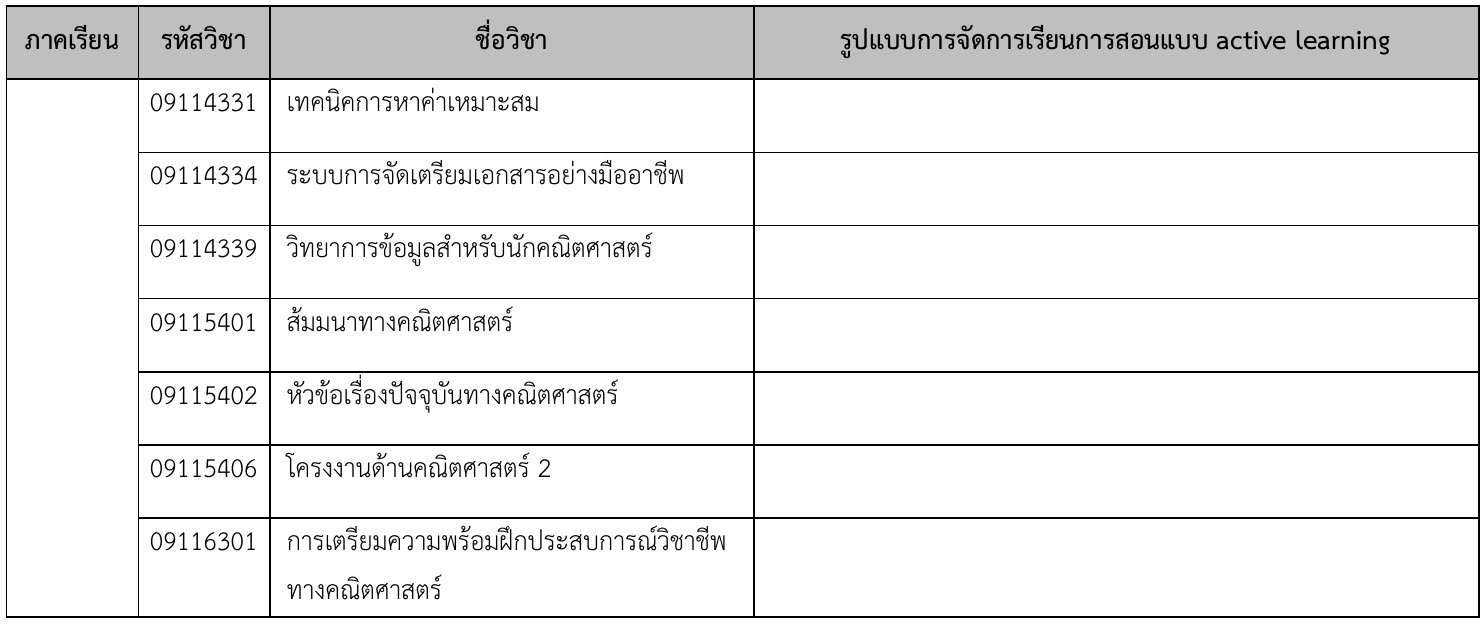
\includegraphics[width=1.05\textwidth]{Table3.3-2.jpg}
%\end{figure}
%\end{center}

\begin{doclist}
	\docitem{มคอ.3 }
	%\docitem{รูปแบบของการจัดการเรียนการสอนแบบ active learning ของแต่ละรายวิชาในหลักสูตร}
\end{doclist}


\subcriteria{The teaching and learning activities are shown to promote learning, learning how to learn, and instilling in students a commitment for life-long learning (e.g., commitment to critical inquiry, information-processing skills, and a willingness to experiment with new ideas and practices).}

เนื่องจากการสอนด้วยวิธีการ Active Learning จะทำ ให้ผู้เรียนเกิดแรงจูงใจในการเรียนรู้มากขึ้น  โดยผู้สอน
เป็นผู้อำนวยความสะดวก แนะนำ ช่วยเหลือสนับสนุนการเรียนรู้ ส่งผลทำให้เกิดบรรยกาศการเรียนการสอนที่ดีขึ้น ช่วยให้
ผู้เรียนเข้าใจบทเรียน สนใจ และเพิ่มแรงจูงใจให้กับผู้เรียนในการเรียนรู้ 
ดังนั้นหลักสูตรจึงส่งเสริมให้ทุกรายวิชามีการจัดการเรียนการสอนแบบ Active Learning เพื่อเป็นการสนับสนุนการเรียนรู้ให้กับนักศึกษา

หลักสูตรมีการส่งเสริมการเรียนรู้ตลอดชีวิต (life-long learning) ให้กับนักศึกษาในด้าน ทักษะการสืบค้นข้อมูล ความเป็นผู้นำ และการทำงานเป็นทีม โดยหลักสูตรฯ กำหนดให้ทุกรายวิชามีการส่งเสริมการเรียนรู้ตลอดชีวิตในด้านดังกล่าวให้กับนักศึกษา

%%%%%%%%%%%%%%




\begin{doclist}
	\docitem{มคอ.3 ของแต่ละรายแต่รายวิชา}
	\docitem{รายงานการประชุมอาจารย์ผู้รับผิดชอบหลักสูตร/อาจารย์ประจำสาขาวิชา การจัดการเรียนการสอนรายวิชาสัมมนา และการกำหนด Life-Long Learning ของหลักสูตร}
\end{doclist}


\subcriteria{The teaching and learning activities are shown to inculcate in students, new ideas, creative thought, innovation, and an entrepreneurial mindset.}

หลักสูตรมีการจัดกิจกรรมการเรียนการสอนเพื่อปลูกฝังให้ผู้เรียนมีความคิดใหม่ ๆ มีความคิดสร้างสรรค์ และมีแนวคิดการสร้างนวัตกรรม เช่น รายวิชาโครงงาน รายวิชาอัตลักษณ์แห่งราชมงคลธัญบุรี รายวิชา การคิดเชิงออกแบบ และรายวิชาสหกิจศึกษา เป็นต้น

หลักสูตรส่งเสริมแนวคิดการเป็นผู้ประกอบการ โดยจัดให้นักศึกษาเรียนรายวิชา 00-100-301 ความเป็นผู้ประกอบการ ซึ่งเป็นรายวิชาที่ศึกษาเกี่ยวกับแนวโน้มและแนวคิดในการทำธุรกิจ การเป็นผู้ประกอบการ การจัดการองค์กร การตลาด การจัดการด้านการเงิน การเป็นผู้ประกอบการที่ประสบความสำเร็จ การจัดทำแบบจำลองธุรกิจ
 
\begin{doclist}
	\docitem{ตัวอย่าง มคอ.3 รายวิชาที่ส่งเสริมแนวคิดการสร้างนวัตกรรมและแนวคิดความเป็นผู้ประกอบการ}
\end{doclist}

\subcriteria{The teaching and learning processes are shown to be continuously improved to ensure their relevance to the needs of industry and are aligned to the expected learning outcomes.}

หลักสูตรมีการปรับปรุงกระบวนการและกลยุทธ์การจัดการเรียนการสอนอย่างต่อเนื่องเพื่อให้แน่ใจว่ามีความสอดคล้องกับความต้องการของอุตสาหกรรมหรือสถานประกอบการและสอดคล้องกับผลการเรียนรู้ที่คาดหวัง โดยหลักสูตรได้ส่ง มคอ.3 รายวิชาระเบียบวิธีเชิงตัวเลขเบื้องต้นและรายวิชาระบบฐานข้อมูล ให้ผู้เชี่ยวชาญจากภาคอุตสาหกรรมให้ข้อเสนอแนะเกี่ยวกับกิจกรรมการเรียนการสอนในรายวิชาดังกล่าว โดยมีข้อเสนอแนะคือ หลักสูตรควรเพิ่มกิจกรรมการเรียนการสอนแบบเน้นปฏิบัติ ควรมีการนำกรณีศึกษาและปัญหาจากสถานประกอบ ให้นักศึกษาได้แก้ปัญหาจริง หรือควรเชิญผู้เชี่ยวชาญจากสถานประกอบการมาให้ความรู้ เพื่อให้เห็นความเชื่อมโยงระหว่างเนื้อหาที่เรียนในห้องเรียนกับการนำไปใช้จริงในสถานประกอบการ 

ผู้สอนในรายวิชาาระเบียบวิธีเชิงตัวเลขเบื้องต้นและรายวิชาระบบฐานข้อมูลได้นำข้อเสนอแนะมาปรับปรุงกิจกรรมการเรียนการสอนโดยมีการจัดกิจกรรมการเรียนการสอนแบบ Active Learning ในบางหัวข้อ และได้เชิญผู้เชี่ยวชาญจากสถานประกอบการคือ นายจิรพัฒน์ ลิ้มธนกุล ตำแหน่ง Senior Engineer Western Digital Storage Technology (Thailand) มาให้ความรู้ในหัวข้อ Python for industrial and application ในรายวิชาระเบียบวิธีเชิงตัวเลขเบื้องต้นและรายวิชาระบบฐานข้อมูล 




\begin{doclist}
	\docitem{มคอ.3 รายวิชาระเบียบวิธีเชิงตัวเลขเบื้องต้นและรายวิชาระบบฐานข้อมูล}
	\docitem{ภาพกิจกรรมการบรรยายหัวข้อ Python for industrial and application}
\end{doclist}


\newpage
\criteria{Student Assessment}
%%%%%%% 4.1 %%%%%%%%%%%%%%%%%%%%%%%
\subcriteria{A variety of assessment methods are shown to be used and are shown to be constructively aligned to achieving the expected learning outcomes and the teaching and learning objectives.}

ในปีการศึกษา 2567 ทุกรายวิชาของหลักสูตรมีวิธีการประเมินผลผู้เรียนที่หลากหลายและสอดคล้องกับผลลัพธ์การเรียนรู้ระดับรายวิชา (CLOs) ของรายวิชา เพื่อให้ผู้เรียนบรรลุผลลัพธ์การเรียนรู้ระดับหลักสูตร (PLOs) ซึ่งปรากฎในรายละเอียดของรายวิชา (มคอ.3) หมวดที่ 4 ในที่นี้จะแสดงตัวอย่างการประเมินผลผู้เรียนของรายวิชา 09-111-151 แคลคูลัส 1 ซึ่งรายวิชานี้รับผิดชอบการบรรลุ PLOs ของหลักสูตรจำนวน 3 PLOs ดังนี้
\begin{enumerate}[leftmargin=2.5cm]
	\item[PLO2:]อธิบายบทนิยาม หลักการและทฤษฎีบททางด้านคณิตศาสตร์และวิทยาศาสตร์ที่สำคัญได้อย่าง\\ถูกต้อง
	\item[PLO3:]คำนวณเพื่อแก้ปัญหาทางด้านคณิตศาสตร์ ตามหลักการ บทนิยาม และทฤษฎีบทได้อย่างถูกต้องเหมาะสม
	\item[PLO5:]ประยุกต์ใช้ความรู้ ทักษะ และเทคโนโลยีทางคณิตศาสตร์ในการแก้ปัญหาทางด้านวิทยาศาสตร์ วิศวกรรมศาสตร์ ธุรกิจอุตสาหกรรม หรือศาสตร์ที่เกี่ยวข้อง
\end{enumerate}
โดยมีผลลัพธ์การเรียนรู้ระดับรายวิชา (CLOs) ที่ผลักดันการบรรลุผลลัพธ์การเรียนรู้ระดับหลักสูตร (PLOs) ดังตาราง \ref{table: clos_cal1} และมีวิธีการสอนและวิธีการประเมินผลผู้เรียน ดังตาราง \ref{table:Cal1-2}
\begin{longtable}{|>{\centering\raggedright}p{0.44\textwidth}|>{\centering\raggedright}p{0.28\textwidth}|>{\centering}p{0.05\textwidth}|>{\centering}p{0.05\textwidth}|>{\centering\arraybackslash}p{0.05\textwidth}|}
	\caption{ความเชื่อมโยงระหว่างผลลัพธ์การเรียนรู้ระดับรายวิชา (CLOs) ของรายวิชา 09-111-151 แคลคูลัส 1 กับผลลัพธ์การเรียนรู้ระดับหลักสูตร (PLOs)}
	\label{table: clos_cal1}
	\\
	\hline
	\centering\textbf{คำอธิบายรายวิชา} & \centering\textbf{CLOs} & \multicolumn{3}{c|}{\textbf{PLOs}}\\ \cline{3-5}
	& & 2 & 3 & 5 \\ \hline
	\endfirsthead
	\caption{(ต่อ) ความเชื่อมโยงระหว่างผลลัพธ์การเรียนรู้ระดับรายวิชา (CLOs) ของรายวิชา 09-111-151 แคลคูลัส 1 กับผลลัพธ์การเรียนรู้ระดับหลักสูตร (PLOs) }
	\\
	\hline
	\textbf{คำอธิบายรายวิชา} & \textbf{CLOs} & \multicolumn{3}{c|}{\textbf{PLOs}}\\ \cline{3-5}
	& & 2 & 3 & 5 \\ \hline
	\endhead
	\hline
	\endfoot
	\vspace{-0.4cm}
	\multirow{3}{0.45\textwidth}{ฟังก์ชันค่าจริงตัวแปรเดียว ลิมิตและความต่อเนื่องของฟังก์ชัน อนุพันธ์ของฟังก์ชันพีชคณิตและฟังก์ชันอดิศัย กฎลูกโซ่ อนุพันธ์โดยปริยาย อนุพันธ์อันดับสูง ทฤษฎีบทของโรล ทฤษฎีบทค่ามัชฌิม การประยุกต์ของอนุพันธ์อย่างง่าย ผลต่างเชิงอนุพันธ์ ปฏิยานุพันธ์ ปริพันธ์ไม่จำกัดเขต การหาปริพันธ์เบื้องต้น การหาปริพันธ์โดยการเปลี่ยนตัวแปร ผลบวกรีมันน์ ปริพันธ์จำกัดเขต ทฤษฎีบทหลักมูลของแคลคูลัส}&CLO1: อธิบายบทนิยามและทฤษฎีบทที่สำคัญเกี่ยวกับลิมิต ความต่อเนื่อง อนุพันธ์และปริพันธ์ของฟังก์ชันค่าจริงหนึ่งตัวแปรได้ & \checkmark& &\\ \cline{2-5}
	& CLO2: คำนวณลิมิต อนุพันธ์ ปริพันธ์และตรวจสอบความต่อเนื่องของฟังก์ชันค่าจริงหนึ่งตัวแปรได้& & \checkmark&  \\ \cline{2-5}
	& CLO3: ประยุกต์ใช้อนุพันธ์และปริพันธ์จำกัดเขตในการแก้ปัญหาได้ & & & \checkmark \\ \end{longtable}
%%%%%%%%%%%%%%%%%%%%%%%%%%%%%%%%%%%%%%%%%%
\begin{longtable}{| >{\raggedright}p{0.4\textwidth} | >{\raggedright}p{0.18\textwidth} | >{\raggedright}p{0.17\textwidth} | >{\centering\arraybackslash}p{0.1\textwidth} |}
	\caption{วิธีการสอนและการประเมินผลเพื่อให้บรรลุผลลัพธ์การเรียนรู้ระดับรายวิชา (CLOs) ของรายวิชา 09-111-151 แคลคูลัส 1}
	\label{table:Cal1-2}
	\\
	\hline
	\centering\textbf{CLOs} & \centering\textbf{วิธีการสอน} & \centering\textbf{วิธีการประเมินผล} & \textbf{สัดส่วนของการประเมิน}\\
	\hline
	\endfirsthead
			\caption{(ต่อ) วิธีการสอนและการประเมินผลเพื่อให้บรรลุผลลัพธ์การเรียนรู้ระดับรายวิชา (CLOs) ของรายวิชา 09-111-151 แคลคูลัส 1 }\\
			\hline
			\textbf{CLOs} & \textbf{วิธีการสอน} & \textbf{วิธีการประเมินผล } & \textbf{สัดส่วนของการประเมิน}\\
	\endhead
	\vspace{-0.6cm}	\begin{enumerate}[leftmargin=1.3cm]
		\item [CLO1:]อธิบายบทนิยามและทฤษฎีบทที่สำคัญเกี่ยวกับลิมิต ความต่อเนื่อง อนุพันธ์และปริพันธ์ของฟังก์ชันค่าจริงหนึ่งตัวแปรได้ 
		\end{enumerate}
			  
			&\vspace{-0.5cm}\begin{enumerate}[label=-,noitemsep]
				\item บรรยาย 
				\item อภิปราย
				\end{enumerate}
		& สอบข้อเขียน (Summative)
				 & 26\%\\
			\hline	
		\vspace{-0.6cm}	\begin{enumerate}[leftmargin=1.3cm]
			\item [CLO2:]คำนวณลิมิต อนุพันธ์ ปริพันธ์และตรวจสอบความต่อเนื่องของฟังก์ชันค่าจริงหนึ่งตัวแปรได้ 
		\end{enumerate}	
			& \vspace{-0.5cm}	\begin{enumerate}[label=-,noitemsep]
			\item บรรยาย 
			\item อภิปราย
		\end{enumerate}&สอบข้อเขียน (Summative)& 60\%\\
			\hline
			\vspace{-0.6cm}	\begin{enumerate}[leftmargin=1.3cm]
			\item [CLO3:]ประยุกต์ใช้อนุพันธ์และปริพันธ์จำกัดเขตในการแก้ปัญหาได้
		\end{enumerate}	
		& \vspace{-0.5cm}	\begin{enumerate}[label=-,noitemsep]
				\item บรรยาย 
				\item อภิปราย
				\item มอบหมายงาน
			\end{enumerate}
		&\vspace{-0.6cm}	\begin{enumerate}[label=-,noitemsep]
			\item สอบข้อเขียน (Summative)
			\item การนำเสนอ (Summative)
			\end{enumerate}& 14\%\\
		\hline
\end{longtable}

\begin{doclist}
	\docitem{รายละเอียดของรายวิชา (มคอ.3)}
	\docitem{รายงานผลการดำเนินการของรายวิชา (มคอ.5)}
\end{doclist}

%%%%%%% 4.2 %%%%%%%%%%%%%%%%%%%%%%%
\subcriteria{The assessment and assessment-appeal policies are shown to be explicit, communicated to students, and applied consistently.}
หลักสูตรมีนโยบายการวัดผลประเมินผลและการอุทธรณ์ผลการประเมินของทุกรายวิชา และมีการสื่อสารไปยังผู้เรียนอย่างสม่ำเสมอโดยแจ้งให้นักศึกษาทราบในคาบเรียนแรกของการเรียนการสอน ก่อนการสอบ และหลังการสอบ 

สำหรับการอุทธรณ์ผลการประเมินนักศึกษาสามารถดาวน์โหลดแบบฟอร์มได้จากเว็บไซต์\\ https://www.sci.rmutt.ac.th/student/ \\
\begin{figure}[h!]
		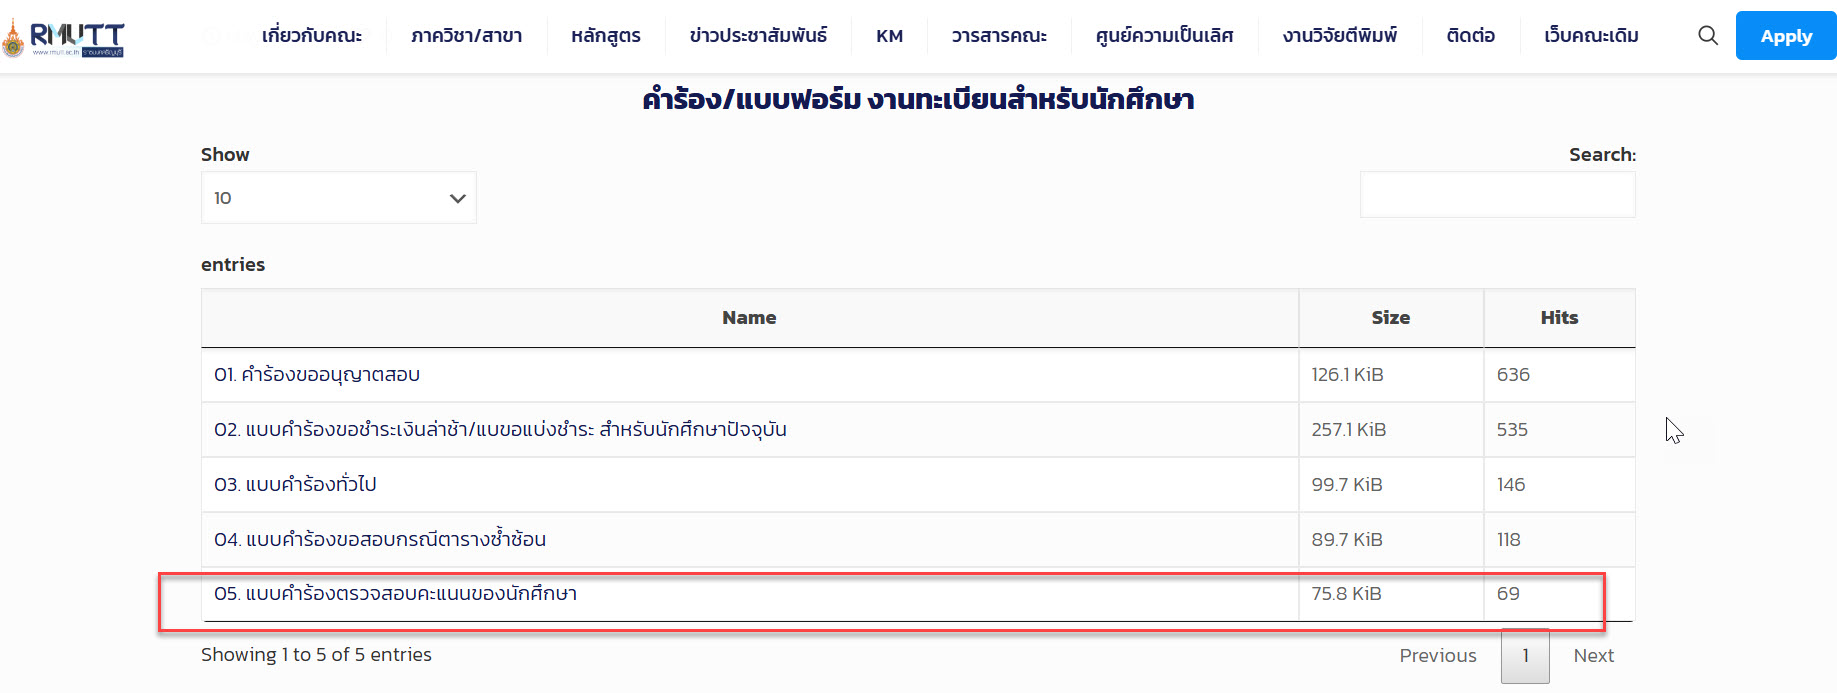
\includegraphics[width=\textwidth]{Pic4.2-2.jpg}
		\caption{เว็บไซต์สำหรับดาวน์โหลดเอกสารข้อร้องเรียนหรืออุทธรณ์ผลการประเมิน}
\end{figure}
\\
\noindent
\newpage
ขั้นตอนการอุทธรณ์ผลการประเมิน
\begin{enumerate}
\item ยื่นคำร้องที่เจ้าหน้าที่ธุรการสาขาในวันและเวลาราชการ โดยวันสุดท้ายที่จะสามารถยื่นเรื่องได้จะต้องไม่เกิน 7 วันทำการนับจากวันสุดท้ายที่คณะส่งค่าระดับคะแนนตามกำหนดการของสำนักส่งเสริมวิชาการและงานทะเบียน (สวท.)
\item ขอดูได้เป็นรายบุคคลเท่านั้น โดยธุรการสาขานัดหมายนักศึกษาให้มาดูเอกสารประกอบการตรวจสอบหลังจากยื่นคำร้องในวันทำการถัดไปในกรณีที่ยื่นคำร้องก่อนเวลา 12.00 น. หรือในอีก 2 วันทำการถัดไปในกรณีที่ยื่นคำร้องหลังเวลา 12.00 น.
\item ธุรการสาขาประสานงานกับคณะกรรมการการอุทธรณ์ที่ได้รับการแต่งตั้งจากสาขาวิชา ซึ่งคณะกรรมการชุดดังกล่าวไม่มีส่วนเกี่ยวข้องกับอาจารย์ผู้สอนรายวิชาที่นักศึกษาได้ยื่นเรื่องอุทธรณ์ เพื่อจัดเตรียมเอกสารและนัดหมายเวลาสำหรับการเข้าตรวจสอบคะแนนของนักศึกษา ทั้งนี้ให้ธุรการสาขาดำเนินการหลังจากได้รับคำร้องจากนักศึกษาทันที
\item ผู้สอนจัดเตรียมกระดาษคำตอบของนักศึกษาที่ยื่นคำร้อง เฉลย และเกณฑ์การให้คะแนนของข้อสอบในรายวิชา
นั้น ๆ ให้แก่คณะกรรมการการอุทธรณ์ที่ได้รับการแต่งตั้งจากสาขาวิชา
\item นักศึกษาเข้าพบธุรการสาขา และคณะกรรมการการอุทธรณ์ที่ได้รับการแต่งตั้งจากสาขาวิชาเพื่อตรวจสอบเอกสาร โดยไม่อนุญาตให้จด บันทึกภาพถ่ายหรือวีดีโอขณะทำการตรวจสอบเอกสาร
\item หากนักศึกษาไม่ยอมรับผลคะแนนสอบหลังจากทำการตรวจสอบคะแนนแล้ว ให้ธุรการสาขาส่งเรื่องต่อ
ให้กับงานทะเบียนและวัดผล ฝ่ายวิชาการ เพื่อดำเนินการแต่งตั้งคณะกรรมการเพื่อตรวจสอบการให้คะแนนของ
ผู้สอนอีกครั้ง โดยมีคณะกรรมการในการดำเนินการ 3 ท่าน คือ
\begin{enumerate}[label=\arabic*),leftmargin=1cm]
\item รองคณบดีฝ่ายวิชาการ 
\item หัวหน้างานทะเบียนและวัดผล
\item หัวหน้าภาควิชา/สาขาวิชา หรือตัวแทนคณะกรรมการหลักสูตรที่เกี่ยวข้อง
\end{enumerate}
\item งานทะเบียนและวัดผล ฝ่ายวิชาการ ดำเนินการนัดหมายคณะกรรมการในการตรวจสอบ อาจารย์ผู้สอนนักศึกษา และธุรการสาขา เพื่อดำเนินการตรวจสอบต่อไป และดำเนินการให้เสร็จสิ้นภายใน 3 วันทำการ
\end{enumerate}
ผลการดำเนินการในปีการศึกษา 2567 พบว่าไม่มีนักศึกษาดำเนินการอุทธรณ์ผลการประเมิน 

\begin{doclist}
	\docitem{แบบคำร้องขอตรวจสอบคะแนนของนักศึกษา}
\end{doclist}


%%%%%%% 4.3 %%%%%%%%%%%%%%%%%%%%%%%
\subcriteria{The assessment standards and procedures for student progression and degree completion, are shown to be explicit, communicated to students, and applied consistently.}
หลักสูตรได้กำหนดกระบวนการในการติดตามการประเมินผลและการสำเร็จการศึกษาของนักศึกษาไว้อย่างเป็นระบบและชัดเจน โดยยึดตามข้อบังคับของมหาวิทยาลัยเทคโนโลยีราชมงคลธัญบุรี ว่าด้วยการศึกษาระดับปริญญาตรี พ.ศ. 2556 และเป็นไปตามกรอบมาตรฐานคุณวุฒิระดับอุดมศึกษาแห่งชาติ (TQF) เพื่อให้มั่นใจว่าบัณฑิตทุกคนมีคุณภาพและเป็นไปตามผลลัพธ์การเรียนรู้ระดับหลักสูตร (PLOs) ของหลักสูตร ดังรายละเอียดต่อไปนี้ 
\begin{enumerate}
	\item หลักสูตรแต่งตั้งอาจารย์ที่ปรึกษาสำหรับดูแลนักศึกษาแต่ละชั้นปี ในการกำกับติดตามเกี่ยวกับ
	\begin{enumerate}[label=\arabic*),leftmargin=0.7cm]
		\item ด้านการลงทะเบียนเรียน
		\begin{itemize}
			\item ในภาคการศึกษาปกตินักศึกษาต้องลงทะเบียนเรียนไม่ต่ำกว่า 9 หน่วยกิต และไม่เกิน 22 หน่วยกิต สำหรับภาคฤดูร้อน นักศึกษาจะลงทะเบียนได้ไม่เกิน 9 หน่วยกิต หากไม่เป็นไปตามเกณฑ์นี้ให้ขออนุมัติต่อคณบดี และทำได้เพียง 1 ภาคการศึกษาเท่านั้นในการศึกษาตลอดหลักสูตร
			\item รายวิชาที่ลงทะเบียนในแต่ละภาคเรียนต้องเป็นไปตามแผนการศึกษา ในกรณีที่นักศึกษามีผลการเรียนไม่ถึง 2.00 นักศึกษาจะต้องได้รับการปลดล็อคและรับคำปรึกษาจากอาจารย์ที่ปรึกษาในการลงทะเบียนเรียน
			\item สำหรับนักศึกษาที่ต้องลงทะเบียนเรียนไม่เป็นไปตามแผนการเศึกษาที่กำหนด อาจารย์ที่ปรึกษาจะให้คำแนะนำปรึกษาการวางแผนลงทะเบียนเรียนและกำกับติดตามให้นักศึกษาลงทะเบียนเรียนรายวิชาให้ครบตามแผนการศึกษาของหลักสูตร
		\end{itemize}
		\item ด้านผลการศึกษา\\
		อาจารย์ที่ปรึกษากำกับติดตามผลการเรียนของนักศึกษาผ่านระบบงานทะเบียนทางเว็บไซต์ (www.oreg.rmutt.ac.th) เพื่อ
		\begin{itemize}
			\item ดูแนวโน้มผลการเรียนและแนะนำในการวางแผนการศึกษา
			\item เฝ้าระวังการพ้นสภาพตามเกณฑ์ ซึ่งมีเกณฑ์การพ้นสภาพดังนี้\\
			
			\begin{tabular}{|c|c|}
				\hline
				\textbf{หน่วยกิตสะสม}& \textbf{พ้นสภาพเมื่อได้ระดับคะแนน}\\\hline
				น้อยกว่า 30 หน่วยกิต& น้อยกว่า 1.00\\\hline
				30-59 หน่วยกิต& น้อยกว่า 1.50\\\hline
				60 หน่วยกิตขึ้นไป &  น้อยกว่า 1.75\\\hline
				ครบหลักสูตร &  น้อยกว่า 1.90\\\hline
			\end{tabular}\\
			หมายเหตุ รายวิชาที่ลงทะเบียนเรียนซ้ำ ให้นับหน่วยกิตเฉพาะที่ได้ระดับคะแนนดีที่สุดเพียงครั้งเดียว และการนับหน่วยกิตสะสมสำหรับเกณฑ์การพ้นสภาพเนื่องจากผลการศึกษาให้นับหน่วยกิตทุกรายวิชาที่ได้ค่าระดับคะแนน ยกเว้น W I S และ U
		\end{itemize}
		\item ด้านการสำเร็จการศึกษาตามหลักสูตร
		\begin{itemize}
			\item ต้องศึกษารายวิชาให้ครบตามโครงสร้างหลักสูตร
			\item มีจำนวนหน่วยกิตสะสมไม่ต่ำกว่า 137 หน่วยกิต และได้ค่าระดับคะแนนเฉลี่ยสะสมไม่ต่ำกว่า 2.00 จากระบบ 4 ระดับคะแนนหรือเทียบเท่า
			\item ใช้ระยะเวลาไม่เกิน 2 เท่าของระยะเวลาการศึกษาที่กำหนดไว้ในหลักสูตร ทั้งนี้ไม่นับระยะเวลาการลาพักการศึกษาด้วย
			\item มีผลการทดสอบภาษาอังกฤษเป็นไปตามเกณฑ์ที่มหาวิทยาลัยกำหนด
			\item มีคุณสมบัติอื่น ๆ ตามข้อบังคับของมหาวิทยาลัยเทคโนโลยีราชมงคลธัญบุรี ว่าด้วยการศึกษาระดับปริญญาตรี พ.ศ. 2550 และฉบับเพิ่มเติม พ.ศ. 2556
		\end{itemize}
	\end{enumerate}	
	\item หลักสูตรมีการสื่อสารให้นักศึกษาทราบถึงเกณฑ์การประเมินผลและการสำเร็จการศึกษาอย่างสม่ำเสมอผ่านช่องทาง ดังนี้
	\begin{itemize}
		\item การปฐมนิเทศนักศึกษาใหม่\\อาจารย์ที่ปรึกษาและคณาจารย์ในหลักสูตรฯ จะชี้แจงภาพรวมของหลักสูตร เกณฑ์การวัดผลและประเมินผล และเงื่อนไขการสำเร็จการศึกษาให้นักศึกษาใหม่ทราบทุกปีการศึกษา
		\item ระบบงานทะเบียน\\ นักศึกษาสามารถเข้าถึงรายละเอียดหลักสูตร ข้อบังคับต่างๆ และตรวจสอบผลการเรียนของตนเองได้ตลอดเวลาผ่านทางเว็บไซต์ของระบบงานทะเบียน (www.oreg.rmutt.ac.th)
		\item อาจารย์ที่ปรึกษา\\ให้คำแนะนำ ดูแล และให้คำปรึกษาแก่นักศึกษาในเรื่องการวางแผนการเรียนและติดตามผลการเรียนอย่างสม่ำเสมอ
	\end{itemize}
\end{enumerate}

\begin{doclist}
	\docitem{หลักสูตรวิทยาศาสตรบัณฑิต สาขาวิชาคณิตศาสตร์ประยุกต์ (หลัก\newline สูตรปรับปรุง พ.ศ. 2564)}
	\docitem{ข้อบังคับ ระเบียบ และประกาศ ที่เกี่ยวข้องกับการจัดการศึกษาของมหาวิทยาลัยเทคโนโลยีราชมงคลธัญบุรี}
	\docitem{คู่มือนักศึกษา}
\end{doclist}

%%%%%%% 4.4 %%%%%%%%%%%%%%%%%%%%%%%
\subcriteria{The assessments methods are shown to include rubrics, marking schemes, timelines, and regulations, and these are shown to ensure validity, reliability, and fairness in assessment.}
%%%%%%%%%%%%%%%%%%%%%%%%%%%%%%%%%%
เพื่อให้เกิดความมั่นใจว่าการวัดและประเมินผลนักศึกษามีความถูกต้อง เชื่อถือได้ และเป็นธรรม หลักสูตรมี​การดำเนินการดังนี้
\begin{enumerate}
\item ทุกรายวิชามีการแจ้งรายละเอียดของรายวิชา (มคอ.3) ซึ่งมีรายละเอียดของกำหนดการและเกณฑ์ในการวัดและประเมินผลของรายวิชาให้นักศึกษาทราบและแจกประมวลรายวิชา (Course Syllabus) ของรายวิชาที่มี Qr-code ของ มคอ.3 ให้กับนักศึกษาในคาบแรกของการเรียนการสอน
\item นักศึกษาทุกคนที่ลงทะเบียนเรียนในรายวิชา จะได้รับการประเมินผลการเรียนในรูปแบบ วิธีการ และเกณฑ์เดียวกัน
\item ข้อสอบสำหรับการประเมินผลในแต่ละรายวิชา อาจารย์ผู้สอนในรายวิชาเป็นผู้ออกข้อสอบ ในกรณีที่มีผู้สอนร่วมกัน อาจารย์ผู้สอนจะออกข้อสอบร่วมกันพร้อมทั้งตรวจสอบความถูกต้องของข้อสอบ สำหรับการตรวจข้อสอบแบบอัตนัย อาจารย์ผู้สอนจะทำแนวเฉลยข้อสอบหรือ marking schemes เพื่อให้อาจารย์ผู้สอนทุกท่านนำไปเป็นแนวทางในการตรวจข้อสอบ ดังตัวอย่าง marking schemes ของข้อสอบรายวิชาแคลคูลัส 1 (
รูปภาพที่ \ref{Picture:Marking Schemes})
\begin{figure}[h!]
	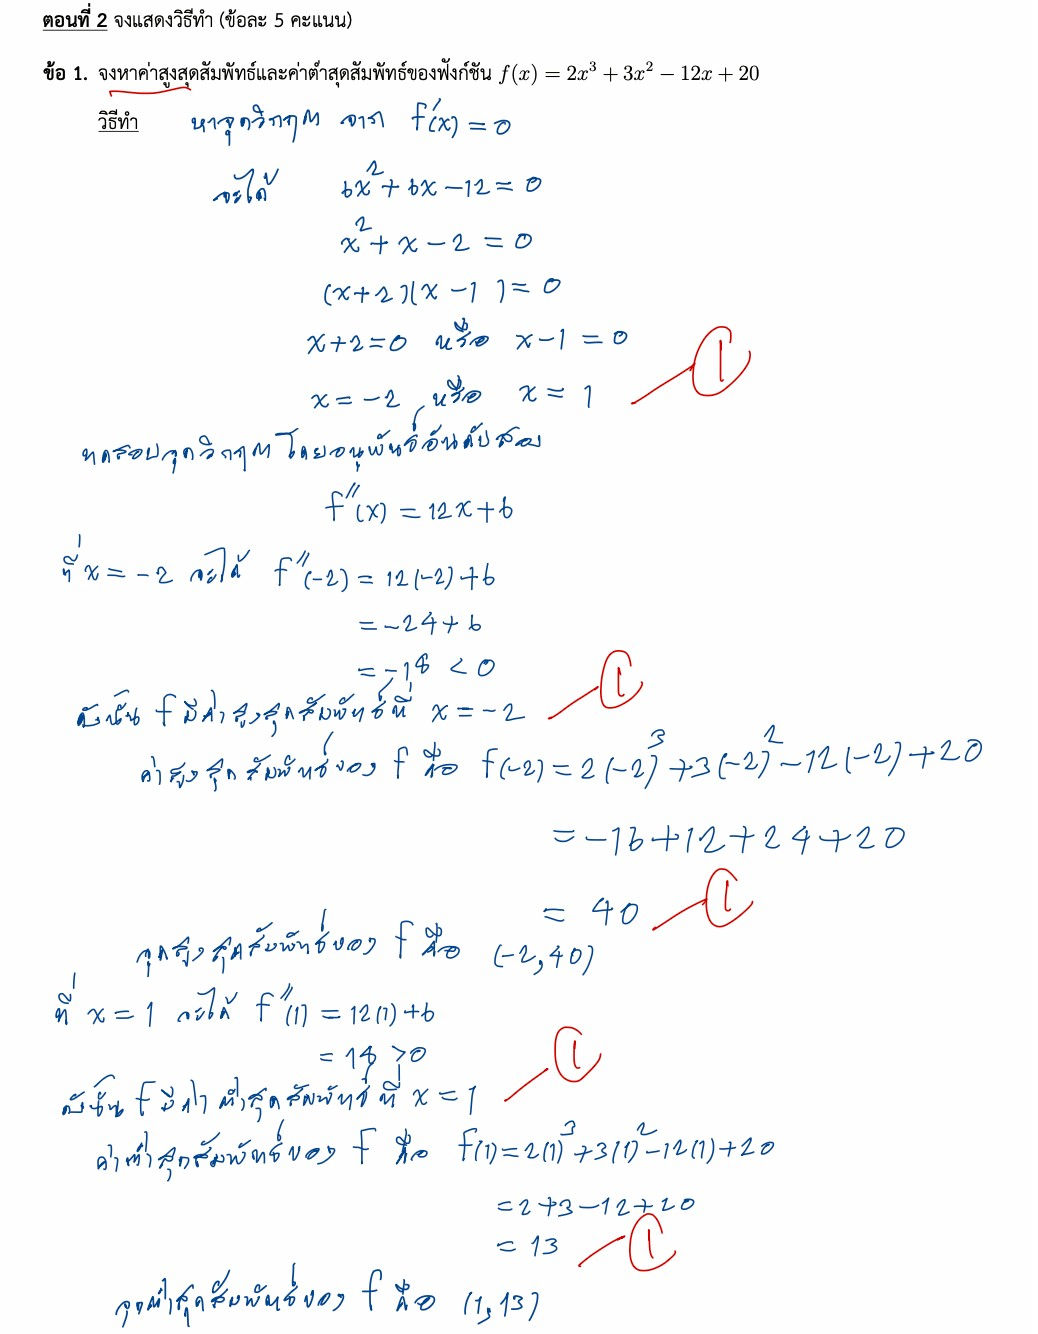
\includegraphics[width=\textwidth]{Calculus Points}\\
	\caption{ตัวอย่าง Marking Schemes ของข้อสอบรายวิชา Calculus 1}
	\label{Picture:Marking Schemes}
\end{figure}
\item สำหรับรายวิชาชีพที่มีการประเมินผลการนำเสนอผลงาน ผู้สอนมีการจัดทำ Scoring Rubrics สำหรับให้คะแนนทุกรายวิชาดังตาราง \ref{table: Scoring Rubrics}

\renewcommand{\arraystretch}{1.5} % เพิ่มความสูงบรรทัดให้อ่านง่ายขึ้น

\begin{longtable}{|p{3cm}|p{1.8cm}|p{1.8cm}|p{1.8cm}|p{1.8cm}|p{1.8cm}|p{1cm}|}
		\caption{เกณฑ์การให้คะแนน (Scoring Rubrics) สำหรับการประเมินผลการนำเสนอ}
	\label{table: Scoring Rubrics}\\
	\hline
	\centering\textbf{รายการประเมิน}&\multicolumn{5}{c|}{\textbf{ระดับคะแนน}}&\textbf{คะแนน\newline ที่ได้}\\ \cline{2-6}
	& \centering\textbf{5} & \centering\textbf{4} & \centering\textbf{3} & \centering\textbf{2} & \centering\textbf{1} &  \\
	\hline
	\endfirsthead
	
	\caption{(ต่อ) เกณฑ์การให้คะแนน (Scoring Rubrics) สำหรับการประเมินผลการนำเสนอ }\\
	\hline
\centering\textbf{รายการประเมิน}&\multicolumn{5}{c|}{\textbf{ระดับคะแนน}}&\textbf{คะแนน\newline ที่ได้}\\ \cline{2-6}
& \centering\textbf{5} & \centering\textbf{4} & \centering\textbf{3} & \centering\textbf{2} & \centering\textbf{1} &  \\
\hline
	\endhead
					\vspace{-0.55cm}
	\begin{itemize}
		\item[1.]ความถูกต้อง \newline ของเนื้อหา \newline (30\%) 
	\end{itemize}
 & 
	ข้อมูลถูกต้อง\newline ครบถ้วน \newline น่าเชื่อถือสูง \newline อ้างอิง\newline ได้ชัดเจน &
	ข้อมูลถูกต้อง น่าเชื่อถือ อ้างอิงได้  &
	ข้อมูลถูกต้องเป็นส่วนใหญ่ มีข้อผิดพลาดเล็กน้อย &
	ข้อมูลมี\newline ข้อผิดพลาดหลายจุด \newline ไม่น่าเชื่อถือบางส่วน&
	ข้อมูลมี\newline ข้อผิดพลาดอย่างมาก \newline ไม่น่าเชื่อถือ&
	\\
	\hline
				\vspace{-0.55cm}
	\begin{itemize}
		\item[2.]การนำเสนอ \newline(20\%)
	\end{itemize}
	& 
	การนำเสนอมีความน่าสนใจอย่างยิ่ง\newline สามารถดึงดูดความสนใจของ\newline ผู้ชมได้อย่างยอดเยี่ยม &
	การนำเสนอมีความน่าสนใจ\newline ดึงดูดความสนใจของ\newline ผู้ชมได้ดี &
	การนำเสนอค่อนข้าง\newline น่าเบื่อ\newline ไม่สามารถดึงดูดความสนใจได้ตลอด&
	การนำเสนอไม่น่าสนใจ ไม่ดึงดูดผู้ชม &
	การนำเสนอไม่น่าสนใจและไม่ดึงดูดผู้ชมเลย &
	\\
	\hline
			\vspace{-0.55cm}
	\begin{itemize}
		\item[3.]การใช้สื่อ\newline ประกอบ\newline(15 \%)
	\end{itemize}
  &
	อธิบายและเชื่อมโยงสื่อประกอบ\newline กับการ\newline นำเสนอได้อย่างกลมกลืน ช่วยให้ผู้ชมเข้าใจเนื้อหาได้ดียิ่งขึ้น &
	อธิบายและเชื่อมโยงสื่อประกอบกับการนำเสนอได้ดี &
	อธิบายสื่อประกอบบ้าง แต่ยังไม่เชื่อมโยงกับการ\newline นำเสนอ &
	ไม่มีการอธิบาย \newline หรืออธิบายสื่อประกอบได้ไม่ดี &
	ไม่มีการอธิบาย \newline หรืออธิบายสื่อประกอบได้ไม่ดีเลย &
	 \\
	\hline
		\vspace{-0.55cm}
	\begin{itemize}
		\item[4.]การตอบคำถาม\newline ข้อซักถาม\newline (30\%)
	\end{itemize}
 &
	ตอบคำถามได้อย่างยอดเยี่ยม มั่นใจ\newline มีเหตุผลประกอบที่ดี และสามารถจัดการกับ\newline คำถามยากๆ ได้ &
ตอบคำถามได้ดี มั่นใจ \newline และมีเหตุผลประกอบ &
	ตอบคำถามได้บ้าง แต่ยัง\newline ไม่มั่นใจ หรือใช้เวลานาน &
	ไม่สามารถตอบคำถามได้ หรือตอบ\newline ผิด &
	ไม่สามารถตอบคำถามได้เลย \newline หรือตอบผิดทั้งหมด &
\\
	\hline
	\vspace{-0.55cm}
	\begin{itemize}
		\item[5.]การบริหารเวลา\newline(5\%)
	\end{itemize}
	&
	บริหารเวลาได้อย่างยอดเยี่ยมนำเสนอได้ครบถ้วนตามเวลาที่กำหนด และมีเวลาสำหรับตอบคำถาม  \newline ได้อย่างเหมาะสม &
	บริหารเวลาได้ดี นำเสนอได้ตามเวลาที่กำหนด &
	ใช้เวลาพอดี แต่บางส่วนรีบเร่ง หรือใช้เวลากับบางประเด็นมากเกินไป &
	ใช้เวลา \newline ไม่เหมาะสม น้อยเกินไป หรือเกินเวลามาก &
ใช้เวลา \newline ไม่เหมาะสม  \newline อย่างมาก น้อยเกินไป หรือเกินเวลามากเกินไป &
	\\
	\hline
	
\end{longtable}


\item การแจ้งผลการเรียนของรายวิชาหลังเสร็จสิ้นภาคการศึกษา อาจารย์ผู้สอนเป็นผู้รวบรวมคะแนนของนักศึกษาและจัดทำเกรดตามเกณฑ์ที่กำหนดไว้ใน มคอ.3 และนำเสนอต่อที่ประชุมสาขาวิชาคณิตศาสตร์เพื่อพิจารณา หลังจากนั้นนำเข้าสู่การพิจารณาโดยคณะกรรมการบริหารคณะและคณะกรรมการประจำคณะ หากผ่านการพิจารณาของคณะกรรมการบริหารคณะและคณะกรรมการประจำคณะ ไม่มีปัญหาใด อาจารย์ผู้รับผิดชอบในการ submit เกรดของสาขาวิชา จะดำเนินการ submit เกรดของนักศึกษาทุกรายวิชา ผ่านระบบ OREG ของมหาวิทยาลัย

\end{enumerate}
%%%%%%%%%%%%%%%%%%%%%%%%%%%%%%%%%%%%
\begin{doclist}
	\docitem{Marking Schemes ของข้อสอบรายวิชา Calculus 1 }
	\docitem{Scoring Rubrics สำหรับการประเมินผลการนำเสนอ}
\end{doclist}



%%%%%%% 4.5 %%%%%%%%%%%%%%%%%%%%%%%
\subcriteria{The assessment methods are shown to measure the achievement of the expected learning outcomes of the programme and its courses.}
%%%%%%%%%%%%%%%%%%%%%%%%%%%%%%%5
หลักสูตรมีวิธีการวัดและประเมินการบรรลุความสำเร็จตามผลลัพธ์การเรียนรู้ระดับรายวิชา (CLOs) และผลลัพธ์การเรียนรู้ระดับหลักสูตร (PLOs) ดังนี้
\begin{enumerate}
	\item วิธีการวัดและประเมินผลการบรรลุผลลัพธ์การเรียนรู้ระดับรายวิชา (CLOs)
	\begin{itemize}
		\item[1)] การประเมินผลโดยผู้สอน ผ่านการวัดผลของรายวิชา
		\item[2)] การประเมินตนเองของนักศึกษา โดยให้นักศึกษาทำแบบประเมินการบรรลุ CLOs เมื่อสิ้นภาคการศึกษา
	\end{itemize}
	\item วิธีการวัดและประเมินผลการบรรลุผลลัพธ์การเรียนรู้ระดับหลักสูตร (PLOs)
	\begin{itemize}
		\item[1)] การประเมินผลโดยตรงผ่านผลงานและการวัดผลในชั้นเรียนโดยผู้สอนของทุกรายวิชาที่รับผิดชอบการบรรลุแต่ละ PLOs 
		\item[2)] การประเมินตนเองของนักศึกษาชั้นปีที่ 4 ผ่านแบบประเมินการบรรลุ PLOs เมื่อสิ้นภาคการศึกษา 2/\printyear{} 
		\item[3)] การประเมินความพึงพอใจของผู้ใช้บัณฑิตซึ่งเป็นมุมมองสะท้อนกลับจากผู้มีส่วนได้ส่วนเสียภายนอก
	\end{itemize}
	ซึ่งมีรายละเอียดและผลการประเมินดัง criterion 1.5
\end{enumerate}
\begin{doclist}
	\docitem{ผลการประเมินการบรรลุผลลัพธ์การเรียนรู้ระดับหลักสูตร (PLOs)}
	\docitem{ผลการประเมินการบรรลุผลลัพธ์การเรียนรู้ระดับรายวิชา (CLOs)}
\end{doclist}

%%%%%%% 4.6 %%%%%%%%%%%%%%%%%%%%%%%
\subcriteria{Feedback of student assessment is shown to be provided in a timely manner.}

หลักสูตรมีนโยบายให้ผู้สอนในทุกรายวิชาดำเนินการให้ข้อมูลย้อนกลับ (Feedback) แก่นักศึกษาอย่างสม่ำเสมอ ภายหลังการประเมินผล เพื่อให้นักศึกษาได้รับข้อมูลที่ชัดเจนเกี่ยวกับผลการเรียน จุดแข็ง จุดที่ควรปรับปรุง และแนวทางการพัฒนาในครั้งต่อไป โดยมีรูปแบบการดำเนินการที่สำคัญ ดังนี้
\begin{enumerate}
	\item  อาจารย์ผู้สอนทุกรายวิชามีการแจ้งผลการประเมิน และให้ข้อมูลย้อนกลับ (Feedback) แก่นักศึกษา
	\begin{itemize}
		\item คะแนนสอบกลางภาค/คะแนนทดสอบย่อย\\
		มีการเฉลยแบบทดสอบ ให้ข้อเสนอแนะ ข้อควรปรับปรุง เพื่อปรับปรุงพัฒนาตนเอง เตรียมพร้อมสำหรับการสอบในครั้งถัดไป หรือวางแผนถอนรายวิชา
		\item คะแนนชิ้นงาน \\มีการให้ข้อเสนอแนะข้อควรปรับปรุง เพื่อพัฒนาชิ้นงาน
		\item คะแนนการนำเสนอ \\มีการให้ข้อเสนอแนะข้อควรปรับปรุงในการนำเสนอ
	\end{itemize} 
	\item การให้ข้อมูลย้อนกลับในรายวิชาโครงงานด้านคณิตศาสตร์ประยุกต์\\
นักศึกษาจะได้รับข้อมูลย้อนกลับจากอาจารย์อย่างต่อเนื่อง ทั้งในระหว่างการดำเนินโครงงานและหลังการนำเสนอ โดยเฉพาะข้อเสนอแนะเพื่อพัฒนาแนวคิด วิธีการและผลลัพธ์ของโครงงาน
	\item การให้ข้อมูลย้อนกลับในรายวิชาสัมมนาทางคณิตศาสตร์ประยุกต์\\
ในรายวิชาสัมมนาทางคณิตศาสตร์ หลักสูตรได้จัดให้มีคณะกรรมการประเมินการนำเสนอการถอดบทเรียนและอาจารย์ที่ปรึกษา เพื่อให้คำแนะนำเชิงวิชาการและข้อเสนอแนะเฉพาะบุคคลระหว่างการนำเสนอของนักศึกษา โดยกรรมการจะมีการสอบถาม วิเคราะห์ และเสนอแนวทางพัฒนาอย่างเป็นระบบ เพื่อใหนักศึกษาสามารถนำ feedback ที่ได้รับไปปรับปรุงในการนำเสนอครั้งถัดไป
	\end{enumerate}


%%%%%%% 4.7 %%%%%%%%%%%%%%%%%%%%%%%
\subcriteria{The student assessment and its processes are shown to be continuously reviewed and improved to ensure their relevance to the needs of industry and alignment to the expected learning outcomes.}

หลักสูตรมีการทบทวนกลไกการวัดและประเมินผลการเรียนรู้ของนักศึกษาอย่างต่อเนื่องโดยมุ่งเน้นให้การวัดและประเมินผลมีความสอดคล้องกับผลลัพธ์การเรียนรู้ระดับรายวิชา (CLOs) วัตถุประสงค์ของรายวิชา และความต้องการของภาคอุตสาหกรรมในปัจจุบัน โดย 
\begin{enumerate}
	\item เก็บรวบรวมข้อมูลข้อเสนอแนะจากอาจารย์ผู้สอน \\ โดยอาจารย์ผู้สอนให้ข้อเสนอแนะในการปรับปรุงการประเมินผลไว้ใน มคอ.5 หลังจากนั้นอาจารย์ผู้รับผิดชอบรายวิชาและอาจารย์ผู้สอนประชุมร่วมกัน
	เพื่อพิจารณาข้อเสนอแนะและนำมาใช้ในการปรับปรุงการวัดและประเมินผลในภาคเรียนถัดไป
	\item เก็บรวบรวมข้อเสนอแนะจากนักศึกษา\\ โดยอาจารย์ผู้สอนรวบรวมข้อมูลเสนอแนะจากนักศึกษาเมื่อสิ้นภาคการศึกษา ในกรณีที่นักศึกษามีข้อเสนอแนะเพิ่มเติมเกี่ยวกับการวัดและประเมินผล หลักจากนั้นอาจารย์ผู้สอนนำข้อเสนอแนะที่เป็นประโยชน์เสนอต่อที่ประชุมอาจารย์ผู้สอนและผู้รับผิดชอบรายวิชา เพื่อเป็นข้อมูลในการปรับปรุงการประเมินผลรายวิชาในภาคการศึกษาถัดไป
	\item การทวนสอบฯ\\
	หลักสูตรมีการทวนสอบผลสัมฤทธิ์ของนักศึกษาตามผลลัพธ์การเรียนรู้ระดับรายวิชา (CLOs) ของทุกรายวิชาชีพที่เปิดสอนในแต่ละภาคเรียน โดย
	\begin{itemize}
		\item แต่งตั้งคณะกรรมการทวนสอบฯ
		\item คณะกรรมการทวนสอบฯ ดำเนินการทวนสอบหลังสิ้นภาคเรียน
		\item คณะกรรมการทวนสอบฯ รายงานผลการทวนสอบให้หลักสูตรทราบ และแจ้งผลการทวนสอบพร้อมทั้งข้อเสนอแนะให้กับอาจารย์ผู้รับผิดชอบรายวิชา และอาจารย์ผู้สอนทราบเพื่อนำไปปรับปรุงการวัดและประเมินผลในภาคการศึกษาถัดไป
	\end{itemize}
	\item เก็บข้อมูลข้อเสนอแนะจากภาคอุตสาหกรรม\\
	ในแต่ละปีการศึกษา หลักสูตรมีการเก็บรวบรวมข้อมูลข้อเสนอแนะจากภาคอุตสาหกรรมจากหลายช่องทาง เช่น การสัมภาษณ์สถานประกอบการที่นักศึกษาออกฝึกประสบการวิชาชีพ ข้อเสนอแนะจากผู้ทรงคุณวุฒิจากหน่วยงานภายนอกที่มาร่วมพิจารณาเกรดในการประชุมคณะกรรมการประจำคณะ
\end{enumerate}

ในปีการศึกษา 2567  มีรายวิชาที่เปิดสอนในหลักสูตรจำนวน 31 รายวิชา แบ่งเป็น
\begin{enumerate}
	\item[] - ภาคเรียนที่ 1/2567 จำนวน 11 รายวิชา
	\item[] - ภาคเรียนที่ 2/2567 จำนวน 20 รายวิชา
\end{enumerate}
พบว่าทุกรายวิชามีการออกแบบการวัดและการประเมินผลที่สอดคล้องกับผลลัพธ์การเรียนรู้ระดับรายวิชา (CLOs) นอกจากนี้ จากการสัมภาษณ์สถานประกอบการที่นักศึกษาออกฝึกประสบการณ์วิชาชีพ ในภาคเรียนที่ 1 ปีการศึกษา 2567 ทางสถานประกอบการมีข้อเสนอแนะว่าหลักสูตรควรเพิ่มการประเมินผลในลักษณะที่นักศึกษาได้เลือกสถานการณ์ของปัญหา เลือกวิธีวิเคราะห์และแก้ปัญหาด้วยตนเอง พร้อมทั้งนำเสนอแนวคิดและวิธีการแก้ปัญหานั้นๆ เพื่อส่งเสริมให้นักศึกษาได้ฝึกคิดวิเคราะห์และนำเสนอ และเตรียมพร้อมสำหรับการปฏิบัติงานจริงในสถานประกอบการ ที่ต้องมีการคิดการวิเคราะห์และการนำเสนองานในส่วนที่ตนเองรับผิดชอบอยู่เสมอ ซึ่งถือเป็นทักษะที่สำคัญมากในการทำงานที่ทางสถานศึกษาควรส่งเสริม

หลักสูตรได้นำข้อเสนอแนะมาปรับปรุงการดำเนินงานในภาคเรียนที่ 2/2567 ในรายวิชาการตัดสินใจอย่างชาญฉลาดด้วยกำหนดการเชิงคณิตศาสตร์ โดยเพิ่มกิจกรรมการประเมินผลตามข้อเสนอแนะจากสถานประกอบการ โดยเปิดโอกาสให้นักศึกษาเลือกปัญหาที่เป็นไปได้จากสถานการณ์จริง และออกแบบวิธีการแก้ปัญหาด้วยตนเองพร้อมนำเสนอ




\begin{doclist}
	\docitem{รายงานผลการทวนสอบปีการศึกษา 2567}
	\docitem{หลักฐานการปรับปรุงการประเมินผลรายวิชาการตัดสินใจอย่างชาญฉลาดด้วยกำหนดการเชิงคณิตศาสตร์}
\end{doclist}



\newpage
\criteria{Academic Staff}
%%%%%%%%%% 5.1 %%%%%%%%%%%%%%%
\subcriteria{The programme to show that academic staff planning (including succession, promotion, 
	re-deployment, termination, and retirement plans) is carried out to ensure that the quality and quantity of the academic staff fulfil the needs for education, research, and service.
}

เพื่อให้หลักสูตรมีอาจารย์ผู้รับผิดชอบหลักสูตรมีบุคลากรที่มีคุณภาพและปริมาณที่เพียงพอต่อการจัดการเรียนการสอน การวิจัย และการบริการทางวิชาการ หลักสูตรฯ มีการวางแผนเกี่ยวกับการรับและการแต่งตั้งอาจารย์ผู้รับผิดชอบหลักสูตรวิทยาศาสตร์บัณฑิต สาขาวิชาคณิตศาสตร์ประยุกต์ (หลักสูตรปรับปรุง พ.ศ. 2564) โดยมีขั้นตอน/กระบวนการในการดำเนินงานเกี่ยวกับการรับและการแต่งตั้งอาจารย์ผู้รับผิดชอบหลักสูตร ดังนี้
\begin{enumerate} 
\item กำหนดคุณสมบัติของอาจารย์ผู้รับผิดชอบหลักสูตร 
\begin{itemize} 
\item มีคุณสมบัติตามเกณฑ์มาตรฐานหลักสูตรระดับปริญญาตรี (พ.ศ. 2565)   
\item มีงานวิจัยตีพิมพ์อย่างต่อเนื่อง ย้อนหลัง 5 ปี 
\item มีตำแหน่งทางวิชาการ/อยู่ระหว่างการเสนอขอตำแหน่งทางวิชาการ หรือมีอายุราชการไม่น้อยกว่า 5 ปี  
\item มีความเชี่ยวชาญทางด้านคณิตศาสตร์ประยุกต์ที่สอดคล้องกับหลักสูตร 
\end{itemize} 
\item คัดเลือกอาจารย์ผู้รับผิดชอบหลักสูตรจากอาจารย์ผู้สอนในสาขาวิชาฯ 
\item หลักสูตรดำเนินการแต่งตั้งอาจารย์ผู้รับผิดชอบหลักสูตรตามขั้นตอนที่มหาวิทยาลัยกำหนด 
\end{enumerate}

 ในปีการศึกษา 2566 หลักสูตรมีอาจารย์ผู้สอน และอาจารย์ผู้รับผิดชอบหลักสูตรรวมทั้งสิ้น 18 คน โดยมีอาจารย์ผู้สอนจำนวน 13 คน ลาศึกษาต่อจำนวน 1 คน จะเกษียณอายุราชการในปีการศึกษา 2569 จำนวน 1 คน และมีอาจารย์ผู้รับผิดชอบหลักสูตรจำนวน 5 คน จะเกษียณอายุราชการในปีการศึกษา 2570 จำนวน 1 คน 
 
\begin{longtable}{|l|c|}
	\caption{ตารางแสดงปีที่เกษียณอายุราชการของอาจารย์ผู้รับผิดชอบหลักสูตร}
	\\
	\hline
	\textbf{อาจารย์ผู้รับผิดชอบหลักสูตร} & \textbf{ปีที่เกษียณอายุราชการ}\\
	\hline
	1. ผศ.สมนึก ศรีสวัสดิ์ & 2570\\
	2. รศ.ดร.พงศกร สุนทรายุทธ์  &2589 \\ 
	3. ผศ.ดร.วงศ์วิศรุต เขื่องสตุ่ง & 2591\\
	4. ดร.รัฐพรหม พรหมคำ  &2588 \\
	5. ผศ.มงคล ทาทอง & 2581\\
	\hline
\end{longtable}
\newpage
\begin{longtable}{|l|c|}
	\caption{ตารางแสดงปีที่เกษียณอายุราชการของอาจารย์ผู้สอน}
	\\
	\hline
	\textbf{อาจารย์ผู้สอน} & \textbf{ปีที่เกษียณอายุราชการ}\\
	\hline
	1. ผศ.กุลประภา ศรีหมุด 	& 2580 \\
	2. ผศ.ดร.กมลรัตน์ สมบุตร 	&2587\\
	3. ผศ.ดร.ภคีตา สุขประเสริฐ	& 2588\\
	4. ผศ.ดร.ปริญญวัฒน์ ชูสุวรรณ &2592 \\
	5. ดร.วรรณา ศรีปราชญ์	& 2578\\
	6. ดร.นนธิยา มากะเต	& 2580\\
	7. อ.อลงกต สุวรรณมณี	& 2584\\
	8. อ.โอม สถิตยนาค	& 2586\\
	9. อ.วาสนา ทองกำแหง	& 2581\\
	10. อ.อัคเรศ สิงห์ทา	& 2580\\
	11. อ.อมราภรณ์ บำเพ็ญดี	& 2580\\
	12. อ.ธาวัลย์ อัมพวา	& 2569\\
	13. ดร.ปฤณท์ธพร สงวนสุทธิกุล	& 2595\\
	\hline
\end{longtable}

 สำหรับแผนในการขออัตรากำลังทดแทนอาจารย์ผู้รับผิดชอบหลักสูตรและอาจารย์ผู้สอน ทางหลักสูตรจะดำเนินการร่วมกับคณะในลำดับต่อไป


\begin{doclist}
	\docitem{แผนกรอบอัตรากำลังของคณะ}
\end{doclist}
%%%%%%%%%% 5.2 %%%%%%%%%%%%%%%
\subcriteria{The program to show that staff workload is measured and monitored to improve the quality of education, research, and service.}
มหาวิทยาลัยกำหนดอัตราส่วนอาจารย์ต่อนักศึกษาเต็มเวลาระดับปริญญาตรีเท่ากับ 1:20 เพื่อให้
อาจารย์สามารถดูแลนักศึกษาได้อย่างทั่วถึง ตามการประกันคุณภาพการศึกษา ซึ่งในปีการศึกษา 2566 หลักสูตรมี
อาจารย์ประจำหลักสูตรที่ปฏิบัติงานจริงทั้งสิ้น 17 คน และมีจำนวนนักศึกษาเต็มเวลาที่ทางหลักสูตรให้บริการสอน(วิชาชีพ และวิชาศึกษาทั่วไป) จำนวน 366.53 คิดเป็นสัดส่วนของอาจารย์ต่อนักศึกษาเต็มเวลาเท่ากับ 17 : 366.53 หรือ 1 : 21.56 ดังตาราง \ref{table: FTE} ซึ่งถือว่าสัดส่วนของอาจารย์ต่อนักศึกษาแตกต่างจากเกณฑ์ที่มหาวิทยาลัยกำหนดเพียงเล็กน้อย ถือได้ว่าหลักสูตรมีคุณภาพด้านการดูแลนักศึกษา

\begin{landscape}
	\centering
	\begin{longtable}{|p{0.07\textwidth}|p{0.08\textwidth}|p{0.07\textwidth}|p{0.07\textwidth}|p{0.09\textwidth}|p{0.07\textwidth}|p{0.07\textwidth}|p{0.1\textwidth}|p{0.1\textwidth}|p{0.1\textwidth}|p{0.09\textwidth}|p{0.07\textwidth}|p{0.07\textwidth}|p{0.09\textwidth}|}
		\caption{อัตราส่วนอาจารย์ผู้สอนในหลักสูตรต่อนักศึกษา}
		\label{table: FTE}
		\\
		\hline
		\multirow{2}{0.1\textwidth}{\textbf{ปีการศึกษา}} & \multirow{2}{0.1\textwidth}{\textbf{จำนวนอาจารย์ผู้สอนในหลักสูตร (A)}} & \multicolumn{3}{c|}{\textbf{ศึกษาทั่วไป+วิชาชีพ}} & \multicolumn{3}{c|}{\textbf{วิชาชีพ}}  & \multicolumn{3}{c|}{\textbf{วิชาชีพพื้นฐานที่ต้องสอนให้หลักสูตรอื่น}}  &\multicolumn{3}{c|}{\textbf{รายวิชาศึกษาทั่วไป}}\\
		\cline{3-14}
		& &FTE ของอาจารย์รวม (B) & FTES ของนักศึกษา (C)& อัตราส่วนของนักศึกษาต่ออาจารย์ {\tiny $(D)=\dfrac{(C)}{(A)}$} &FTE ของอาจารย์รวม (B) & FTES ของนักศึกษา (C)& อัตราส่วนของนักศึกษาต่ออาจารย์ {\tiny $(D)=\dfrac{(C)}{(A)}$} &FTE \newline ของอาจารย์รวม (B) & FTES ของนักศึกษา (C)& อัตราส่วนของนักศึกษาต่ออาจารย์ {\tiny $(D)=\dfrac{(C)}{(A)}$} &FTE ของอาจารย์รวม (B) & FTES ของนักศึกษา (C)& อัตราส่วนของนักศึกษาต่ออาจารย์ {\tiny $(D)=\dfrac{(C)}{(A)}$}\\
		\hline
		2564&18&17.6&441.81&24.55&4.25&29.56&1.64&12.45&388.5&21.58&0.9&23.75&1.32\\
		\hline
		2565&18&16&356.86&19.83&4.56&33.69&1.87&10.39&292.42&16.25&1.05&30.75&1.71\\
		\hline
		2566&17&21.15&366.53&21.56&5.62&40.69&2.39&11.49&297.08&17.48&4.05&28.75&1.69\\
		\hline
	\end{longtable}
\end{landscape}

เมื่อพิจารณาข้อมูลภาระงานและสัดส่วนของอาจารย์ต่อนักศึกษาเต็มเวลาเทียบเท่าย้อนหลัง 3 ปี พบว่า มีค่าไม่แตกต่างกันมากนัก ทำให้บุคลากรสายวิชาการสามารถมีเวลาในการทำงานวิจัยและบริการทางวิชาการได้

\begin{doclist}
	\docitem{การคำนวณค่า FTE ของหลักสูตร ปีการศึกษา 2564-2566}
	\docitem{การคำนวณค่า FTES ของหลักสูตร ปีการศึกษา 2564-2566}
\end{doclist}

%%%%%%%%%% 5.3 %%%%%%%%%%%%%%%
\subcriteria{The programme to show that the competences of the academic staff are determined, evaluated, and communicated.}
หลักสูตรใช้เกณฑ์ของมหาวิทยาลัยและคณะในการกำหนดและประเมินสมรรถนะสำหรับบุคลากรสายวิชาการ ซึ่งการกำหนดหัวข้อการประเมินสมรรถนะและเกณฑ์การประเมินสำหรับบุคลากรสายวิชาการของคณะจะถูกจัดทำโดย คณะกรรมการฯ ผ่านความเห็นชอบจากคณะกรรมการบริหารและคณะกรรมการประจำคณะวิทยาศาสตร์และเทคโนโลยี
และมีการทำประชาพิจารณ์ร่วมกันระหว่างผู้บริหารและบุคลากรสายวิชาการก่อนนำแบบประเมินมาใช้โดยสมรรถนะที่ใช้ในการประเมินแบ่งเป็น 5 ด้านดังนี้
\begin{enumerate}
	\item งานสอน
	\item งานวิจัย สิ่งประดิษฐ์ นวัตกรรมและผลงานวิชาการ
	\item งานบริการวิชาการ
	\item งานด้านอื่นๆ หรืองานที่ได้รับมอบหมาย
	\item งานจัดหารายได้จากหน่วยงานภายนอก
\end{enumerate}
สมรรถนะแต่ละด้านจะมีค่าน้ำหนักแตกต่างกันไป รายละเอียดของข้อมูลแสดงดังภาพที่ \ref{Pic5.3-1}\\
\begin{figure}[h!]
	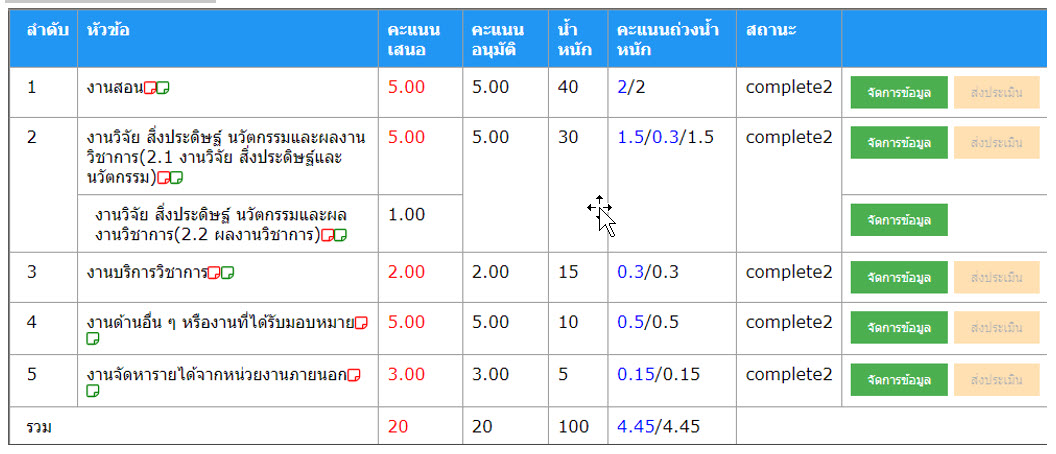
\includegraphics[width=\textwidth]{Pic5.3-1.jpg}
	\caption{ระบบประเมินสมรรถนะบุคลากรสายวิชาการ}
	\label{Pic5.3-1}
\end{figure}

โดยการประเมินสมรรถนะของบุคลากรจะอยู่ในรูปของการประเมินเพื่อเลื่อนขั้นเงินเดือนปีละ 2 ครั้ง ครั้งที่ 1 ประเมินสมรรถนะการปฏิบัติงานในช่วง 1 ตุลาคม ถึง 31 มีนาคม และครั้งที่ 2 ประเมินสมรรถนะการปฏิบัติงานในช่วง 1 เมษายน ถึง 30 กันยายน ผ่านระบบจัดการข้อมูลการประเมินบุคลากรคณะวิทยาศาสตร์และเทคโนโลยี 

นอกจากนั้นยังมีการประเมินสมรรถนะหลักของบุคลากรสายวิชาการที่กำหนดโดยมหาวิทยาลัย 6 ด้าน ประกอบไปด้วย
\begin{enumerate}
\item รักองค์กรและหน้าที่ มีจิตสำนึก ในการเป็นเจ้าของ เห็นคุณค่าองค์กร มุ่งมั่นการทำงานในหน้าที่
อย่างเป็นระบบ มีวินัยและคุณธรรมพัฒนาตนเอง และองค์กรไปสู่เป้าหมายอย่างต่อเนื่อง
\item พัฒนาตนเองเรียนรู้วิทยาการใหม่ๆ เพื่อพัฒนาและเพิ่มศักยภาพในการทำงาน ที่มีประสิทธิภาพ
และสอดคล้องต่อการ เปลี่ยนแปลง มีความรู้ ความเชี่ยวชาญ
\item เป็นมืออาชีพ มีความรู้ ความเชี่ยวชาญ ในการปฏิบัติงาน และเชื่อมโยง แก้ไขปัญหาในการทำงาน
ได้ อย่างเหมาะสมตามจรรยาบรรณวิชาชีพ
\item สื่อสารอย่างสร้างสรรค์ การถ่ายทอดข้อมูลข่าวสารโดยใช้สื่อต่างๆ มีการแลกเปลี่ยนความคิดเห็น 
และสร้างความเข้าใจร่วมกันในการทำงาน อย่างมีประสิทธิภาพเพื่อพัฒนางาน และองค์กร
\item ทำงานเป็นทีม เปิดใจกว้าง รับฟังความคิดเห็น เรียนรู้และแก้ไข ปัญหาร่วมกันอย่างมีประสิทธิภาพ 
เพื่อบรรลุเป้าหมายเดียวกัน
\item จิตสาธารณะตระหนักถึงประโยชน์ ส่วนรวมถ่ายทอดความรู้ประสบการณ์ ให้กับองค์กร สังคม
ชุมชน และประเทศชาติ
\end{enumerate}

โดยมีการกำหนดระดับสมรรถนะที่คาดหวัง ระดับสมรรถนะที่ผู้ถูกประเมินประเมินตนเอง และระดับสมรรถนะที่ประเมินโดยคณะกรรมการประเมิน ซึ่งมีคณะกรรมการ 2 ชุด คือ คณะกรรมการกลั่นกรองขั้นที่ 1 และคณะกรรมการประเมินชุดที่ 2 เป็นผู้ประเมิน รายละเอียดของข้อมูลแสดงดังภาพที่ \ref{Pic5.3-2}
\begin{figure}[h!]
	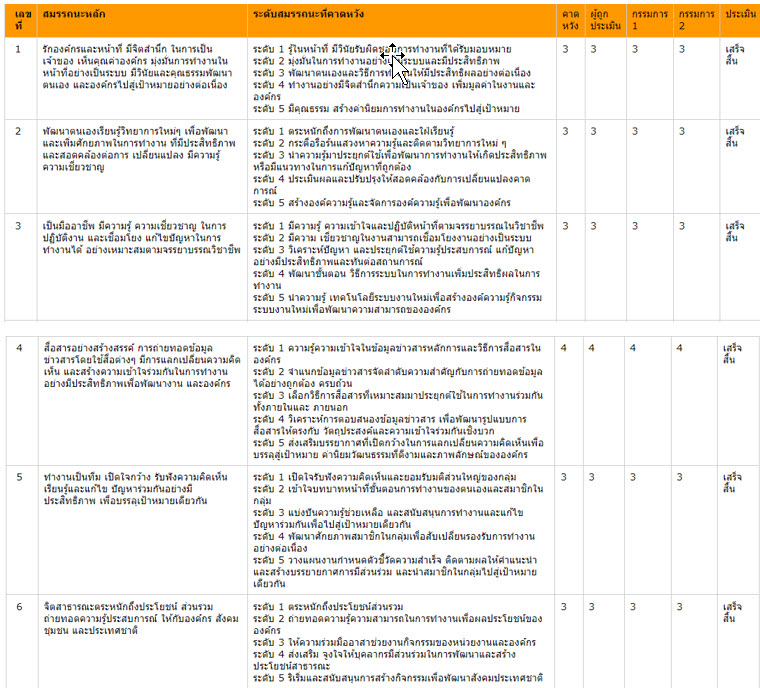
\includegraphics[width=\textwidth]{Pic5.3-2.jpg}
	\caption{สมรรถนะหลักของบุคลากรสายวิชาการที่กำหนดโดยมหาวิทยาลัย}
	\label{Pic5.3-2}
\end{figure}
รายละเอียดต่าง ๆ ในการเตรียมเอกสารและการ upload file จะมีการสื่อสารให้บุคลากรสายวิชาการได้รับทราบและเข้าใจตรงกันอย่างทั่วถึง โดยมีการสื่อสารจากการประชุมบุคลากรของคณะโดยคณบดี รองคณบดีฝ่ายบริหารและวางแผนเป็นผู้ชี้แจง ประชุมภาควิชาโดยหัวหน้าภาควิชาเป็นผู้ชี้แจง ประชุมสาขาวิชาโดยหัวหน้าสาขาวิชาเป็นผู้ชี้แจง กลุ่มบุคลากรสายวิชาการที่ถูกประเมินจะแบ่งเป็น 5 กลุ่มคือ 1) พนักงานมหาวิทยาลัยวุฒิปริญญาเอก 2) พนักงานมหาวิทยาลัยวุฒิปริญญาโท 3) ข้าราชการพลเรือน 4) ข้าราชการ (ที่เป็นผู้บริหาร) และ 5) พนักงานมหาวิทยาลัยวุฒิปริญญาเอก (ที่เป็นผู้บริหาร) นอกจากนั้นรายละเอียดการประเมินของบุคลากรสายวิชาการแต่ละกลุ่ม ขั้นตอนการประเมิน วิธีการ upload เอกสารเข้าสู่ระบบการประเมิน สามารถศึกษาคู่มือการใช้ระบบนี้ได้จากเว็บไซต์  https://sci1.rmutt.ac.th/?page\_id=22472  แสดงดังภาพที่ \ref{Pic5.3-3}\newpage

\begin{figure}[h!]
	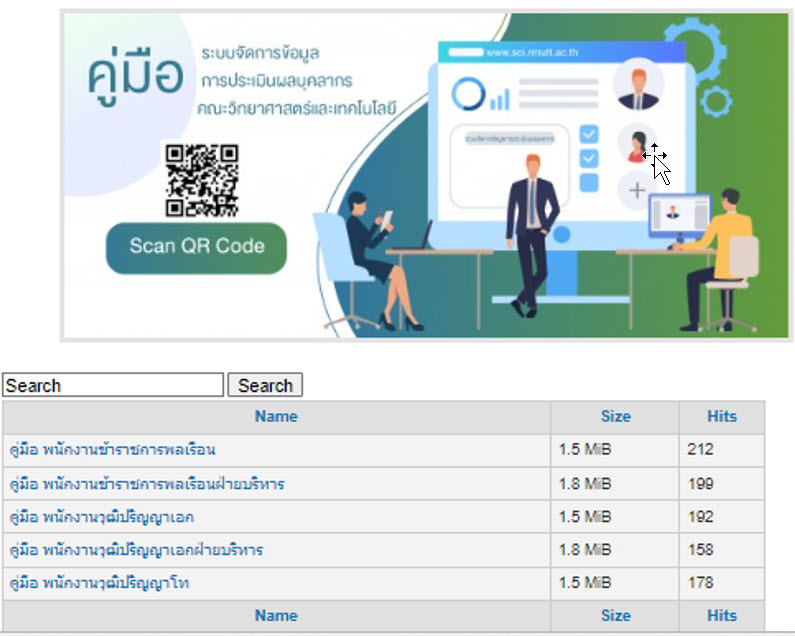
\includegraphics[width=\textwidth]{Pic5.3-3.jpg}
	\caption{คู่มือการใช้งานระบบจัดการข้อมูลการประเมินบุคลากรคณะวิทยาศาสตร์และเทคโนโลยี}
	\label{Pic5.3-3}
\end{figure}
\noindent
ขั้นตอนการประเมินสมรรถนะบุคลากรสายวิชาการ
\begin{enumerate}
\item ฝ่ายบริหารและวางแผนแจ้งบุคลากรสายวิชาการทราบถึงช่วงเวลาที่ จะต้อง upload เอกสารภาระงานตามสมรรถนะด้านต่าง ๆ ขึ้นสู่ระบบ 
\item บุคลากรสายวิชาการเตรียมเอกสารประเมินและ upload เอกสารเข้าสู่ระบบภายในเวลาที่กำหนด
\item คณะกรรมการประเมินชุดที่ 1 ที่เป็นคณะกรรมการกลั่นกรองเบื้องต้นประเมินเอกสาร 
\item คณะกรรมการเบื้องต้นแจ้ง ผลการประเมินเบื้องต้นกับบุคลากรสายวิชาการถึงคะแนนเบื้องต้น เอกสารหลักฐานครบถ้วนหรือไม่ หากเอกสารไม่ครบถ้วนมีการเปิดระบบให้ส่งเอกฐานเพิ่มเติม
\item คณะกรรมการประเมินชุดที่ 2 ประเมินผลการปฏิบัติงานต่อจากคณะกรรมการประเมินชุดที่ 1 หากมีข้อทักท้วงไม่เห็นด้วยให้ชี้แจงและส่งเอกสารแนบภายในระยะเวลาที่ระบบเปิดเท่านั้น
\item เอกสารผลการประเมินขั้นสุดท้ายส่งถึงผู้ถูกประเมิน เพื่อรับทราบและยอมรับผลการประเมิน
\end{enumerate}

ที่ผ่านมาในการประเมินผลการปฏิบัติงานของบุคลากรสายวิชาการ สาขาวิชาคณิตศาสตร์ประยุกต์ไม่มีปัญหาการฟ้องร้อง หรือการไม่ยอมรับผลการประเมิน เนื่องจากผลการประเมินยึดจากเอกสารหลักฐาน และผลการปฏิบัติงานซึ่งเป็นข้อเท็จจริงตามเกณฑ์การประเมินที่กำหนดไว้อย่างชัดเจน

\begin{doclist}
	\docitem{ระบบจัดการข้อมูลการประเมินบุคลากรคณะวิทยาศาสตร์และเทคโนโลยีออนไลน์}
\end{doclist}

%%%%%%%%%% 5.4 %%%%%%%%%%%%%%%
\subcriteria{The programme to show that the duties allocated to the academic staff are appropriate to qualifications, experience, and aptitude.}

บุคลากรสายวิชาการมีภาระหน้าที่หลัก คือ งานสอน วิจัย บริการวิชาการ และงานที่ได้รับมอบหมายทั้งในระดับสาขาวิชาและระดับคณะ 

การกำหนดผู้สอนของรายวิชา อาจารย์ผู้รับผิดชอบหลักสูตรจะพิจารณากำหนดผู้สอนรายวิชาตามความเชี่ยวชาญ ประสบการณ์การสอน ประสบการณ์การทำวิจัย โดยให้เป็นไปตามเกณฑ์ภาระงานขั้นต่ำ และกำหนดให้ผู้สอน 1 ท่าน มีจำนวนรายวิชาที่สอนไม่เกินภาคเรียนละ 3 รายวิชา

สำหรับการมอบหมายภาระงานในหลักสูตร จะพิจารณาจากความรู้ ความสามารถ ประสบการณ์ และความถนัดของอาจารย์แต่ละท่าน เช่น 
\begin{enumerate}
\item งานวิจัย มอบหมายให้ รศ.ดร.พงศกร สุนทรายุทธ์ และ ผศ.ดร.วงศ์วิศรุต เขื่องสตุ่ง เป็นผู้รับผิดชอบหลัก เนื่องจากมีประสบการณ์ในการวิจัย มีผลงานตีพิมพ์เป็นจำนวนมาก และมีประสบการณ์ในการเป็นหัวหน้าโครงการวิจัย
\item การบริหารหลักสูตร มอบหมายให้ ผศ.สมนึก ศรีสวัสดิ์ ผศ.มงคล ทาทอง ผศ.ดร.วงศ์วิศรุต เขื่องสตุ่ง รศ.ดร.พงศกร สุนทรายุทธ์ และ ดร.รัฐพรหม พรหมคำ เป็นผู้รับผิดชอบหลัก เนื่องจากเป็นอาจารย์ผู้รับผิดชอบหลักสูตร และมีประสบการณ์การบริหารหลักสูตร
\item การจัดหาสิ่งสนับสนุนการเรียนรู้ มอบหมายให้ ผศ.มงคล ทาทอง เป็นผู้รับผิดชอบหลัก เนื่องจากมีประสบการณ์ในการจัดซื้อจัดจ้าง การขอวัสดุครุภัณฑ์  
\item งานประกันคุณภาพการศึกษา มอบหมายให้ ผศ.สมนึก ศรีสวัสดิ์ ผศ.มงคล ทาทอง ผศ.ดร.วงศ์วิศรุต เขื่องสตุ่ง รศ.ดร.พงศกร สุนทรายุทธ์ และ ดร.รัฐพรหม พรหมคำ เป็นผู้รับผิดชอบหลัก เนื่องจากมีประสบการณ์การประกันคุณภาพหลักสูตร
\item งานบริการวิชาการ มอบหมายให้ ดร.รัฐพรหม พรหมคำ เป็นผู้รับผิดชอบหลัก เนื่องจากมีประสบการณ์ด้านการจัดโครงการการบริการวิชาการ
\end{enumerate}

โดยอาจารย์ผู้สอนในหลักสูตรท่านอื่น ๆ จะเป็นผู้ช่วยรับผิดชอบในแต่ละงาน และทำหน้าที่ตามพันธกิจหลักของอาจารย์ทั้ง 3 ด้านคือ สอน วิจัย และบริการวิชาการ

%%%%%%%%%% 5.5 %%%%%%%%%%%%%%%
\subcriteria{The programme to show that promotion of the academic staff is based on a merit system which accounts for teaching, research, and service.}

การขอกำหนดตำแหน่งทางวิชาการของบุคลากรสายวิชาการ มหาวิทยาลัยมีการกำหนด
ขั้นตอนการดำเนินงานการขอกำหนดตำแหน่งทางวิชาการของบุคลากรสายวิชาการ ดังนี้\\

\noindent
{\bf ส่วนของคณะ (การประเมินการสอน)}
\begin{enumerate}
\item ผู้ขอประเมินการสอน ยื่นเอกสารขอประเมินการสอน  งานบุคลากรตรวจสอบคุณสมบัติพร้อมเอกสาร
\item เสนอเรื่องไปยังคณบดี พร้อมเสนอชื่อคณะอนุกรรมการประเมินการสอน จำนวน 3 ท่าน โดย
คณะกรรมการประกอบไปด้วย \\1) คณบดี \\2) อาจารย์ในสาขาวิชาที่ขอตำแหน่งทางวิชาการ และ \\3) หัวหน้าภาควิชา/หัวหน้าสาขาวิชา
\item ตั้งอนุกรรมการประเมินการสอน 
\item นำส่งเอกสารและแบบฟอร์มการประเมินไปยังคณะอนุกรรมการประเมินการสอน
\item  รวบรวมผลการประเมินฯ ส่งมหาวิทยาลัย 
\end{enumerate}
ขั้นตอนการเสนอขอกำหนดตำแหน่งทางวิชาการ
\begin{enumerate}
\item คณะ/วิทยาลัย รับผลงานและเอกสารที่เกี่ยวข้องจากผู้เสนอขอกำหนดตำแหน่งทางวิชาการ โดยดำเนินการดังนี้
\begin{enumerate}[label=1.\arabic*,leftmargin=0.7cm, labelsep=2mm]
\item ตรวจสอบคุณสมบัติการขอกำหนดตำแหน่ง
\item ตรวจสอบเอกสารที่เกี่ยวข้องให้ครบถ้วน
\item แต่งตั้งคณะอนุกรรมการประเมินการสอนและประเมินเอกสารตามตำแหน่งทางวิชาการ
\item ดำเนินการให้คณะอนุกรรมการประเมินการสอนและประเมินเอกสารฯให้แล้วเสร็จและผ่าน
การประเมิน
\end{enumerate}
\item คณะ/วิทยาลัย ดำเนินการทำหนังสือส่งพร้อมรวบรวมผลงาน  เอกสารที่เกี่ยวข้อง คำสั่งแต่งตั้งอนุกรรมการ  ผลการประเมินการสอน ส่งกองบริหารงานบุคคล
\item กองบริหารงานบุคคลตรวจสอบคุณสมบัติ ผลงานทางวิชาการและเอกสารที่เกี่ยวข้อง ตามกรณีดังนี้
\begin{enumerate}[label=3.\arabic*,leftmargin=0.7cm, labelsep=2mm]
\item คุณสมบัติและผลงานไม่เป็นไปตามเกณฑ์ที่ ก.พ.อ.กำหนด ส่งเรื่องคืนคณะ/วิทยาลัย
\item เอกสารที่เกี่ยวข้องไม่ถูกต้อง ไม่ครบถ้วน แจ้งผู้เสนอขอให้นำกลับไปแก้ไข
\end{enumerate}
\item นำเข้าการประชุมคณะกรรมการกลั่นกรองผลงานทางวิชาการ เพื่อกลั่นกรองผลงานทางวิชาการเบื้องต้น
\item นำเข้าประชุมคณะกรรมการพิจารณาตำแหน่งทางวิชาการ เพื่อพิจารณาการเสนอขอและเลือกสรรผู้ทรงคุณวุฒิ ผู้ประเมินผลงานทางวิชาการ
\item ทาบทามผู้ทรงคุณวุฒิเพื่อทำหน้าที่ประเมินผลงานทางวิชาการจริยธรรมและจรรยาบรรณทางวิชาการ
\item ส่งผลงานให้ผู้ทรงคุณวุฒิประเมินผลงานทางวิชาการ
\item ประชุมคณะกรรมการผู้ทรงคุณวุฒิประเมินผลงานทางวิชาการเพื่อสรุปผลการประเมินผลงานทางวิชาการ
\item นำเข้าการประชุมคณะกรรมการพิจารณาตำแหน่งทางวิชาการ โดยหากมีมติปรับปรุงผลงาน ดำเนินการตามขั้นตอน ข้อที่ 9.1 - 9.3 หากไม่มีการปรับปรุงผลงานทำตามขั้นตอนข้อที่ 10
\begin{enumerate}[label=9.\arabic*,leftmargin=0.7cm, labelsep=2mm]
\item หากมีมติให้ปรับปรุงผลงาน กองบริหารงานบุคคลแจ้งต้นสังกัดให้ผู้เสนอขอฯปรับปรุงผลงาน 
ตามกำหนดเวลา
\item เมื่อผู้เสนอขอปรับปรุงผลงานแล้วเสร็จ กองบริหารงานบุคคลนำส่งผลงานปรับปรุงให้
ผู้ทรงคุณวุฒิประเมิน ผลงานปรับปรุง
\item เมื่อผู้ทรงคุณวุฒิฯประเมินผลงานปรับปรุงแล้วเสร็จ จึงนำเข้าการประชุมคณะกรรมการ
พิจารณาตำแหน่ง ทางวิชาการ
\end{enumerate}
\item นำเข้าการประชุมสภามหาวิทยาลัยเพื่อพิจารณาผลการขอกำหนดตำแหน่งทางวิชาการ
\item แจ้งผลการขอกำหนดตำแหน่งทางวิชาการไปยังต้นสังกัด โดยรอมติสภามหาวิทยาลัยเพื่อดำเนินการดังนี้
\begin{enumerate}[label=11.\arabic*,leftmargin=0.8cm, labelsep=2mm]
\item กรณีอนุมัติ ส่งคำสั่งแต่งตั้งและการ์ดแสดงความยินดีไปยังคณะ/
วิทยาลัย
\item กรณีไม่อนุมัติ แจ้งเรื่องและรายละเอียดการไม่อนุมัติไปยังคณะ/วิทยาลัย
\end{enumerate}
\end{enumerate}

 หลักสูตรมีกระบวนการส่งเสริมการเข้าสู่ตำแหน่งทางวิชาการโดยให้อาจารย์ทุกท่านจัดทำแผนการเสนอขอกำหนดตำแหน่งทางวิชาการ จัดระบบพี่เลี้ยงให้คำแนะนำปรึกษาและกำกับติดตาม ส่งผลให้
ในปีการศึกษา 2566 มีอาจารย์ผู้รับผิดชอบหลักสูตรเสนอขอกำหนดตำแหน่งทางวิชาการในตำแหน่งรองศาสตราจารย์ จำนวน 1 คน และตำแหน่งผู้ช่วยศาสตราจารย์ จำนวน 1 คน 
นอกจากนี้ยังมีอาจารย์ผู้สอนเสนอขอกำหนดตำแหน่งทางวิชาการ อีก 1 คน ปัจจุบันในหลักสูตร
มีอาจารย์ที่มีตำแหน่งทางวิชาการจำนวน 8 คน จาก 18 คน คิดเป็นร้อยละ 44.44 
\begin{doclist}
	\docitem{เว็บไซต์ของมหาวิทยาลัยที่ให้ข้อมูลเกี่ยวกับการเข้าสู่ตำแหน่งทางวิชาการ https://www.ped.rmutt.ac.th/?p=4552}
\end{doclist}
%%%%%%%%%% 5.6 %%%%%%%%%%%%%%%
\subcriteria{The program to show that the rights and privileges, benefits, roles and relationships, and accountability of the academic staff, taking into account professional ethics and their academic freedom, are well defined and understood.}
สาขาวิชาคณิตศาสตร์ประยุกต์มีบุคลาการสายวิชาการจำนวน 18 คน เป็นพนักงานมหาวิทยาลัยจำนวน 18 คน  โดยบุคลากรสายวิชาการทุกท่านรับทราบสวัสดิการและสิทธิประโยชน์ต่างๆ มหาวิทยาลัยโดย กองบริหารงานบุคคล จะแจ้งข้อมูลเหล่านี้ผ่านทางงานบุคลากรของคณะและแจ้งผ่านเว็บไซต์ของมหาวิทยาลัย  https://www.rmutt.ac.th/welfare-for-personnel/ 
\begin{center}
\begin{figure}[h!]
	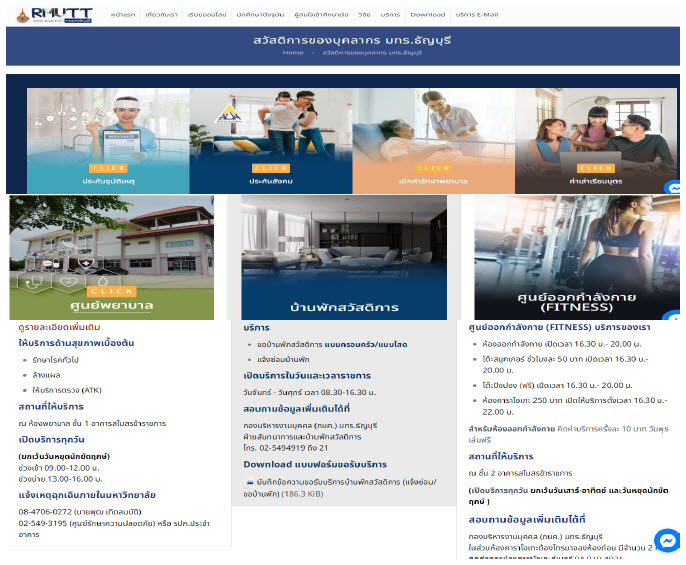
\includegraphics[width=0.9\textwidth]{Pic5.6-1.jpg}
	\caption{สวัสดิการของบุคลากร มทร.ธัญบุรี	ี}
	\label{Pic5.6-1}
\end{figure}
\end{center}

นอกจากนั้นในส่วนของมหาวิทยาลัยมีการจัดสวัสดิการที่เกี่ยวข้องกับการส่งเสริมสุขภาพที่ดี ประกอบด้วย
โครงการตรวจสุขภาพประจำปี สโมสร ศูนย์ออกกำลังกาย สระว่ายน้ำ สนามกีฬา การแข่งขันกีฬาบุคลากร และมีการสร้างขวัญและกำลังใจเพื่อให้บุคลากรทำงานได้อย่างมีประสิทธิภาพประสิทธิผล ประกอบด้วย การจัดทำประกันอุบัติเหตุให้กับบุคลากร เงินช่วยเหลือบุตร เงินช่วยเหลือค่าทำศพ บ้านพักสวัสดิการบุคลากร รางวัลบุคลากรดีเด่น การให้บุคลากรไปฝึกอบรมพัฒนาศึกษาดูงานทั้งในประเทศ/ต่างประเทศ นอกจากนี้คณะฯ ยังมีการจัดสวัสดิการและสิ่งจูงใจเพิ่มเติมนอกเหนือจากที่มหาวิทยาลัยจัดให้ดังนี้    
\begin{itemize}   
\item มีการประกาศยกย่องผู้ที่ได้ทำชื่อเสียงให้แก่คณะผ่านทางเว็บไซต์ของคณะฯ  
\item มีการจัดห้องออกกำลังกายให้กับบุคลากร 
\item มีการมอบของขวัญให้กับบุคลากรในวันขึ้นปีใหม่  
\item มีการปรับปรุงภูมิทัศน์ เพื่อส่งเสริมบรรยากาศที่ดีในการทำงาน
ในส่วนของสาขาวิชาคณิตศาสตร์ประยุกต์มีการสร้างแรงจูงใจและสวัสดิการให้แก่บุคลากรในสาขาวิชา ดังนี้
\item มีการประกาศยกย่องผู้ที่ได้ทำชื่อเสียงให้แก่สาขาวิชา ผ่านทางเว็บไซต์ของสาขาวิชา
\item มีการจัดหาสิ่งอำนวยความสะดวกในการดำรงชีพ เช่น ตู้เย็น ไมโครเวฟ เครื่องทำน้ำเย็น เครื่องทำ     น้ำร้อน น้ำดื่ม เครื่องชงกาแฟ ฯลฯ บริการแก่บุคลากรในสาขาวิชา
\item มีการจัดหาสิ่งอำนวยความสะดวกในการปฏิบัติงาน เช่น คอมพิวเตอร์ WIFI เครื่องพิมพ์ เครื่องถ่ายเอกสาร ฯลฯ บริการแก่บุคลากรในสาขาวิชานอกเหนือจากที่คณะจัดสรรให้
\item สาขาวิชามีการจัดเตรียมหนังสือ ตำรา ที่เกี่ยวข้องกับวิชาการ วิชาชีพ เพื่อบริการแก่บุคลากรในสาขาวิชา
\end{itemize}

ในส่วนของบทบาทหน้าที่ ความรับผิดชอบของอาจารย์ รวมทั้งจรรยาบรรณบุคลากร คณะและมหาวิทยาลัยมีการกำหนดแนวปฏิบัติต่างๆ รวมทั้งใช้แนวปฏิบัติของ สป.อว. เป็นกรอบดำเนินการ โดยมีการสื่อสารผ่านหัวหน้าสาขาวิชา มีการอบรมอาจารย์ใหม่ และมีข้อมูลรายละเอียดในเว็บไซต์ https://sci1.rmutt.ac.th/?page\_id=10368  เพื่อให้บุคลากรได้รับทราบตามแนวปฏิบัติ

\begin{figure}[h!]
	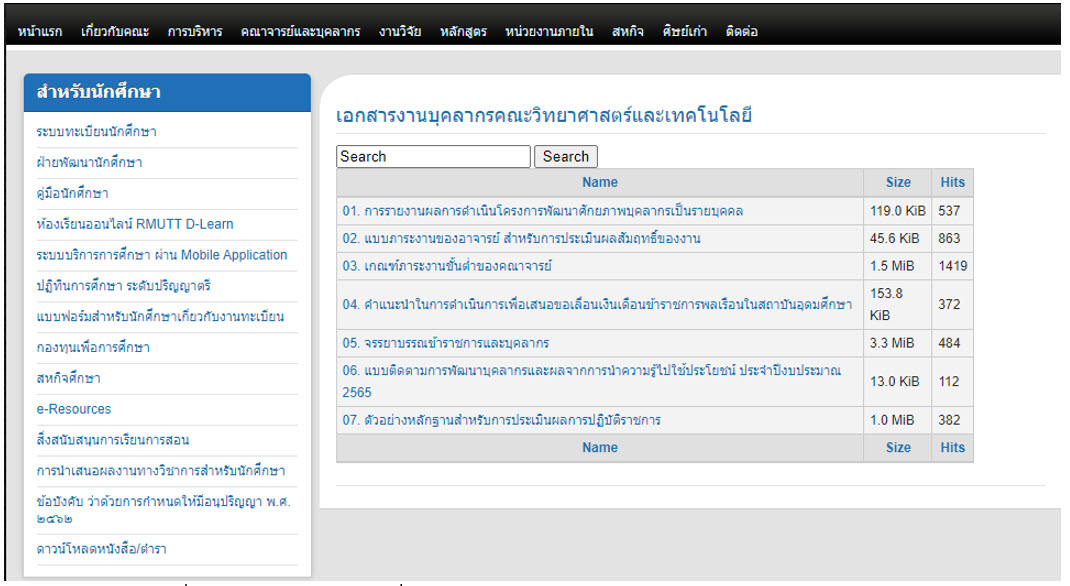
\includegraphics[width=\textwidth]{Pic5.6-2.jpg}
	\caption{บทบาทหน้าที่ความรับผิดชอบของอาจารย์และจรรยาบรรณบุคลากร}
	\label{Pic5.6-2}
\end{figure}
ในส่วนของความเป็นอิสระทางวิชาการ คณะและมหาวิทยาลัยได้ใช้แนวทางของ สป.อว. ตามประกาศเรื่องแนวปฏิบัติตามหลักความรับผิดชอบต่อสังคม หลักเสรีภาพทางวิชาการ หลักความเป็นอิสระ และหลักความเสมอภาค โดยทางหลักสูตร ได้แจ้งให้คณาจารย์ของหลักสูตรได้รับทราบผ่านการประชุมของหลักสูตร/อาจารย์ประจำสาขาวิชา
\begin{doclist}
	\docitem{เว็บไซต์คณะ : บทบาทหน้าที่ ความรับผิดชอบของอาจารย์ รวมทั้งจรรยาบรรณบุคลากร https://sci1.rmutt.ac.th/?page\_id=10368}
	\docitem{ราชกิจจานุเบกษา แนวปฏิบัติตามหลักความรับผิดชอบต่อสังคม หลักเสรีภาพทางวิชาการหลักความเป็นอิสระ และหลักความเสมอภาค}
\end{doclist}

%%%%%%%%%% 5.7 %%%%%%%%%%%%%%%
\subcriteria{The program to show that the training and developmental needs of the academic staff are systematically identified, and that appropriate training and development activities are implemented to fulfil the identified needs.}
นโยบายการพัฒนาบุคลากรด้านการฝึกอบรมของคณะฯ มุ่งเน้นไปที่ในแต่ละปีบุคลากรจะต้องพัฒนาตนเองตามสาขาวิชาชีพ และการพัฒนาตนเองตามยุทธศาสตร์ซึ่งจัดในภาพรวมที่จัดโดยคณะและมหาวิทยาลัย ในส่วนของคณะมีงบประมาณ 1,500 บาท/คน สำหรับให้บุคลากรพัฒนาตนเองตามวิชาชีพ ในส่วนของมหาวิทยาลัยมีงบประมาณจากงบพัฒนาบุคลากร 5,000 บาท/คนสำหรับจัดในภาพรวม ในแต่ละปีการศึกษามีกระบวนการในการดำเนินการพัฒนาบุคลากรด้านการฝึกอบรม  ดังนี้

\begin{figure}[h!]
	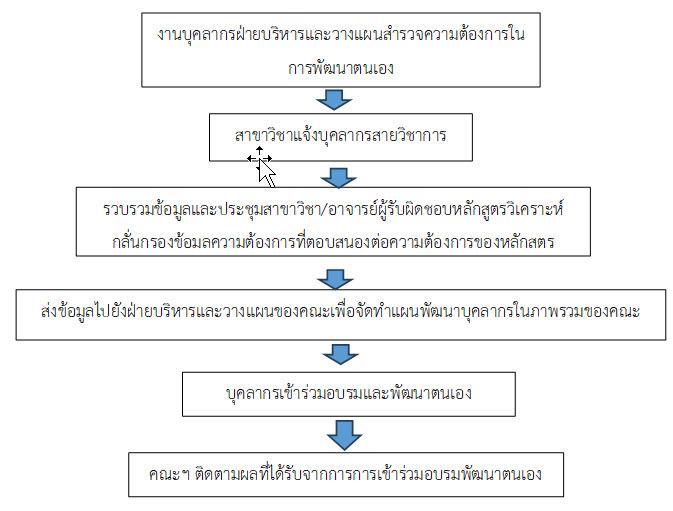
\includegraphics[width=\textwidth]{Pic5.7-1.jpg}
	\caption{กระบวนการพัฒนาบุคลากรด้านการฝึกอบรมพัฒนาตนเองของคณะ}
	\label{Pic5.7-1}
\end{figure}
หลักสูตรมีการประชุมจัดทำแผนการฝึกอบรม/พัฒนาบุคลากรสายวิชาการ เพื่อให้สอดคล้องกับความต้องการของหลักสูตร โดยให้อาจารย์ทุกท่านเข้ารับการฝึกอบรมทางด้านวิชาการ/วิชาชีพทางด้านคณิตศาสตร์หรือคณิตศาสตร์ประยุกต์อย่างน้อยปีละ 1 ครั้ง พร้อมทั้งรายงานผลการฝึกอบรมและการนำไปใช้ให้หลักสูตรทราบ

ในปีการศึกษา 2566 เนื่องจากหลักสูตรจะมีการประเมินคุณภาพหลักสูตรตามเกณฑ์มาตรฐาน AUN-QA จึงเพิ่มข้อกำหนดให้อาจารย์ทุกท่านเข้ารับการอบรม/พัฒนาตนเองด้านการประกันคุณภาพหลักสูตรตามเกณฑ์มาตรฐาน AUN-QA และจัดทำเป็นแผนให้อาจารย์ทุกท่านพัฒนาตนเอง ดังนี้
\begin{enumerate}
	\item ด้านวิชาการ/วิชาชีพทางด้านคณิตศาสตร์หรือคณิตศาสตร์ประยุกต์อย่างน้อยปีละ 1 ครั้ง
	\item ด้านการประกันคุณภาพหลักสูตรตามเกณฑ์มาตรฐาน AUN-QA อย่างน้อย 1 ครั้ง
\end{enumerate}

ผลการดำเนินงานในปีการศึกษา 2566 อาจารย์ทุกท่านเข้ารับการอบรม/พัฒนาตนเอง ตามแผนที่กำหนด รายละเอียดดังตาราง \ref{table: Teacher-Develop}

\begin{longtable}{|p{0.3\textwidth}|>{\raggedright}p{0.3\textwidth}|>{\raggedright}p{0.15\textwidth}|p{0.2\textwidth}|}
	\caption{การพัฒนาตนเองของบุคลาการสายวิชาการ สาขาวิชาคณิตศาสตร์}
	\label{table: Teacher-Develop}
	\\
	\hline
\textbf{ชื่อ-สกุล}&\textbf{หัวข้อที่เข้าอบรม}&\textbf{วันที่}
&\textbf{หน่วยงานที่จัด}\\\hline
	\endfirsthead
	\caption[]{(ต่อ) การพัฒนาตนเองของบุคลาการสายวิชาการ สาขาวิชาคณิตศาสตร์}
	\\
	\hline
\textbf{ชื่อ-สกุล}&\textbf{หัวข้อที่เข้าอบรม}&\textbf{วันที่}
&\textbf{หน่วยงานที่จัด}\\
	\hline
	\endhead

1. รศ.ดร.พงศกร สุนทรายุทธ์	&โครงการพัฒนาศักยภาพการปฏิบัติงานด้วยกระบวนการเชิงรุกสู่ความเป็นเลิศด้านคุณภาพการศึกษาและสร้างนวัตกรรมของ\newline บุคคลากรสายวิชาการ
&23-25 มิถุนายน 2566	
&คณะวิทยาศาสตร์และเทคโนโลยี มทร.ธัญบุรี\\
\cline{2-4} 
&โครงการอบรมเชิงปฏิบัติการ การเขียนรายงานการประเมินตนเอง (SAR) ตามเกณฑ์ประกันคุณภาพการศึกษาอาเซียน (ASEAN University Network Quality Assurance : AUN-QA)	
&18-19 ธันวาคม 2566	
&คณะวิทยาศาสตร์และเทคโนโลยี มทร.ธัญบุรี\\
\hline
%%%====================================
2. ผศ.กุลประภา ศรีหมุด
&โครงการพัฒนาศักยภาพการปฏิบัติงานด้วยกระบวนการเชิงรุกสู่ความเป็นเลิศด้านคุณภาพการศึกษาและสร้างนวัตกรรมของ\newline บุคคลากรสายวิชาการ	&23-25 มิถุนายน 2566	
&คณะวิทยาศาสตร์และเทคโนโลยี มทร.ธัญบุรี\\
\cline{2-4}
&บรรยายพิเศษหัวข้อ “Python for industrial and application”	
&12 ตุลาคม 2566
&สาขาวิชาคณิตศาสตร์ คณะวิทยาศาสตร์และเทคโนโลยี มทร.ธัญบุรี\\             
\cline{2-4} 
%%%%%%%%%%%%%%%%%%%%%9-3

&โครงการอบรมเชิงปฏิบัติการ\newline การเขียนรายงานการประเมินตนเอง (SAR) ตามเกณฑ์ประกันคุณภาพการศึกษาอาเซียน (ASEAN University Network Quality Assurance : AUN-QA)
&18-19 ธันวาคม 2566	
&คณะวิทยาศาสตร์และเทคโนโลยี มทร.ธัญบุรี\\
\hline
%===================================
3. ผศ.สมนึก ศรีสวัสดิ์
&บรรยายพิเศษ เรื่อง Mathematics and statistics in Data Science
&26 กรกฎาคม 2566	
&คณะวิทยาศาสตร์และเทคโนโลยี มทร.ธัญบุรี\\
\cline{2-4}
&บรรยายพิเศษหัวข้อ “Python for industrial and application”	
&12 ตุลาคม 2566	
&สาขาวิชาคณิตศาสตร์ คณะวิทยาศาสตร์และเทคโนโลยี มทร.ธัญบุรี\\
\cline{2-4} 
&โครงการอบรมเชิงปฏิบัติการ\newline การเขียนรายงานการประเมินตนเอง (SAR) ตามเกณฑ์ประกันคุณภาพการศึกษาอาเซียน (ASEAN University Network Quality Assurance : AUN-QA)
&18 ธันวาคม 2566	
&คณะวิทยาศาสตร์และเทคโนโลยี มทร.ธัญบุรี\\ 
\hline
%============================================
4. ผศ.ดร.กมลรัตน์ สมบุตร&บรรยายพิเศษ เรื่อง Mathematics and statistics in Data Science
& 26 กรกฎาคม\newline 2566                  
&สาขาวิชาคณิตศาสตร์และสาขาวิชาสถิติ\newline คณะวิทยาศาสตร์และเทคโนโลยี มทร.ธัญบุรี\\
\cline{2-4} 
&บรรยายพิเศษหัวข้อ\newline “Python for industrial and application”	
&12 ตุลาคม 2566	
&สาขาวิชาคณิตศาสตร์ คณะวิทยาศาสตร์และเทคโนโลยี มทร.ธัญบุรี\\ 
\cline{2-4}
&โครงการอบรมเชิงปฏิบัติการ\newline การเขียนรายงานการประเมินตนเอง (SAR) ตามเกณฑ์ประกันคุณภาพการศึกษาอาเซียน (ASEAN University Network Quality Assurance : AUN-QA)
&18-19 ธันวาคม 2566	
&คณะวิทยาศาสตร์และเทคโนโลยี\\ 
\hline
%=========================================
5. ผศ.ดร.วงศ์วิศรุต เขื่องสตุ่ง
&บรรยายพิเศษ เรื่อง Mathematics and statistics in Data Science
&26 กรกฎาคม 2566	
&สาขาวิชาคณิตศาสตร์และสาขาวิชาสถิติ\newline คณะวิทยาศาสตร์และเทคโนโลยี มทร.ธัญบุรี\\
\cline{2-4} 
&Data Science Tools	
&14 ธันวาคม 2566	
&ระบบออนไลน์\\             
\cline{2-4} &Data Science Methodologies	
&10 มกราคม 2567	
&ระบบออนไลน์\\             
\hline
%===========================
6. ผศ.ดร.ภคีตา สุขประเสริฐ
&โครงการพัฒนาศักยภาพการปฏิบัติงานด้วยกระบวนการเชิงรุกสู่ความเป็นเลิศด้านคุณภาพการศึกษาและสร้างนวัตกรรมของ\newline บุคคลากรสายวิชาการ	&23-25 มิถุนายน 2566	
&คณะวิทยาศาสตร์และเทคโนโลยี มทร.ธัญบุรี\\             
\cline{2-4} &ฟังบรรยายพิเศษหัวข้อ “Mathematics and statistics in daily life”	
&26 มิถุนายน 2566	
&สาขาวิชาคณิตศาสตร์และสาขาวิชาสถิติ\newline คณะวิทยาศาสตร์และเทคโนโลยี มทร.ธัญบุรี\\
\cline{2-4}
 &บรรยายพิเศษหัวข้อ “Python for industrial and application”	
&12 ตุลาคม 2566	
&สาขาวิชาคณิตศาสตร์ คณะวิทยาศาสตร์และเทคโนโลยี มทร.ธัญบุรี\\             
\hline
 &โครงการอบรมเชิงปฏิบัติการ\newline การเขียนรายงานการประเมินตนเอง (SAR) ตามเกณฑ์ประกันคุณภาพการศึกษาอาเซียน (ASEAN University Network Quality Assurance : AUN-QA)
&18 ธันวาคม 2566	
&คณะวิทยาศาสตร์และเทคโนโลยี มทร.ธัญบุรี\\ 
\hline 
%================================
7. ผศ.ดร.ปริญญวัฒน์ 
ชูสุวรรณ	
&บรรยายพิเศษหัวข้อเรื่อง Beyond the Banach Contraction Principle& 15 มิถุนายน 2566 &ภาควิชาคณิตศาสตร์และวิทยาการคอมพิวเตอร์ คณะวิทยาศาสตร์ จุฬาลงกรณ์มหาวิทยาลัย\\
\cline{2-4}
&โครงการอบรมเชิงปฏิบัติการ\newline การเขียนรายงานการประเมินตนเอง (SAR) ตามเกณฑ์ประกันคุณภาพการศึกษาอาเซียน (ASEAN University Network Quality Assurance : AUN-QA)
&18-19 ธันวาคม 2566	
&คณะวิทยาศาสตร์และเทคโนโลยี\\
\hline
%=============================
8. ผศ.มงคล ทาทอง
&โครงการอบรมเชิงปฏิบัติการ เรื่อง AUN-QA Implementation and Gap Analysis รุ่นที่ 1	
&29-30 พฤศจิกายน 2566
&คณะวิทยาศาสตร์และเทคโนโลยี\\ 
\cline{2-4}
&โครงการอบรมเชิงปฏิบัติการ\newline การเขียนรายงานการประเมินตนเอง (SAR) ตามเกณฑ์ประกันคุณภาพการศึกษาอาเซียน (ASEAN University Network Quality Assurance : AUN-QA)
&18-19 ธันวาคม 2566
&คณะวิทยาศาสตร์และเทคโนโลยี\\
\hline
%==================================
9. ดร.นนธิยา มากะเต&บรรยายพิเศษ เรื่อง Mathematics and statistics in Data Science
& 26 กรกฎาคม\newline 2566                  
&สาขาวิชาคณิตศาสตร์และสาขาวิชาสถิติ\newline คณะวิทยาศาสตร์และเทคโนโลยี มทร.ธัญบุรี\\
\cline{2-4} 
&บรรยายพิเศษหัวข้อ\newline “Python for industrial and application”	
&12 ตุลาคม 2566	
&สาขาวิชาคณิตศาสตร์ คณะวิทยาศาสตร์และเทคโนโลยี มทร.ธัญบุรี\\ 
\hline
&โครงการอบรมเชิงปฏิบัติการ\newline การเขียนรายงานการประเมินตนเอง (SAR) ตามเกณฑ์ประกันคุณภาพการศึกษาอาเซียน (ASEAN University Network Quality Assurance : AUN-QA)
&18-19 ธันวาคม 2566	
&คณะวิทยาศาสตร์และเทคโนโลยี\\ 
\hline
%=========================================
10. ดร.วรรณา ศรีปราชญ์
&บรรยายพิเศษหัวข้อ “Python for industrial and application”	
&12 ตุลาคม 2566	
&สาขาวิชาคณิตศาสตร์ คณะวิทยาศาสตร์และเทคโนโลยี มทร.ธัญบุรี\\ 
\cline{2-4}
&โครงการอบรมเชิงปฏิบัติการ\newline การเขียนรายงานการประเมินตนเอง (SAR) ตามเกณฑ์ประกันคุณภาพการศึกษาอาเซียน (ASEAN University Network Quality Assurance : AUN-QA)
&18-19 ธันวาคม 2566	
&คณะวิทยาศาสตร์และเทคโนโลยี มทร.ธัญบุรี\\
\hline
%===============================
11. ดร.รัฐพรหม พรหมคำ	&บรรยายพิเศษหัวข้อ “Python for industrial and application”	
&12 ตุลาคม 2566	
&สาขาวิชาคณิตศาสตร์ คณะวิทยาศาสตร์และเทคโนโลยี มทร.ธัญบุรี\\ 
\cline{2-4}
&โครงการอบรมเชิงปฏิบัติการ\newline การเขียนรายงานการประเมินตนเอง (SAR) ตามเกณฑ์ประกันคุณภาพการศึกษาอาเซียน (ASEAN University Network Quality Assurance : AUN-QA)
&18-19 ธันวาคม 2566	
&คณะวิทยาศาสตร์และเทคโนโลยี มทร.ธัญบุรี\\
\hline
%===============================
12. อ.อลงกต สุวรรณมณี
&บรรยายพิเศษ เรื่อง Mathematics and statistics in Data Science
& 26 กรกฎาคม\newline 2566                  
&สาขาวิชาคณิตศาสตร์และสาขาวิชาสถิติ\newline คณะวิทยาศาสตร์และเทคโนโลยี มทร.ธัญบุรี\\
\cline{2-4} 
&โครงการอบรมเชิงปฏิบัติการ\newline การเขียนรายงานการประเมินตนเอง (SAR) ตามเกณฑ์ประกันคุณภาพการศึกษาอาเซียน (ASEAN University Network Quality Assurance : AUN-QA)
&18-19 ธันวาคม 2566	
&คณะวิทยาศาสตร์และเทคโนโลยี มทร.ธัญบุรี\\
\hline
%===================================
13. อ.โอม สถิตยนาค
&บรรยายพิเศษ เรื่อง Mathematics and statistics in Data Science
& 26 กรกฎาคม\newline 2566                  
&สาขาวิชาคณิตศาสตร์และสาขาวิชาสถิติ\newline คณะวิทยาศาสตร์และเทคโนโลยี มทร.ธัญบุรี\\
\cline{2-4} 
&บรรยายพิเศษหัวข้อ\newline “Python for industrial and application”	
&12 ตุลาคม 2566	
&สาขาวิชาคณิตศาสตร์ คณะวิทยาศาสตร์และเทคโนโลยี มทร.ธัญบุรี\\ 
\cline{2-4}
&โครงการอบรมเชิงปฏิบัติการ\newline การเขียนรายงานการประเมินตนเอง (SAR) ตามเกณฑ์ประกันคุณภาพการศึกษาอาเซียน (ASEAN University Network Quality Assurance : AUN-QA)
&18-19 ธันวาคม 2566	
&คณะวิทยาศาสตร์และเทคโนโลยี\\ 
\hline
%=========================================
14. อ.วาสนา ทองกำแหง	&บรรยายพิเศษ เรื่อง Mathematics and statistics in Data Science
& 26 กรกฎาคม\newline 2566                  
&สาขาวิชาคณิตศาสตร์และสาขาวิชาสถิติ\newline คณะวิทยาศาสตร์และเทคโนโลยี มทร.ธัญบุรี\\
\cline{2-4} 
&บรรยายพิเศษหัวข้อ\newline “Python for industrial and application”	
&12 ตุลาคม 2566	
&สาขาวิชาคณิตศาสตร์ คณะวิทยาศาสตร์และเทคโนโลยี มทร.ธัญบุรี\\ 
\cline{2-4}
&โครงการอบรมเชิงปฏิบัติการ\newline การเขียนรายงานการประเมินตนเอง (SAR) ตามเกณฑ์ประกันคุณภาพการศึกษาอาเซียน (ASEAN University Network Quality Assurance : AUN-QA)
&18-19 ธันวาคม 2566	
&คณะวิทยาศาสตร์และเทคโนโลยี\\ 
\hline
%=====================================
15. อ.อัคเรศ สิงห์ทา&\multicolumn{3}{c|}{ลาศึกษาต่อ}\\
\hline
%====================================
16. อ.อมราภรณ์ บำเพ็ญดี
&บรรยายพิเศษ เรื่อง Mathematics and statistics in Data Science	
&26 กรกฎาคม 2566	
&คณะวิทยาศาสตร์และเทคโนโลยี มทร.ธัญบุรี\\             
\cline{2-4}
&บรรยายพิเศษหัวข้อ “Python for industrial and application”	
&12 ตุลาคม 2566	
&สาขาวิชาคณิตศาสตร์ คณะวิทยาศาสตร์และเทคโนโลยี มทร.ธัญบุรี\\             
\hline
&โครงการอบรมเชิงปฏิบัติการ\newline การเขียนรายงานการประเมินตนเอง (SAR) ตามเกณฑ์ประกันคุณภาพการศึกษาอาเซียน (ASEAN University Network Quality Assurance : AUN-QA)
&18 ธันวาคม 2566	
&คณะวิทยาศาสตร์และเทคโนโลยี มทร.ธัญบุรี\\ 
\hline
%=======================================
17. อ.ธาวัลย์ อัมพวา
&บรรยายพิเศษ เรื่อง Mathematics and statistics in Data Science	
&26 กรกฎาคม 2566	
&คณะวิทยาศาสตร์และเทคโนโลยี มทร.ธัญบุรี\\             
\cline{2-4} 
&โครงการอบรมเชิงปฏิบัติการ\newline การเขียนรายงานการประเมินตนเอง (SAR) ตามเกณฑ์ประกันคุณภาพการศึกษาอาเซียน (ASEAN University Network Quality Assurance : AUN-QA)
&18-19 ธันวาคม 2566
&คณะวิทยาศาสตร์และเทคโนโลยี\\             
\hline
%=========================================
18. ดร.ปฤณท์ธพร สงวนสุทธิกุล
&โครงการอบรมเชิงปฏิบัติการการออกแบบการเรียนรู้เชิงรุกด้วยกรอบแนวคิดซีดีไอโอ (Design a CDIO-based Active Learning Experiences)	
&23-24 มิถุนายน 2566	
&คณะวิศวกรรมศาสตร์ มทร.ธัญบุรี\\
\cline{2-4} 
&The 11th Asian Conference on Fixed Point Theory and Optimization 2023	
&4-5 สิงหาคม 2566	
&A-one royal cruise\newline hotel, Pattaya,\newline Thailand\\             
\cline{2-4} 
&เข้าร่วมงานสัมมนา TaCS Seminar Series No.13-14	
&11 ธันวาคม  2566	
&ภาควิชาคณิตศาสตร์ คณะวิทยาศาสตร์ มหาวิทยาลัยเทคโนโลยีพระจอมเกล้าธนบุรี\\  
\hline    
\end{longtable}

\begin{doclist}
	\docitem{แผนพัฒนาตนเองรายบุคคล (IDP) ปีการศึกษา 2566}
\end{doclist}

%%%%%%%%%% 5.8 %%%%%%%%%%%%%%%
\subcriteria{The program to show that performance management including reward and recognition is implemented to assess academic staff teaching and research quality.}

หลักสูตรวิทยาศาสตรบัณฑิต สาขาวิชาคณิตศาสตร์ประยุกต์ ใช้แนวทางการประเมินผลการปฏิบัติงานของอาจารย์ตามระบบจัดการข้อมูลการประเมินบุคลากรคณะวิทยาศาสตร์และเทคโนโลยีโดยจะประเมิน 2 ครั้ง ครั้งที่ 1 คือ 1 ตุลาคม ถึง 31 มีนาคม และ
ครั้งที่ 2 คือ 1 เมษายน ถึง 30 กันยายน
 โดยคะแนนประเมินจะมาจาก 2 ส่วนประกอบคือ 
\begin{enumerate}
\item ภาระงานด้านการเรียนการสอน วิจัย การบริการทางวิชาการ งานมอบหมายอื่น ๆ และการหารายได้ คิดเป็นสัดส่วนคะแนน 70\%
\item ประเมินสมรรถนะหลักของบุคลากรสายวิชาการที่กำหนดโดยมหาวิทยาลัย 6 ด้าน คิดเป็นสัดส่วนคะแนน 30\%
\end{enumerate}

เมื่อบุคลากรสายวิชาการเนินการประเมินผลงานเรียบร้อยแล้ว  จะมีการแจ้งผลการประเมินเพื่อสะท้อนให้เห็นผลการปฏิบัติงาน และผู้ถูกประเมินรับทราบผลการประเมินเพื่อนำผลการประเมินนำไปปรับปรุงในรอบถัดไป หลังจากนั้นคณะนำเสนอข้อมูลไปยังมหาวิทยาลัย เพื่อพิจารณาอนุมัติการขึ้นเงินเดือน และจะมีการแจ้งผลการขึ้นเงินเดือนของแต่ละรายบุคคลผ่านเว็บไซต์ www.hr.rmutt.ac.th โดยบุคลากรสายวิชาการแต่ละคนต้อง log in ด้วย username และ password ของตนเอง

มีการสร้างขวัญกำลังใจ การยกย่องเชิดชูเกียรติ การให้รางวัล ทั้งของระดับหลักสูตรฯ ระดับคณะฯ และระดับมหาวิทยาลัย 

ในส่วนของระดับคณะฯ และหลักสูตรฯ มีการแสดงยินดีผ่าน Web-site/Facebook ของคณะฯ และสาขาวิชาฯ ซึ่ง
ในปีการศึกษา 2566 มีบุคลากรสายวิชาการของสาขาวิชาที่ได้รับการตีพิมพ์บทความทางวิชาการ ในฐานข้อมูล Scopus Q1 จำนวน 2 ท่าน คือ ผศ.ดร.วงศ์วิศรุต เขื่องสตุ่ง และ ผศ.ดร.กมลรัตน์ สมบุตร และได้มีการแสดงความยินดีผ่าน website และ Facebook ดังภาพที่ \ref{Pic5.8-1}
\begin{figure}[h!]
	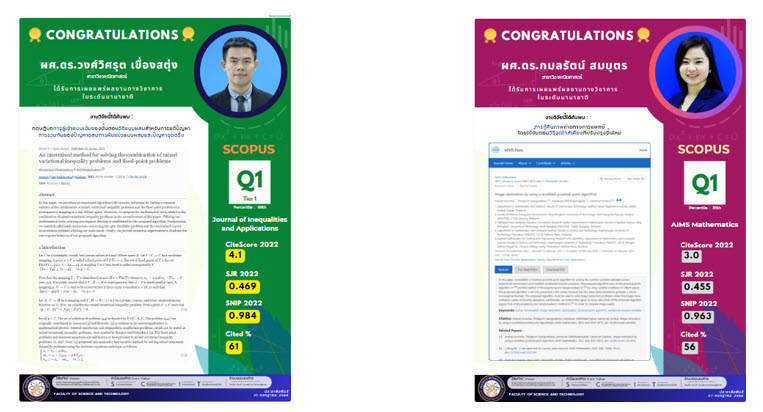
\includegraphics[width=\textwidth]{Pic5.8-1.jpg}
	\caption{บุคลากรของสาขาวิชาที่ได้รับการตีพิมพ์บทความทางวิชาการ ในฐานข้อมูล Scopus Q1}
	\label{Pic5.8-1}
\end{figure}

นอกจากนี้ในระดับมหาวิทยาลัยยังมีการให้เงินรางวัล ทางด้านรางวัลสำหรับอาจารย์ที่มีผลงานวิจัยเผยแพร่รายละเอียดดังตารางที่ \ref{Table:award}
\begin{center}
		\begin{longtable}{|p{0.55\textwidth}|p{0.4\textwidth}|}
			 \caption{อัตราเงินรางวัลสำหรับอาจารย์ที่เผยแพร่ผลงานทางวิชาการ}
			\label{Table:award}\\
			\hline
		   \textbf{รูปแบบการเผยแพร่ผลงานทางวิชาการ}	&\textbf{เงินรางวัล/ผลงาน (บาท)}\\
		  	 \hline
			\endhead
			%%%%%%%%%%%%%%%%%%%%%%%%%%
			\multicolumn{2}{|l|}{\textbf{วารสารวิชาการระดับชาติ}	
		}\\
			\hline
			ค่าสมนาคุณการตีพิมพ์บทความวิจัยในวารสารระดับชาติที่อยู่ในฐานข้อมูล TCI กลุ่ม 1 หรือ กลุ่ม 2	&4,000 บาท\\
			\hline
			ค่าธรรมเนียมการตีพิมพ์บทความวิจัย (Page   charge) ของวารสารที่อยู่ในฐานข้อมูล TCI      	&ตามที่จ่ายจริงแต่ไม่เกิน  5,000 บาท\\
			\hline
			\multicolumn{2}{|l|}{\textbf{วารสารวิชาการระดับนานาชาติ}}\\
			\hline
			ค่าสมนาคุณการตีพิมพ์บทความวิจัย Scopus Top 10% หรือ Tier 1
			&60,000 บาท\\
			\hline
			ค่าสมนาคุณการตีพิมพ์บทความวิจัยควอไทล์ที่ 1 (Q1)         	&30,000 บาท	\\
			\hline
			ค่าสมนาคุณการตีพิมพ์บทความวิจัย ควอไทล์ที่ 2 (Q2)         	&20,000 บาท	\\
			\hline
			ค่าสมนาคุณการตีพิมพ์บทความวิจัย ควอไทล์ที่ 3 (Q3)         	&10,000 บาท\\
			\hline
			ค่าสมนาคุณการตีพิมพ์บทความวิจัย ควอไทล์ที่ 4 (Q4)         	&8,000 บาท	\\
			\hline
			ไม่มีควอไทล์ 	&4,000 บาท	\\
			\hline
			ค่าธรรมเนียมการตีพิมพ์บทความวิจัย (Page Charge) ที่อยู่ในกลุ่มอันดับ TOP 10 \% หรือ Tier 1 ให้สนับสนุนตามที่จ่ายจริงหลังหักค่าสมนาคุณการตีพิมพ์บทความวิจัยแล้ว  &\\
			\hline
			\multicolumn{2}{|l|}{\textbf{กรณีตีพิมพ์ในวารสาร ประเภทบทความวิจัยที่ถูกคัดเลือกมาจากการประชุมวิชาการ}}\\[-0.15cm]
				\multicolumn{2}{|l|}{\textbf{และนำมาตีพิมพ์ลงในวารสาร (Journal) และเป็นฉบับพิเศษ (Special Issue)}}\\
			\hline
			ค่าสมนาคุณการตีพิมพ์บทความวิจัย Scopus Top 10\% หรือ Tier 1	&15,000 บาท\\
			\hline
			ค่าสมนาคุณการตีพิมพ์บทความวิจัยควอไทล์ที่ 1 (Q1)         	&7,500 บาท\\
			\hline
			ค่าสมนาคุณการตีพิมพ์บทความวิจัย ควอไทล์ที่ 2 (Q2)         	&5,000 บาท\\
			\hline
			ค่าสมนาคุณการตีพิมพ์บทความวิจัย ควอไทล์ที่ 3 (Q3)         	&2,500 บาท\\
			\hline
			ค่าสมนาคุณการตีพิมพ์บทความวิจัย ควอไทล์ที่ 4 (Q4)         	&2,000 บาท\\
			\hline
			ไม่มีควอไทล์	&1,000 บาท\\
			\hline
			\multicolumn{2}{|l|}{\textbf{ค่าสมนาคุณงานสร้างสรรค์ที่เผยแพร่}}\\
			\hline
			งานสร้างสรรค์ที่เผยแพร่ในระดับภูมิภาคอาเซียน/นานาชาติ     	&8,000 บาท\\
			\hline
			งานสร้างสรรค์ที่เผยแพร่ในระดับความร่วมมือระหว่างประเทศ  	&4,000 บาท\\
			\hline
			งานสร้างสรรค์ที่เผยแพร่ในระดับชาติ                                	&3,000 บาท\\
			\hline
			งานสร้างสรรค์ที่เผยแพร่ในระดับสถาบัน                            	&1,500 บาท\\
			\hline
	\end{longtable}
\end{center}
\begin{doclist}
	\docitem{แนวทางการประเมินผลการปฏิบัติงานบุคลากรสายวิชาการ คณะวิทยาศาสตร์และเทคโนโลยี}
	\docitem{เกณฑ์รางวัลสมนาคุณการตีพิมพ์บทความวิจัย}
	\docitem{ภาพแสดงความชื่นชมยินดี ผ่านเว็บไซต์คณะ Facebook ของสาขาวิชา}
\end{doclist}
\newpage
\criteria{Student Support Services}

\subcriteria{ The student intake policy, admission criteria, and admission procedures to the programme are shown to be clearly defined, communicated, published, and up-to-date.}
\noindent
{\bf การรับนักศึกษา}

	หลักสูตรกำหนดแผนการรับนักศึกษาปีละ 30 คน โดยรกำหนดนโยบายการรับนักศึกษา ช่องทางการรับเข้า คุณสมบัติของนักศึกษาที่จะรับเข้าศึกษา รวมถึงวิธีการคัดเลือกนักศึกษา และได้สื่อสารเผยแพร่ไปยังผู้มีส่วนได้ส่วนเสีย ได้แก่ นักเรียนชั้นมัธยมศึกษาปีที่ 6 ผู้ปกครอง และผู้ที่สนใจทั่วไป ผ่านเว็บไซต์ของมหาวิทยาลัยฯ คณะฯ และของสาขาวิชา รวมทั้ง Facebook ของคณะและสาขาวิชาฯ นอกจากนี้มีการออกประชาสัมพันธ์แนะแนวตามโรงเรียนที่เป็นกลุ่มเป้าหมายและโรงเรียนที่มีความร่วมมือทางวิชาการ (MOU)   กรอบการดำเนินงานเกี่ยวกับการรับนักศึกษาเป็นไปตามที่สำนักส่งเสริมวิชาการและงานทะเบียน (สวท.) เป็นผู้กำหนด เช่น ปฏิทินการรับสมัคร ระบบการสมัครทางระบบออนไลน์ การประกาศผล ฯลฯ ทั้งนี้ในแต่ละปีการศึกษากระบวนการรับนักศึกษามีขั้นตอนการดำเนินการดังนี้
	\begin{enumerate}
		\item งานทะเบียนฝ่ายวิชาการแจ้งให้หลักสูตรจัดทำข้อมูลรายละเอียดการรับสมัครนักศึกษาใหม่ เช่น จำนวนรับ คุณสมบัติผู้สมัคร วิธีการสอบคัดเลือก และคำแนะนำเกี่ยวกับหลักสูตร
		\item หลักสูตรจัดเตรียมข้อมูลเกณฑ์การรับ คุณสมบัติของนักศึกษา และแผนการรับนักศึกษา และส่งให้งานทะเบียนของคณะ 
		\item งานทะเบียนของคณะส่งข้อมูลเกณฑ์การรับ/คุณสมบัติของนักศึกษา แผนรับนักศึกษาไปยัง สวท. ของมหาวิทยาลัย เพื่อนำเข้าสู่การประชุมคณะกรรมการการบริหารวิชาการและวิจัย เพื่อพิจารณาอนุมัติและกำหนดไว้ในคู่มือการรับนักศึกษา
	\end{enumerate}
เมื่อได้รับกสนอนุมัติแผนรับแล้วหลักสูตรดำเนินการตามขั้นตอน วัน-เวลา การดำเนินการของมหาวิทยาลัยต่อไป\\

%%%%%%%%%%%%%%%%%%%%%%
\noindent{\bf เกณฑ์และขั้นตอนการรับเข้า}\\[0.5cm]
หลักสูตรกำหนดเกณฑ์การรับเข้าตามรอบการรับสมัครทั้งหมด 5 รอบ ได้แก่
	\begin{enumerate}
		\item โควตา MOU
		\item TCAS 1
		\item TCAS 2
		\item TCAS 3
		\item TCAS 4
	\end{enumerate}
โดยเกณฑ์และคุณสมบัติของนักศึกษาที่จะรับเข้าในแต่ละรอบมีรายละเอียด\underline{ดังเอกสารหลักฐานระเบียบการรับสมัคร}
และแต่ละรอบมีขั้นตอนและกำหนดการสมัครดังรูป
\ref{Pic6.1-01}\\
\begin{figure}[h!]
	\begin{center}
		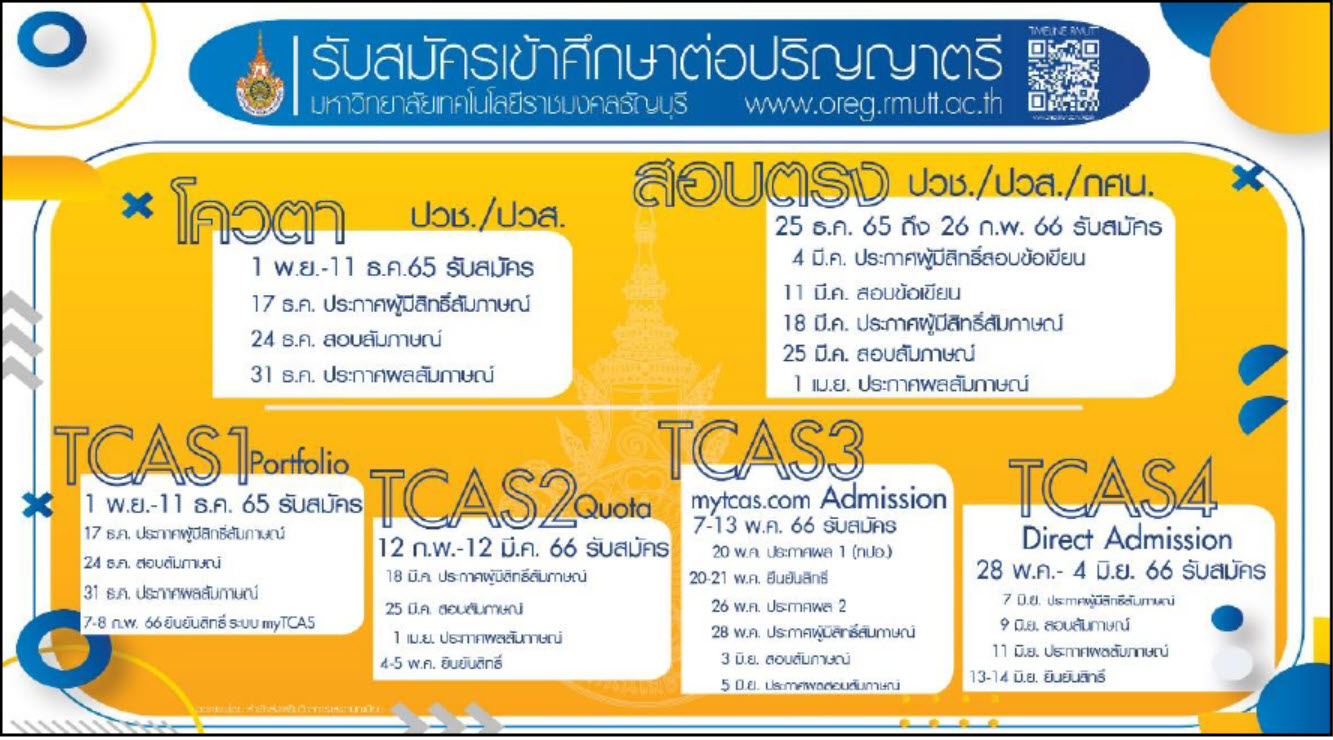
\includegraphics[width=0.9\textwidth]{Pic6.1-01.jpg}
		\end{center}
	\caption{รอบการรับสมัครและช่วงเวลาการรับสมัคร}
	\label{Pic6.1-01}
\end{figure}\\
ผลการดำเนินงานเกี่ยวกับการรับนักศึกษาในปีการศึกษา 2564-2566 หลักสูตรวิทยาศาสตรบัณฑิต สาขาวิชาคณิตศาสตร์ แสดงได้ดังตาราง \ref{table:6.1}
\newpage
\begin{longtable}{ |c|c|c|c|c|c|c|  }
\caption{ข้อมูลเปรียบเทียบแผนรับและจำนวนนักศึกษาที่รายงานตัวปีการศึกษา 2564-2566 }
\label{table:6.1}\\
 \hline
 \multicolumn{7}{|c|}{แผนรับ/รายงานตัว ปีการศึกษา 2564 – 2566} \\
 \hline
  & \multicolumn{2}{c|}{2564} & \multicolumn{2}{c|}{2565} & \multicolumn{2}{c|}{2566} \\
 \hline
 ช่องทางการรับเข้า & แผนรับ & รายงานตัว & แผนรับ & รายงานตัว & แผนรับ & รายงานตัว \\
 \hline
  TCAS 1 & 10 & 6 & 15 & 5 &  15 &   1 \\
 \hline
   TCAS 2& 10 & 3 & 8 & 2 &  7 &   0 \\
 \hline
   TCAS 3& 4 & 5 & 6 & 5 &  7 &  7  \\
 \hline
   TCAS 4 & 2 & 2 & 1 & 2 & 1  & 2   \\
 \hline
 โควตา MOU  & 4 & 18 & - &  9 & -  & 1   \\
 \hline
  รวม  & 30 & 34 & 30 &  23 & 30  &  11  \\
 \hline
\end{longtable}

จากตารางพบว่าแนวโน้มยอดนักศึกษารับเข้าลดลงอย่างต่อเนื่องซึ่งทางหลักสูตรจะดำเนินการปรับปรุงกระบวนการรับเข้าต่อไป
     
  นอกจากนี้หลักสูตรได้สำรวจเกี่ยวกับช่องทางการประชาสัมพันธ์ของนักศึกษาที่รับเข้าในปีการศึกษา 2566 มีผลดังตาราง \ref{table:6.2}
  \newpage
\begin{longtable}{ |>{\raggedright}p{6cm}|c|}
\caption{การรับรู้จากสื่อการประชาสัมพันธ์ของนักศึกษาที่รับเข้าในปีการศึกษา 2566}
\label{table:6.2}\\
 
\hline
\multicolumn{1}{|c|}{{\bf ช่องทางการประชาสัมพันธ์}}     & \multicolumn{1}{c|}{\textbf{ร้อยละของผู้ตอบแบบสอบถาม }}                 \\ \hline
1. เพื่อน  &   11.54\\ 
\hline
2. ครูแนะแนว &   25 \\ 
\hline
3. แนะแนวสัญจร &   11.54 \\ 
\hline
4. เว็บไซค์คณะวิทยาศาสตร์และเทคโนโลยี มทร.ธัญบุรี &  38.46  \\ 
\hline
5. เพจคณะวิทยาศาสตร์และเทคโนโลยี มทร.ธัญบุรี   &   1.92 \\ 
\hline
6. เพจสาขาวิชาคณิตศาสตร์คณะวิทยาศาสตร์และเทคโนโลยี มทร.ธัญบุรี &  5.77  \\ 
\hline
7. อื่นๆ  & 5.77  \\ 
\hline
\end{longtable}

    
 
 \begin{doclist}
 	\docitem{เว็บไซต์/ Facebook การประชาสัมพันธ์}
 	\docitem{ระเบียบการรับสมัครนักศึกษาปีการศึกษา 2566}
 \end{doclist}

%%%%%%%%%%%%%% 6.2 %%%%%%%%%%%%%%%
\subcriteria{Both short-term and long-term planning of academic and non-academic support services are shown to be carried out to ensure sufficiency and quality of support services for teaching, research, and community service.}



หลักสูตรมีการบริการสนับสนุนทางด้านวิชาการและที่ไม่ใช่ทางวิชาการ เพื่อพัฒนาทักษะของนักศึกษาโดยมีการดำเนินการกิจกรรม ตามแผนงานที่จัดทำเพื่อพัฒนาประสบการณ์ ทางวิชาการและวิชาชีพแก่ นักศึกษาโดยมีกิจกรรม ดังนี้\\

\noindent
\textbf{แผนงานระยะสั้น}
\begin{longtable}{ |>{\raggedright}p{3cm}|p{10.5cm}|} 
\hline
\centering{\textbf{กิจกรรม}}   &\multicolumn{1}{c|}{\textbf{รายละเอียด}} \\ \hline
\endhead
1. กิจกรรมบรรยายพิเศษ ในหัวข้อ “Mathematics and statistics in Data Science” โดย Professor Yeol Je Cho   & สาขาวิชาคณิตศาสตร์ร่วมกับสาขาวิชาสถิติประยุกต์ คณะวิทยาศาสตร์และเทคโนโลยี จัดบรรยายพิเศษ ในหัวข้อ “Mathematics and statistics in Data Science” โดย Professor Yeol Je Cho วิทยากรจาก Department of Mathematics Education Gyeongsang National University Jin 52828, KOREA ในวันที่ 26 กรกฎาคม 2566 ณ ห้องประชุมนลินวิทย์ คณะวิทยาศาสตร์และเทคโนโลยี มหาวิทยาลัยเทคโนโลยีราชมงคลธัญบุรีเทคโนโลยี
โดยมีวัตถุประสงค์ ดังนี้ เพื่อให้นักศึกษามีความรู้และความเข้าใจเกี่ยวกับการใช้คณิตศาสตร์และสถิติในการประยุกต์ทางด้าน Data Science
\\ 
\hline
2. กิจกรรมบรรยายพิเศษ ในหัวข้อ "Python for industrial and application" โดยคุณจิรพัฒน์  ลิ้มธนะกุล Western Digital Storage Technologies\newline (Thailand) &   สาขาวิชาคณิตศาสตร์ คณะวิทยาศาสตร์และเทคโนโลยี มหาวิทยาลัยเทคโนโลยีราชมงคลธัญบุรี ได้เปิดสอนรายวิชา 09-114-222 ระเบียบวิธีเชิงตัวเลขเบื้องต้นและรายวิชา 09-114-335 ระบบฐานข้อมูลให้กับนักศึกษาชั้นปีที่ 3 สาขาวิชาคณิตศาสตร์ ในภาคการศึกษาที่ 1/256 โดยในรายวิชา ดังกล่าวมีเนื้อหาเกี่ยวกับการใช้ "Python for industrial and application" จึงได้เชิญคุณจิรพัฒน์  ลิ้มธนะกุล ตำแหน่ง Senior Engineer (Western Digital Storage Technologies (Thailand)) มาเป็นวิทยากรในการบรรยายพิเศษ โดยมีวัตถุประสงค์ ดังนี้ เพื่อให้นักศึกษามีความรู้และความเข้าใจหลักการเบื้องต้นเกี่ยวกับการนำโปรแกรมภาษาไพธอนไปใช้ในอุตสาหกรรม  เพื่อให้นักศึกษามีความรู้และความเข้าใจหลักการเบื้องต้นเกี่ยวกับการนำโปรแกรมภาษา SQL ที่ใช้ในอุตสาหกรรม
   \\ 
\hline
\end{longtable}

\noindent
\textbf{แผนงานระยะยาว}
\begin{longtable}{ |>{\raggedright}p{3cm}|p{10.5cm}|} 
\hline
\centering{\textbf{กิจกรรม}}   & \multicolumn{1}{c|}{\textbf{รายละเอียด}} \\ \hline
1. กิจกรรมเตรียมความพร้อมเข้าสู่รั้วมหาวิทยาลัยและปฐมนิเทศนักศึกษาใหม่ ประจำปีการศึกษา 2566   
& หลักสูตรได้มอบหมายให้อาจารย์ปรึกษาชั้นปีที่ 1 เป็นผู้รับผิดชอบโครงการ โดยมีการให้ความรู้เกี่ยวกับหลักสูตร ระบบงานทะเบียน ตารางเรียน     
เพื่อให้นักศึกษาใหม่ได้ปรับตัวด้านการวางแผนการศึกษาในระดับมหาลัยวิทยาลัย ทั้งด้านวิชาการและการใช้ชีวิต รวมไปถึงให้ความรู้แก่นักศึกษาในเรื่องการเรียนสำหรับรายวิชาที่มีการเขียนโปรแกรม เพื่อให้นักศึกษามีความพร้อมทางด้านการใช้ชีวิตในรั้วมหาวิทยาลัย มีความพร้อมทางด้านการเรียน มีความมุ่งมั่นที่จะเรียน สามารถศึกษาในระดับอุดมศึกษาได้ประสบผลสำเร็จ และสำเร็จการศึกษาได้ตามระยะเวลาที่หลักสูตรกำหนด
\\ 
\hline
2. กิจกรรมสานสัมพันธ์ น้อง-พี่ สาขาวิชาคณิตศาสตร์   
&   หลักสูตรได้จัดกิจกรรมสานสัมพันธ์ น้อง-พี่ สาขาวิชาคณิตศาสตร์ เมื่อวันที่ 15 มกราคม 2567 ซึ่งกิจรรมนี้มีวัตถุประสงค์เพื่อเป็นการกระชับความสัมพันธ์อันดีระหว่างอาจารย์ และนักศึกษา รุ่นพี่-รุ่นน้อง ในสาขาวิชาฯ พร้อมทั้งจัดพิธีมอบทุนการศึกษาให้กับนักศึกษาที่มีผลการเรียนดี และขาดแคลทุนทรัพย์
   \\ 
\hline
3. กิจกรรมแสดงความยินดีกับพี่บัณฑิต  
& หลักสูตรได้จัดกิจกรรมแสดงความยินดีกับพี่บัณฑิต เมื่อวันที่ 13 พฤษจิกายน 2566 โดยมีวัตถุประสงค์เพื่อ แสดงความยินดีกับบัณฑิตของสาขาวิชา ส่งเสริมให้นักศึกษาในสาขาวิชามีความสัมพันธ์ที่ดีต่อกัน ส่งเสริมให้นักศึกษาใหม่ได้รู้จักพี่บัณฑิต อีกทั้งยังเห็นแนวทางในการประกอบอาชีพและเกิดเจตคติที่ดีต่อการเรียนในหลักสูตรฯ
   \\ 
\hline
\end{longtable}


นอกจากนี้ หลักสูตรได้มีการบริการสนับสนุนทางด้านวิชาการและที่ไม่ใช่ทางวิชาการ โดยได้ดำเนินการผ่านฝ่ายพัฒนานักศึกษาโดยมีโครงการ ดังตารางต่อไปนี้

\begin{longtable}{ |>{\raggedright}p{4.5cm}|p{9cm}|} 
\hline
\centering{\textbf{กิจกรรม}}   & \multicolumn{1}{c|}{\textbf{รายละเอียด}} \\
 \hline
 \endhead
1. โครงการ Science game 2023 & ฝ่ายพัฒนานักศึกษา คณะวิทยาศาสตร์และเทคโนโลยี จัดการแข่งขันกีฬา Science Game 2023 ระหว่างวันที่ 8-11 พฤศจิกายน 2566 ณ มหาวิทยาลัยเทคโนโลยีราชมงคลธัญบุรี โดยมีวัตถุประสงค์ดังนี้
\begin{itemize}
 \item เพื่อให้ผู้เข้าร่วมโครงการเห็นคุณค่าของการออกกำลังกายแสดงออกถึงความสามารถด้านกีฬาและทำงานร่วมกันเป็นหมู่คณะ เสริมสร้างคุณธรรมและจริยธรรมยิ่งขึ้น
\item เพื่อเป็นการสร้างสายใยของความรัก ความผูกพัน ความสามัคคี เจตคติที่ดีระหว่างเพื่อน และรุ่นพี่กับรุ่นน้อง เพื่อเกิดการความสัมพันธ์แน่นอนภายในทีมที่สร้างและเสริมสร้างการทำงานร่วมกันอย่างมีประสิทธิภาพ
\item เพื่อสร้างความพร้อมเพรียง สำหรับการซักซ้อมประชุมเชียร์ในการแข่งขันกีฬาต่าง ๆ 
\end{itemize}
\\ 
\hline
2. โครงการเตรียมความพร้อมสู่สถานประกอบการ ภาคการศึกษา 2/2566 & ฝ่ายพัฒนานักศึกษา คณะวิทยาศาสตร์และเทคโนโลยี ได้จัดโครงการเตรียมความพร้อมสู่สถานประกอบการ ภาคการศึกษา 2/2566 วันที่ 16 มีนาคม 2567 โดยมีวัตถุประสงค์คือ เพื่อให้ผู้เข้าร่วมโครงการตระหนักและเห็นความสำคัญของการเตรียมความพร้อมในการสมัครงาน อันเป็นหนึ่งในคุณลักษณะตามบัณฑิตที่พึงประสงค์ KR
   \\ 
\hline
3. โครงการ คิด ลอง ดู เป็นผู้ประกอบการ คณะวิทยาศาสตร์และเทคโนโลยี &  ฝ่ายพัฒนานักศึกษา คณะวิทยาศาสตร์และเทคโนโลยี ได้จัดโครงการ คิด ลอง ดู เป็นผู้ประกอบการ คณะวิทยาศาสตร์และเทคโนโลยี ในวันที่ 14 มีนาคม 2567 เพื่อให้นักศึกษาคณะวิทยาศาสตร์และเทคโนโลยีได้รับการพัฒนาความรู้และทักษะทางด้านแนวคิดการเป็นผู้ประกอบการ
   \\ 
 \hline
4. โครงการปฐมนิเทศนักศึกษาใหม่สานสัมพันธ์พี่น้องคณะวิทยาศาสตร์และเทคโนโลยี ประจำปีการศึกษา 2566 & ฝ่ายพัฒนานักศึกษา คณะวิทยาศาสตร์และเทคโนโลยี ได้จัดโครงการปฐมนิเทศนักศึกษาใหม่สานสัมพันธ์พี่น้องคณะวิทยาศาสตร์และเทคโนโลยี ประจำปีการศึกษา 2566 ระหว่างวันที่ 1-2 กรกฎาคม 2566  โดยมีวัตถุประสงค์
\begin{itemize}
\item เพื่อให้นักศึกษาใหม่มีความเข้าใจบทบาท หน้าที่ และสามารถนำมาใช้เป็นแนวทางการปรับตัวเข้าการเรียนในยุคที่เกิดโรคระบาดโควิด-19 รวมถึงการปรับตัวเข้ากับสังคมระดับอุดมศึกษา
\item เพื่อให้นักศึกษาใหม่ได้รับข้อมูลข่าวสารที่เป็นประโยชน์และสามารถนำไปประยุกต์ใช้ในชีวิตประจำวัน
\item เพื่อให้นักศึกษาใหม่รู้จักสถานที่ภายในรั้วมหาวิทยาลัย คณะ สาขาต่าง ๆ อาจารย์ และเจ้าหน้าที่
\item เพื่อให้นักศึกษาใหม่ได้ทำความรู้จัก และสร้างความสัมพันธ์ รวมถึงการอยู่ร่วมกันด้วยความสามัคคี กับรุ่นพี่ในคณะวิทยาศาสตร์และเทคโนโลยี
\end{itemize} \\
\hline
5. โครงการไหว้ครู คณะวิทยาศาสตร์และเทคโนโลยี ประจำปีการศึกษา 2566 &  ฝ่ายพัฒนานักศึกษา คณะวิทยาศาสตร์และเทคโนโลยี ได้จัดโครงการไหว้ครู คณะวิทยาศาสตร์และเทคโนโลยี ประจำปีการศึกษา 2566 ระหว่างวันที่ 1-2 กรกฎาคม 2566 โดยมีวัตถุประสงค์
\begin{itemize}
\item เพื่อให้นักศึกษาได้แสดงถึงความเคารพนอบน้อมและระลึกถึงพระคุณของครู อาจารย์ 
\item เพื่อสร้างความสัมพันธ์ที่ดีระหว่างครู อาจารย์กับลูกศิษย์
\item นักศึกษาได้เรียนรู้ และรักษาไว้ซึ่งขนบธรรมเนียมประเพณีอันดีงามของไทย
\end{itemize}
   \\ 
\hline
6. โครงการต้นกล้าความดี พัฒนาวิถีชุมชน  & ฝ่ายพัฒนานักศึกษา คณะวิทยาศาสตร์และเทคโนโลยี ได้จัดโครงการต้นกล้าความดี พัฒนาวิถีชุมชน ระหว่างวันที่ 22 มิถุนายน -18 กรกฎาคม 2566 โดยมีวัตถุประสงค์
\begin{itemize}
 \item เพื่อให้ผู้เข้าร่วมโครงการเข้าใจและเห็นคุณค่าของการทำนุบำรุงศิลปวัฒนธรรม 
\item เพื่อให้ผู้เข้าร่วมโครงการได้บูรณาการองค์ความรู้ด้านวิทยาศาสตร์กับการอนุรักษ์ สืบสาน ศิลปวัฒนธรรมภูมิปัญญาท้องถิ่น 
\end{itemize}
 \\ 
\hline
7. โครงการ SciTech Freshy Day & ฝ่ายพัฒนานักศึกษา คณะวิทยาศาสตร์และเทคโนโลยี ได้จัดโครงการต้นกล้าความดี พัฒนาวิถีชุมชน ระหว่างวันที่ 15 มิถุนายน 2566 โดยมีวัตถุประสงค์
\begin{itemize}
	\item เพื่อส่งเสริมให้นักศึกษามีความกล้าแสดงออกและฝึกฝนทักษะทางด้านร่างกาย
\item เพื่อคัดเลือกนักศึกษาที่มีคุณสมบัติเหมาะสมในการเป็นตัวแทนนักศึกษาเพื่อเข้าร่วมการประกวดในระดับมหาวิทยาลัย
\item เพื่อสนับสนุนการใช้เทคโนโลยีให้มีส่วนร่วมในการประชาสัมพันธ์คณะวิทยาศาสตร์และเทคโนโลยีและมีการใช้สื่อไปในทางสร้างสรรค์
\end{itemize}
   \\ 
\hline
\end{longtable}



\begin{doclist}
%	\docitem{เว็บไซต์ www.oreg.rmutt.ac.th}
	\docitem{ภาพ/รายงานการดำเนินกิจกรรม/โครงการของสาขาวิชา}
	\docitem{ภาพ/รายงานการดำเนินกิจกรรม/โครงการของฝ่ายพัฒนานักศึกษา}
\end{doclist}

%%%%%%%%%%% 6.3 %%%%%%%%%%%%%%%%%%%%%%
\subcriteria{An adequate system is shown to exist for student progress, academic performance, and workload monitoring. Student progress, academic performance, and workload are shown to be systematically recorded and monitored. Feedback to students and corrective actions are made where necessary.}


หลักสูตรฯ มีระบบติดตามความก้าวหน้าของนักศึกษา ตรวจสอบผลการศึกษา และภาระการเรียนของนักศึกษา ดังนี้
 \begin{enumerate}
 	\item  หลักสูตรมีระบบการติดตามความก้าวหน้าทางด้านผลการเรียน รายวิชาที่ยังเรียนไม่ครบในหลักสูตร การทดลองคำนวณเกรด โดยนักศึกษาสามารถตรวจสอบข้อมูลได้จากระบบงานทะเบียนของสำนักส่งเสริมวิชาการและงานทะเบียน (www.oreg.rmutt.ac.th) 
 	\item หลักสูตรมีระบบอาจารยที่ปรึกษา โดยแต่งตั้งอาจารย์ที่ปรึกษารายชั้นปี เพื่อวางแผนเกี่ยวกับการดูแลการให้คำปรึกษา โดย
 \begin{enumerate}[label=(\arabic*),leftmargin=0.8cm, labelsep=2mm]
 	\item ก่อนเปิดภาคการศึกษาอาจารย์ที่ปรึกษาให้คำแนะนำเกี่ยวกับการลงทะเบียนเรียน
	\item สัปดาห์แรกของภาคการศึกษา อาจารย์ที่ปรึกษานัดพบนักศึกษาเพื่อพูดคุยและกำหนดวัน-เวลาในการให้คำปรึกษา (Homeroom) 
	\item อาจารย์ที่ปรึกษามีการให้ข้อมูลย้อนกลับแก่นักศึกษาในกรณีที่นักศึกษามีปัญหาทางด้านผลการเรียน และให้คำแนะนำปรึกษาเป็นรายบุคคล โดย
	\begin{itemize}
		\item กรณีที่นักศึกษามีผลการเรียนเฉลี่ยสะสม (GPAX) ไม่ถึง 2.00 จะมีการล็อคระบบการลงทะเบียนของนักศึกษาเพื่อให้นักศึกษามาพบเพื่อให้คำแนะนำและร่วมวางแผนการลงทะเบียนเรียนในแต่ละภาคการศึกษา  
		\item ให้นักศึกษาเข้าพบอาจารย์ที่ปรึกษาเดือนละ 2 ครั้ง เพื่อให้อาจารย์ที่ปรึกษาสามารถติดตามความก้าวหน้าทางการเรียน ให้คำแนะนำและแก้ปัญหาได้ทันเวลา
		\item ให้นักศึกษารายงานผลคะแนนสอบกลางภาคให้อาจารย์ที่ปรึกษาทราบ กรณีที่มีรายวิชาที่นักศึกษาได้คะแนนสอบกลางภาคน้อย อาจารย์ที่ปรึกษาจะแนะนำให้นักศึกษาถอนรายวิชาดังกล่าว 
	\end{itemize}
\item อาจารย์ที่ปรึกษากำกับติดตามและประเมินความเสี่ยงที่อาจเกิดขึ้นในด้านต่าง ๆ นอกเหนือจากด้านผลการเรียนและให้คำแนะนำปรึกษา
\item เมื่อสิ้นสุดภาคการศึกษา ให้อาจารย์ที่ปรึกษาทำสรุปผลการดำเนินงานเสนอต่ออาจารย์ผู้รับผิดชอบหลักสูตร
\item เมื่อสิ้นสุดปีการศึกษา หลักสูตรให้นักศึกษาทุกชั้นปีประเมินความพึงพอใจต่อระบบอาจารย์ที่ปรึกษาซึ่งมี ผลการประเมินแสดงดังตาราง 
\begin{center}
	\begin{tabular}{ |l|c|} 
		%\caption{ผลการประเมินความพึงพอใจของนักศึกษาต่อระบบอาจารย์ที่ปรึกษา}
		%\label{Table:T}
		\hline
		\centering{\textbf{ความพึงพอใจที่มีต่อระบบอาจารย์ที่ปรึกษา}} & \textbf{คะแนนเฉลี่ยความพึงพอใจ} \\
		\hline
		1. ด้านการให้คำปรึกษาเชิงวิชาการ & 4.63  \\ 
		\hline
		2. ด้านการให้คำปรึกษาหรือแจ้งกิจกรรมด้านพัฒนานักศึกษา & 4.62  \\ 
		\hline
		3. ด้านรูปแบบ/เวลาการให้คำปรึกษา & 4.60  \\ 
		\hline
		\textbf{ความพึงพอใจในภาพรวม} & \textbf{4.617}  \\ 
		\hline
	\end{tabular}\\
\end{center}
จากตาราง พบว่า นักศึกษามีความพึงพอใจในภาพรวมอยู่ในระดับพึงพอใจมากที่สุด (คะแนนเฉลี่ย 4.617 จากคะแนนเต็ม 5)\\ 
\item หลักสูตรรวบรวมและสรุปผลการประเมินความพึงพอใจของนักศึกษาและนำผลการประเมินที่ได้ไปปรับปรุงแก้ไขในส่วนที่เกี่ยวข้อง
\end{enumerate}

%\item ระบบกิจกรรมนักศึกษา: มหาวิทยาลัยมีระบบบันทึกชั่วโมงกิจกรรมที่นักศึกษาได้ทำไปแล้ว ซึ่งสามารถตรวจสอบได้ตามจำนวนชั่วโมงที่มหาวิทยาลัยกาหนดจากเว็บไซต์ https://activity.rmutt.ac.th/login.php ในส่วนของอาจารย์ที่ปรึกษาจะคอยช่วยกำกับดูแลนักศึกษาเป็นรายบุคคลเพื่อให้นักศึกษามีชั่วโมงกิจกรรมครบตามที่มหาวิทยาลัยกำหนด
%\begin{figure}[h!]
%    \centering
%    {\includegraphics[width=8.5cm]{6.3-1.png}}
%    \caption{ระบบติดตามชั่วโมงกิจกรรมของนักศึกษา}
%    \label{fig6.3-1}
%\end{figure}
\item หลักสูตรมีการติดตามภาระงาน (workload) ของนักศึกษาเพื่อไม่ให้มีภาระงานมากเกินไป  โดยมอบหมายให้อาจารย์ที่ปรึกษากำกับและติดตามภาระงาน (workload) ของนักศึกษา ซึ่งมีกระบวนการดังนี้
 \begin{enumerate}[label=(\arabic*),leftmargin=0.8cm, labelsep=2mm]
		\item อาจารย์ที่ปรึกษานัดพบนักศึกษา (Homeroom) อย่างน้อยเดือนละ 1 ครั้ง และสอบถามนักศึกษาเรื่องการสั่งงาน/การบ้านของแต่ละวิชา
		\item อาจารย์ที่ปรึกษาพูดคุยกับอาจารย์ผู้สอนแต่ละวิชาเพื่อหาแนวทางในการลดภาระงานของนักศึกษา ยกตัวอย่างเช่น อาจารย์ที่ปรึกษาพูดคุยกับอาจารย์ผู้สอนรายวิชา 09-114-204  การเขียนโปรแกรมคอมพิวเตอร์ทางคณิตศาสตร์ รายวิชา 09-114-223 การสร้างแบบจำลองทางคณิตศาสตร์เบื้องต้น และรายวิชา 09114334 ระบบการจัดเตรียมเอกสารอย่างมืออาชีพ  เพื่อลดภาระงาน (workload) ของนักศึกษา อาจารย์ผู้สอนทั้ง 3 วิชา ได้สั่งงานรายวิชาร่วมกันเป็น 1 ชิ้นงาน  เป็นต้น
	\end{enumerate}

\end{enumerate}






\begin{doclist}
	\docitem{เว็บไซต์ www.oreg.rmutt.ac.th }
	\docitem{แบบบันทึกการเข้ากิจกรรมให้คำปรึกษา (Homeroom)}
\end{doclist}

%%%%%%%%%%% 6.4 %%%%%%%%%%%%%%%%%%%%%%

\subcriteria{Co-curricular activities, student competition, and other student support services are shown to be available to improve learning experience and employability.}

  
\begin{enumerate}
	\item  หลักสูตรได้จัดกิจกรรมเสริมหลักสูตรเพื่อ เพิ่มประสบการณ์ ความรู้และทักษะให้กับนักศึกษา ครอบคลุมทั้งด้านวิชาการและทักษะความสามารถในการทำงาน พร้อมทั้งส่งเสริมการเรียนรู้ตลอดชีวิต โดยมีการกิจกรรมเสริมหลักสูตร ดังนี้\\[3mm]
\begin{tabular}{ |>{\raggedright}p{6cm}|c|c| } 
\hline
\centering{\textbf{ชื่อโครงการ/กิจกรรม}}   & \centering{\textbf{วัน/เดือน/ปี}} &  \textbf{จำนวนผู้เข้าร่วม} \\ \hline
1. กิจกรรมเตรียมความพร้อมเข้าสู่รั้วมหาวิทยาลัยและปฐมนิเทศนักศึกษาใหม่ ประจำปีการศึกษา 2566 &  1 กรกฎาคม 2566 & 59 \\
\hline
2.  กิจกรรมสานสัมพันธ์ น้อง-พี่ สาขาวิชาคณิตศาสตร์ &  15 มกราคม 2567 & 59 \\
\hline
3.  กิจกรรมแสดงความยินดีกับพี่บัณฑิต & 13 พฤษจิกายน 2566 & 72 \\
\hline
\end{tabular}

\item  หลักสูตรส่งเสริมสนับสนุนให้นักศึกษาเข้าร่วมประกวด/แข่งขัน 
โดยในปีการศึกษา 2566 หลักสูตรส่งนักศึกษาเข้าร่วมการประกวดผลงานสหกิจศึกษา-วิทยาศาสตร์ดีเด่น ระดับคณะฯ ประจำภาคการศึกษาที่ 1/2566 จัดขึ้นในวันที่ 7 ธันวาคม 2566 ณ   อาคารเฉลิมพระเกียรติ 6 รอบ พระชนมพรรษา จำนวน 3 ประเภท ดังตารางต่อไปนี้\\[3mm]
  \begin{tabular}{|>{\raggedright}p{3cm}|>{\raggedright}p{5cm}|p{3.5cm}|}
   \hline
   \centering{\textbf{ประเภท}} & \centering{\textbf{ผลงาน}} & \textbf{ชื่อ-นามสกุล นักศึกษา} \\
    \hline
  1. โครงงานสหกิจศึกษา ด้านวิทยาศาสตร์และเทคโนโลยีดีเด่น  & การพัฒนาผลสัมฤทธิ์ทางการเรียนวิชาคณิตศาสตร์ เรื่องเลขยกกำลัง โดยใช้แบบฝึกทักษะ & นางสาวจิรัชญา หัสกัน \\ \hline
   2. โครงงานสหกิจศึกษา ด้านนวัตกรรมดีเด่น  & การพัฒนาสื่อการสอน เรื่อง การคูณพหุนามโดยใช้ CANVA & นางสาวณัฐพร พุทธรักขิโต \\ \hline
   3. โครงงานสหกิจศึกษา ด้านงานประจำดีเด่น & การปฏิบัติงาน ณ แผนก Industrial Engineering (IE) และ แผนก Production (PDT) บริษัท เมย์ยูเม แมนูเฟคเจอริ่ง (ประเทศไทย) จำกัด & นางสาวลดาวัลย์ หารนอก, นางสาวรัตนาภรณ์ รัตนารมภ์ \\ \hline
    \end{tabular}
    
\item หลักสูตรส่งเสริมให้นักศึกษาเข้ารับการทดสอบสมรรถนะจากองค์กรภายนอกในรายวิชา 09114339 วิทยาการข้อมูลสำหรับนักคณิตศาสตร์ อาจารย์ผู้สอนสนับสนุนให้นักศึกษาสอบวัดระดับความสามารถด้านการเรียนรู้เชิงลึกจากองค์กรหรือหน่วยงานที่ได้รับการยอมรับในระดับสากล ผลปรากฏว่านักศึกษาทุกคนที่ลงทะเบียนเรียนวิชานี้ จำนวน 16 คน ได้รับใบประกาศนียบัตรอย่างน้อยหนึ่งใบจาก IBM คิดเป็นร้อยละ 100
\item หลักสูตรส่งนักศึกษาเข้าร่วมกิจกรรมของฝ่ายพัฒนานักศึกษา เพิ่มประสบการณ์ ความรู้และทักษะให้กับนักศึกษา ครอบคลุมทั้งด้านวิชาการและทักษะความสามารถในการทำงาน ดังตารางต่อไปนี้ \\[3mm]
\begin{tabular}{ |>{\raggedright}p{5.8cm}|p{2.2cm}|c|c|} 
\hline
\multicolumn{1}{|c|}{\multirow{3}{*}{\textbf{ชื่อโครงการ/กิจกรรม}}} & \multicolumn{1}{c|}{\multirow{3}{*}{\textbf{วัน/เดือน/ปี}}} &   \textbf{จำนวน}  &   \textbf{ร้อยละความ} \\   
                  &                   & \textbf{ผู้เข้า}  &  \textbf{พึงพอใจในการ}\\   
                  &                   & \textbf{ร่วม}  & \textbf{เข้าร่วมโครงการ}\\ \hline
           
1. โครงการ Science game 2023 & 8-11 พ.ย. 2566 & 400 & 88.5\\
\hline
2.  โครงการเตรียมความพร้อมสู่สถานประกอบการ ภาคการศึกษา 2/2566 & 16 มี.ค. 2567 & 200 & 85\\
\hline
3.  โครงการ คิด ลอง ดู เป็นผู้ประกอบการ คณะวิทยาศาสตร์และเทคโนโลยี & 14 มี.ค. 2567 & 300 & 90.5 \\
\hline
4. โครงการปฐมนิเทศนักศึกษาใหม่สานสัมพันธ์พี่น้องคณะวิทยาศาสตร์และเทคโนโลยี ประจำปีการศึกษา 2566  & 1-2 ก.ค. 2566 & 460 & 84.68\\
\hline
5.  โครงการไหว้ครูคณะวิทยาศาสตร์และเทคโนโลยี ประจำปีการศึกษา 2566 & 16 มีนาคม 2567 & 330 & 90.3\\
\hline
6.  โครงการต้นกล้าความดี พัฒนาวิถีชุมชน & 22 มิ.ย. -18 ก.ค. 2566 &  70 & 90.2 \\
\hline
7.  โครงการ SciTech Freshy Day & 15 มิ.ย. 2566 & 290 & 89.3 \\
\hline
\end{tabular}
\end{enumerate}
\begin{doclist}
	\docitem{ภาพกิจกรรม/รายงานการดำเนินกิจกรรม/โครงการ ของสาขาวิชา }
	\docitem{ใบประกาศนียบัตร }
\end{doclist}


%%%%%%%% 6.5 %%%%%%%%%%%%%%%%%%%%%%%
\subcriteria{The competences of the support staff rendering student services are shown to be identified for recruitment and deployment. These competences are shown to be evaluated to ensure their continued relevance to stakeholders needs. Roles and relationships are shown to be well-defined to ensure smooth delivery of the services.}
\noindent\textbf{การกำหนดสมรรถนะและความสามารถของเจ้าหน้าที่สายสนับสนุน} 

เป็นไปตามกรอบของคณะและมหาวิทยาลัย  โดยคณะมีการจัดทำคำบรรยายลักษณะงาน  (Job Description) คุณสมบัติเฉพาะตำแหน่ง  (Job Specification)  ที่ชัดเจน เกี่ยวกับความสามารถในการให้บริการนักศึกษา มีการกำหนดวิธีการประเมินผลที่มีความ
ชัดเจน เพื่อให้มั่นใจว่า สามารถให้บริการได้อย่างมีประสิทธิภาพแก่ผู้มารับบริการ \\

\noindent\textbf{ระบบการสรรหาบุคลากรสายสนับสนุน}

ในการคัดเลือกบุคลากรสายสนับสนุน คณะฯ ยึดถือตามระเบียบของมหาวิทยาลัยเป็นหลัก และพิจารณาผู้ที่มีคุณสมบัติเฉพาะตำแหน่งเหมาะสมกับงานที่จะได้รับมอบหมาย มีการจัดทำประกาศรับสมัครซึ่งได้กำหนดคุณสมบัติประจำตำแหน่ง บทบาทหน้าที่ ลักษณะงานที่รับผิดชอบ เงินเดือน สวัสดิการ ฯลฯ มีการสื่อสารผ่านทางเว็บไซต์ของคณะและมหาวิทยาลัย\\

\noindent\textbf{การประเมินสมรรถนะของบุคลากรสายสนับสนุน}

ในการประเมินสมรรถนะของบุคลากรสายสนับสนุนจะเป็นการประเมินเพื่อเลื่อนขั้นเงินเดือน  ซึ่งมีการประเมินปีละ 2 ครั้ง (ครั้งที่ 1 คือ 1 ตุลาคม - 31 มีนาคม และ ครั้งที่ 2 คือ 1 เมษายน - 30 กันยายน)  โดยมีคะแนนประเมินจาก 2 ส่วนประกอบคือ 
\begin{enumerate}
\item การประเมินผลสัมฤทธิ์ของบุคลากรสายสนับสนุนในสถาบันอุดมศึกษา มหาวิทยาลัยเทคโนโลยีราชมงคลธัญบุรี คิดเป็นสัดส่วนคะแนน 70\% โดยแบ่งออกเป็น
\begin{itemize}
\item ด้านคุณภาพและปริมาณงาน
\item ด้านความรู้ความสามารถในการปฏิบัติงาน
\item การสร้างผลงานคู่มือปฏิบัติงานหรืองานวิจัย R2R
\item การเข้าร่วมงานและงานมอบหมายอื่น ๆ
\end{itemize}
\item ประเมินสมรรถนะหลักของบุคลากรสายวิชาการที่กำหนดโดยมหาวิทยาลัย 6 ด้าน คิดเป็นสัดส่วนคะแนน 30\% ได้แก่
\begin{enumerate}[label=(\arabic*),leftmargin=0.8cm, labelsep=2mm]
\item รักองค์กรและหน้าที่ มีจิตสำนึก ในการเป็นเจ้าของ เห็นคุณค่าองค์กร มุ่งมั่นการทำงานในหน้าที่อย่างเป็นระบบ มีวินัยและคุณธรรมพัฒนาตนเอง และองค์กรไปสู่เป้าหมายอย่างต่อเนื่อง
\item พัฒนาตนเองเรียนรู้วิทยาการใหม่ๆเพื่อพัฒนาและเพิ่มศักยภาพในการทำงานที่มีประสิทธิภาพและสอดคล้องต่อการเปลี่ยนแปลง มีความรู้ ความเชี่ยวชาญ
\item เป็นมืออาชีพ มีความรู้ ความเชี่ยวชาญ ในการปฏิบัติงาน และเชื่อมโยง แก้ไขปัญหาในการทำงานได้ อย่างเหมาะสมตามจรรยาบรรณวิชาชีพ
\item สื่อสารอย่างสร้างสรรค์ การถ่ายทอดข้อมูลข่าวสารโดยใช้สื่อต่างๆ มีการแลกเปลี่ยนความคิดเห็น และสร้างความเข้าใจร่วมกันในการทำงาน อย่างมีประสิทธิภาพเพื่อพัฒนางาน และองค์กร
\item ทำงานเป็นทีม เปิดใจกว้าง รับฟังความคิดเห็น เรียนรู้และแก้ไข ปัญหาร่วมกันอย่างมีประสิทธิภาพ เพื่อบรรลุเป้าหมายเดียวกัน
\item จิตสาธารณะตระหนักถึงประโยชน์ส่วนรวม ถ่ายทอดความรู้ประสบการณ์ ให้กับองค์กร สังคมชุมชน และประเทศชาติ
\end{enumerate}
\end{enumerate}

โดยมีการกำหนดระดับสมรรถนะที่คาดหวัง ระดับสมรรถนะที่ผู้ถูกประเมินประเมินตนเอง และระดับสมรรถนะที่ประเมินโดยคณะกรรมการประเมิน ซึ่งมีคณะกรรมการ 2 ชุด คือ คณะกรรมการกลั่นกรองขั้นที่ 1 และคณะกรรมการประเมินชุดที่ 2 เป็นผู้ประเมิน
 
ทั้งนี้สาขาวิชาสถิติประยุกต์ร่วมกับสาขาวิชาคณิตศาสตร์มีเจ้าเหน้าที่ธุรการจำนวน 1 คนและเจ้าหน้าที่ดูแลห้องปฏิบัติจำนวน 1 คน ที่รับผิดชอบดูแลงานต่าง ๆ ของทั้ง 2 สาขาวิชาร่วมกัน ในการประเมินการปฏิบัติงานของบุคลากรสายสนับสนุนทั้ง 2 คน จะมีการตั้งกรรมการประเมินเป็นอาจารย์ที่อยู่ในทั้ง 2 สาขาวิชานี้เป็นกรรมการร่วมประเมิน 


นอกจากนี้หลักสูตรยังมีการประเมินความสามารถในการให้บริการผู้เรียนตามสมรรถนะของผู้ให้บริการ ของเจ้าหน้าที่ประจำคณะวิทยาศาสตร์และเทคโนโลยี ซึ่งมีส่วนในการให้บริการด้านการเรียนการสอนและ soft skill ของนักศึกษาได้แก่งานทะเบียนและวัดผล งานกิจกรรมนักศึกษา กีฬาและนันทนาการ งานศิลปวัฒนธรรมและงานวินัยและจริยธรรม
โดยให้นักศึกษาเป็นผู้ประเมิน ซึ่งมีผลการประเมินดังตาราง \ref{Table:T6.5}

   \begin{longtable}{|>{\raggedright}p{9cm}|c|c|c|}
   \caption{ผลการประเมินความสามารถในการให้บริการผู้เรียนตามสมรรถนะของผู้ให้บริการ}	
   \label{Table:T6.5}\\
	\hline
	\centering{\textbf{การให้บริการและช่วยเหลือผู้เรียน}} & \textbf{ค่าเฉลี่ย} & \textbf{S.D.} & \textbf{แปลผล} \\ \hline
	\endfirsthead
	  \caption[]{(ต่อ) ผลการประเมินความสามารถในการให้บริการผู้เรียนตามสมรรถนะของผู้ให้บริการ}	
\\
	\hline
	\centering{\textbf{การให้บริการและช่วยเหลือผู้เรียน}} & \textbf{ค่าเฉลี่ย} & \textbf{S.D.} & \textbf{แปลผล} \\ \hline
	\endhead
	1. \textbf{เจ้าหน้าที่งานทะเบียนและวัดผล} & 4.01 & 0.86 & มาก \\ \hline
	1.1 เจ้าหน้าที่มีความรู้ความสามารถในการตอบปัญหาของผู้รับบริการที่เกี่ยวข้องกับงานทะเบียนและวัดผลได้อย่างถูกต้องชัดเจน & 4.00 & 0.82 & มาก \\ \hline
	1.2 ท่านได้รับคำแนะนำจากเจ้าหน้าที่เกี่ยวกับการยื่นใบคำร้องต่าง ๆ  ได้เป็นอย่างดี เช่น  ใบคำร้องขอเปลี่ยนชื่อ  ขอลาพักการศึกษา  ขอคืนสภาพการเป็นนักศึกษา  การแจ้งสำเร็จการศึกษา  เป็นต้น & 4.03 & 0.86 & มาก \\ \hline
	1.3 เจ้าหน้าที่มีความความรู้ความเข้าใจในระเบียบและข้อบังคับที่เกี่ยวข้องกับงานในความรับผิดชอบ & 3.98 & 0.89 & มาก \\ \hline
	1.4 การติดต่อขอรับบริการของท่านในแต่ละครั้งได้รับการอำนวยความสะดวกจากเจ้าหน้าที่เป็นอย่างดี ไม่มีปัญหา & 4.03 & 0.89 & มาก \\ \hline
	1.5 มีช่องทางให้ติดต่อได้หลายรูปแบบเช่น เว็บไซต์ ระบบขอเอกสารออนไลน์ ไลน์กลุ่ม & 4.00 & 0.91 & มาก \\ \hline
	1.6 เจ้าหน้าที่มีความสามารถในการใช้เทคโนโลยีต่าง ๆ เพื่อการให้บริการ & 4.00 & 0.88 & มาก \\ \hline
	2. \textbf{เจ้าหน้าที่งานกิจกรรมนักศึกษาและงานกีฬาและนันทนาการ} & 3.98 & 0.91 & มาก \\ \hline
	2.1 ความสามารถของเจ้าหน้าที่ในการคำแนะนำนักศึกษาในด้านแหล่งงานนอกเวลา & 3.88 & 0.91 & มาก \\ \hline
	2.2 ความสามารถของเจ้าหน้าที่ในการให้คำแนะนำ/บริการช่วยเหลือนักศึกษาเกี่ยวกับทุนการศึกษา & 3.98 & 0.89 & มาก \\ \hline
	2.3 ความสามารถของเจ้าหน้าที่ในการให้บริการ/คำแนะนำเกี่ยวกับสวัสดิการต่างๆ แก่นักศึกษา & 3.95 & 0.90 & มาก \\ \hline
	2.4 ความสามารถของเจ้าหน้าที่ในการประชาสัมพันธ์และควบคุมดูแลเกี่ยวกับการจัดกิจกรรม/โครงการต่าง ๆ ที่เกี่ยวข้องกับนักศึกษา & 4.03 & 0.92 & มาก \\ \hline
	2.5 เจ้าหน้าที่มีความความรู้ความเข้าใจในระเบียบและข้อบังคับที่เกี่ยวข้องกับงานในความรับผิดชอบ & 4.00 & 0.85 & มาก \\ \hline
	2.6 การติดต่อขอรับบริการของท่านในแต่ละครั้งได้รับการอำนวยความสะดวกเป็นอย่างดี ไม่มีปัญหา & 3.95 & 0.99 & มาก \\ \hline
	2.7 มีช่องทางให้ติดต่อได้หลายรูปแบบเช่น เว็บไซต์ ระบบขอเอกสารออนไลน์ ไลน์กลุ่ม & 4.03 & 0.93 & มาก \\ \hline
	2.8 เจ้าหน้าที่มีความสามารถในการใช้เทคโนโลยีต่าง ๆ เพื่อการให้บริการ & 4.00 & 0.93 & มาก \\ \hline
	3. \textbf{เจ้าหน้าที่งานศิลปวัฒนธรรมและงานวินัยและจริยธรรม} & 4.14 & 0.93 & มาก \\ \hline
	3.1 ความสามารถของเจ้าหน้าที่ในการประชาสัมพันธ์และควบคุมดูแลเกี่ยวกับการจัดกิจกรรมส่งเสริมและสนับสนุนให้นักศึกษามีระเบียบ วินัย ประพฤติปฏิบัติตนตามขนบธรรมเนียมประเพณีและศีลธรรมอันดี & 4.00 & 0.91 & มาก \\ \hline
	3.2 ความสามารถของเจ้าหน้าที่ในการประชาสัมพันธ์และควบคุมดูแลเกี่ยวกับการส่งเสริม และปลูกฝังค่านิยมทางจริยธรรม ค่านิยมทางศาสนา และการปกครองในระบบประชาธิปไตย & 4.03 & 0.95 & มาก \\ \hline
	3.2 ความสามารถของเจ้าหน้าที่ในการประชาสัมพันธ์และควบคุมดูแลเกี่ยวกับการส่งเสริม และปลูกฝังค่านิยมทางจริยธรรม ค่านิยมทางศาสนา และการปกครองในระบบประชาธิปไตย & 4.03 & 0.95 & มาก\\\hline
	3.3 เจ้าหน้าที่มีความความรู้ความเข้าใจในระเบียบและข้อบังคับที่เกี่ยวข้องกับงานในความรับผิดชอบ & 4.10 & 0.98 & มาก\\\hline
	3.4 การติดต่อขอรับบริการของท่านในแต่ละครั้งได้รับการอำนวยความสะดวกเป็นอย่างดี ไม่มีปัญหา & 4.08 & 0.97 & มาก\\\hline
	3.5 มีช่องทางให้ติดต่อได้หลายรูปแบบเช่น เว็บไซต์ ระบบขอเอกสารออนไลน์ ไลน์กลุ่ม & 4.13 & 0.94 & มาก\\\hline
	3.6 เจ้าหน้าที่มีความสามารถในการใช้เทคโนโลยีต่าง ๆ เพื่อการให้บริการ & 4.10 & 0.98 & มาก\\\hline
	3.7 เจ้าหน้าที่มีความความรู้ความเข้าใจในระเบียบและข้อบังคับที่เกี่ยวข้องกับงานในความรับผิดชอบ & 4.10 & 0.96 & มาก\\\hline
	\textbf{เฉลี่ยรวม}&4.02 & 0.91 & มาก\\\hline
\end{longtable}
  จากตารางพบว่านักศึกษามีความพึงพอใจการให้บริการช่วยเหลือผู้เรียนตามสมรรถนะของผู้ให้บริการในภาพรวมอยู่ในระดับมาก (ค่าเฉลี่ยเฉลี่ย 4.02) โดยมีความพึงพอใจน้อยที่สุดในประเด็นความสามารถในการคำแนะนำนักศึกษาในด้านแหล่งงานนอกเวลา  (ค่าเฉลี่ย 3.88 ) ซึ่งทางหลักสูตรจะส่งต่อข้อมูลไปยังคณะเพื่อหาแนวทางปรับปรุงการให้บริการต่อไป 
\begin{doclist}
	\docitem{บรรยายลักษณะงาน  (Job Description) คุณสมบัติเฉพาะตำแหน่ง  (Job Specification) }
	\docitem{การประเมินสมรรถนะของบุคลากรสายสนับสนุน}
	\docitem{ผลการประเมินความคิดเห็นต่อการให้บริการช่วยแหลือผู้เรียนตามสมรรถนะของผู้ให้บริการ}
\end{doclist}
%%%%%%%%%%%%% 6.6 %%%%%%%%%%%%%%%%%%
\subcriteria{Student support services are shown to be subjected to evaluation, benchmarking, and enhancement.}
\noindent
หลักสูตรดำเนินการประเมินความพึงพอใจของนักศึกษาต่อการให้บริการในด้านต่างๆ ได้แก่
\begin{enumerate}
\item การรับนักศึกษาเข้า
\item การพัฒนาศักยภาพนักศึกษาและการส่งเสริมทักษะการเรียนรู้
\item การติดตามความก้าวหน้าและการจัดการเรียนการสอน
\item กิจกรรมเสริมหลักสูตรที่ช่วยเสริมประสบการณ์การเรียนรู้และการได้งาน
\item สมรรถนะของผู้ให้บริการแก่นักศึกษา
\end{enumerate}

เพื่อใช้ในการวางแผนการดำเนินงานและปรับปรุงคุณภาพการให้บริการแก่นักศึกษาโดยมีผลการประเมินดังตาราง \ref{Table:StudentSupSer}
   \begin{longtable}{|>{\raggedright}p{9cm}|c|c|c|}
   	\caption{ผลการประเมินความพึงพอใจของนักศึกษาต่อการให้บริการด้านต่างๆ ปีการศึกษา 2564-2566}
   	\label{Table:StudentSupSer}\\
	\hline
	\multicolumn{1}{|c|}{\textbf{การประเมินความพึงพอใจของนักศึกษา}}&\multicolumn{3}{c|}{\textbf{ปีการศึกษา}}\\
	\cline{2-4}
	&2564&2565&2566\\\hline
	การรับนักศึกษาเข้า&4.52 &4.37 &4.38 \\\hline
	การพัฒนาศักยภาพนักศึกษาและการส่งเสริมทักษะการเรียนรู้ &4.39 &4.30 &4.33 \\\hline
	การติดตามความก้าวหน้าและการจัดการเรียนการสอน&4.48 &4.40 &4.41 \\\hline
	กิจกรรมเสริมหลักสูตรที่ช่วยเสริมประสบการณ์การเรียนรู้\newline และการได้งาน &4.46 &4.39 &4.36 \\\hline
	สมรรถนะของผู้ให้บริการแก่นักศึกษา&- &- & 4.02\\\hline
	
	\end{longtable}

จากตารางพบว่าผลการประเมินความพึงพอใจของนักศึกษาต่อการให้บริการด้านต่าง ๆ มีแนวโน้มลดลงเล็กน้อยในบางประเด็นซึ่งทางหลักสูตรจะนำมาวางแผนปรับปรุงการให้บริการต่อไป
 
สำหรับการเทียบเคียงเพื่อการพัฒนาหรือ Benchmarking กับหน่วยงานอื่นอยู่ในระหว่างการประสานงานเพื่อแลกเปลี่ยนข้อมูล 
\begin{doclist}
	\docitem{ผลการประเมินการความพึงพอใจต่อการให้การบริการ}
	
\end{doclist}










\newpage
\criteria{Facilities and Infrastructure}

\subcriteria{The physical resources to deliver the curriculum, including equipment, material, and information technology, are shown to be sufficient.}

หลักสูตรวิทยาศาสตรบัณฑิต สาขาวิชาคณิตศาสตร์ประยุกต์  ใช้ทรัพยากรกายภาพและสิ่งสนับสนุนการเรียนรู้ของคณะและมหาวิทยาลัยในการจัดการเรียนการสอน โดยมีรายละเอียดดังนี้
\begin{enumerate}
\item {\bf ห้องเรียนสำหรับการเรียนการสอน:}\\ มหาวิทยาลัยและคณะมีการจัดเตรียมห้องเรียนเพื่อรองรับการจัดการเรียนการสอนทั้งในรูปแบบ Onsite และ Online ที่พร้อมวัสดุอุปกรณ์เทคโนโลยีและอินเทอร์เน็ต ซึ่งในห้องเรียนแต่ละห้องจะประกอบไปด้วยอุปกรณ์ในการเรียนการสอน คอมพิวเตอร์ เครื่องฉายและจอโปรเจคเตอร์ ไมโครโฟน ลำโพง ที่พร้อมใช้งาน ในกรณีจัดการเรียนการสอนในรูปแบบ Online อาจารย์ผู้สอนสามารถใช้โปรแกรม Microsoft Teams เป็นโปรแกรมหลักในการจัดการเรียนการสอน Online นอกจากนี้ในส่วนของสาขาวิชาได้จัดหาโปรแกรม Zoom ลิขสิทธิ์ ไว้บริการให้กับอาจารย์ในสาขาวิชา  นอกจากนั้นระบบอินเทอร์เน็ตสามารถเชื่อมต่อได้ทุกห้องเรียนทั้งระบบ LAN และสัญญาณอินเทอร์เน็ตไร้สาย (Wi Fi) ทั้งนี้ในกรณีอุปกรณ์ต่างๆ ในห้องเรียนมีปัญหา อาจารย์สามารถติดต่อฝ่ายอาคารสถานที่ของคณะที่ดูแลรับผิดชอบ ผ่านทางโทรศัพท์ซึ่งมีการแจ้งหมายเลขติดต่อไว้ในทุกห้องเรียน เพื่อมาช่วยแก้ไขปัญหาให้แก่อาจารย์ได้ สำหรับห้องเรียนและห้องปฏิบัติการในความรับผิดชอบของหลักสูตรที่ใช้ในการจัดการการเรียนการสอนในรายวิชาชีพและรายวิชาศึกษาทั่วไป (บางกลุ่ม) เป็นห้องเรียนจำนวน 3 ห้องและห้องปฏิบัติการจำนวน 3 ห้อง รายละเอียดดังตาราง \\
{\tiny
\begin{center}
	\begin{tabular}{|c|l|cc|c|}
	%	\caption{ห้องเรียนห้องปฏิบัติการของสาขาวิชาคณิตศาสตร์}
	%	\label{Table:7.1-1}\\
		\hline
		\multirow{2}{*}{\textbf{ชื่ออาคาร}}                                                                      & \multicolumn{1}{c|}{\multirow{2}{*}{\textbf{ชื่อห้องเรียน/ห้องปฏิบัติการ}}} & \multicolumn{2}{c|}{\textbf{ประเภทห้อง}}                          & \textbf{ขนาดความจุ} \\ \cline{3-4} 
		& \multicolumn{1}{c|}{}                                                       & \multicolumn{1}{c|}{\textbf{ห้องเรียน}} & \textbf{ห้องปฏิบัติการ} &  \textbf{(คน)}               \\ \hline
		\begin{tabular}[c]{@{}c@{}}อาคารเฉลิมพระเกียรติ ๖ \\ รอบพระชนมพรรษา ชั้น 3\end{tabular}                  & ห้องบรรยายรวม ST-1 301     &  \multicolumn{1}{c|}{\checkmark}                   &                         & 80                  \\ \hline
		\multirow{5}{*}{\begin{tabular}[c]{@{}c@{}}อาคารเฉลิมพระเกียรติ ๖ \\ รอบพระชนมพรรษา ชั้น 9\end{tabular}} & \multicolumn{1}{c|}{ห้อง Research and Discussion ST-1 908}                  & \multicolumn{1}{c|}{}                   &     \checkmark                    & 20                  \\ \cline{2-5} 
		& ห้องปฏิบัติการคอมพิวเตอร์ ST-1 905                                          & \multicolumn{1}{c|}{}                   &\checkmark                         & 30                  \\ \cline{2-5} 
		& ห้อง Smart Class Room ST-1 906                                              & \multicolumn{1}{c|}{}                   &  \checkmark                       & 40                  \\ \cline{2-5} 
		& ห้องบรรยายรวม ST-1 910                                                      & \multicolumn{1}{c|}{\checkmark}                   &                         & 40                  \\ \cline{2-5} 
		& ห้องบรรยายรวม ST-1 911                                                      & \multicolumn{1}{c|}{\checkmark}                   &                         & 40                  \\ \hline
	\end{tabular}
\end{center}
}

%\end{table} 

%\includegraphics[width=0.9\textwidth]{Table 7.1-1.jpg}\\
\noindent
{\bf หมายเหตุ}	สำหรับรายวิชาศึกษาทั่วไป หลักสูตร ฯ ใช้ห้องเรียนที่อาคารปฏิบัติการเรียนรวม (รป.)
%\begin{figure}[h!]
\begin{center}
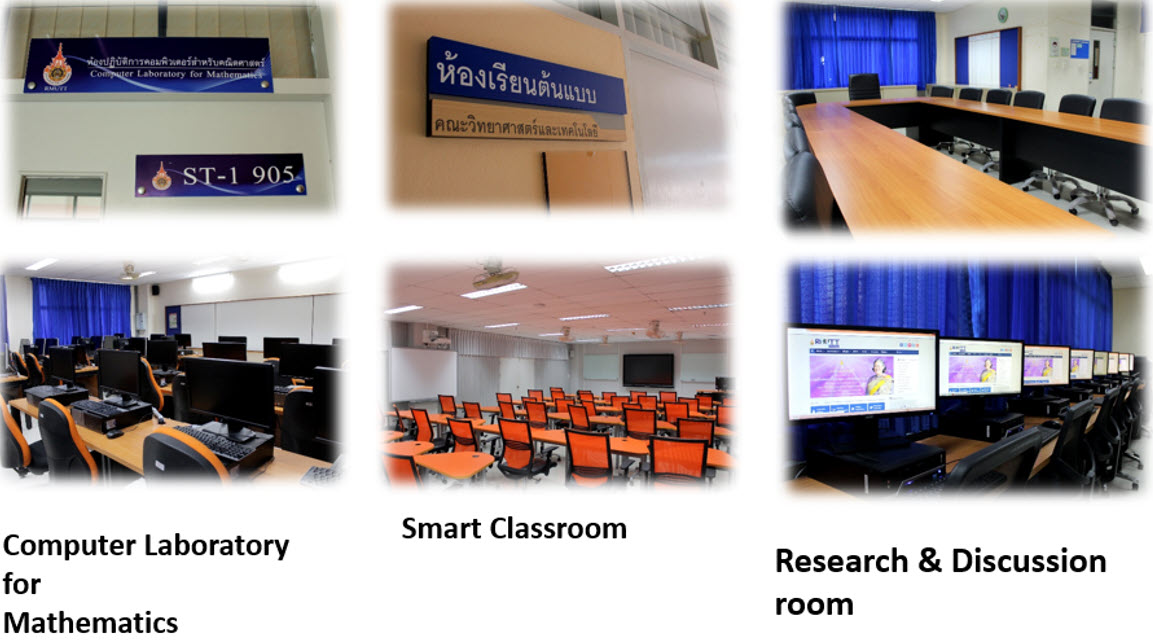
\includegraphics[width=0.8\textwidth]{Pic7.1-1.jpg}
\end{center}
%\caption{ห้องปฏิบัติการ ST-1 905, ST-1 906, ST-1 908  }
%\end{figure}
\item {\bf ห้องสมุด:}\\ {\bf ห้องสมุดของมหาวิทยาลัย} มีให้บริการหนังสือ วารสาร สื่อวิดีทัศน์ และอื่นๆ วารสารเฉพาะสำหรับหลักสูตร e-Databases e-Theses e-Newpapers ระบบสืบค้นข้อมูลทรัพยากรห้องสมุดผ่านระบบห้องสมุดอัตโนมัติ (Web OPAC) IT-Zone บริการสื่ออิเล็กทรอนิกส์ Edutainment ZONE บริการจองห้องออนไลน์ บริการวารสาร นิตยสาร หนังสือพิมพ์ บริการด้านภาษา/โปรแกรมการฝึกปฏิบัติ/ทดสอบทางภาษา (SPEEXX (CLT, Chiness Mandarin, Sanako, Euro Talk) เป็นต้น โดยห้องสมุดมหาวิทยาลัยมีพื้นที่ใช้สอย 20,000 ตารางเมตร มีหนังสือทั่วไปภาษาไทย 126,209 เล่ม หนังสือภาษาอังกฤษ 21,957 เล่ม วิทยานิพนธ์จำนวน 4,442 เล่ม งานวิจัย 4,892 เล่ม สื่ออิเล็กทรอนิกส์ 7,659 เล่ม  ฐานข้อมูล 19 ฐาน e-Book 5 ฐานข้อมูล โซนให้บริการชั้น 1 มีเครื่องคอมพิวเตอร์ให้บริการ 90 เครื่อง โซนอบรม e-library มีเครื่องคอมพิวเตอร์ให้บริการ 30 เครื่อง 
\begin{center}
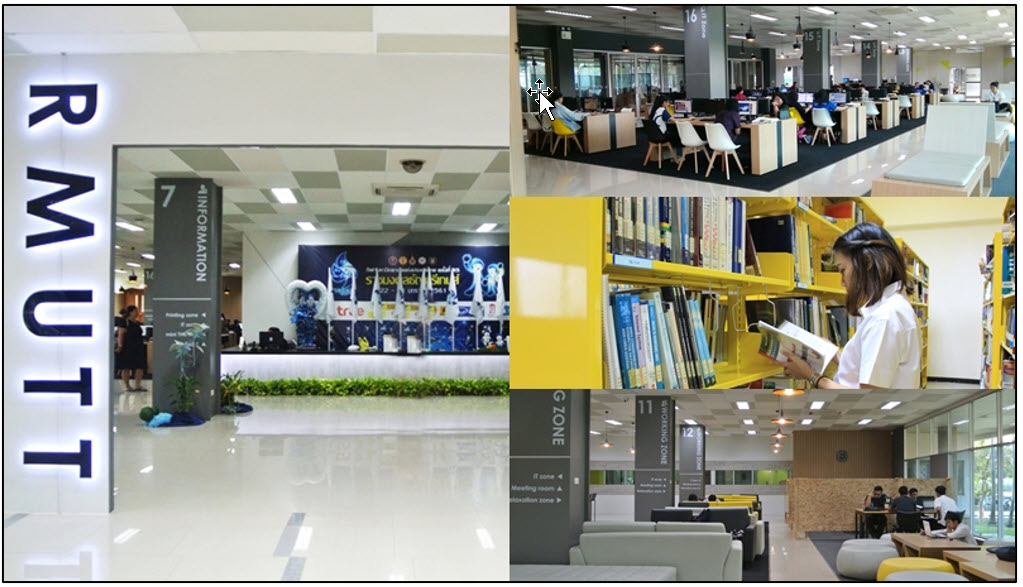
\includegraphics[width=0.8\textwidth]{Pic7.1-2.jpg}\\
\end{center}
{\bf ห้องสมุดคณะวิทยาศาสตร์และเทคโนโลยี มทร.ธัญบุรี} มีบริการยืมคืนหนังสือเฉพาะทางด้านวิทยาศาสตร์และเทคโนโลยีสำหรับนักศึกษาในสาขาวิชาต่าง ๆ (เป็นหนังสือภาษาไทย จำนวน 7,294 เล่ม หนังสือภาษาอังกฤษ จำนวน 1,184 เล่ม หนังสืออ้างอิงภาษาไทย จำนวน 11 เล่ม หนังสืออ้างอิงภาษาอังกฤษจำนวน 10 เล่ม หนังสือนวนิยาย จำนวน 39 เล่ม เรื่องสั้น จำนวน 15 เล่ม) บริการห้อง Discussion Room จำนวน 10 ที่นั่ง ณ ชั้น 4 ห้องสมุด คณะวิทยาศาสตร์และเทคโนโลยี มทร.ธัญบุรี บริการตอบคำถามและช่วยค้นคว้า
\begin{center}
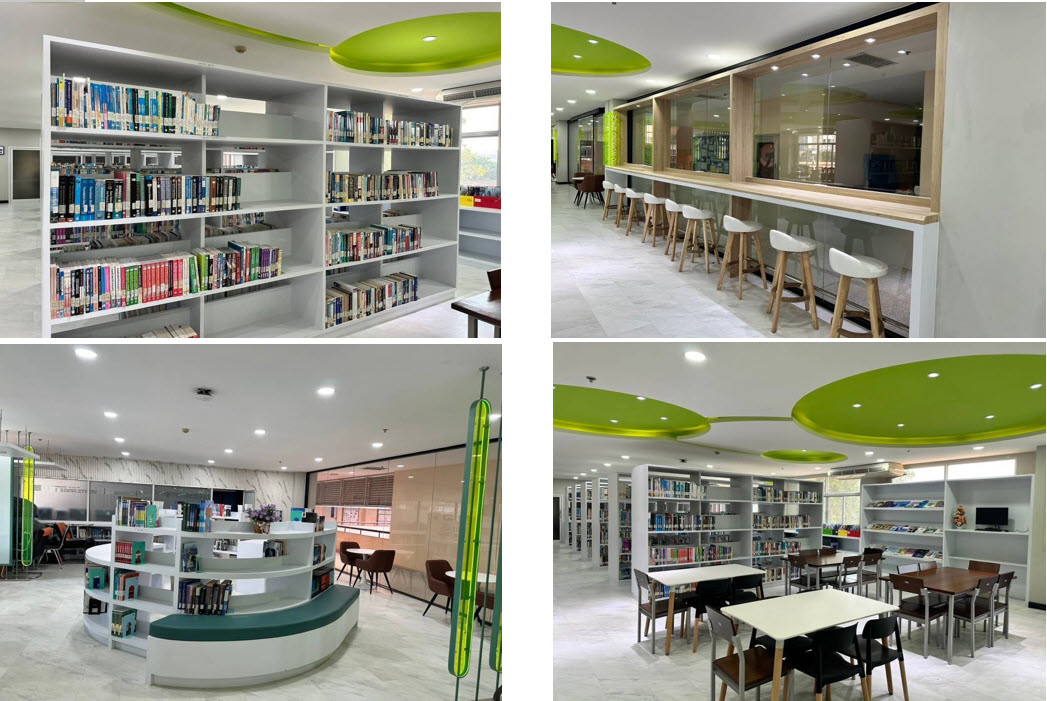
\includegraphics[width=0.8\textwidth]{Pic7.1-3.jpg}\\
\end{center}
ในส่วนของสาขาวิชามีหนังสือเฉพาะทางด้านคณิตศาสตร์  รวมทั้งเล่มโครงงานวิจัยและเล่มรายงานถอดบทเรียนรายวิชาสัมมนาของนักศึกษารุ่นพี่ สำหรับให้บริการนักศึกษา ที่ห้อง ST-1 302 และห้องST-1 908 
\begin{center}
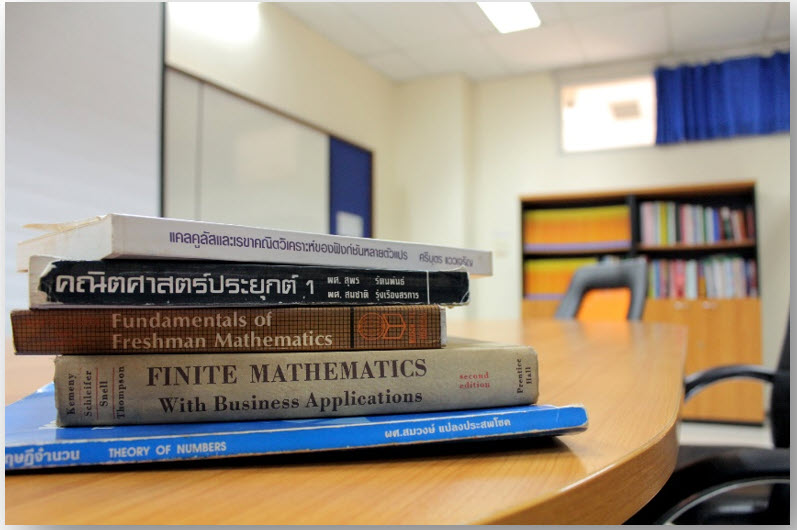
\includegraphics[width=0.8\textwidth]{Pic7.1-4.jpg}\\
\end{center}
\end{enumerate}
\begin{doclist}
	\docitem{ห้องเรียนห้องปฏิบัติการของสาขาวิชา}
	\docitem{ภาพถ่ายห้องสมุดมหาวิทยาลัย ห้องสมุดคณะ ห้องสมุดสาขาวิชา}
\end{doclist}
%%%%%%%%%%%%%%%%%%%% 7.2 %%%%%%%%%%%%%%%
\subcriteria{The laboratories and equipment are shown to be up-to-date, readily available, and effectively deployed.}

สาขาวิชาคณิตศาสตร์ประยุกต์มีห้องปฏิบัติการคอมพิวเตอร์ในความรับผิดชอบจำนวน 1 ห้อง ได้แก่ ห้องปฏิบัติการ ST-1 905 ความจุ 30 ที่นั่ง สำหรับให้บริการกับนักศึกษาที่เรียนในรายวิชาชีพ ของหลักสูตรฯ และรายวิชาชีพบางรายวิชาของหลักสูตรอื่นภายในคณะฯ ในห้องปฏิบัติการมีการลงมีโปรแกรมสำเร็จรูปที่จำเป็นสำหรับนักศึกษาสาขาวิชาคณิตศาสตร์ประยุกต์ เช่น MINITAB  SPSS โปรแกรมฟรี ที่เป็น open source เช่น โปรแกรม R  โปรแกรม Wx Maxima และ โปรแกรม Python เป็นต้น และมีการ update version ของโปรแกรมคอมพิวเตอร์อยู่เสมอเพื่อประโยชน์ในการใช้งานของอาจารย์และนักศึกษา โดยสาขาวิชามีเจ้าหน้าที่ห้องปฏิบัติการคอมพิวเตอร์ 1 คน ที่ดูแลและอำนวยความสะดวกให้กับนักศึกษาและอาจารย์ 

นอกจากนี้สาขาวิชาคณิตศาสตร์ประยุกต์ได้รับจัดสรรงบประมาณในการจัดซื้อวัสดุการศึกษาในปีการศึกษา 2566 จำนวน 43,500 บาท สำหรับนักศึกษาวิชาชีพในหลักสูตร เพื่อใช้ในการจัดซื้อวัสดุในการจัดการเรียนการสอนและปรับปรุงวัสดุต่างๆ ในห้องปฏิบัติการให้มีความพร้อมในการจัดการเรียนการสอนอยู่เสมอ



\begin{doclist}
	\docitem{ห้องปฏิบัติการของสาขาวิชา}
\end{doclist}

%%%%%%%%%%%%% 7.3 %%%%%%%%%%%%%
\subcriteria{A digital library is shown to be set-up, in keeping with progress in information and communication technology.}

หลักสูตรวิทยาศาสตรบัณฑิต สาขาวิชาคณิตศาสตร์ประยุกต์ ใช้ทรัพยากรด้านห้องสมุดดิจิทัลของ
มหาวิทยาลัย ซึ่งรับผิดชอบโดย สำนักวิทยบริการและเทคโนโลยีสารสนเทศ (สวส.) ที่ให้บริการฐานข้อมูลหนังสืออิเล็กทรอนิกส์ (e-Book) สำหรับนักศึกษา คณาจารย์ นักวิจัย และบุคลากรของมหาวิทยาลัยเทคโนโลยีราชมงคลธัญบุรี เพื่อการสืบค้นและการใช้งานฐานข้อมูลหนังสืออิเล็กทรอนิกส์สามารถเข้าถึงข้อมูลสารสนเทศตลอดจนเอกสารฉบับเต็มได้ ซึ่งบริการต่าง ๆ ประกอบไปด้วย
\begin{enumerate}
\item ฐานข้อมูลอิเล็กทรอนิกส์ ฐานข้อมูลอิเล็กทรอนิกส์เพื่อการสืบค้น เป็นการให้บริการฐานข้อมูล
อิเล็กทรอนิกส์ออนไลน์ในต่างประเทศและภายในประเทศไทย เพื่อให้บริการแก่นักศึกษา อาจารย์ บุคลากร และนักวิจัยของมหาวิทยาลัย ให้สามารถใช้ทรัพยากรและเข้าถึงข้อมูลสารสนเทศเอกสารฉบับเต็มได้สะดวก รวดเร็ว ผ่านเครือข่ายสารสนเทศของมหาวิทยาลัยฯ  ซึ่งประกอบไปด้วย 3 ส่วนคือ \\[0.2cm]

\includegraphics[width=0.9\textwidth]{Pic7.3-1.jpg}
\begin{itemize}
	\item e-Databases เป็นฐานข้อมูลอิเล็กทรอนิกส์ออนไลน์ต่างประเทศ สนับสนุนโดย สำนัก
	ปลัดกระทรวงการอุดมศึกษา วิทยาศาสตร์ วิจัยและนวัตกรรม (อว.) ซึ่งฐานข้อมูลที่ให้บริการประกอบด้วย ฐานข้อมูลอ้างอิง (Reference Database) จำนวน 9 ฐานข้อมูล ที่เกี่ยวกับฐานข้อมูลวารสารอิเล็กทรอนิกส์ในสาขาวิชาต่าง ๆ รวมถึงฐานข้อมูลออนไลน์ที่บอกรับโดย สำนักวิทยบริการและเทคโนโลยีสารนิเทศ มทร.ธัญบุรี
	\\[0.2cm]
	
\includegraphics[width=0.8\textwidth]{Pic7.3-2.jpg}\\
	\item e-Theses เป็นการให้บริการฐานข้อมูลอิเล็กทรอนิกส์ออนไลน์ภายในประเทศ สำหรับสืบค้น
	ผลงานทางวิชาการของมหาวิทยาลัยภายในประเทศไทย และผลงานทางวิชาการของมหาวิทยาลัยเทคโนโลยีราชมงคลธัญบุรี ซึ่งประกอบด้วย งานวิจัย วิทยานิพนธ์ บทความวิชาการ และเอกสารเผยแพร่อื่น ๆ
	\item e-Newspapers ฐานข้อมูลข่าวออนไลน์ เป็นบริการกฤตภาคข่าวออนไลน์ (Online News 
	Clipping) โดยการตัดข่าวที่น่าสนใจจากหน้าหนังสือพิมพ์ต่างๆ พร้อมกับระบุแหล่งที่มาของหนังสือพิมพ์ เช่น ฉบับที่ วันที่ข่าว หัวข่าว เนื้อหาข่าว รูปภาพประกอบ (ถ้ามี) เป็นต้น โดยรวบรวมและจัดเก็บไว้ให้บริการผ่านฐานมูลออนไลน์
\end{itemize}
\item บริการด้านภาษา เป็นการบริการโปรแกรมสำหรับฝึกทักษะทางด้านภาษา ทั้งทักษะภาษาอังกฤษ 
ภาษาจีน รวมถึงภาษาอาเซียน ซึ่งแต่ละโปรแกรมมุ่งเน้นให้ผู้รับบริการมีการพัฒนาทักษะการฟัง การพูด การอ่าน และคำศัพท์ เพื่อประยุกต์ใช้ในชีวิตประจำวัน การเรียนและการทำงานได้
\\

\includegraphics[width=0.9\textwidth]{Pic7.3-3.jpg}\\
%{\bf ภาพที่ 7.3-3} บริการด้านภาษา
\item มีระบบ DLearn@RMUTT เป็นระบบจัดการเรียนการสอนในระบบออนไลน์ให้มีบรรยากาศ
เหมือนการเรียนในห้องเรียน หรือเรียกว่า LMS (Learning Management System) นักศึกษา อาจารย์ หรือบุคลากรของมหาวิทยาลัยสามารถใช้งานระบบ RMUTT D-Learn เพื่อจัดการเรียนการสอนได้ โดยอาจารย์สามารถจัดการรายวิชาของตนเองได้ เช่น การกำหนดบทเรียนและสื่อการสอน การกำหนดงานที่ได้รับมอบหมาย การทำแบบทดสอบ เป็นต้น รวมถึงนักศึกษาสามารถเข้าเรียนออนไลน์ได้ตลอดเวลา ซึ่งเหมาะกับการเรียนแบบ Flipped Classroom รวมถึงทำงานร่วมกับเครื่องมือติดต่อสื่อสารสำหรับประชุมออนไลน์ ระหว่างอาจารย์และนักศึกษาได้
\item ให้บริการการตั้งค่าการเชื่อมต่อ เครือข่ายมหาวิทยาลัยฯ (VPN) เพื่อ Remote Desktop 
Connection, ERP หรือ การสืบค้นงานวิจัย  VPN-RMUTT เป็นระบบเครือข่ายในมหาวิทยาลัยฯ ที่อนุญาตให้คณาจารย์ บุคลากรและนักศึกษาของมหาวิทยาลัย ที่อยู่นอกสถานที่สามารถเชื่อมต่อเข้ามาในเครือข่ายส่วนตัวของมหาวิทยาลัยฯ เสมือนว่าอยู่ในเครือข่ายเดียวกับมหาวิทยาลัยฯ เพื่อให้ง่ายต่อการทำงานต่างๆ ไม่ว่าจะเป็นการเข้าใช้ Remote Desktop Connection , ERP , การสืบค้นงานวิจัย โดยการเข้าใช้งานต้องมี ชื่อผู้ใช้และรหัสผ่าน ซึ่งเป็นชุดเดียวกับ การ Login เข้าใช้งานเครือข่ายอินเทอร์เน็ต WiFi ของมหาวิทยาลัย


\end{enumerate}
\begin{doclist}
	\docitem{เว็บไซต์ห้องสมุดมหาวิทยาลัย\newline https://www.library.rmutt.ac.th/language/}
\end{doclist}

%%%%%%%%%%%%% 7.4 %%%%%%%%%%%%%%%%
\subcriteria{The information technology systems are shown to be set up to meet the needs of staff and students.}

หลักสูตรวิทยาศาสตรบัณฑิตสาขาวิชาคณิตศาสตร์ประยุกต์ ใช้ระบบเทคโนโลยีสารสนเทศที่ตอบสนองความต้องการของบุคลากรและนักศึกษา 2 ส่วน ด้วยกัน คือระบบเทคโนโลยีสารสนเทศของมหาวิทยาลัย และระบบเทคโนโลยีสารสนเทศที่คณะ ฯ พัฒนาขึ้นเอง
\begin{enumerate}
\item ระบบสารสนเทศของมหาวิทยาลัย\\
\underline{ระบบสารสนเทศที่สนับสนุนด้านการเรียนการสอน}
\begin{itemize} 
\item ระบบบริการการศึกษา (https://oreg.rmutt.ac.th/?page\_id=14908)\\ เป็นระบบสารสนเทศที่มีบทบาทอย่างมากสำหรับนักศึกษา อาจารย์ที่ปรึกษา เพราะเป็นระบบที่นักศึกษาสามารถเข้ามาติดตามข่าวสารต่าง ๆ ค้นหารายวิชาเรียน ลงทะเบียนเรียนออนไลน์ ตรวจสอบผลการลงทะเบียนเรียนและพิมพ์ใบแจ้งยอดชาระเงิน ตรวจสอบตารางเรียนและตารางสอบ ตลอดจนตรวจสอบผลการเรียนของตนเอง การยื่นคำร้องออนไลน์ การถอนรายวิชาออนไลน์ และในส่วนของอาจารย์ที่ปรึกษา ระบบ OREG อานวยความสะดวกในการติดตามความก้าวหน้าและผลการเรียนของนักศึกษาเพื่อที่ช่วยให้อาจารย์ที่ปรึกษาวางแผน ให้คำแนะนำ ตลอดจนช่วยแก้ไขปัญหาให้กับนักศึกษา\\[0.2cm]
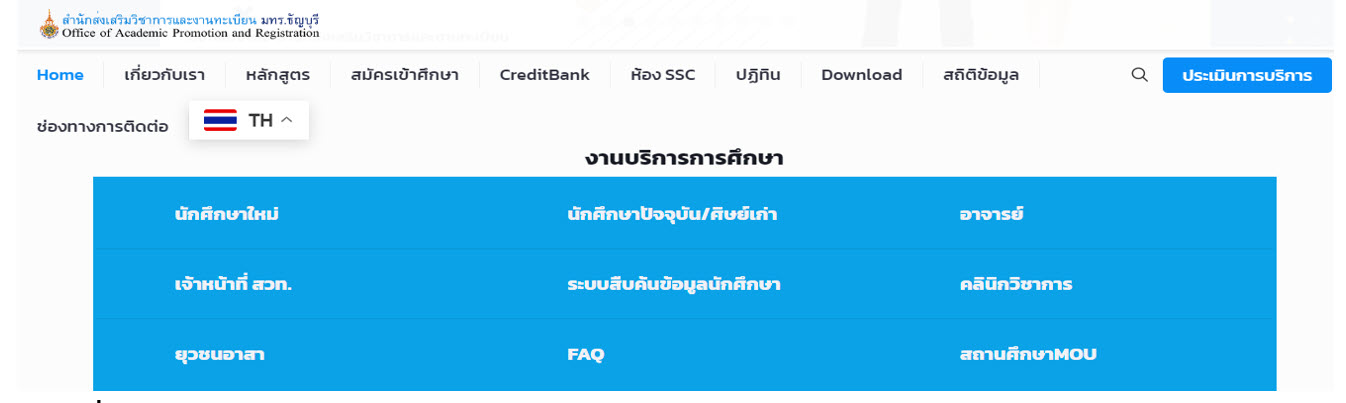
\includegraphics[width=0.8\textwidth]{Pic7.4-1.jpg}\\[0.2cm]
%\indent { \bf ภาพที่ 7.4-1} ระบบบริการการศึกษา
\item ระบบรับสมัครนักศึกษาออนไลน์ \\เป็นระบบที่อำนวยความสะดวกให้นักเรียน มัธยมศึกษาตอนปลาย หรือผู้ต้องการเข้าศึกษาต่อสามารถดำเนินการสมัครเรียนและยื่นเอกสารได้จากทุกที่ทุกเวลา ซึ่งในระบบนี้ผู้สมัครเรียนสามารถตรวจสอบผลการสอบ ดำเนินการรายงานตัว ตรวจสอบสถานะการรายงานตัว พิมพ์ใบชำระเงิน\\[0.2cm]
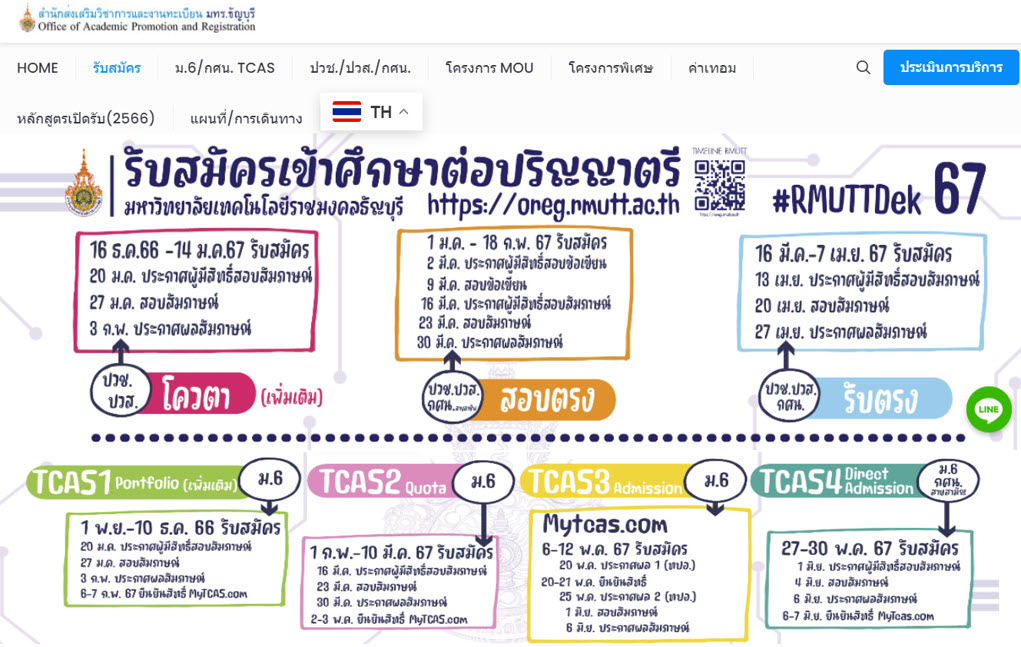
\includegraphics[width=0.8\textwidth]{Pic7.4-2.jpg}\\[0.2cm]
%\indent { \bf ภาพที่ 7.4-2} ระบบรับสมัครนักศึกษาออนไลน์
\end{itemize}
\underline{ระบบสารสนเทศสนับสนุนด้านการวิจัย}
\begin{itemize}
\item ระบบข้อมูลสารสนเทศวิจัยและนวัตกรรม มทร.ธัญบุรี ที่ช่วยในการติดตามและบริการจัดการงานวิจัยทั้งหมดจำนวน  3,440 โครงการ ทั้งงานวิจัยที่เป็นงบประมาณรายจ่าย งบประมาณรายได้ งบประมาณกองทุนส่งเสริมงานวิจัย และงบประมาณส่วนตัว ของทุกคณะ/หน่วยงาน ในมหาวิทยาลัย\\[0.2cm]
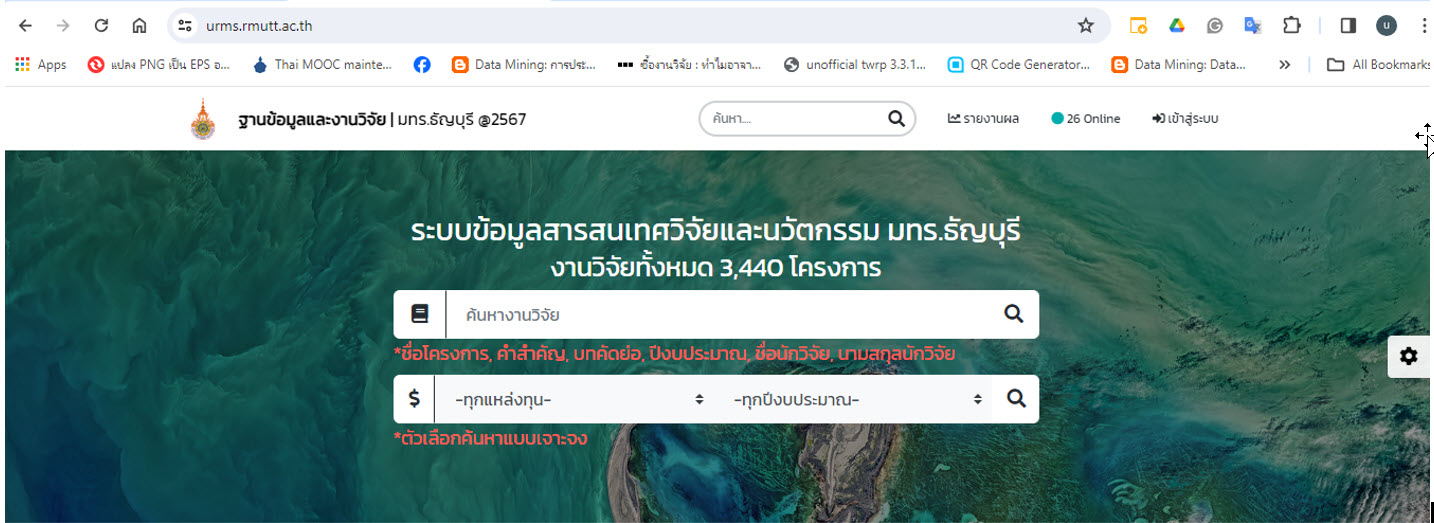
\includegraphics[width=0.7\textwidth]{Pic7.4-3.jpg}\\[0.2cm]
%\indent { \bf ภาพที่ 7.4-3} ระบบข้อมูลสารสนเทศวิจัยและนวัตกรรม มทร.ธัญบุรี
\end{itemize}
\underline{ระบบสารสนเทศที่เพื่อการบริหารจัดการ}
\begin{itemize}
	\item ระบบบุคลากรออนไลน์ (hr-online) 
	บุคลากรสามารถเข้าดูข้อมูลบุคลากรรายบุคคลประวัติการลาของบุคลากร ใบแจ้งเงินเดือน ปฏิทินการลงเวลา แจ้งผลการเลื่อนเงินเดือน เครื่องราชอิสริยาภรณ์ พิมพ์คำร้องขอแก้ไขข้อมูลประวัติส่วนตัว แสดงความคิดเห็น และสอบถามข้อมูล (ถาม-ตอบ) กราฟแสดงผลการประเมินเลื่อนเงินเดือนย้อนหลัง 5 ปี
	\item ระบบสำนักงานอิเล็กทรอนิกส์ (e-office) การบริหารจัดการเอกสารเข้า-ออก จดหมาย
	อิเล็กทรอนิกส์ การจัดเก็บเอกสาร แก้ไขเอกสาร งานเอกสารทางด้านบัญชี และการใช้ประโยชน์อื่น ๆ อีกมากมาย โดยอำนวยความสะดวกในเรื่องการลดขั้นตอน ลดระยะเวลา ลดการใช้ทรัพยากรกระดาษ (paperless) และอำนวยความสะดวกในการบริหารจัดการ การรับ-ส่งข้อมูลข่าวสาร มีการจัดเก็บเอกสารในลักษณะไฟล์ดิจิทัลอย่างเป็นระบบ มีความสะดวกรวดเร็ว และสามารถเข้าถึงและค้นหาข้อมูลได้ง่าย แม้ว่าผู้ปฏิบัติงานจะไม่อยู่ในสำนักงานก็สามารถเข้าถึงข้อมูลได้
	\item ระบบประชุมอิเล็กทรอนิกส์ (e-Meeting)
	\item ระบบจองห้องออนไลน์
\end{itemize}
\item ระบบสารสนเทศที่พัฒนาขึ้นเองโดยคณะวิทยาศาสตร์และเทคโนโลยี 
\begin{itemize}
	\item ระบบบริหารข้อมูลงานวิจัยและงานบริการวิชาการคณะวิทยาศาสตร์และเทคโนโลยี\\ เพื่อบริหารจัดการระบบบริหารข้อมูลงานวิจัยและงานบริการวิชาการ เพื่อเป็นแหล่งรวบรวมข้อมูลผลงานทางวิชาการ งานวิจัยตีพิมพ์ โครงการวิจัย งานวิจัยที่นำไปใช้ประโยชน์ นวัตกรรม ช่วยในการการค้นคว้าอ้างอิง การรายงานผล ตอบโจทย์ยุทธศาสตร์ด้านงานวิจัยและบริการวิชาการของคณะฯ และมหาวิทยาลัยฯ
	\item 	ระบบจัดการข้อมูลการประเมินบุคลากรคณะวิทยาศาสตร์และเทคโนโลยีออนไลน์\\ เพื่อช่วยบริหารจัดการเกี่ยวกับการประเมินผลการปฏิบัติราชการของบุคลากรสายวิชาการของคณะในทุกกลุ่ม ประกอบไปด้วย 
	1) พนักงานมหาวิทยาลัยวุฒิปริญญาเอก 2) พนักงานมหาวิทยาลัยวุฒิปริญญาโท 3) ข้าราชการพลเรือน 4) ข้าราชการ (ที่เป็นผู้บริหาร) และ 5) พนักงานมหาวิทยาลัยวุฒิปริญญาเอก (ที่เป็นผู้บริหาร) 
\end{itemize}
\end{enumerate}

\begin{doclist}
	\docitem{ระบบสารสนเทศของมหาวิทยาลัย}
	\docitem{ระบบสารสนเทศที่พัฒนาขึ้นเองโดยคณะวิทยาศาสตร์และเทคโนโลยี}
\end{doclist}
%%%%%%%%%%% 7.5 %%%%%%%%%%%%%%%%%%%%%%%%%%
\subcriteria{The university is shown to provide a highly accessible computer and network infrastructure that enables the campus community to fully exploit information technology for teaching, research, service, and administration.}

หลักสูตรวิทยาศาสตรบัณฑิต สาขาวิชาคณิตศาสตร์ประยุกต์ ใช้ระบบโครงสร้างพื้นฐานด้านคอมพิวเตอร์และระบบเครือข่ายเทคโนโลยีสารสนเทศที่มีการจัดเตรียมและให้บริการโดยสำนักวิทยบริการและเทคโนโลยีสารสนเทศ (สวส.) โดยระบบดังกล่าวมีความทันสมัย เพียงพอ และพร้อมใช้ ตรงกับความต้องการของทั้งในด้านการเรียนการสอน การวิจัย การบริการวิชาการ และการบริหารจัดการ ซึ่งประกอบไปด้วย
\begin{enumerate}
	\item การใช้บริการเครือข่ายไร้สาย (WIFI-RMUTT) มหาวิทยาลัยเทคโนโลยีราชมงคลธัญบุรี ทางสำนักวิทยบริการและเทคโนโลยีสารสนเทศได้ให้บริการครอบคลุมทั่วทุกจุดใน มทร.ธัญบุรี เช่น
	\begin{itemize}[label=-]
	\item  บริเวณสำนักวิทยบริการและเทคโนโลยีสารสนเทศ\newline(อาคาร ICT, Training, iWork@RT, Library )
	\item อาคารเรียนตามคณะต่าง ๆ
	\item บ้านพักสวัสดิการ ข้าราชการ มทร.ธัญบุรี
	\item หอพักสวัสดิการนักศึกษา มทร.ธัญบุรี
	\item อาคารเรียนรวมและปฏิบัติการ
\end{itemize}
\hspace*{1cm}บุคลากรสามารถเข้าใช้บริการ Wifi@RMUTT ได้โดยใช้ Username : ประกอบด้วย ชื่อ
	ภาษาอังกฤษ ตามด้วยสัญลักษณ์ (\_) และตามด้วยอักษรตัวแรกของนามสกุลภาษาอังกฤษ เช่น ชื่อ Somsak Rmutt ในการกำหนด username จะกำหนดเป็น somsak\_r (ในกรณีนามสกุลตัวแรกซ้ำจะตามด้วยนามสกุลตัวแรกและตัวที่ 2 ของนามสกุล) Password : กำหนดเป็นตัวเลข 6 หลักท้ายจากรหัสบัตรประชาชน
	(โดยบุคลากรสามารถเปลี่ยน Password ได้ด้วยตนเองในภายหลัง) \\[0.2cm]
\hspace*{1cm}นักศึกษาสามารถเข้าใช้บริการ Wifi@RMUTT ได้โดยใช้ Username :  รหัสนักศึกษา 13 หลักโดยไม่ต้องใส่ขีด (-) Password : กำหนดเป็นตัวเลข 6 หลักท้ายจากรหัสบัตรประชาชน
(โดยนักศึกษาสามารถเปลี่ยน Password ได้ด้วยตนเองในภายหลัง)\\[0.2cm]
\hspace*{1cm}ในส่วนของคณะวิทยาศาสตร์และเทคโนโลยีมี 2 อาคารเรียน คือ อาคารเฉลิมพระเกียรติ ๖ รอบพระชนมพรรษา (อาคาร 9 ชั้น) และอาคารสถาบันวิจัยเคมี (อาคาร 4 ชั้น) โดยทุกชั้นของแต่ละอาคารมีจุดเชื่อมต่อสัญญาณ Wifi ทุกชั้น ทำให้สามารถใช้งานได้อย่างไม่ติดขัด \\[0.2cm]
\hspace*{1cm}นอกจากนี้ยังมีการให้บริการการใช้งาน ระบบ Backoffice กรณีที่ไม่ได้ตั้งค่า VPN สามารถตั้งค่า VPN ได้ที่ http://www.ict.rmutt.ac.th/?p=2384  หรือนำเครื่องคอมพิวเตอร์ส่วนบุคคล (Notebook) มาให้เจ้าหน้าที่ที่ สวส. ดำเนินการตั้งค่าระบบ VPN โดยทางสำนักวิทยบริการฯ มีแนวทางจะให้ครอบคลุมทั่วทุกจุดใน มทร.ธัญบุรี ภายในอนาคตเร็ว ๆ นี้
\item 	ในส่วนของคณะมีห้องปฏิบัติคอมพิวเตอร์จำนวน  16  ห้อง รวมจำนวนเครื่องคอมพิวเตอร์ที่ให้บริการนักศึกษา จำนวน 522 เครื่อง โดยมีรายละเอียดดังตาราง 
\begin{center}
%\begin{table}[]
	\begin{tabular}{|c|c|c|c|c|}
		\hline
		\textbf{ลำดับที่} & \textbf{สาขาวิชา}                                                                                                         & \textbf{ชั้น} & \textbf{ห้อง} & \textbf{จำนวนเครื่อง} \\ \hline
		1                 & -                                                                                                                         & 4             & IT\&SCI       & 20                    \\ \hline
		2                 & สาขาวิชาฟิสิกส์                                                                                                           & 7             & ST1-710       & 37                    \\ \hline
		3                 & \multirow{10}{*}{\begin{tabular}[c]{@{}c@{}}สาขาวิชาวิทยาการคอมพิวเตอร์ และ \\ สาขาวิชาเทคโนโลยีคอมพิวเตอร์\end{tabular}} & 8             & ST1-804       & 30                    \\ \cline{1-1} \cline{3-5} 
		4                 &                                                                                                                           & 8             & ST1-805       & 31                    \\ \cline{1-1} \cline{3-5} 
		5                 &                                                                                                                           & 8             & ST1-806       & 31                    \\ \cline{1-1} \cline{3-5} 
		6                 &                                                                                                                           & 8             & ST1-807       & 37                    \\ \cline{1-1} \cline{3-5} 
		7                 &                                                                                                                           & 8             & ST1-809       & 61                    \\ \cline{1-1} \cline{3-5} 
		8                 &                                                                                                                           & 8             & ST1-810       & 30                    \\ \cline{1-1} \cline{3-5} 
		9                 &                                                                                                                           & 8             & ST1-811       & 30                    \\ \cline{1-1} \cline{3-5} 
		10                &                                                                                                                           & 8             & ST1-812       & 31                    \\ \cline{1-1} \cline{3-5} 
		11                &                                                                                                                           & 8             & ST1-813       & 30                    \\ \cline{1-1} \cline{3-5} 
		12                &                                                                                                                           & 8             & ST1-814       & 31                    \\ \hline
		13                & \multirow{4}{*}{\begin{tabular}[c]{@{}c@{}}สาขาวิชาคณิตศาสตร์ และ \\ สาขาวิชาสถิติประยุกต์\end{tabular}}                  & 9             & ST1-904       & 32                    \\ \cline{1-1} \cline{3-5} 
		14                &                                                                                                                           & 9             & ST1-905       & 30                    \\ \cline{1-1} \cline{3-5} 
		15                &                                                                                                                           & 9             & ST1-912       & 36                    \\ \cline{1-1} \cline{3-5} 
		16                &                                                                                                                           & 9             & ST1-914       & 25                    \\ \hline
	\end{tabular}
%\end{table}
\end{center}
%\includegraphics[width=0.85\textwidth]{Table 7.5-1.jpg}
\item สำนักวิทยบริการฯ มีบริการ IT zone ณ อาคารวิทยบริการ จัดพื้นที่ให้ผู้ใช้บริการสามารถใช้คอมพิวเตอร์สำหรับค้นหาข้อมูลทางวิชาการ โปรแกรมการทำงาน เรียนออนไลน์ และนันทนาการ  ผู้ใช้บริการสามารถใช้บริการได้โดยต้องมี Username และ Password WiFi-RMUTT  มีบริการเครื่องคอมพิวเตอร์ สำหรับค้นหาข้อมูลทางวิชาการ โปรแกรมการทำงาน เรียนออนไลน์ และนันทนาการ  รวมทั้งหมดจำนวน 84 เครื่อง  เครื่องคอมพิวเตอร์รองรับการสั่ง พิมพ์เอกสารออนไลน์ ได้จำนวน 64 เครื่อง
\item สำนักวิทยบริการฯ มีการพัฒนาระบบสมุดบันทึกกิจกรรม (Activity RMUTT) สำหรับนักศึกษา
\item สำนักวิทยบริการฯ ให้บริการจองห้อง ประกอบไปด้วย อาคารเรียนรวมและปฏิบัติการ (Central Building)  ห้อง Discussion Room 4-15 ที่นั่ง ห้องปฏิบัติการ Computer 40-80 ที่นั่ง  ห้อง Smart Classroom ห้อง Classroom 40 - 120 ที่นั่ง  ห้องประชุม/สัมมนา 100 ที่นั่ง
\item สำนักวิทยบริการ ฯ ให้บริการระบบห้องเรียนออนไลน์ D-Learn@RMUTT สำหรับอาจารย์ผู้สอนเพื่อจัดการเรียนการสอนในระบบออนไลน์ให้มีบรรยากาศเหมือนการเรียนในห้องเรียน โดยนักศึกษา อาจารย์ หรือบุคลากรของมหาวิทยาลัยที่สนใจสามารถใช้งานระบบ D-Learn@RMUTT เพื่อจัดการเรียนการสอน อาจารย์สามารถจัดการรายวิชาของตนเองได้ เช่น การกำหนดบทเรียนและสื่อการสอน การกำหนดงานมอบหมาย การทำแบบทดสอบ เป็นต้น รวมถึงนักศึกษาสามารถเข้าเรียนออนไลน์ได้ตลอดเวลา ซึ่งเหมาะกับการเรียนแบบ Flipped Classroom รวมถึงทำงานร่วมกับเครื่องมือติดต่อสื่อสารสำหรับประชุมออนไลน์ และการจัดการเรียนการสอนออนไลน์ ผ่านระบบ MS-Teams
\end{enumerate}

\begin{doclist}
	\docitem{ข้อมูลของโครงสร้างพื้นฐานด้านคอมพิวเตอร์และเครือข่ายพื้นฐานที่จัดหาโดยคณะและมหาวิทยาลัย}
\end{doclist}


%%%%%%%%%%% 7.6 %%%%%%%%%%%%%%%%%%%%%%%%%%
\subcriteria{The environmental, health, and safety standards and access for people with special needs are shown to be defined and implemented.}

นักศึกษาของหลักสูตรส่วนใหญ่เรียนในอาคารเรียน อาคารเฉลิมพระเกียรติ ๖ รอบพระชนมพรรษา คณะวิทยาศาสตร์และเทคโนโลยี 9 ชั้น  (ห้องเรียนและห้องปฏิบัติการอยู่บริเวณชั้น 9) เป็นส่วนใหญ่  เนื่องจากเป็นตึกสูงดังนั้นองค์ประกอบด้านความปลอดภัยที่ต้องมีคือ ข้อกำหนดด้านความปลอดภัยในอาคารสูง โดยมีกฎหมายที่เกี่ยวข้องคือ
กฎกระทรวงฉบับที่ 33 (พ.ศ.2535) ฉบับที่ 47 (พ.ศ.2540) ฉบับที่ 48 (พ.ศ.2540) และฉบับที่ 50 (พ.ศ.2540) ออกตามความในพระราชบัญญัติควบคุมอาคาร พ.ศ.2522

{\bf ด้านความปลอดภัย}

การดูแลระบบไฟฟ้าและดับเพลิง เป็นหน้าที่ของงานอาคารสถานที่คณะ มีการจัดเตรียมอุปกรณ์ดับเพลิงที่พร้อมใช้งานในทุกชั้นของอาคาร มีการตรวจสอบอุปกรณ์ถังดับเพลิงสม่ำเสมอ ปีการศึกษาละ 1 ครั้งและมีการจัดการฝึกซ้อมอพยพหนีไฟ ปีการศึกษาละ 1 ครั้ง

ในทุก ๆ ห้องเรียนห้องปฏิบัติการ จะมีระบบรักษาความปลอดภัย ได้แก่
\begin{enumerate}
	\item มีระบบ smoke detector หากพบกลุ่มควันภายในห้องจะมีการแจ้งเตือนไปที่ห้องของเจ้าหน้าที่อาคารสถานที่ของคณะ
	\item มีระบบหัวดับเพลิงติดอยู่บนฝ้าเพดานเมื่อเจอความร้อนจะแตกและปล่อยน้ำในท่อออกมาเพื่อระงับการเกิดเพลิงไหม้
	\item มีตู้ควบคุมระบบไฟฟ้าเพื่อตัดไฟเมื่อเกิดเพลิงไหม้
\end{enumerate}

นอกจากนั้นยังมีการออกกฎข้อปฏิบัติในการใช้ห้องปฏิบัติการคอมพิวเตอร์ โดยมีป้ายเตือนนักศึกษา หลังเลิกใช้เครื่องคอมพิวเตอร์ในห้องปฏิบัติการควรปิดเครื่องคอมพิวเตอร์ให้เรียบร้อยก่อนออกจากห้อง เพื่อป้องกันปัญหาด้านความร้อนของอุปกรณ์คอมพิวเตอร์

{\bf ด้านสุขภาพ}

ในแต่ละปีจะมีการตรวจสุขภาพประจำปีให้กับนักศึกษาและบุคลากรทุกคน และมหาวิทยาลัยได้ดำเนินการจัดทำประกันอุบัติเหตุให้กับนักศึกษาและบุคลากรทุกคนทุกปี ตลอดจนมีการตรวจสารเสพติดในนักศึกษาเพื่อป้องกันปัญหาสารเสพติดในสถานศึกษา มีกิจกรรมอบรมให้ความรู้เกี่ยวกับอันตรายของยาเสพติด/บุหรี่ ซึ่งดำเนินการโดยกองพัฒนานักศึกษา

ด้านสาธารณูปโภคและการรักษาความปลอดภัย
คณะฯ มีการจ้างแม่บ้านในการดูแลทำความสะอาดกำจัดขยะมูลฝอยในหน่วยงานทุกวัน และจัดกิจกรรม 5 ส ภายในหน่วยงานและมีการประกวดกิจกรรม 5 ส ในทุก ๆ ปี ในแต่ละชั้นของตึกมีน้ำดื่มที่สะอาดให้บริการกับนักศึกษา
ในส่วนการเข้าถึงของบุคคลที่มีความต้องการพิเศษ (Access for People with special needs) มีการดำเนินการเช่น จัดให้มีทางลาด ขึ้น ลง อาคาร จัดให้มีลิฟต์หรือทางลาดที่ผู้พิการหรือทุพพลภาพ และคนชรา ใช้ได้  จัดให้มีห้องน้ำสำหรับผู้พิการหรือทุพพลภาพ เป็นต้น


\begin{doclist}
	\docitem{ข้อมูลมาตรฐานด้านความปลอดภัย/สิ่งแวดล้อม }
	\docitem{ข้อมูลมาตรฐานของผู้ที่มีความต้องการพิเศษ }
\end{doclist}

%%%%%%%%%%% 7.7 %%%%%%%%%%%%%%%%%%%%%%%%%%
\subcriteria{The university is shown to provide a physical, social, and psychological environment that is conducive for education, research, and personal well-being.}
\begin{enumerate}
\item {\bf ด้านสิ่งแวดล้อมทางกายภาพ}\\ 
กองอาคารสถานที่ของมหาวิทยาลัย และงานสถานที่คณะ เป็นผู้รับผิดชอบการจัดการอาคารสถานที่ ให้มีความพร้อมใช้ เพียงพอต่อจำนวนนักศึกษา โดยมีการทบทวนการจัดสิ่งอำนวยความสะดวกของนักศึกษาทุกสิ้นปีการศึกษา สิ่งอำนวยความสะดวกด้านสิ่งแวดล้อมทางกายภาพประกอบไปด้วย
\begin{enumerate}[label=(\arabic*), leftmargin=1cm]
\item อาคารเฉลิมพระเกียรติ ๖ รอบพระชนมพรรษา คณะวิทยาศาสตร์และเทคโนโลยี 9 ชั้น  ซึ่งประกอบไป
ด้วยห้องเรียน ห้องปฏิบัติการ และพื้นที่การเรียนรู้ Learning Space สำหรับนักศึกษาในการศึกษาค้นคว้าความรู้ด้วยตนเองและทำวิจัย 
\item ห้องเอนกประสงค์ ชั้น 1 (นลินวิทย์) เพื่อใช้จัดกิจกรรม หรือเวทีการประกวดต่างๆ หรือใช้ซ้อมการแสดง 
\item พื้นที่บริเวณลานปาล์มและชั้น 1 ของคณะที่ปรับทัศนียภาพเป็นลักษณะสวนหย่อม เพื่อใช้พักผ่อนหย่อนใจ 
\item ชั้น 1 อาคารเฉลิมพระเกียรติ ๖ รอบพระชนมพรรษา คณะวิทยาศาสตร์และเทคโนโลยีมีพื้นที่ให้นักศึกษานั่งทำกิจกรรมหรือรอเรียน
\item มีสนามกีฬาบริการให้กับนักศึกษา
\item มีห้องพยาบาล 
\item ที่จอดรถบริเวณรอบคณะ
\item ร้านถ่ายเอกสาร / เครื่องถ่ายเอกสาร 
\item มีรถไฟฟ้ารับส่งภายในพื้นที่ มทร.ธัญบุรี  และสกู๊ตไฟฟ้าพลังงานสะอาด ไม่ต้องเติมน้ำมัน
 รักษาสิ่งแวดล้อม
\end{enumerate}
\item {\bf ด้านสิ่งแวดล้อมทางสังคม}\\ 
กองพัฒนานักศึกษาเป็นผู้รับผิดชอบการจัดชมรม จัดกิจกรรมพัฒนาศักยภาพของนักศึกษาในภาพรวมของมหาวิทยาลัย รวมถึงคณะดำเนินการจัดโครงการพัฒนาศักยภาพของนักศึกษาในภาพรวมของคณะ ตัวอย่างของการจัดหาสิ่งแวดล้อมทางสังคม เช่น 
\begin{enumerate}[label=(\arabic*), leftmargin=1cm]
\item กิจกรรมพิเศษนอกหลักสูตร :  มีการจัดกิจกรรมพิเศษนอกหลักสูตรต่าง ๆ ให้แก่ นักศึกษาสามารถเข้าร่วมกิจกรรม เพื่อเป็นการพัฒนาและเสริมสร้างทักษะด้านต่าง ๆ เช่น พิธีการไหว้ครู โครงการปัจฉิมนิเทศนักศึกษา โครงการรับน้องใหม่ เป็นต้น
\item กิจกรรมชมรม : มีการสนับสนุนการจัดตั้งชมรมแก่นักศึกษา เช่น ชมรม green university 
\item สโมสรนักศึกษา : มีการจัดตั้งกรรมการบริหารสโมสรนักศึกษา ซึ่งมีตัวแทนจากนักศึกษาแต่ละสาขาร่วมกันวางแผนการจัดกิจกรรมที่นักศึกษาสนใจ
\item การจัดหาแหล่งงานทั้งเต็มเวลาและนอกเวลาให้แก่นักศึกษา : กองพัฒนานักศึกษา มหาวิทยาลัย และฝ่ายพัฒนานักศึกษาของคณะมีการจัดหาแหล่งงานทั้งเต็มเวลาและนอกเวลาให้แก่นักศึกษา ผ่านการจัดกิจกรรม JOB Fair RMUTT  Facebook คณะ Facebook มหาวิทยาลัย บอร์ดประชาสัมพันธ์แหล่งงาน เป็นต้น
\end{enumerate}
\item {\bf ด้านจิตใจ }\\
กองพัฒนานักศึกษา มหาวิทยาลัยเทคโนโลยีราชมงคลธัญบุรี เปิดคลินิกกำลังใจ ให้คำปรึกษา พัฒนากำลังใจ วิเคราะห์ สร้างคุณภาพชีวิตที่ดีขึ้นให้กับนักศึกษา โดยมีผู้เชี่ยวชาญและห้องบริการให้บริการการปรึกษาเชิงจิตวิทยา มุ่งส่งเสริมสุขภาวะทางจิตที่ดีแก่นักศึกษา ให้ข้อมูลเผยแพร่องค์ความรู้ทางจิตวิทยา เพื่อส่งเสริมการดำเนินชีวิตให้มีสุขภาวะทางจิตใจที่ดี มีสติรู้เท่าทัน และสามารถจัดการอารมณ์เพื่อใช้ชีวิตอย่างมีความสุข และให้บริการปรึกษาเชิงจิตวิทยาแก่นักศึกษา ทั้งทางโทรศัพท์และการเข้าพบเพื่อให้คำปรึกษาเป็นรายบุคคล 
\item {\bf ด้านเอื้ออาทรอื่น ๆ }\\
กองพัฒนานักศึกษามหาวิทยาลัยและฝ่ายพัฒนานักศึกษาคณะ เป็นผู้รับผิดชอบงานทุนการศึกษา และการให้บริการด้านต่าง ๆ ดังนี้
\begin{enumerate}[label=(\arabic*), leftmargin=1cm]
\item ทุนการศึกษา :\\ทุนการศึกษาของมหาวิทยาลัยแบ่งจัดสรรให้แก่นักศึกษาทุกคณะ/สาขาวิชา และทุนการศึกษาจากบุคคลภายนอก/สถานประกอบการภายนอก เป็นเงินทุนสนับสนุนเพื่อส่งเสริมการศึกษาจากผู้มีจิตศรัทธา หน่วยงานการศึกษา สถานประกอบการภายนอกทั้งในประเทศ และต่างประเทศ
\item ทุนให้กู้ยืมจากรัฐบาล :  \\ได้แก่ กองทุนเงินให้กู้ยืมเพื่อการศึกษา (กยศ.) และกองทุนเงินให้กู้ยืมที่ผูกพันกับรายได้ในอนาคต (กรอ.)
\item ทุนช่วยเหลือในลักษณะทุนให้เปล่า : \\ซึ่งเกิดจากความร่วมมือระหว่างสาขาวิชากับศิษย์เก่า และบุคคลทั่วไป เพื่อสนับสนุนค่าครองชีพแก่นักศึกษาทั้งในรูปแบบของตัวเงิน รวมไปถึงการจัดหางานที่เหมาะสมเพื่อมีรายได้เพิ่มเติม
\item สวัสดิการด้านต่าง ๆ เพิ่มเติม : \\การเบิกค่าสินไหมทดแทนเมื่อนักศึกษาประสบอุบัติเหตุ การขอผ่อนผันการเข้ารับราชการทหารกองประจำการ การศึกษาต่อนักศึกษาวิชาทหาร
\end{enumerate}
\end{enumerate}

\begin{doclist}
	\docitem{ข้อมูลการจัดสภาพแวดล้อมเพื่อให้เอื้อต่อสภาพแวดล้อม สังคม และจิตใจ }
\end{doclist}

%%%%%%%%%%% 7.8 %%%%%%%%%%%%%%%%%%%%%%%%%%
\subcriteria{The competences of the support staff rendering services related to facilities are shown to be identified and evaluated to ensure that their skills remain relevant to stakeholder needs.}
เจ้าหน้าที่สายสนับสนุนที่ให้บริการทางด้านสิ่งอำนวยความสะดวกและโครงสร้างพื้นฐานของคณะวิทยาศาสตร์และเทคโนโลยี ประกอบด้วย
\begin{enumerate}
	\item เจ้าหน้าที่ห้องปฏิบัติการ
	\item เจ้าหน้าที่เทคโนโลยีสารสนเทศ
	\item เจ้าหน้าที่งานห้องสมุด
	\item เจ้าหน้าที่งานอาคารสถานที่
\end{enumerate}

การกำหนดสมรรถนะของเจ้าหน้าที่สายสนับสนุนเป็นไปตามกรอบของคณะและมหาวิทยาลัย  โดยคณะมีการจัดทำคำบรรยายลักษณะงาน  (Job Description) คุณสมบัติเฉพาะตำแหน่ง  (Job Specification) ที่ชัดเจนเกี่ยวข้องกับความสามารถในการให้บริการนักศึกษา

สำหรับเจ้าหน้าที่สายสนับสนุนด้านสิ่งอำนวยความสะดวกและโครงสร้างพื้นฐานของหลักสูตรมี 1 คน
คือเจ้าหน้าที่ประจำห้องปฏิบัติการคอมพิวเตอร์ ซึ่งหลักสูตรกำหนดสมรรถนะของเจ้าหน้าที่ประจำห้องปฏิบัติการดังนี้
\begin{enumerate}
	\item มีความเชี่ยวชาญในการติดตั้งโปรแกรมคอมพิวเตอร์
	\item มีความเชี่ยวชาญในการซ่อมคอมพิวเตอร์
	\item มีความเชี่ยวชาญในการประกอบคอมพิวเตอร์
	\item สามารถให้คำแนะนำเกี่ยวกับการใช้ห้องปฏิบัติการแก่นักศึกษาได้
\end{enumerate}

ในปีการศึกษา 2566 หลักสูตรมีการประเมินความคิดเห็นในการให้บริการด้านสิ่งอำนวยความสะดวกและโครงสร้างพื้นฐานตามสมรรถนะของผู้ให้บริการ โดยใช้ระบบการประเมินที่ทางคณะฯ เป็นผู้จัดทำขึ้น เป็นการประเมินในรูปแบบออนไลน์ผ่าน Google Form โดยมีผลการการประเมินดังตาราง
ตาราง \ref{Table 7.8-1} และ \ref{Table 7.8-2} ซึ่งมีการเกณฑ์การแปลผล ดังนี้
\begin{itemize}
\item ระดับความพึงพอใจเฉลี่ย 1.00 – 1.50 มีความคิดเห็นในระดับน้อยที่สุด
\item ระดับความพึงพอใจเฉลี่ย 1.51 – 2.50 มีความคิดเห็นในระดับน้อย
\item ระดับความพึงพอใจเฉลี่ย 2.51 – 3.50 มีความคิดเห็นในระดับปานกลาง
\item ระดับความพึงพอใจเฉลี่ย 3.51 – 4.50 มีความคิดเห็นในระดับมาก
\item ระดับความพึงพอใจเฉลี่ย 4.51 – 5.00 มีความคิดเห็นในระดับมากที่สุด  
\end{itemize}
%%%%%%%%%%%%%%%%%%% อาจารย์ %%%%%%%%%%%%%%%%
  \begin{longtable}{|>{\raggedright}p{9cm}|c|c|}
	\caption{ผลการประเมินความคิดเห็นของอาจารย์ต่อการให้บริการด้านสิ่งอำนวยความสะดวกและโครงสร้างพื้นฐานตามสมรรถนะของผู้ให้บริการ}	
	\label{Table 7.8-1}\\
	\hline
	\centering{\textbf{รายการ}} & 
	{\boldmath{$\bar{x}$}} & \textbf{SD} \\ \hline
	\endfirsthead
	\caption[]{(ต่อ) ผลการประเมินความคิดเห็นของอาจารย์ต่อการให้บริการด้านสิ่งอำนวยความสะดวกและโครงสร้างพื้นฐานตามสมรรถนะของผู้ให้บริการ}	
	\\
	\hline
	\centering{\textbf{รายการ}} & 	{\boldmath{$\bar{x}$}} & \textbf{SD} \\ \hline
	\endhead
    \hline
		\textbf{เจ้าหน้าที่ห้องปฏิบัติการ}                                                                                                                                            & \textbf{4.53}                            & \textbf{0.83}          \\ \hline
		เจ้าหน้าที่มีความรู้ ความสามารถ เกี่ยวกับเครื่องมือ และ ให้คำแนะนำในการใช้เครื่องมือได้อย่างถูกต้อง                                                                           & 4.50                            & 0.84          \\ \hline
		ความสามารถของเจ้าหน้าที่ในการเตรียมห้องปฏิบัติการ เตรียมอุปกรณ์ ตรวจสอบความเรียบร้อยของอุปกรณ์ให้พร้อมใช้                                                                     & 4.67                            & 0.82          \\ \hline
		ความสมารถของเจ้าหน้าที่ในการให้คำแนะนำ ตอบปัญหา แก้ไขปัญหาในห้องปฏิบัติการ                                                                                                    & 4.50                            & 0.84          \\ \hline
		เจ้าหน้าที่ห้องปฏิบัติการให้บริการด้วยถ้อยคำสุภาพ ยิ้มแย้ม และเป็นมิตร                                                                                                        & 4.67                            & 0.82          \\ \hline
		การติดต่อขอรับบริการของท่านในแต่ละครั้งได้รับการอำนวยความสะดวกเป็นอย่างดี ไม่มีปัญหา                                                                                          & 4.50                            & 0.84          \\ \hline
		ความสะดวกในการยืม - คืน เครื่องมือ อุปกรณ์ การเข้าใช้ห้องปฏิบัติการฯ                                                                                                          & 4.33                            & 0.82          \\ \hline
		\textbf{เจ้าหน้าที่เทคโนโลยีสารสนเทศ}                                                                                                                                         & \textbf{4.53}                            & \textbf{0.83}          \\ \hline
		ความสามารถของเจ้าหน้าที่ในการดูแลระบบเครือข่ายอินเตอร์เน็ตครอบคลุมทั่วถึง                                                                                                     & 4.50                            & 0.84          \\ \hline
		เจ้าหน้าที่สามารถดูแลระบบอินเตอร์เน็ตให้มีความเร็วเหมาะสมกับการใช้งาน                                                                                                         & 4.67                            & 0.82          \\ \hline
		มีระบบสารสนเทศแจ้งข้อมูลข่าวสารที่รวดเร็ว เช่น website, Facebook, Line@                                                                                                       & 4.50                            & 0.84          \\ \hline
		ความสามารถของเจ้าหน้าที่ในการดูแลระบบเครือข่ายอินเตอร์เน็ตให้พร้อมใช้งาน                                                                                                      & 4.50                            & 0.84          \\ \hline
		เจ้าหน้าที่สามารถตอบปัญหา แก้ไขปัญหาหากมีปัญหาเกี่ยวกับระบบเครือข่าย                                                                                                          & 4.50                            & 0.84          \\ \hline
		\textbf{เจ้าหน้าที่ห้องสมุด}                                                                                                                                                  & \textbf{4.57}                            & \textbf{0.83}          \\ \hline
		เจ้าหน้าที่มีความรู้ ความสามารถ เกี่ยวกับทักษะด้านการบริหารจัดการห้องสมุด                                                                                                     & 4.67                            & 0.82          \\ \hline
		ความสามารถของเจ้าหน้าที่ในการจัดบริการสารสนเทศ                                                                                                                                & 4.50                            & 0.84          \\ \hline
		ความสมารถของเจ้าหน้าที่ในการให้คำแนะนำ ตอบปัญหา แก้ไขปัญหา                                                                                                                    & 4.50                            & 0.84          \\ \hline
		เจ้าหน้าที่ห้องสมุดให้บริการด้วยถ้อยคำสุภาพ ยิ้มแย้ม และเป็นมิตร                                                                                                              & 4.50                            & 0.84          \\ \hline
		การติดต่อขอรับบริการของท่านในแต่ละครั้งได้รับการอำนวยความสะดวกเป็นอย่างดี ไม่มีปัญหา                                                                                          & 4.67                            & 0.82          \\ \hline
		ความสะดวกในการยืม - คืน ทรัพยากรห้องสมุด                                                                                                                                      & 4.33                            & 0.82          \\ \hline
		\textbf{เจ้าหน้าที่อาคารสถานที่}                                                                                          & \textbf{4.56} & \textbf{0.83}       \\ \hline
		ความสามารถของเจ้าหน้าที่ในการดูแลอาคารสถานที่ให้มีความสะอาดเรียบร้อย                                                                                                          & 4.67                            & 0.82          \\ \hline
		ความสามารถของเจ้าหน้าที่ในการดูแลอาคารสถานที่ให้มีความปลอดภัย เช่น ทุกชั้นของอาคารต้องจัดให้มีตู้หัวฉีดน้ำดับเพลิงที่ประกอบ ด้วยหัวต่อสายฉีดน้ำดับเพลิงพร้อมสายฉีดน้ำดับเพลิง & 4.67                            & 0.82          \\ \hline
		ความสามารถของเจ้าหน้าที่ในการดูแลและบำรุงรักษาระบบสาธารณูปโภค ให้มีสภาพพร้อมใช้งาน                                                                                            & 4.50                            & 0.84          \\ \hline
		ความสามารถของเจ้าหน้าที่ในการดูแลห้องเรียน ห้องประชุมให้พร้อมใช้งานอยู่เสมอ                                                                                                   & 4.50                            & 0.84          \\ \hline
		ความสามารถของเจ้าหน้าที่ในการดูแลอุปกรณ์โสตทัศนูปกรณ์วัสดุ ครุภัณฑ์ ให้พร้อมใช้งาน                                                                                            & 4.50                            & 0.84          \\ \hline
		ความสามารถของเจ้าหน้าที่ในการแก้ไขปัญหาเกี่ยวกับงานอาคารสถานที่หากมีปัญหาเกี่ยวกับงานอาคารสถานที่ เช่น ระบบไฟฟ้า ประปา                                                        & 4.50                            & 0.84          \\ \hline
		\multicolumn{1}{|r|}{\textbf{ค่าเฉลี่ยรวม}}       & \textbf{4.55}                            & \textbf{0.83}          \\ \hline

\end{longtable}

จากตารางพบว่าความคิดเห็นของอาจารย์ต่อการให้บริการด้านสิ่งอำนวยความสะดวกและโครงสร้างพื้นฐานตามสมรรถนะของผู้ให้บริการในภาพรวมอยู่ในระดับมากที่สุด ($\bar{x}$=4.55 SD=0.83) ความคิดเห็นในทุกประเด็นของการให้บริการอยู่ในระดับมากที่สุดทุกประเด็น 
%%%%%% นักศึกษา %%%%%%%%%%%%%%5
  \begin{longtable}{|>{\raggedright}p{9cm}|c|c|}
	\caption{ผลการประเมินความคิดเห็นของนักศึกษาต่อการให้บริการด้านสิ่งอำนวยความสะดวกและโครงสร้างพื้นฐานตามสมรรถนะของผู้ให้บริการ}	
	\label{Table 7.8-2}\\
	\hline
	\centering{\textbf{การให้บริการและช่วยเหลือผู้เรียน}} & 
		{\boldmath{$\bar{x}$}} & \textbf{SD}  \\ \hline
	\endfirsthead
	\caption[]{(ต่อ) ผลการประเมินความคิดเห็นของนักศึกษาต่อการให้บริการด้านสิ่งอำนวยความสะดวกและโครงสร้างพื้นฐานตามสมรรถนะของผู้ให้บริการ}	
	\\
	\hline
	\centering{\textbf{การให้บริการและช่วยเหลือผู้เรียน}} & 	{\boldmath{$\bar{x}$}} & \textbf{SD} \\ \hline
	\endhead
		\textbf{เจ้าหน้าที่ห้องปฏิบัติการ}                                                                                                                                            & \textbf{4.07}                            & \textbf{0.93}        \\ \hline
		เจ้าหน้าที่มีความรู้ ความสามารถ เกี่ยวกับเครื่องมือ และ ให้คำแนะนำในการใช้เครื่องมือได้อย่างถูกต้อง                                                                           & 4.13                            & 0.94        \\ \hline
		ความสามารถของเจ้าหน้าที่ในการเตรียมห้องปฏิบัติการ เตรียมอุปกรณ์ ตรวจสอบความเรียบร้อยของอุปกรณ์ให้พร้อมใช้                                                                     & 4.05                            & 0.88        \\ \hline
		ความสมารถของเจ้าหน้าที่ในการให้คำแนะนำ ตอบปัญหา แก้ไขปัญหาในห้องปฏิบัติการ                                                                                                    & 4.18                            & 0.93        \\ \hline
		เจ้าหน้าที่ห้องปฏิบัติการให้บริการด้วยถ้อยคำสุภาพ ยิ้มแย้ม และเป็นมิตร                                                                                                        & 4.13                            & 0.97        \\ \hline
		การติดต่อขอรับบริการของท่านในแต่ละครั้งได้รับการอำนวยความสะดวกเป็นอย่างดี ไม่มีปัญหา                                                                                          & 4.20                            & 0.94        \\ \hline
		ความสะดวกในการยืม - คืน เครื่องมือ อุปกรณ์ การเข้าใช้ห้องปฏิบัติการฯ                                                                                                          & 4.18                            & 0.90        \\ \hline
		\textbf{เจ้าหน้าที่เทคโนโลยีสารสนเทศ}                                                                                                                                         & \textbf{4.02}                            & \textbf{0.87}        \\ \hline
		ความสามารถของเจ้าหน้าที่ในการดูแลระบบเครือข่ายอินเตอร์เน็ตครอบคลุมทั่วถึง                                                                                                     & 4.03                            & 0.86        \\ \hline
		เจ้าหน้าที่สามารถดูแลระบบอินเตอร์เน็ตให้มีความเร็วเหมาะสมกับการใช้งาน                                                                                                         & 4.08                            & 0.89        \\ \hline
		มีระบบสารสนเทศแจ้งข้อมูลข่าวสารที่รวดเร็ว เช่น website, Facebook, Line@                                                                                                       & 4.13                            & 0.97        \\ \hline
		ความสามารถของเจ้าหน้าที่ในการดูแลระบบเครือข่ายอินเตอร์เน็ตให้พร้อมใช้งาน                                                                                                      & 4.00                            & 0.96        \\ \hline
		เจ้าหน้าที่สามารถตอบปัญหา แก้ไขปัญหาหากมีปัญหาเกี่ยวกับระบบเครือข่าย                                                                                                          & 4.10                            & 0.96        \\ \hline
		\textbf{เจ้าหน้าที่ห้องสมุด}                                                                                                                                                  & \textbf{4.14}                            & \textbf{0.92}        \\ \hline
		เจ้าหน้าที่มีความรู้ ความสามารถ เกี่ยวกับทักษะด้านการบริหารจัดการห้องสมุด                                                                                                     & 4.05                            & 0.88        \\ \hline
		ความสามารถของเจ้าหน้าที่ในการจัดบริการสารสนเทศ                                                                                                                                & 4.08                            & 0.86        \\ \hline
		ความสมารถของเจ้าหน้าที่ในการให้คำแนะนำ ตอบปัญหา แก้ไขปัญหา                                                                                                                    & 4.03                            & 0.89        \\ \hline
		เจ้าหน้าที่ห้องสมุดให้บริการด้วยถ้อยคำสุภาพ ยิ้มแย้ม และเป็นมิตร                                                                                                              & 3.90                            & 0.84        \\ \hline
		การติดต่อขอรับบริการของท่านในแต่ละครั้งได้รับการอำนวยความสะดวกเป็นอย่างดี ไม่มีปัญหา                                                                                          & 3.98                            & 0.89        \\ \hline
		ความสะดวกในการยืม - คืน ทรัพยากรห้องสมุด                                                                                                                                      & 4.08                            & 0.89        \\ \hline
		\textbf{เจ้าหน้าที่อาคารสถานที่}                                                                                                                                              & \textbf{4.06}                            & \textbf{0.91 }       \\ \hline
		ความสามารถของเจ้าหน้าที่ในการดูแลอาคารสถานที่ให้มีความสะอาดเรียบร้อย                                                                                                          & 4.05                            & 0.90        \\ \hline
		ความสามารถของเจ้าหน้าที่ในการดูแลอาคารสถานที่ให้มีความปลอดภัย เช่น ทุกชั้นของอาคารต้องจัดให้มีตู้หัวฉีดน้ำดับเพลิงที่ประกอบ ด้วยหัวต่อสายฉีดน้ำดับเพลิงพร้อมสายฉีดน้ำดับเพลิง & 4.15                            & 0.95        \\ \hline
		ความสามารถของเจ้าหน้าที่ในการดูแลและบำรุงรักษาระบบสาธารณูปโภค ให้มีสภาพพร้อมใช้งาน                                                                                            & 4.10                            & 0.90        \\ \hline
		ความสามารถของเจ้าหน้าที่ในการดูแลห้องเรียน ห้องประชุมให้พร้อมใช้งานอยู่เสมอ                                                                                                   & 4.15                            & 0.92        \\ \hline
		ความสามารถของเจ้าหน้าที่ในการดูแลอุปกรณ์โสตทัศนูปกรณ์วัสดุ ครุภัณฑ์ ให้พร้อมใช้งาน                                                                                            & 4.18                            & 0.93        \\ \hline
		ความสามารถของเจ้าหน้าที่ในการแก้ไขปัญหาเกี่ยวกับงานอาคารสถานที่หากมีปัญหาเกี่ยวกับงานอาคารสถานที่ เช่น ระบบไฟฟ้า ประปา                                                        & 4.20                            & 0.94        \\ \hline
		\multicolumn{1}{|r|}{\textbf{ค่าเฉลี่ยรวม}}                                                                                                                                   & \textbf{4.09}                            & \textbf{0.91}        \\ \hline

\end{longtable}

จากตารางพบว่าความคิดเห็นของนักศึกษาต่อการให้บริการด้านสิ่งอำนวยความสะดวกและโครงสร้างพื้นฐานตามสมรรถนะของผู้ให้บริการในภาพรวมอยู่ในระดับมาก ($\bar{x}$=4.09 SD=0.91) โดยมีความคิดเห็นน้อยที่สุดในประเด็นของการให้บริการด้วยถ้อยคำสุภาพ ยิ้มแย้ม และเป็นมิตรของเจ้าหน้าที่ห้องสมุด ($\bar{x}$=3.90 SD=0.84) ซึ่งทางหลักสูตรจะได้ส่งต่อข้อมูลไปยังคณะเพื่อหาแนวทางปรับปรุงการให้บริการต่อไป 


%%%%%%%%%%% 7.9 %%%%%%%%%%%%%%%%%%%%%%%%%%
\subcriteria{The quality of the facilities (library, laboratory, IT, and student services) are shown to be subjected to evaluation and enhancement.}

ในปีการศึกษา 2566 หลักสูตรได้ดำเนินการประเมินคุณภาพสิ่งสนับสนุนการเรียนรู้/สภาพแวดล้อมการเรียนรู้โดยให้นักศึกษาที่เรียนในหลักสูตร จำนวน 59 คน และอาจารย์ผู้สอน 17 คน เป็นผู้ตอบแบบสอบถาม พบว่า
\begin{itemize}
\item นักศึกษามีความพึงพอใจต่อสิ่งสนับสนุนการเรียนรู้/สภาพแวดล้อมการเรียนรู้อยู่ในระดับมาก ($\bar x=4.13, SD=0.59$)
และเมื่อพิจารณาผลการประเมินความพึงพอใจเป็นรายด้าน พบว่านักศึกษามีความพึงพอใจต่อสิ่งสนับสนุนด้านกายภาพอยู่ในระดับพึงพอใจมาก ($\bar x=4.22, SD=0.55$)  นักศึกษามีความพึงพอใจต่อสิ่งสนับสนุนด้านห้องปฏิบัติการอยู่ในระดับพึงพอใจมาก ($\bar x=4.24, SD=0.58$) โดยมีข้อเสนอแนะคือ เครื่องคอมพิวเตอร์ค่อนข้างประมวลผลช้า ทางสาขาวิชาได้ดำเนินการปรับปรุงโดยให้เจ้าหน้าที่ห้องปฏิบัติการอัพเกรดเครื่องคอมพิวเตอร์อยู่เสมอ
นักศึกษามีความพึงพอใจต่อสิ่งสนับสนุนด้านสิ่งอำนวยความสะดวกหรือทรัพยากรที่เอื้อต่อการเรียนอยู่ในระดับพึงพอใจมาก ($\bar x=3.94, SD=0.64$) ซึ่งมีรายละเอียดผลการประเมินแสดงดังตารางที่ \ref{Table:7.9-1}

\item อาจารย์มีความพึงพอใจต่อสิ่งสนับสนุนการเรียนรู้/สภาพแวดล้อมการเรียนรู้ อยู่ในระดับมาก ($\bar x =4.38, SD=0.54$)
และเมื่อพิจารณาผลการประเมินความพึงพอใจเป็นรายด้าน พบว่าอาจารย์มีความพึงพอใจต่อสิ่งสนับสนุนด้านกายภาพอยู่ในระดับพึงพอใจมาก ($\bar x=4.41, SD=0.49$)  อาจารย์มีความพึงพอใจต่อสิ่งสนับสนุนด้านห้องปฏิบัติการอยู่ในระดับพึงพอใจมาก ($\bar x=4.28, SD=0.54$)
อาจารย์มีความพึงพอใจต่อสิ่งสนับสนุนด้านสิ่งอำนวยความสะดวกหรือทรัพยากรที่เอื้อต่อการเรียนอยู่ในระดับพึงพอใจมาก ($\bar x=4.46, SD=0.58$) ซึ่งมีรายละเอียดผลการประเมินแสดงดังตาราง \ref{Table:7.9-2}
\end{itemize}
\begin{center}
	\begin{longtable}{|>{\raggedright}p{9cm}|c|c|}
		\caption{ความพึงพอใจของนักศึกษาต่อคุณภาพสิ่งสนับสนุนการเรียนรู้/สภาพแวดล้อมการเรียนรู้}
		\label{Table:7.9-1}
		\\
		\hline
		\multicolumn{1}{|c|}{\textbf{รายการประเมิน}}   & \boldmath$\bar{x}$ & \textbf{SD}   \\ \hline
		\endfirsthead
	   	\caption[]{(ต่อ) ความพึงพอใจของนักศึกษาต่อคุณภาพสิ่งสนับสนุนการเรียนรู้/สภาพแวดล้อมการเรียนรู้}
		\\
		\hline
		\multicolumn{1}{|c|}{\textbf{รายการประเมิน}}   & \boldmath$\bar{x}$ & \textbf{SD}   \\ \hline
		\endhead                                 	
			\textbf{ด้านภาพกายภาพ}                                                                                               &      &      \\ \hline
						1.   ห้องเรียนให้มีจำนวนเพียงพอกับผู้เรียน                                                                           & 3.95 & 0.53 \\ \hline
						2.   สภาพแวดล้อมภายในห้องรียนให้สะอาด มีแสงสว่างเพียงพอ เอื้อต่อการเรียน                                             & 4.19 & 0.54 \\ \hline
						3.   มีการดูแลรักษาวัสดุอุปกรณ์ในห้องปฏิบัติการให้พร้อมใช้งานอยู่เสมอ                                                & 4.32 & 0.57 \\ \hline
						4.   ระบบสาธารณูปโภค เช่น น้ำประปา ไฟฟ้า เพียงพอและเหมาะสม                                                           & 4.42 & 0.49 \\ \hline
						5.   อุปกรณ์ป้องกันภัยอัคคีภัยในบริเวณต่าง ๆ เช่น ถังดับเพลิง หัวฉีดดับเพลิง                                         & 4.29 & 0.52 \\ \hline
						6.   วัสดุ อุปกรณ์ในการจัดการเรียนการสอนมีเพียงพอกับผู้เรียน                                                         & 4.25 & 0.63 \\ \hline
						7.   มีการบริการจุดน้ำดื่มสำหรับนักศึกษาประจำชั้นต่าง ๆ                                                              & 4.08 & 0.59 \\ \hline
						\multicolumn{1}{|r|}{\textbf{เฉลี่ยด้านกายภาพ}}                                                                      & \textbf{4.22} & \textbf{0.55} \\ \hline
						\textbf{ด้านห้องปฏิบัติการ}                                                                                          &      &      \\ \hline
						1.   ห้องปฏิบัติการมีอุปกรณ์และสื่อเทคโนโลยีที่ใช้ในการสอนที่ทันสมัย  มีคุณภาพ    และพร้อมใช้งานอยู่เสมอ             & 3.76 & 0.59 \\ \hline
						2.   ห้องปฏิบัติการมีแสงสว่าง    อากาศถ่ายเท  หรือมีอุณหภูมิ  เหมาะสม                                                & 4.14 & 0.50 \\ \hline
						3.   มีการดูแลรักษาวัสดุอุปกรณ์ในห้องปฏิบัติการให้พร้อมใช้งานอยู่เสมอ                                                & 4.36 & 0.60 \\ \hline
						4.   มีโปรแกรมสำเร็จรูปที่เพียงพอและจำเป็นต่อการใช้งาน                                                               & 4.29 & 0.58 \\ \hline
						5.   เจ้าหน้าที่ห้องปฏิบัติการให้บริการด้วยถ้อยคำสุภาพ ยิ้มแย้ม และเป็นมิตร                                          & 4.36 & 0.68 \\ \hline
						6.เจ้าหน้าที่ห้องปฏิบัติการสามารถให้ความช่วยเหลือและแก้ไขปัญหาหาเฉพาะหน้าได้ทันท่วงที                                & 4.53 & 0.53 \\ \hline
						\multicolumn{1}{|r|}{\textbf{เฉลี่ยด้านห้องปฏิบัติการ}}                                                              & \textbf{4.24} & \textbf{0.58} \\ \hline
						\textbf{ด้านสิ่งอำนวยความสะดวกหรือทรัพยากรที่เอื้อต่อการเรียน}                                                       &      &      \\ \hline
						1.   สื่อและอุปกรณ์การเรียนการสอนในห้องเรียนมีความเพียงพอและมีประสิทธิภาพพร้อมใช้งาน                                 & 3.92 & 0.72 \\ \hline
						2.   มีห้อง  discussion  room    ที่อำนวยความสะดวกในการเรียนรู้และทำวิจัย                                            & 3.56 & 0.59 \\ \hline
						3.   ห้องเรียนและห้องปฏิบัติการมีอุปกรณ์และสื่อเทคโนโลยีที่ใช้ในการสอนที่ทันสมัย  มีคุณภาพ    และพร้อมใช้งานอยู่เสมอ & 4.44 & 0.59 \\ \hline
						4.   มีสถานที่สำหรับให้นักศึกษาและอาจารย์ได้พบปะ    แลกเปลี่ยนสนทนา  และทำงานร่วมกัน                                 & 3.78 & 0.61 \\ \hline
						5.   ห้องสมุดคณะฯ  มีหนังสือ  ตำรา    สิ่งพิมพ์  และวารสารวิชาการ   ทันสมัยหลากหลาย                                  & 4.02 & 0.68 \\ \hline
						\multicolumn{1}{|r|}{\textbf{เฉลี่ยด้านสิ่งอำนวยความสะดวกหรือทรัพยากรที่เอื้อต่อการเรียน}}                           & \textbf{3.94} & \textbf{0.64} \\ \hline
						\multicolumn{1}{|r|}{\textbf{เฉลี่ยในภาพรวม}}                                                                        & \textbf{4.13} & \textbf{0.59} \\ \hline
	\end{longtable}
\end{center}
\begin{center}
	\begin{longtable}{|>{\raggedright}p{9cm}|c|c|}
		\caption{ความพึงพอใจของอาจารย์ต่อคุณภาพสิ่งสนับสนุนการเรียนรู้/สภาพแวดล้อมการเรียนรู้}
		\label{Table:7.9-2}
		\\
		\hline
		\multicolumn{1}{|c|}{\textbf{รายการประเมิน}}   & \boldmath$\bar{x}$ & \textbf{SD}   \\ \hline
		\endfirsthead
		\caption[]{(ต่อ) ความพึงพอใจของอาจารย์ต่อคุณภาพสิ่งสนับสนุนการเรียนรู้/สภาพแวดล้อมการเรียนรู้}
		\\
		\hline
		\multicolumn{1}{|c|}{\textbf{รายการประเมิน}}   & \boldmath$\bar{x}$ & \textbf{SD}   \\ \hline
		\endhead                                 	

			\textbf{ด้านภาพกายภาพ}                                                                                               &               &               \\ \hline
			1.   ห้องเรียนให้มีจำนวนเพียงพอกับผู้เรียน                                                                           & 3.76          & 0.64          \\ \hline
			2.   สภาพแวดล้อมภายในห้องรียนให้สะอาด มีแสงสว่างเพียงพอ เอื้อต่อการเรียน                                             & 4.29          & 0.46          \\ \hline
			3.   มีการดูแลรักษาวัสดุอุปกรณ์ในห้องปฏิบัติการให้พร้อมใช้งานอยู่เสมอ                                                & 4.41          & 0.49          \\ \hline
			4.   ระบบสาธารณูปโภค เช่น น้ำประปา ไฟฟ้า เพียงพอและเหมาะสม                                                           & 4.71          & 0.46          \\ \hline
			5.   อุปกรณ์ป้องกันภัยอัคคีภัยในบริเวณต่าง ๆ เช่น ถังดับเพลิง หัวฉีดดับเพลิง                                         & 4.88          & 0.32          \\ \hline
			6.   วัสดุ อุปกรณ์ในการจัดการเรียนการสอนมีเพียงพอกับผู้เรียน                                                         & 4.53          & 0.50          \\ \hline
			7.   มีการบริการจุดน้ำดื่มสำหรับนักศึกษาประจำชั้นต่าง ๆ                                                              & 4.29          & 0.57          \\ \hline
			\multicolumn{1}{|r|}{\textbf{เฉลี่ยด้านกายภาพ}}                                                                      & \textbf{4.41} & \textbf{0.49} \\ \hline
			\textbf{ด้านห้องปฏิบัติการ}                                                                                          &               &               \\ \hline
			1.   ห้องปฏิบัติการมีอุปกรณ์และสื่อเทคโนโลยีที่ใช้ในการสอนที่ทันสมัย  มีคุณภาพ    และพร้อมใช้งานอยู่เสมอ             & 4.06          & 0.64          \\ \hline
			2.   ห้องปฏิบัติการมีแสงสว่าง    อากาศถ่ายเท  หรือมีอุณหภูมิ  เหมาะสม                                                & 4.35          & 0.48          \\ \hline
			3.   มีการดูแลรักษาวัสดุอุปกรณ์ในห้องปฏิบัติการให้พร้อมใช้งานอยู่เสมอ                                                & 4.53          & 0.50          \\ \hline
			4.   มีโปรแกรมสำเร็จรูปที่เพียงพอและจำเป็นต่อการใช้งาน                                                               & 4.29          & 0.46          \\ \hline
			5.   มีโปรแกรมคอมพิวเตอร์และห้องปฏิบัติการคอมพิวเตอร์ที่อำนวยความสะดวกต่อนักศึกษาในการทำสัมมนาและโปรเจค              & 4.18          & 0.62          \\ \hline
			6.   มีโปรแกรมคอมพิวเตอร์และห้องปฏิบัติการคอมพิวเตอร์ที่อำนวยความสะดวกต่ออาจารย์ในการทำงานวิจัยและเตรียมการสอน       & 3.82          & 0.78          \\ \hline
			7.   เจ้าหน้าที่ห้องปฏิบัติการมีการเตรียมห้องปฏิบัติการให้พร้อมใช้งานก่อนการเรียน                                    & 4.12          & 0.68          \\ \hline
			8.   เจ้าหน้าที่ห้องปฏิบัติการให้บริการด้วยถ้อยคำสุภาพ ยิ้มแย้ม และเป็นมิตร                                          & 4.41          & 0.49          \\ \hline
			9.   เจ้าหน้าที่ห้องปฏิบัติการสามารถให้ความช่วยเหลือและแก้ไขปัญหาเฉพาะหน้าได้ทันท่วงที                               & 4.47          & 0.50          \\ \hline
			\multicolumn{1}{|r|}{\textbf{เฉลี่ยด้านห้องปฏิบัติการ}}                                                              & \textbf{4.28} & \textbf{0.54} \\ \hline
			\textbf{ด้านสิ่งอำนวยความสะดวกหรือทรัพยากรที่เอื้อต่อการเรียน}                                                       &               &               \\ \hline
			1.   สื่อและอุปกรณ์การเรียนการสอนในห้องเรียนมีความเพียงพอและมีประสิทธิภาพพร้อมใช้งาน                                 & 4.71          & 0.46          \\ \hline
			2.   มีห้อง  Smart Class Room    ที่ทันสมัยและอำนวยความสะดวกในการเรียนรู้                                            & 4.76          & 0.42          \\ \hline
			3.   ห้องเรียนและห้องปฏิบัติการมีอุปกรณ์และสื่อเทคโนโลยีที่ใช้ในการสอนที่ทันสมัย  มีคุณภาพ    และพร้อมใช้งานอยู่เสมอ & 4.41          & 0.60          \\ \hline
			4.   มีสถานที่สำหรับให้นักศึกษาและอาจารย์ได้พบปะ    แลกเปลี่ยนสนทนา  และทำงานร่วมกัน                                 & 4.18          & 0.62          \\ \hline
			5. ห้องสมุดคณะฯ  มีหนังสือ  ตำรา    สิ่งพิมพ์  และวารสารวิชาการ   ทันสมัยหลากหลาย                                    & 4.24          & 0.81          \\ \hline
			6. มีโปรแกรมคอมพิวเตอร์และห้องปฏิบัติการคอมพิวเตอร์ที่อำนวยความสะดวกต่อนักศึกษาในการทำสัมมนาและโปรเจค                & 4.06          & 0.73          \\ \hline
			7. มีโปรแกรมคอมพิวเตอร์และห้องปฏิบัติการคอมพิวเตอร์ที่อำนวยความสะดวกต่ออาจารย์ในการทำงานวิจัยและเตรียมการสอน         & 4.00          & 0.77          \\ \hline
			\multicolumn{1}{|r|}{\textbf{เฉลี่ยด้านสิ่งอำนวยความสะดวกหรือทรัพยากรที่เอื้อต่อการเรียน}}                           & \textbf{4.46} & \textbf{0.58} \\ \hline
			\multicolumn{1}{|r|}{\textbf{เฉลี่ยในภาพรวม}}                                                                        & \textbf{4.38} & \textbf{0.54} \\ \hline
			
	\end{longtable}
\end{center}
%\includepdf[pages={1-4}, pagecommand={}, scale=0.93]{Table7.9-1-3.pdf}
\begin{doclist}
	\docitem{ความพึงพอใจของนักศึกษาต่อคุณภาพสิ่งสนับสนุนการเรียนรู้/ สภาพแวดล้อมการเรียนรู้ }
	\docitem{ความพึงพอใจของอาจารย์ต่อคุณภาพสิ่งสนับสนุนการเรียนรู้/ สภาพแวดล้อมการเรียนรู้}


	\end{doclist}


\newpage
\criteria{Output and Outcomes}

\subcriteria{The pass rate, drop-out rate, and average time to graduate are shown to be established, monitored, and benchmarked for improvement.}
%%%%%%%%%%%%%%%%%%%%%%%%%%%%%%%%%%%%%%%%%%
หลักสูตรได้มีการพิจารณาจำนวนผู้สำเร็จการศึกษาและการตกออกของนักศึกษาทุก ๆ ปี มีการวิเคราะห์ข้อมูลการตกออก เพื่อติดตามดูแลให้คำปรึกษาแก่นักศึกษา และบันทึกจำนวนนักศึกษาที่คงอยู่และที่ตกออกในแต่ละปีการศึกษา จัดทำข้อมูลสรุปสาเหตุการตกออกของนักศึกษา ส่งให้ประธานหลักสูตรและหัวหน้าสาขาเพื่อใช้ในการวางแนวทางแก้ไขปัญหาต่อไป 
%%%%%%%%%%%%%%%%%%%%%%%%%%%%%%%%%%%%%%%%%%
ซึ่งมีรายละเอียดจำนวน ร้อยละของผู้สำเร็จการศึกษาและผู้ที่ตกออก ของนักศึกษาที่รับเข้าในปีการศึกษา 2561-2564 ดังตาราง\\[0.2cm]
  {\footnotesize
 	\begin{tabular}{|c|c|c|c|c|c|c|c|}
 		\hline
 		{\multirow{2}{0.11\textwidth}{ปีการศึกษา}} & {\multirow{2}{0.12\textwidth}{จำนวนรับเข้า\newline  \hspace*{0.2cm}(มีตัวตน)}} & \multicolumn{4}{c|}{ผู้สำเร็จการศึกษาตามหลักสูตร} & \multirow{2}{0.1\textwidth}{\centering{ร้อยละของผู้สำเร็จการศึกษาตามหลักสูตร}} & \multirow{2}{0.11\textwidth}{\centering{ร้อยละของ\newline ผู้ที่ตกออก}} \\
 		\cline{3-6}          &      &\multicolumn{1}{p{0.05\textwidth}|}{{ 4 ปี\newline จำนวน}}  & \multicolumn{1}{p{0.058\textwidth}|}{{ 4 ปี\newline ร้อยละ}}  & \multicolumn{1}{p{0.105\textwidth}|}{{มากกว่า 4 ปี\newline จำนวน}}     &\multicolumn{1}{p{0.105\textwidth}|}{{มากกว่า 4 ปี\newline ร้อยละ}}&      & \\\hline
 		2561     & 22    &  14  & 63.64&0 &  0  & 63.64   & 36.36   \\  \hline
 		2562     & 17    &  13  & 76.47 &0&  0 & 76.47   & 23.53  \\   \hline
 		2563     & 8     &  6   &  75  & 1 & 12.50 & 87.5   &  12.5  \\   \hline
 		2564& 33     &  22   & 66.67   &   0&  0  & 66.67   &  33.33  \\  \hline
 	\multicolumn{6}{|c|}{}&	73.57   &  27.11 \\\hline
 	\end{tabular}   
 }
 

 จากตาราง พบว่า อัตราการสำเร็จการศึกษาตามหลักสูตรโดยเฉลี่ยคิดเป็นร้อยละ 73.57 และมีส่วนอัตราการตกออกเฉลี่ยคิดเป็นร้อยละ 27.11 หลักสูตร ได้วิเคราะห์ถึงสาเหตุการตกออกของนักศึกษา พบว่านักศึกษาส่วนใหญ่จะตกออกในช่วงชั้นปีที่ 1 และชั้นปีที่ 2 ทั้งนี้มีปัญหาหลักเนื่องมากจาก 
 \begin{itemize}
 	\item นักศึกษาบางส่วนไม่ได้สนในที่จะเรียนในหลักสูตร แต่เข้ามาเรียนเนื่องจากสอบไม่ติดในหลักสูตรอื่นที่ตนเองสนใจทำให้เลือกที่จะไปสอบเข้าเรียนใหม่
 	\item นักศึกษาบางส่วนปรับตัวกับการเรียนในรั้วมหาวิทยาลัยไม่ได้ รู้สึกท้อ เข้ากับเพื่อนๆ ไม่ได้ ทำให้อยากลาออก หรือผลการเรียนไม่ดี ทำให้ถูกรีไทร์
 \end{itemize}
  
  หลักสูตรจึงหาแนวทางในการแก้ปัญหาดังกล่าว รวมถึงศึกษาแนวทางการดำเนินงานของหลักสูตรอื่นที่มีผลการดำเนินงานที่ดี เพื่อแก้ปัญหาการตกออกของนักศึกษา โดยเลือกหลักสูตรวิทยาศาสตรบัณฑิต สาขาวิชาสถิติประยุกต์ เป็นคู่เทียบ ซึ่งมีรายละเอียดผลการดำเนินงานของหลักสูตรดังนี้\\[0.25cm]
   {\footnotesize
  	\begin{tabular}{|c|c|c|c|c|c|c|c|}
  		\hline
  		{\multirow{2}{0.11\textwidth}{ปีการศึกษา}} & {\multirow{2}{0.12\textwidth}{จำนวนรับเข้า\newline  \hspace*{0.2cm}(มีตัวตน)}} & \multicolumn{4}{c|}{ผู้สำเร็จการศึกษาตามหลักสูตร} & \multirow{2}{0.1\textwidth}{\centering{ร้อยละของผู้สำเร็จการศึกษาตามหลักสูตร}} & \multirow{2}{0.11\textwidth}{\centering{ร้อยละของ\newline ผู้ที่ตกออก}} \\
  		\cline{3-6}          &      &\multicolumn{1}{p{0.05\textwidth}|}{{ 4 ปี\newline จำนวน}}  & \multicolumn{1}{p{0.058\textwidth}|}{{ 4 ปี\newline ร้อยละ}}  & \multicolumn{1}{p{0.105\textwidth}|}{{มากกว่า 4 ปี\newline จำนวน}}     &\multicolumn{1}{p{0.105\textwidth}|}{{มากกว่า 4 ปี\newline ร้อยละ}}&      & \\\hline
  		2561     & 10    &  10  & 100 &0 &  0  & 100   & 0   \\  \hline
  		2562     & 17    &  13  & 76.47 &0&  0 & 76.47   & 23.53  \\   \hline
  		2563     & 32    &  25  &  78.13  & 0 & 0 & 78.13   &  21.87  \\   \hline
  		2564& 40     &  35   & 87.50   &   1&  2.5  & 87.50   &  10  \\  \hline
  		\multicolumn{6}{|c|}{}&	85.53   &  13.85 \\\hline
  	\end{tabular}   
  }
 
 จากตาราง พบว่าหลักสูตรวิทยาศาสตรบัณฑิต สาขาวิชาสถิติประยุกต์มีอัตราการสำเร็จการศึกษาตามหลักสูตรโดยเฉลี่ยคิดเป็นร้อยละ 85.53 และมีส่วนอัตราการตกออกเฉลี่ยคิดเป็นร้อยละ 13.85 ซึ่งมีอัตราการสำเร็จการศึกษาตามหลักสูตรเฉลี่ยสูงกว่า และอัตราการตกออกเฉลี่ยต่ำกว่าหลักสูตรวิทยาศาสตรบัณฑิต สาขาวิชาคณิตศาสตร์ประยุกต์ และจากการศึกษาแนวทางการดำเนินงานของหลักสูตรวิทยาศาสตรบัณฑิต สาขาวิชาสถิติประยุกต์ ซึ่งพบว่ามีระบบการให้คำปรึกษาที่ดี มีการปรับรูปแบบการเรียนการสอนที่เน้นการประยุกต์ใช้และนักศึกษาได้ฝึกปฏิบัติมากขึ้น และมีการจัดอบรมความรู้ที่เกียวข้องกับรายวิชาในหลักสูตรเพื่อเพิมพูนองค์ความรู้ที่จําเป็นสําหรับนักศึกษา 

หลักสูตร จึงนำแนวมาปรับปรุงการดำเนินงานของหลักสูตรโดยจัดทำเป็นแผนระยะสั้นและแผนระยะยาว ดังปรากฎใน criterion 6.2 ดังนี้
 \begin{itemize}
\item จัดกิจกรรม/โครงการเพื่อสร้างแรงบัลดาลใจ
 \begin{itemize}
 	\item นำนักศึกษาไปศึกษาดูงานที่สถานประกอบการ  เพื่อให้เห็นแนวทางการนำคณิตศาสตร์ไปใช้ในการทำงานจริง
  	\item เชิญศิษย์เก่าที่ประสบความสำเร็จมาบรรยายเพื่อสร้างแรงบัลดาลใจในการเรียน
 	\item จัดกิจกรรม สานสัมพันธ์ น้อง-พี่ สาขาวิชาคณิตศาสตร์
 	\item จัดกิจกรรมแสดงความยินดีกับพี่บัณฑิตสาขาวิชาคณิตศาสตร์
 	\item จัดกิจกรรมเตรียมความพร้อมเข้าสู่รั้วมหาวิทยาลัยและปฐมนิเทศนักศึกษาใหม่สาขาวิชาคณิตศาสตร์
 	 \end{itemize}
 \item จัดกิจกรรม/โครงการเพื่อส่งเสริมความรู้ทางด้านวิชาการและวิชาชีพ
 \begin{itemize}
 	\item โครงการถ่ายทอดประสบการณ์จริงสู่การฝึกประสบการณ์วิชาชีพสาขาวิชาคณิตศาสตร์
 	\item โครงการการพัฒนาศักยภาพด้านการเรียนรู้เชิงลึกสำหรับการแก้ปัญหาในศตวรรษที่ 21
 	\item โครงการพัฒนาทักษะกระบวนการคิดและการเรียนรู้ในการส่งเสริมความเป็นนวัตกรของนักศึกษาสาขาวิชาคณิตศาสตร
 \end{itemize}
 \end{itemize}

นอกจากนี้หลักสูตรยังมีระบบการให้คำปรึกษา มีการกำกับติดตามนักศึกษาในด้านต่างๆ ทั้งทางด้านการเรียน และการใช้ชีวิตเป็นต้น เพื่อลดอัตราการตกออกและส่งเสริมให้นักศึกษาสำเร็จการศึกษาตามหลักสูตรมากขึ้น
\begin{doclist}
\docitem{ข้อมูลจำนวนนักศึกษา จำนวนนักศึกษาตกออก}
\docitem{ข้อมูลจำนวนนักศึกษาที่สำเร็จการศึกษาตามแผน และระยะเวลาการสำเร็จการศึกษาเฉลี่ย}
\end{doclist}


\subcriteria{Employability as well as self-employment, entrepreneurship, and advancement to further studies, are shown to be established, monitored, and benchmarked for improvement.}

การเก็บรวบรวมข้อมูลเกี่ยวกับภาวะการมีงานทำภายใน 1 ปี และ รายได้เฉลี่ยต่อเดือนของบัณฑิตระดับปริญญาตรี  ทางมหาวิทยาลัยได้มอบหมายให้กองพัฒนานักศึกษา (กพน.) เป็นผู้เก็บรวบรวม วิเคราะห์ และส่งผลการสำรวจกลับมาให้ทางคณะและหลักสูตร 

ในปีการศึกษา 2567 \printprogram{}
ยังไม่มีนักศึกษาสำเร็จการศึกษา หลักสููตรจึงนำข้อมูลภาวะการมีงานทำของหลักสูตร วิทยาศาสตรบัณฑิต สาขาวิชาคณิตศาสตร์(หลักสูตรปรับปรุง พ.ศ.2559) มาพิจารณา โดยมีคู่เทียบคือ หลักสูตรวิทยาศาสตรบัณฑิต สาขาวิชาคณิตศาสตร์ประยุกต์ มหาวิทยาลัยธรรมศาสตร์ โดยนำข้อมูลภาวะการมีงานทำที่เผยแพร่ผ่านเว็บไซต์ของสำนักงานปลัดกระทรวงการอุดมศึกษา วิทยาศาสตร์ วิจัยและนวัตกรรม (https://employ.mhesi.go.th/) มาใช้ในการวิเคราะห์ ซึ่งมีรายละเอียดดังตารางต่อไปนี้
 \begin{longtable}{|x{0.1\textwidth}|*{7}{x{0.07\textwidth}|}} % Adjusted column widths
	\hline
	\multicolumn{1}{|x{0.2\textwidth}|}{\textbf{ปีการศึกษา}} &
	\multicolumn{4}{x{0.4\linewidth}|}{\textbf{วท.บ.(คณิตศาสตร์) มทร.ธัญบุรี}} &
	\multicolumn{3}{x{0.3\linewidth}|}{\textbf{วท.บ.(คณิตศาสตร์ประยุกต์) ม.ธรรมศาสตร์ (คู่เทียบ)}} \\
	\cline{2-8}
	\multicolumn{1}{|x{0.07\textwidth}|}{} &
	\multicolumn{1}{x{0.07\textwidth}|}{ จำนวนบัณฑิตทั้งหมด} &
	\multicolumn{1}{x{0.07\textwidth}|}{ จำนวนบัณฑิตที่ตอบฯ} &
	\multicolumn{1}{x{0.07\textwidth}|}{ ร้อยละการได้งานทำใน 1 ปี} &
	\multicolumn{1}{x{0.07\textwidth}|}{ รายได้เฉลี่ยต่อเดือน} &
	\multicolumn{1}{x{0.07\textwidth}|}{ จำนวนบัณฑิตที่ได้งานทำ} &
	\multicolumn{1}{x{0.07\textwidth}|}{ ร้อยละการได้งานทำใน 1 ปี} &
	\multicolumn{1}{x{0.07\textwidth}|}{ รายได้เฉลี่ยต่อเดือน} \\
	\hline
	\endhead % End of table header
	
	\hline
	2564  &     14   &     11  &    71.43  &   17,300  &    16  &   66.67 & 21,591  \\
	\hline
	2565 &  14   &     11  &    100.00  &   20,272  &    26  &   72.22 & 17,955\\
	\hline
	2566 &  6   &     6  &      83.33  &   17,000  &    19  &   67.85  &  24,167 \\
	\hline
	\multicolumn{3}{|l|}{\bf เฉลี่ย}&84.92&18,191&&68.91&21,238\\	\hline
\end{longtable}
จากตารางพบว่า อัตราการได้งานทำหลังสำเร็จการศึกษาของหลักสูตรวิทยาศาสตรบัณฑิต สาขาวิชาคณิตศาสตร์ (หลักสูตรปรับปรุง พ.ศ.2559) เฉลี่ย 3 ปีย้อนหลังคิดเป็นร้อยละ 84.92 แสดงให้เห็นว่าบัณฑิตที่จบการศึกษาจาหลักสูตร ยังเป็นที่ต้องการของตลาดแรงงาน  แต่เมื่อพิจารณาเงินเดือนเฉลี่ย 3 ปีย้อนหลัง เทียบกับบัณฑิตที่จบการศึกษาหลักสูตรวิทยาศาสตรบัณฑิต สาขาวิชาคณิตศาตร์ประยุกต์ มหาวิทยาลัยธรรรมศาสตร์ พบว่า บัณฑิตที่จบการศึกษาหลักสูตรวิทยาศาสตรบัณฑิต สาขาวิชาคณิตศาตร์ประยุกต์ มหาวิทยาลัยธรรรมศาสตร์มีเงินเดือนเฉลี่ยที่สูงกว่า

อาจารย์ผู้รับผิดชอบหลักสูตรจึงร่วมกันวิเคราะห์ในประเด็นดังกล่าวซึ่งพบว่า หลักสูตรวิทยาศาสตรบัณฑิต สาขาวิชาคณิตศาสตร์ (หลักสูตรปรับปรุง พ.ศ. 2559) เป็นหลักสูตรทางด้านคณิตศาสตร์บริสุทธิ์ รายวิชาทางด้านคณิตศาสตร์ประยุกต์มีน้อย ทำให้บัณฑิตที่จบการศึกษาจากหลักสูตรส่วนใหญ่ประกอบอาชีพเป็นผู้สอนในสถาบันการศึกษาภาคเอกชน ส่วนบัณฑิตที่จบจากหลักสูตรของมหาวิทยาลัยธรรมศาสตร์ เนื่องจากหลักสูตรเป็นด้านคณิตศาสตร์ประยุกต์จึงตรงตามความต้องการของภาคธุรกิจและอุตสาหกรรมมากกว่าทำให้บัณฑิตในหลักสูตรส่วนใหญ่ทำงานในบริษัทภาคเอกชนทำให้มีเงินเดือนที่สูงกว่า

อาจารย์ผู้รับผิดชอบหลักสูตรจึงปรับปรุงกระบวนการโดย
\begin{itemize}
	\item ปรับหลักสูตรให้มีความทันสมัยโดยปรับเป็น \printprogram{} ซึ่งเป็นหลักสูตรที่ใช้อยู่ในปัจจุบัน และจะมีนักศึกษาจบการศึกษารุ่นแรกในปีการศึกษา 2567
	\item ส่งเสริมการจัดกิจกรรม/โครงการพัฒนาศักยภาพนักศึกษาในด้านต่างๆ ที่ตรงตามความต้องการของภาคอุตสาหกรรม ดังรายละเอียดการดำเนินงานใน criterion 6.2
	\item ส่งสริมให้นักศึกษาออกฝึกประสบการณ์วิชาชีพในสถานประกอบการภาคธุรกิจและอุตสาหกรรมมากขึ้น
\end{itemize}
\begin{doclist}
\docitem{ข้อมูลภาวะการมีงานทำภายใน 1 ปี ของบัณฑิต }
\docitem{ข้อมูลรายได้เฉลี่ยต่อเดือนของบัณฑิต}
\end{doclist}

\subcriteria{Research and creative work output and activities carried out by the academic staff and students, are shown to be established, monitored, and benchmarked for improvement.}
หลักสูตรมีการส่งเสริมและสนับสนุนอาจารย์ในหลักสูตรในด้านต่าง ๆ รวมทั้งด้านงานวิจัย ดังรายละเอียดใน criterion 5 โดยหลักสูตรได้มีการกำหนดตัวชี้วัดความสำเร็จในประเด็นนี้ คือ จำนวนงานวิจัยตีพิมพ์ในฐานข้อมูลสากล (scopus) ที่มีคุณภาพระดับสูง (Q1) ของอาจารย์ในหลักสูตรไม่ต่ำกว่าร้อยละ 20 ของจำนวนงานวิจัยตีพิมพ์ทั้งหมด

ซึ่งผลงานตีพิมพ์ของอาจารย์ในหลักสูตรปีการศึกษา 2564-2567 โดยมีหลักสูตรวิทยาศาสตรบัณฑิต สาขาวิชาสถิติประยุกต์ เป็นคู่เทียบ มีรายละเอียดดังตาราง 
\begin{longtable}{| >{\raggedright}p{0.3\textwidth} |c|c|c|c|c|c|c|c|} 
\hline
\multicolumn{1}{|c|}{ระดับผลงาน}&\multicolumn{4}{c|}{วท.บ.(คณิตศาสตร์ประยุกต์)}&\multicolumn{4}{c|}{วท.บ.(สถิติประยุกต์)}\\\cline{2-9}
&2564&2565&2566&2567&2564&2565&2566&2567\\\hline
Q1&14&13&6&4&19&13&9&2\\
Q2&9&6&5&1&3&5&3&5\\
Q3&4&3&2&0&8&7&3&4\\
Q4&2&2&2&0&5&2&0&1\\
TCI1&3&3&1&0&1&2&2&1\\
TCI2&2&0&0&0&3&7&2&0\\
\hline
รวม&36&27&16&5&39&36&19&13\\\hline
ร้อยละของผลงานระดับ Q1 &39&48&38&80&49&36&47&15\\\hline
จำนวนผลงานตีพิมพ์ต่ออาจารย์ในหลักสูตร&2&1.5&0.94&0.28&3.25&3&1.58&1.18\\\hline
\end{longtable}
จากตารางพบว่า ร้อยละของผลงานระดับ Q1 ของอาจารย์ในหลักสูตร ระหว่างปีการศึกษา 2564-2567 สูงกว่าเกณฑ์ที่หลักสูตรกำหนดทุกปี แต่เมื่อเทียบกับหลักสูตรวิทยาศสาสตรบัณฑิต สาขาวิชาสถิติประยุกต์ พบว่าจำนวนผลงานวิจัยตีพิมพ์ต่ออาจารย์ในหลักสูตร ของหลักสูตรวิทยาศาสตรบัณฑิต สาขาวิชาสถิติประยุกต์สูงกว่าในทุกปี 
หลักสูตรจึงทบทวนกระบวนการการดำเนินงาน ตลอดจนศึกษาแนวทางการดำเนินงานของหลักสูตรวิทยาศาสตรบัณฑิต สาขาวิชาสถิติประยุกต์ มาประกอบการปรับปรุงกระบวนการ การดำเนินงานในปีการศึกษาถัดไป โดยกำหนด KPI ให้อาจารย์ทุกท่านมีงานวิจัยตีพิมพ์ ส่งเสริมการจัดตั้งระบบพี่เลี้ยงในการเขียนงานวิจัยตีพิมพ์ในฐานข้อมูลสากล (scopus) รวมทั้งการรวมกลุ่มเพื่อทำวิจัย เป็นต้น ทั้งนี้เพื่อเป็นการส่งเสริมและสนับสนุนให้อาจารย์ทุกท่านมีผลงานวิจัยตีพิมพ์และเตรียมพร้อมสำหรับการเข้าสู่ตำแหน่งทางวิชาการในระดับที่สูงขึ้น

สำหรับการส่งเสริมนักศึกษาด้านการวิจัย หลักสูตรมีการส่งเสริมให้นักศึกษาเรียนรู้กระบวนการทำวิจัย เพื่อให้เกิดทักษะ กระบวนการคิด วิเคราะห์ คำนวณ การแก้ปัญหา การทำงานเป็นทีม การแสวงหาความรู้ และสามารถบูรณาการองค์ความรู้ที่ได้เรียนมาใช้ในการทำโครงงานในรายวิชาโครงงานด้านคณิตศาสตร์ ซึ่งโครงงานของนักศึกษาในปีการศึกษา 2564-2567 มีรายละเอียดดังนี้

\begin{enumerate}
\item[]{\bf ปีการศึกษา 2564}
\begin{itemize}
\item[(1)]  On the  $(s,t)$-Pell and  $(s,t)$-Pell-Lucas Polynomials by Matrix Methods
\item[(2)]  A New Iterative Scheme for Approximation of Fixed Points in Banach Spaces
\item[(3)]  Classes of Matrices over a Commutative Ring with Identity whose Determinant are Zero 
\item[(4)]  On Some Diophantine Equations of The Form $\frac{a}{x}+\frac{b}{y}+\frac{c}{z}=d$
\item[(5)]  การประมาณค่าที่หายไปของดัชนีคุณภาพอากาศจากสถานีวัด
\item[(6)]  การพัฒนาแบบจำลองทางคณิตศาสตร์สำหรับการจัดการความเสี่ยงและการประยุกต์ใช้
\end{itemize}

\item[]\textbf{ปีการศึกษา 2565}
\begin{itemize}
\item[(1)] Bivariate Vieta-Fibonacci-like polynomials

\item[(2)] Some new $(s,t)$-Pell and $(s,t)$-Pell-Lucas polynomials identities by matrix methods

\item[(3)]  Bi-Periodick-Pell Sequence

\item[(4)]  Convergence Theorems for Modified Three-Step Iterations in Uniformly Convex Metric Spaces 

\item[(5)]  การประมาณค่าดัชนีคุณภาพอากาศ ณ จุดที่ไม่มีสถานีวัด
\end{itemize}

\item[]\textbf{ปีการศึกษา 2566}
\begin{itemize}
\item[(1)] Bivariate Vieta-Jacobsthal-like polynomials

\item[(2)] Some Properties of Determinant of Matrices over Generalized Fibonacci Numbers and Generalized Gaussian Fibonacci Numbers

\item[(3)] การวิเคราะห์เกี่ยวกับจำนวนเพลล์และจำนวนเพลล์ลูคัส
\end{itemize}


\item[]\textbf{ปีการศึกษา 2567}
\begin{itemize}
	\item[(1)] การลงทุนในหุ้นร่วมกับออปชั่น (Investing in stocks with options)
	
	\item[(2)] A Multi-Day Multi-Hub Delivery Planning
	
	\item[(3)] Fixed point methodologies for logistic regression problem with application to Alzheimer’s disease screening     
	
	\item[(4)] Generating Music Variation through Chaotic Dynamical System Exploration
	
	\item[(5)] Generalized Vieta-Fibonacci-Type Polynomials and Generalized Vieta Pell-Type Polynomials
	
	\item[(6)] เว็บไซต์ระบบการจัดการทุนการศึกษา
	
	
	\item[(7)] On the Generalized Vieta-Pell and Vieta- Pell-Lucas polynomials by matrix methods  
	
	
	\item[(8)] On the Diophantine Equation $F^n_{x-1} + F^n_{x+1} = y^2$
	
\end{itemize}
\end{enumerate}

นอกจากนี้ในปีการศึกษา 2567 หลักสูตรยังมีการส่งเสริมให้นักศึกษาร่วมนำเสนอผลงานวิจัยในงานประชุมวิชาการระดับชาติ ดังรายละเอียด criterion 6.2

\begin{doclist}
\docitem{ข้อมูลงานวิจัยตีพิมพ์ของอาจารย์ในหลักสูตร}
\docitem{ข้อมูลโครงงานของนักศึกษา}
\docitem{ข้อมูลการส่งนักศึกษาเข้าร่วมนำเสนอผลงานในงานประชุมวิชาการ}
\end{doclist}

\subcriteria{Data are provided to show directly the achievement of the programme outcomes, which are established and monitored.}
หลักสูตรมีกระบวนการประเมินความสำเร็จของหลักสูตร โดยวิเคราะห์จากผลการบรรลุ PLOs ของนักศึกษาที่สำเร็จการศึกษาตามหลักสูตร ซึ่งหลักสูตรกำหนดเป้าหมายความสำเร็จไว้ดังนี้
\begin{itemize}
	\item นักศึกษาที่สำเร็จการศึกษาตามหลักสูตรต้องบรรลุ PLOs ของหลักสูตร ครบทุกข้อ
	\item จำนวนนักศึกษาที่บรรลุ PLOs ตั้้งแต่ระดับดีขึ้นไปไม่น้อยกว่าร้อยละ 40
\end{itemize}

ในปีการศึกษา 2567 มีนักศึกษาสำเร็จการศึกษาตามหลักสูตรจำนวน 22 คน โดยนักศึกษาทั้ง 22 คน
บรรลุ PLOs ทั้งหมดของหลักสูตร ดังรายละเอียดใน criterion 1.5  และมีจำนวนนักศึกษาที่บรรลุ PLOs ในแต่ละระดับแสดงดังตาราง
\begin{center}
	\begin{tabular}{|c|c|c|}
		\hline
		\textbf{ช่วงคะแนน}&\textbf{ระดับการบรรลุ PLOs}&\textbf{จำนวนนักศึกษา (คน)}\\\hline
		3.50-4.00&ดีมาก&3\\\hline
		3.00-3.49&ดี&8\\\hline
		2.50-2.99&ปานกลาง&10\\\hline
		2.00-2.49&น้อย&1\\\hline
		1.00-1.99&น้อยที่สุด&0\\\hline
	\end{tabular}
\end{center}

จากตารางพบว่ามีนักศึกษาที่บรรลุ PLOs ตั้้งแต่ระดับดีขึ้นไปจำนวน 11 คน คิดเป็นร้อยละ 40 และมีค่าเฉลี่ยระดับการบรรลุ PLOs ของนักศึกษาในภาพรวมอยู่ในระดับดี (คะแนนเฉลี่ย 3.04 จากคะแนนเต็ม 4) ซึ่งเห็นได้ว่าหลักสูตรมีความสำเร็จตามเป้าหมายที่กำหนดไว้


\textbf{คู่เทียบ} หลักสูตรได้นำหลักสูตรวิทยาศาสตรบัณฑิต  สาขาวิชาสถิติประยุกต์มาเป็นคู่เทียบในการดำเนินงานด้านการประเมินผลการบรรลุ PLOs ของนักศึกษา ซึ่งมีผลการประเมินการบรรลุ PLOs ของนักศึกษาที่สำเร็จการศึกษาปีการศึกษา 2567 ที่ประเมินแบบทางตรง ในภาพรวมอยู่ในระดับดี (คะแนนเฉลี่ย 4.17 จากคะแนนเต็ม 5)

จากการเปรียบเทียบพบว่าระดับคะแนนเฉลี่ยของการบรรลุ PLOs ของหลักสูตรวิทยาศาสตรบัณฑิต สาขาวิชาสถิติประยุกต์สูงกว่า นอกจากนี้เมื่อวิเคราะห์ถึงระดับการบรรลุ PLOs ของหลักสูตร พบว่านักศึกษาที่สำเร็จการศึกษาในหลักสูตรร้อยละ 50 มีคะแนนประเมินต่ำกว่าระดับดี และมีนักศึกษาร้อยละ 4.56 มีผลการประเมินอยู่ในระดับน้อย 

อาจารย์ผู้รับผิดชอบหลักสูตรจึงร่วมกันพิจารณาและทบทวนกระบวนการดำเนินงานรวมถึงการศึกษาแนวทางการดำเนินงานของหลักสูตรวิทยาศาสตรบัณฑิต สาขาวิชาสถิติประยุกต์ และวางแผนปรับปรุงการดำเนินงานด้านต่างๆ ทั้งด้านการเรียนการสอน การวัดประเมินผล และการจัดโครงการ/กิจกรรมพัฒนานักศึกษา เป็นต้นดังรายละเอียดการดำเนินการใน criterion 3,4 และ criterion 6 เพื่อส่งเสริมให้นักศึกษาบรรลุ PLOs ในระดับที่สูงขึ้น

%%%%%%%%%%%%%%%%%%%%%%%%%%%%%%%%%%%%%%%%%%%%%%%%%%%%%%%%%%%%%%%%%%%%%

\begin{doclist}
\docitem{ผลการประเมินการบรรลุผลลัพธ์การเรียนรู้ที่คาดหวังของหลักสูตร (PLOs) ของ\printprogram{}}
\docitem{ผลการประเมินการบรรลุผลลัพธ์การเรียนรู้ที่คาดหวังของหลักสูตร (PLOs) ของหลักสูตรวิทยาศาสตรบัณฑิต สาขาวิชาสถิติประยุกต์}
\end{doclist}












\subcriteria{Satisfaction level of the various stakeholders are shown to be established, monitored, and benchmarked for improvement.}

หลักสูตรรวบรวมข้อมูลย้อนกลับและการผลประเมินความพึงพอใจของผู้มีส่วนได้ส่วนเสียของหลักสูตร เพื่อนำมาพิจารณาวางแผนปรับปรุงกระบวนการพัฒนาบัณฑิตสำหรับปีการศึกษาต่อไป โดยมีเป้าหมายให้ผู้มีส่วนได้ส่วนเสียมีความพึงใจต่อหลักสูตรไม่น้อยกว่าระดับพึงพอใจมาก (คะแนนเฉลี่ยไม่น้อยกว่า 4.00) ซึ่งผู้มีส่วนได้ส่วนเสียของหลักสูตร ประกอบด้วย
\begin{enumerate}
	\item นักศึกษาทุกชั้นปี
	\item นักศึกษาชั้นปีสุดท้าย
	\item ผู้ใช้บัณฑิต
	\item อาจารย์ผู้รับผิดชอบหลักสูตร
\end{enumerate}
หลักสูตรเก็บรวบรวมข้อมูลผลการประเมินความพึงพอใจในแต่ละด้านดังนี้
\begin{enumerate}
	\item ประเมินความพึงพอใจของนักศึกษาทุกชั้นปีที่มีต่อหลักสูตร
	\item ประเมินความพึงพอใจของนักศึกษาชั้นปีสุดท้ายที่มีต่อคุณภาพหลักสูตร
	\item ประเมินความพึงพอใจของผู้ใช้บัณฑิตที่มีต่อบัณฑิตใหม่
	\item ประเมินความพึงพออาจารย์ของผู้รับผิดชอบหลักสูตรต่อการบริหารจัดการหลักสูตร
\end{enumerate}
โดยมีผลการประเมินดังตาราง \ref{Table:8.5-1}
\begin{longtable}{|>{\centering\arraybackslash}p{0.3\linewidth}|*{8}{c|}} 
\caption{ผลการประเมินความพึงพอใจหลักสูตรและคุณภาพบัณฑิตของผู้มีส่วนได้ส่วนเสีย ปีการศึกษา 2564-2567}	
	\label{Table:8.5-1}\\
	\hline
\multicolumn{1}{|>{\centering\arraybackslash}p{0.3\linewidth}|}{\textbf{การประเมินความพึงพอใจของผู้มีส่วนได้ส่วนเสีย}} &
	\multicolumn{4}{c|}{\textbf{วท.บ.(คณิตศาสตร์ประยุกต์)}} &
	\multicolumn{4}{c|}{\textbf{วท.บ.(สถิติประยุกต์)(คู่เทียบ)}} \\
	\cline{2-9}
	\multicolumn{1}{|c|}{} &
	\multicolumn{1}{c|}{2564} &
	\multicolumn{1}{c|}{2565} &
	\multicolumn{1}{c|}{2566} &
	\multicolumn{1}{c|}{2567} &
	\multicolumn{1}{c|}{2564} &
	\multicolumn{1}{c|}{2565} &
	\multicolumn{1}{c|}{2566} &
	\multicolumn{1}{c|}{2567} \\
	\hline
	\endhead
	
	นักศึกษาทุกชั้นปี & 4.28 & 4.29 & 4.62 & 4.69 & 4.75 & 4.77 & 4.70 & 4.73 \\
	\hline
	นักศึกษาชั้นปีสุดท้าย & 4.60 & 4.43 & 4.38 & 4.79 & 4.48 & 4.24 & 4.26 & 4.09 \\
	\hline
	ผู้ใช้บัณฑิต & 4.46 & 4.58 & 4.67 & - & 4.24 & 4.62 & 4.87 & - \\
	\hline
	อาจารย์ผู้รับผิดชอบหลักสูตร & 4.62 & 4.68 & 4.51 & 4.73 & 4.98 & 4.99 & 4.94 & 4.95 \\
	\hline

\end{longtable}




จากตาราง \ref{Table:8.5-1} ผลการประเมินความพึงพอใจของผู้มีส่วนได้ส่วนเสียเปรียบเทียบ 4 ปีย้อนหลัง พบว่าระดับความพึงพอใจอยู่ในระดับพึงพอใจมากถึงมากที่สุดในทุกด้าน และมีแนวโน้มสูงขึ้นในเกือบทุกกลุ่มของผู้มีส่วนได้ส่วนเสีย ซึ่งเป็นไปตามเป้าหมายที่หลักสูตรกำหนด แสดงให้เห็นว่าการบริหารและการดำเนินงานของหลักสูตรมีประสิทธิภาพ และบัณฑิตมีคุณภาพ

อย่างไรก็ตามเมื่อพิจารณาเทียบกับผลการดำเนินงานของหลักสูตรวิทยาศาสตรบัณฑิต สาขาวิชาสถิติประยุกต์พบว่า ระดับความพึงพอใจของผู้มีส่วนได้ส่วนเสียของหลักสูตรวิทยาศาสตรบัณฑิต สาขาวิชาสถิติประยุกต์ สูงกว่าในเกือบทุกกลุ่มของผู้มีส่วนได้ส่วนเสีย 

%หลักสูตรจึงได้ร่วมกันทบทวนและพิจารณาในรายประเด็นเพื่อปรับปรุงกระบวนการต่าง ๆ ให้ดียิ่งขึ้น ซึ่ง
%จากผลการวิเคราะห์แบบสอบถาพบว่านักศึกษามีข้อเสนอแนะ ดังนี้
%\begin{enumerate}
%	\item อยากให้หลักสูตรเสริมรายวิชาที่เกี่ยวข้องกับวิชาที่เกี่ยวข้องกับ AI หรือ ML
%    \item อยากให้หลักสูตรเน้นการปฎิบัติจริงให้มากขึ้น เช่น การเขียนโปรแกรมคอมพิวเตอร์
%\end{enumerate}
%และอาจารย์ผู้รับผิดชอบหลักสูตรมีข้อเสนอแนะ ดังนี้
%\begin{enumerate}
%	\item ควรพัฒนากระบวนการเตรียมความพร้อมอาจารย์ใหม่เพื่อรองรับการพิจารณาเสนอชื่อเป็นอาจารย์ประจำหลักสูตร 
%    \item ควรกำกับติดตามการเสนอขอตำแหน่งทางวิชาการของอาจารย์ประจำหลักสูตรเป็นรายบุคคลอย่าง
%     ใกล้ชิดยิ่งขึ้น
%      \item ควรเร่งการก้าวเข้าสู่การเสนอขอตำแหน่งทางวิชาการของอาจารย์ประจำหลักสูตรอย่างเร่งด่วน
%\end{enumerate}

จากการวิเคราะห์ผลการประเมินเป็นรายประเด็นและข้อเสนอแนะ รวมทั้งจากการศึกษาแนวทางการดำเนินงานของหลักสูตรวิทยาศาตรบันฑิต สาขาวิชาสถิติประยุกต์ อาจารย์ผู้รับผิดชอบหลักสูตรได้ร่วมกันทบทวนในแต่ละประเด็นเพื่อวางแผนปรับปรุงกระบวนการต่างๆ ให้ดีขึ้น ประกอบด้วยปรับปรุงกระบวนการจัดการเรียนการสอน การประเมินผล  การจัดโครงการส่งเสริมนักศึกษา และรวมรวมข้อมูลสำหรับใช้ในการปรับปรุงหลักสูตรต่อไป 



\begin{doclist}
\docitem{ผลการประเมินความพึงพอใจของนักศึกษาทุกชั้นปีที่มีต่อหลักสูตร}
\docitem{ผลการประเมินความพึงพอใจของนักศึกษาชั้นปีสุดท้ายที่มีต่อคุณภาพหลักสูตร}
\docitem{ผลการประเมินความพึงพอใจของผู้ใช้บัณฑิตที่มีต่อบัณฑิตใหม่}
\docitem{ผลการประเมินความพึงพอใจของอาจารย์ผู้รับผิดชอบหลักสูตรต่อการบริหารจัดการหลักสูตร}
\end{doclist}



























